\documentclass{cmspaper}
\usepackage{graphicx}
\usepackage{amsmath}
\usepackage{amssymb}
\usepackage{subfigure}
\usepackage{multirow}
\usepackage[pdfborder=0 0 0,
            colorlinks,
            urlcolor = blue,
            linkcolor = black,
            citecolor = black,
            menucolor = black,]
           {hyperref}
%% \usepackage[colorlinks]{hyperref}
%% \usepackage{url}
\usepackage[toc,page]{appendix}
\renewcommand{\appendixname}{Appendix}
%% \renewcommand{\appendixtocname}{List of appendices}

% % useful definitions

% processes
\def\dyee {\ensuremath{Z/\gamma^*\to ee}}
\def\dymm {\ensuremath{Z/\gamma^*\to\mu\mu}}
\def\dytt {\ensuremath{Z/\gamma^*\to\tau\tau}}
\def\zee {\ensuremath{Z\to ee}}
\def\zmm {\ensuremath{Z\to\mu\mu}}
\def\ztt {\ensuremath{Z\to\tau\tau}}
\def\ttbar {\ensuremath{t\bar{t}}}
\def\wwll {\ensuremath{WW\to l^+l^-}}
\def\wwlulu{\ensuremath{WW\to l^+\nu l^-\bar{\nu}}}
\def\ww {\ensuremath{WW}}
\def\wz{\ensuremath{WZ}}
\def\zz{\ensuremath{ZZ}}
\def\wgamma{\ensuremath{W\gamma}}
\def\wjets{\ensuremath{W+}jets} 
\def\tw{\ensuremath{tW}} 
\def\singletopt{\ensuremath{t} ($t$-chan)} 
\def\singletops{\ensuremath{t} ($s$-chan)} 
\def\all{all}
\def\ee{\ensuremath{ee}}
\def\emu{\ensuremath{e\mu}}
\def\mm{\ensuremath{\mu\mu}}

%units

%others
\def\pt{\ensuremath{p_T}}
\def\ipb{pb\ensuremath{^{-1}}}
\def\ifb{fb\ensuremath{^{-1}}}
\def\et{\ensuremath{E_T}}
\def\met{\ensuremath{E\!\!\!\!/_T}}
\def\fBrem{\ensuremath{f_{\rm brem}}}
\def\pin{\ensuremath{p_{\rm in}}}
\def\pout{\ensuremath{p_{\rm out}}}

\input{commands}

\setcounter{topnumber}{1}
\setcounter{bottomnumber}{1}

%===================================================================================================
\begin{document}
\begin{titlepage}

  \analysisnote{2011/XXX}

  \date{\today}

  \title{A Higgs Boson Search in the Fully Leptonic $W^+W^-$ Final State}

  \input{authors}

  \begin{abstract}
    This note describes a search for the Higgs boson in the $\WW \to 2\ell2\nu$ final state with
    a focus on \intlumi of $pp$ collision data at $\sqrt s = 7~\TeV$. We search for Higgs candidate events in
    $ee$, $\mu\mu$ and $e\mu$ channels with 0, 1 and 2 reconstructed jets in the final state. 
  \end{abstract} 

\end{titlepage}
\tableofcontents
%\listoftables
%\listoffigures
%\newpage 

%===================================================================================================
\section{Introduction}
  \label{sec:overview}
  Drell-Yan (\dyll) events represent the major background to a \hww~ signal in the same flavor final state.
After applying tight cuts on \met, they are highly suppressed but the expected signal yield is significantly 
reduced and the remaining \dyll~ background is difficult to estimate.
The net effect is that the sensitivity of the \hww~ analysis is dominated by the opposite flavor final state.

In the published 2011 analysis\cite{ref:hwwpaper}, the \dyll~ background is estimated using a method called \routin\cite{ref:hwwsmurfs}, 
which extrapolates to the signal region the \dyll~ yield in the $Z$ peak region. 
Results from the \routin method are generally stable but suffer from large statistical and systematic uncertainties.

In addition, the analysis relied on MC for deriving the shapes used in the BDT analysis; 
given that the Drell-Yan Monte Carlo sample with generator cut \mll$<$20 \GeVcc contained too few events and the statistical uncertainty 
in that region was too large, in the same flavor final state a \mll$>$ 20\GeVcc cut was applied and a significant fraction 
of a low-mass Higgs signal was lost.

The present note describes a new method for \dyll~estimation constituting a valid alternative 
to \routin, that can cross-check its results, provide shapes from data and possibly reduce the uncertainties.
The main idea is to use a ``fake-rate'' mathod, where the rate for \dyll\ events passing the final \met\ selection
is evaluated on a \gjets\ sample and applied to same flavor dilepton events in a loose \met\ region. 

  
\section{Event Selection}
  \label{sec:selection} 
  The fully leptonic final state consists of two isolated leptons
and large missing energy from the two undetectable neutrinos.
The major reducible background processes are \ttbar{}, \wjets{} and Drell-Yan. 
We thus perform several steps to select and extract the $\WW$ signal from data:

\begin{enumerate}
    \item We select events that pass pre-defined lepton triggers.
    \item We then select those events with two oppositely charged 
    high $\pt$ isolated leptons ($ee$, $\mu\mu$, $e\mu$) requiring:
        \begin{itemize}    
            \item $\pt>20~\GeVc$ for both leptons;
            \item standard identification and isolation requirements 
	    on both leptons.
        \end{itemize}
     \item We reject events with more than zero reconstructed jets;
     \item large transverse missing energy due to the neutrinos.
\end{enumerate}

The selection steps are now described in detail below.


   \subsection{Trigger}
     \label{sec:sel_trigger}
     Triggering on Higgs boson decays in the dilepton final state increases 
in difficulty with increasing instantaenous luminosity.
Single lepton triggers can only be sustained with very tight identification and
isolation requirements and large transverse momentum thresholds.
This means that double lepton triggers are the only viable option to maintain
sensitivity to a low mass Higgs boson, where the leptons transverse momentum
can be small.

We designed a suite of signal and control triggers appropriate for this analysis.
These dilepton triggers have a high efficiency to collect Higgs boson events
and are sufficiently loose to collect control events to estimate
fake lepton backgrounds and selection efficiencies with adequate precision. The detailed 
trigger paths were described in~\cite{HWW2011}.

   \subsection{Primary Vertex Reconstruction}
     \label{sec:sel_pv}
     Primary vertices are reconstructed using the so-called Deterministic Annealing (DA) 
clustering of tracks.  Reconstructed primary vertices are required to have a
$z$ position within 24~cm of the nominal detector center and a radial position within 
2~cm of the beamspot.  There must also be greater than four degrees of freedom in
the fitted vertex.  From the set of primary vertices in the event passing these
selection cuts, the vertex with the largest summed squared-$\pt$ of the associated
tracks is chosen as the event primary vertex.  Reconstructed leptons will be required 
to have small impact parameters with respect to this vertex.

Due to the fast evolution of the LHC machine, with a rapid rise in the instantaneous
luminosity, the data taking conditions have changed rapidly. 
In particular it is difficult to exactly reproduce the number of overlapping 
events (i.e. pileup) between data and simulation, and thus there will be differences
in the number of reconstructed primary vertices.
We can correct this disagreement by reweighting the simulation to
match the distribution in data. Details about the reweighting procedure are
reported in Appendix~\ref{app:vertex_reweight}.


   \subsection{Muon Selection} 
     \label{sec:sel_muons}
    Muons in CMS are reconstructed as either $StandAloneMuons$ (track
in the muon detector with low momentum resolution), $GlobalMuons$
(outside-in approach seeded by a $StandAloneMuon$ with a global fit
using hits in the muon, silicon strip and pixel 
detectors) and $TrackerMuons$ (inside-out approach seeded by an offline 
silicon strip track, using the muon detector only for muon identification 
without refitting the track). Most good quality muons are reconstructed as 
all three types at the same time and the momentum resolution is dominated by the inner
tracker system up to about 200~$\GeVc$ in transverse momentum. Details about the
optimization at low $\pt$ are given in Appendix~\ref{app:mus}. The specific
requirements to select good prompt isolated muons are the following:
\begin{itemize}
\item the muon must be found by both the global and tracker muon algorithms;
\item the global muon must have at least one good muon hit;
\item the tracker muon must have at least two matches to muon segments in 
      different muon stations;
\item more than 10 hits in the inner tracker;
\item at least one pixel hit;
\item $\chi^2/{\mathrm{ndof}} < 10$ on a global fit;
\item impact parameter in the transverse plane $|d_{0}| < 0.02~(0.01)$~cm for
      muons with $\pt$ greater (smaller) than 20 $\GeVc$,
      calculated with respect to the primary vertex;
\item longitudinal impact parameter $|d_{z}| <0.2$~cm,
      calculated with respect to the primary vertex;
\item pseudorapidity $|\eta|$ must be smaller than 2.4;
\item relative \pt\ resolution is better than 10\%.
\end{itemize}

Furthermore, the particle flow candidate-based isolation variable is 
used to reduce the contamination from the non-isolated muons originating from
jets. 

\begin{itemize}
\item $\rm{Iso}_{PF}$: defined as the scalar sum of the \pt\ of the 
    particle flow candidates satisfying the following requirements:
    \begin{itemize}
    \item $\Delta R~<~0.3$ to the muon in the $\eta \times \phi$ plane,
    \item $|d_{z}(\mathrm{PF Candidate}) - d_{z}(\mathrm{muon})| < 0.1$~cm, if the PF candidate is charged,
    \item \pt $>1.0$ GeV, if the PF candidate is classified as a neutral hadron or a photon.
    \end{itemize}
\end{itemize}

We require $\frac{\rm{Iso}_{PF}}{\pt}~<~0.13~(0.06)$ for muons in the barrel 
with $\pt$ greater (smaller) than 20 $\GeVc$. For muons in the endcap, we
require $\frac{\rm{Iso}_{PF}}{\pt}~<~0.09~(0.05)$ for muons with $\pt$ 
greater (smaller) than 20 $\GeVc$. Further details of the choice of
the isolation requirement is documented in Appendix \ref{app:pfIsoStudy}.


   \subsection{Electron Selection} 
     \label{sec:sel_electrons}
     We select electrons using a cut-based approach consistent with the electron 
selection criteria used for the measurement of the inclusive W and Z 
cross-section~\cite{VBTFCrossSectionNote}. In order to deal with large 
background rates at low electron momentum, we developed a few additional 
requirements. The choice of the electron selector type and the optimization procedure
are described in Appendix~\ref{app:els}.

Electrons are required to have transverse momentum larger than $15$ GeV and $|\eta| < 2.5$. 
Electron identification is based on selection cuts on shower shape ($\sigma_{i\eta i\eta}$), 
track to cluster matching ($\Delta \phi_{\mathrm{in}}$ and $\Delta \eta_{\mathrm{in}}$), and the amount 
of relative hadronic activity (H/E). 
For electrons with $p_T<$20 GeV, the selection is tightened by adding a cut on the fraction of momentum 
loss due to radiation (fbrem) and on the ratio between the SuperCluster energy and the track momentum ($E/p$).
The electron is required to be isolated by imposing a requirement on the combined relative isolation 
($\rm{Iso}_{Track}$, $\rm{Iso}_{ECAL}$, $\rm{Iso}_{HCAL}$ in a $\Delta$R $< 0.3$ cone / $p_{T}$), 
where $\rm{Iso}_{ECAL}$ is calculated using ECAL crystals and additional vetos have been 
applied to remove tracks and ECAL crystals from the isolation sums to better account for 
the electron footprint~\cite{ElIso}. In the barrel region ($|\eta| < 1.479$) we subtract 1~GeV of 
ECAL energy deposition if it is more than 1~GeV to account for the noise pedestal. 
In order to veto fake electrons from converted photons, we look for a reconstructed conversion vertex where 
one of the two track is compatible with the electron~\cite{ConversionNote}, 
and require that there are no missing expected hits forming the electron track~\cite{ConversionNote},~\cite{NExpHits}. 
Finally we impose cuts on the transverse and longitudinal impact parameters with
respect to the primary vertex to reduce fake electrons from non-prompt
sources. Cut values are summarized in Tab.~\ref{tab:electronSelection}.

\begin{table}[!ht]
\begin{center}
\begin{tabular}{|c|c|c|}
 \hline
 \multicolumn{3}{|c|}{Identification $p_T>$20 GeV} \\
\hline
 Cut Variable           &   Cut Value (Barrel)                   & Cut Value (Endcap)    \\
\hline
 $\sigma_{i\eta i\eta}$      &   $<0.01$                              & $<0.03$               \\ 
 $\Delta\phi_{\mathrm{in}}$  &   $<0.06$                              & $<0.03$               \\ 
 $\Delta\eta_{\mathrm{in}}$  &   $<0.004$                             & $<0.007$               \\ 
 H/E                         &  $<0.04$                          &   -          \\ 
 \hline
 \hline
 \multicolumn{3}{|c|}{Identification 15$<p_T<$20 GeV} \\
\hline
 Cut Variable           &   Cut Value (Barrel)                   & Cut Value (Endcap)    \\
\hline
 $\sigma_{i\eta i\eta}$      &   $<0.01$                              & $<0.03$               \\ 
 $\Delta\phi_{\mathrm{in}}$  &   $<0.03$                              & $<0.02$               \\ 
 $\Delta\eta_{\mathrm{in}}$  &   $<0.004$                             & $<0.005$               \\ 
 H/E                       &  $<0.025$                          &   -          \\ \hline
 Additional cut           &  \multicolumn{2}{|c|}{$fbrem>0.15~OR~(|\eta|<1~AND~E/p>0.95)$} \\ 
 \hline
 \hline
 \multicolumn{3}{|c|}{Isolation and Impact Parameter} \\
\hline
 Combined relative isolation &  $<0.1$                           &  $<0.1$              \\
 transverse impact parameter $|d_{0}|$  &  $<0.02$ cm   & $<0.02$ cm    \\
 longitudinal impact parameter $|d_{z}|$  &  $<0.2$ cm   & $<0.2$ cm    \\
 \hline
 \hline
 \multicolumn{3}{|c|}{Conversion Rejection} \\
 \hline
 Missing hits in inner pixel layers  &   $=0$      &  $=0$           \\ 
 $N_{hits}$ before vertex       &  $=0$    &   $=0$      \\  
 Vertex fit probability       &  $>10^{-6}$    &   $>10^{-6}$      \\  
 Transverse vertex distance from PV       &  $>2.0$ cm    &   $>2.0$ cm      \\  
 \hline

\hline
\end{tabular}
\caption{Summary of the electron selection requirements. \label{tab:electronSelection}}

\end{center}
\end{table}

   \subsection{Missing Energy} 
     \label{sec:sel_met}
     
The missing transverse energy is used to reject background events
where there is no natural source of missing energy, primarily Drell-Yan events. 

In the presence of high multiple-interactions (pile-up), the instrumental \met\ tail in 
$\dyll$ events increases significantly.  To improve the signal over background performance of \met\ selections 
in the presence of pile-up, we make use of the ``trk-MET''~\cite{trkMET}, constructed from 
charged particles consistent with originating from the primary vertex. 

The event $\met$ trk-MET is defined as 
\begin{equation}
\text{trk-MET} \equiv -\overrightarrow{p_T}(l_1) - \overrightarrow{p_T}(l_2) - \sum_i{\overrightarrow{p_T}(i)}, \\
\label{eq:trkmet}
\end{equation}

where $\overrightarrow{p_T}(l_1)$ and $\overrightarrow{p_T}(l_2)$ are the transverse momentum vectors of the two 
leptons passing the lepton selections described in Sec.~\ref{sec:sel_muons} and Sec.~\ref{sec:sel_electrons}, 
and $\overrightarrow{p_T}(i)$ represent the tranverse momentum vectors of the charged PFCandidates satisfying the following requirements:
%%%%%%%%%%%%%%%%%%%%%%%%%%
\begin{itemize}
\item the track matched to PFCandidate has $\Delta z < 0.1$~cm with respect to the signal primary vertex;
\item the track has $\Delta R > 0.1$ with respect to both leptons, to avoid double-counting of the leptons.
\end{itemize}
%%%%%%%%%%%%%%%%%%%%%%%%%%


These two variations of \met\ are weakly-correlated in $\dyll$ background, and 
strongly correlated for the signal processes with geninue $\met$, as shown in Figure~\ref{fig:met_scatter}. 
Therefore the signal over background ratio is improved if we select the events 
based on the mininum of these two projected $\met$ values, $\text{min-MET} \equiv min(\text{trk-MET}, \text{PFMET})$. 


%%%%%%%%%%%%%%%%%%%%%%%%%%%%%%%%%%%%%%%%%%%
\begin{figure}[hbt]
\begin{center}
\includegraphics[width=1\linewidth]{figures/met_scatter.pdf} 
\caption{\label{fig:met_scatter}\protect Distributions of trk-MET vs. pfmet in data (left), 
$\dyll$ MC (center) and Higgs $\rightarrow$ WW MC (right).}
\end{center}
\end{figure}
%%%%%%%%%%%%%%%%%%%%%%%%%%%%%%%%%%%%%%%%%%%


   \subsection{$Z$ Veto}
     \label{sec:sel_zveto}
     To further reduce the Drell--Yan background in the $\Ep\Em$ and $\Mp\Mm$ final
states, we veto events with a dilepton invariant mass within $15~\GeV$ of the $\Z$.
We also reject events with a dilepton invariant mass below $12~\GeVcc$
to suppress contributions from low mass resonances.

   \subsection{Jet Counting} 
     \label{sec:sel_jets}
     %To split the analysis in different jet bins, we count events 
%containing jets with $\pt > ~30~\GeV$ within $|\eta|<5.0$. 

Jets are reconstructed using calorimeter and tracker information using a particle flow 
algorithm~\cite{jetpas}. The anti-${\rm k_T}$ clustering algorithm~\cite{antikt} 
with ${\rm R=0.5}$ is used. We apply the standard jet energy 
corrections~\cite{jes} to the reconstructed jets, where the L1 Fast Jets 
corrections are included. The latter corrections are rather important since 
they help in flatening the reconstruction efficiency as a function of the 
number of overlapping events.
To exclude electrons and muons from the jet sample, these 
jets are required to be separated from the selected leptons in $\Delta R$ 
by at least $\Delta R^{\mathrm{jet-lepton}}>0.3$.

In this analysis we use high $p_T$ jets to define the analysis jet bin
and low $p_T$ jets to do the top events veto.
We define:
\begin{itemize}
\item {\it counted jet}: a reconstructed jets with $\pt > ~30~\GeV$ within $|\eta|<5.0$;
\item {\it low $p_T$ jet}: a reconstructed jets with $7~ <\pt < ~30~\GeV$ within $|\eta|<5.0$
\end{itemize}

We analyze the events separately based on the number of counted jets
in the event.

%In the 0-Jet bin, the performance of the jet veto 
%is validated on data using Drell-Yan events, 
%as will be explained in Sec.~\ref{sec:backgrounds}. 

  \subsection{Top Tagging}
     \label{sec:sel_toptag}
     We use a dedicated top tagging veto, which allows to further suppress the
background as well as to estimate the remaining background. More details about the 
yield estimation are found in Section.~\ref{sec:backgrounds}.

The top tagging consists of two main parts: soft muon tagging and
$b$-jet tagging for jets below and above the jet $\pt$ threshold. The soft muon
selection requirements are:
\begin{itemize}
\item $\pt > 3$ GeV;
\item is a TrackerMuon;
\item passed $TMLastStationAngTight$ muon id requirements;
\item number of valid inner tracker hits is more than 10;
\item impact parameter in the transverse plane $|d_{0}| < 2$~mm,
      calculated with respect to the primary vertex;
\item muons with $\pt > 20$~GeV have to be non-isolated with 
      $\frac{\rm{Iso}_{Total}}{\pt}~>~0.1$.
\end{itemize}

The $b$-jet tagging requirements consist of finding any jet from
the $ak5PFJet$ collection that passed the $TrkCountingHighEff$~\cite{btag} 
tagger having a discriminating value greater than 2.1. 
The $\WW$ signal efficiency versus the $\ttbar$ efficiency in events with no
reconstructed jets for different standard b-tagging algorithms is shown in
Figure~\ref{fig:eff_btag_tt_ww}. For rejection efficiency greater than 40\% is
clear to observe that the $TrkCountingHighEff$ tagger performs better than the
others. Our current cut value has a $\WW$ signal efficiency of about 97.5\% and
a $\ttbar$ efficiency of about 45\%.

\begin{figure}[!htbp]
\begin{center}
\includegraphics[width=0.60\textwidth]{figures/eff_btag_tt_ww.pdf}
\caption{$\WW$ signal efficiency versus $\ttbar$ efficiency in events with no
reconstructed jets for different standard b-tagging algorithms.}
\label{fig:eff_btag_tt_ww}
\end{center}
\end{figure}

   \subsection{Other Preselection Requirements}
     \label{sec:sel_other}
     
To reduce the background from $WZ$ and $ZZ$ processes, we veto events
containing an additional lepton satisfying the previously described selection requirements
with $\pt > 10~\GeVc$.

At the leading order $\dyll$ processes do not have $\met$. 
However the $\dyll$ process can contribute to the signal region
through fake $\met$, arising through either mis-measurement or
loss outside the geometric acceptance of the detector of a recoiling jet.
The latter effect was investigated using the MCFM program.
The probability to produce a high $p_{T}$ Z+$\met$  that would pass our selection
by the loss of a parton with sufficient $p_{T}$ beyond $|\eta|>5$ 
was found to be negligible.
Thus for the $\dyll$ background, the 
$\met$ is expected to be along the direction of the mis-measured jet. 
Figure~\ref{fig:dphijetmetmc} (a) shows the the angle between the $\met$ 
and the jet that is closest to the $\met$ in Drell-Yan MC at the ZZ preselection level. 
Figure~\ref{fig:dphijetmetmc} (b) shows the same distribution in data.
To reduce the $\dyll$ background
we veto events with $\delphijetmet < 0.5$. 
This selection is only applied if the jet $\pt>15\GeVc$. 
%Figure~\ref{fig:dphidilepjet_zzpresel} shows the variable 
%$\Delta\phi(\vec{p}_{\ell}, \text{leading jet})$ in data at
%the preselection level. The Drell-Yan background is predicted
%using the method described in Section \ref{sec:bkg_dy}.

%%%%%%%%
\begin{figure}[!hbtp]
\begin{center}
\label{fig:dphijetmetmc}
\subfigure[]{\includegraphics[width=0.4\textwidth]{figures/dphijetmet_metcut50_mc.pdf}}
\subfigure[]{\includegraphics[width=0.4\textwidth]{figures/dphi_jet_met_0j_met50.pdf}}
\caption{The $\delphijetmet$ distribution for jets with $15<E_{T}<30$ GeV
after the other $\ZZ$ preselection requirements for Drell-Yan MC is shown in (a),
and for data in (b). The absence of an excess over the background predictions in
the overflow bin, which represents events with no jet with $E_{T}>15$ GeV
validates the hypothesis that real Drell-Yan events should not populate this region.}
\end{center}
\end{figure}
%%%%%%%%




%To reject the $\dytt$ background, we require the transverse mass of the dilepton system 
%and the missing energy, 
%\begin{equation}
%M_{T}^{2} = \left( \sqrt{p_{T\mathrm{ ll}}^{2} + M_{ll}^{2}} + \sqrt{(\met)^{2} + M_{ll}^{2}} \right)^{2} - \left(\vec{p_{T\mathrm{ ll}}} + \vec{\met}\right)^{2}. \\
%\label{eq:MTHZZ}
%\end{equation}
%Figure~\ref{fig:mtemloosesel} shows the $M_T$ distribution in the $e\mu$ final state for 
%various background. The \dytt\  background has a lower $M_T$ values compared to signal. 
%Therefore we apply $M_T>150\GeV$ as part of the $\ZZ$ preselection.

%%%%%%%%%%%%%%%
%\begin{figure}[!hbtp]
%\begin{center}
%\label{fig:mtemloosesel}
%\subfigure[0-Jet]{\label{subfig:dphidilepjet_0j}
%\includegraphics[width=1.0\textwidth]{figures/mtemloosemet.png}}
%\caption{\fixme\bf{replace with newer datsets and inclusive jetbins} The $M_T$ distribution in the $e\mu$ final state after the other $\ZZ$ preselection requirements.}
%\end{center}
%\end{figure}
%%%%%%%%%%%%%%%

%The expected number of signal and background events for an integrated 
%luminosity of \intlumi after applying the $\ZZ$ like selection are reported in 
%Table~\ref{tab:zzselection_all}


%To reject the Drell-Yan background due to the jet energy mismeasurement in 
%the recoiling jet, the angle between the dilepton system and the jet in 
%the transverse plane must be smaller than 165 degrees. 
%This selection is only applied if the jet $\pt>15\GeVc$. 
%Figure~\ref{fig:dphidilepjet_zzpresel} shows the variable 
%$\Delta\phi(\vec{p}_{\ell}, \text{leading jet})$ in data at
%the preselection level. The Drell-Yan background is predicted
%using the method described in Section \ref{sec:bkg_dy}.

%%%%%%%%
%\begin{figure}[!hbtp]
%\begin{center}
%\label{fig:dphidilepjet_zzpresel}
%\subfigure[0-Jet]{\label{subfig:dphidilepjet_0j}
%\includegraphics[width=.3\textwidth]{figures/presel_hzz300_dphidilepjet_0j.pdf}}
%\subfigure[1-Jet]{\label{subfig:dphidilepjet_1j}
%\includegraphics[width=.3\textwidth]{figures/presel_hzz300_dphidilepjet_1j.pdf}}
%\subfigure[$\geq$2 Jets]{\label{subfig:dphidilepjet_2j}
%\includegraphics[width=.3\textwidth]{figures/presel_hzz300_dphidilepjet_2j.pdf}}
%\caption{$\Delta\phi(\mathrm{dilepton, leading jet})$ distribution after the other $\ZZ$ preselection requirements
%corresponding to $1092\pm7$~\ipb data in 0-Jet~\subref{subfig:dphidilepjet_0j}, 1-Jet~\subref{subfig:dphidilepjet_1j}
%and 2-Jet~\subref{subfig:dphidilepjet_2j} bins, compared to the expected from simulation for signal and background.
%The MC backgrounds are scaled as appropriate and the photon+jets estimate of the Z+jets background is added to the stack.
%In the 0-Jet and 1-Jet bins we require this to be less than 165 degrees to reduce the Z+jets background}
%\end{center}
%\end{figure}
%%%%%%%%



\section{Higgs Signal Extraction Strategy}
   To enhance the sensitivity to the Higgs boson signal, two different
approaches are performed. The first one is a cut-based approach where
further requirements on a few observables are applied, while the
second one makes use of 2D fit using \mll and \mt. Both of them cover a
large Higgs boson mass ($m_{\rm{H}}$) range, and each is separately
optimized for different $m_{\rm{H}}$ hypotheses. The first method is
the simplest approach with smaller systematic uncertainties. The
second one is more sensitive, since it uses more information, taking
into account the correlation between the two variables and the shape on the 2D plane.

All analyses are further split in the corresponding 0-jet and 1-jet bins 
and two lepton flavor combinations($ee/\M\M$ and $e\M$).

No changes have been introduced to the cut-based approach since HCP 2012 \cite{hcp2012Note}.
The 2D analysis introduced two changes in selections and binning of templates.
As discussed in section \ref{sec:selection}, the cut on $\pt^{ll}$ is relaxed to 30\GeV. 
\mt cut is relaxed from $>80\GeV$ to $60\GeV$ to increase selection efficiency for 
the spin-two hypothesis \cite{spinNote}. New binning is chosen to get 
enough granuarity in the signal enriched regions to distinguish between different hypotheses. 
\begin{itemize}
    \item \mt (14 bins)  : [60,70,80,90,100,110,120,140,160,180,200,220,240,260,280]
    \item \mll (10 bins) : [12,30,45,60,75,100,125,150,175,200].
\end{itemize}

   \label{sec:signal_selection}
   \subsection{Cut Based Analysis}
     \label{sec:anal_cutbased}
    \subsubsection{0/1-Jet Selection}
      \label{sec:sel_zerojet}
      As a reference we use 2010 analysis cut based approach documented
in~\ref{blah}. Table~\ref{tab:cutanalysis} summarizes selection
requirements re-tuned for this analysis.

\begin{table}[!ht]
  \begin{center}
 {\small
  \begin{tabular} {|c|c|c|c|c|c|}
  \hline
  Mass   &  $\pt^{\rm leading}$ & $\pt^{\rm trailing}$ & $\Delta\phi$ & $m_{ll}$ & $M_T$ \\ 
  \hline
  \hline
  H$_{120}$ & 20 & 10 & 2.0 & 40 & [70,120]\\
  H$_{130}$ & 25 & 10 & 1.5 & 45 & [75,125]\\
  H$_{140}$ & 25 & 15 & 1.5 & 45 & [80,130]\\
  H$_{150}$ & 27 & 25 & 1.5 & 50 & [80,150]\\
  H$_{160}$ & 30 & 25 & 1.0 & 50 & [90,160]\\
  \hline


 \hline
  \end{tabular}
  }
  \caption{Final Event selection requirements for a cut-based analysis}
   \label{tab:cutanalysis}
  \end{center}
\end{table}


\begin{table}[!ht]
  \begin{center}
 {\small
  \begin{tabular} {|c|c|c|c|}
  \hline
  Mass   &  R(2020) & R(2010) & R(new) \\
  \hline
  \hline
  H$_{120}$ & 7.6 & 5.0 & 3.4 \\
  H$_{130}$ & 2.7 & 2.3 & 1.7 \\
  H$_{140}$ & 1.4 & 1.4 & 1.2 \\
  H$_{150}$ & 0.88 & 0.93 & 0.80 \\
  H$_{160}$ & 0.44 & 0.60 & 0.43 \\
  \hline


 \hline
  \end{tabular}
  }
  \caption{Cut based analysis performance for different tunes. R(2020) refers 
  to 2010 analysis with minimum lepton \pt\ of 20 GeV. R(2010) is the same set of cuts,
  but the trailing lepton \pt\ is lowered to 10 GeV for Higgs mass hypothesis 
  of 160 GeV and lower. R(new) is a new set of cuts used in this analysis.}
   \label{tab:cutanalysis_perf}
  \end{center}
\end{table}


\begin{table}[!ht]
  \begin{center}
 {\footnotesize
  \begin{tabular} {|c|c|c|c|c|c|c|c|c||c||c|}
\hline
  & DY & ttbar & TW & Wjets & WZ & ZZ & ggWW & qqWW & {\bf All bkg} & {\bf H$_{120}$}\\
  \hline
  \hline
  mm &  0.8$\pm$0.8 &  0.4$\pm$0.3 &  0.3$\pm$0.1 &  4.4$\pm$3.1 &  0.3$\pm$0.1 &  0.5$\pm$0.0 &  0.6$\pm$0.0 & 12.9$\pm$0.3 & 20.2$\pm$3.2 & 2.5$\pm$0.1 \\
  me &  0.0$\pm$0.0 &  0.7$\pm$0.3 &  0.3$\pm$0.1 &  4.4$\pm$3.1 &  0.3$\pm$0.0 &  0.0$\pm$0.0 &  0.4$\pm$0.0 &  8.4$\pm$0.2 & 14.4$\pm$3.1 & 1.5$\pm$0.0 \\
  em &  0.0$\pm$0.0 &  0.6$\pm$0.3 &  0.4$\pm$0.1 &  6.4$\pm$3.7 &  0.4$\pm$0.1 &  0.0$\pm$0.0 &  0.5$\pm$0.0 & 11.7$\pm$0.3 & 20.1$\pm$3.7 & 2.5$\pm$0.1 \\
  ee &  0.0$\pm$0.0 &  0.1$\pm$0.1 &  0.1$\pm$0.1 &  6.2$\pm$3.6 &  0.2$\pm$0.0 &  0.2$\pm$0.0 &  0.3$\pm$0.0 &  6.1$\pm$0.2 & 13.2$\pm$3.6 & 1.1$\pm$0.0 \\
 \hline
 all &  0.8$\pm$0.8 &  1.9$\pm$0.5 &  1.1$\pm$0.2 & 21.3$\pm$6.7 &  1.2$\pm$0.1 &  0.8$\pm$0.0 &  1.8$\pm$0.1 & 39.0$\pm$0.5 & 67.9$\pm$6.8 & 7.6$\pm$0.1 \\
 \hline
  \end{tabular}
  }
 {\footnotesize
  \begin{tabular} {|c|c|c|c|c|c|c|c|c||c||c|}
\hline
  & DY & ttbar & TW & Wjets & WZ & ZZ & ggWW & qqWW & {\bf All bkg} & {\bf H$_{130}$}\\
  \hline
  \hline
  mm & 0.8$\pm$0.8 &  0.3$\pm$0.2 &  0.3$\pm$0.1 &  4.4$\pm$3.1 &  0.4$\pm$0.1 &  0.5$\pm$0.0 &  0.7$\pm$0.0 & 14.5$\pm$0.3 & 21.8$\pm$3.2 & 4.9$\pm$0.1 \\
  me & 0.0$\pm$0.0 &  1.0$\pm$0.4 &  0.3$\pm$0.1 &  2.2$\pm$2.2 &  0.3$\pm$0.0 &  0.0$\pm$0.0 &  0.5$\pm$0.0 &  9.2$\pm$0.2 & 13.4$\pm$2.2 & 3.2$\pm$0.1 \\
  em & 0.0$\pm$0.0 &  0.4$\pm$0.3 &  0.5$\pm$0.1 &  2.1$\pm$2.1 &  0.4$\pm$0.1 &  0.0$\pm$0.0 &  0.6$\pm$0.0 & 12.3$\pm$0.3 & 16.3$\pm$2.1 & 4.4$\pm$0.1 \\
  ee & 0.8$\pm$0.8 &  0.1$\pm$0.1 &  0.1$\pm$0.0 &  8.2$\pm$4.1 &  0.2$\pm$0.0 &  0.2$\pm$0.0 &  0.4$\pm$0.0 &  7.1$\pm$0.2 & 17.2$\pm$4.2 & 2.4$\pm$0.1 \\
 \hline
 all & 1.6$\pm$1.1 &  1.9$\pm$0.5 &  1.2$\pm$0.2 & 16.8$\pm$5.9 &  1.2$\pm$0.1 &  0.7$\pm$0.0 &  2.2$\pm$0.1 & 43.1$\pm$0.5 & 68.9$\pm$6.1 & 15.0$\pm$0.2 \\
 \hline
  \end{tabular}
  }
 {\footnotesize
  \begin{tabular} {|c|c|c|c|c|c|c|c|c||c||c|}
\hline
  & DY & ttbar & TW & Wjets & WZ & ZZ & ggWW & qqWW & {\bf All bkg} & {\bf H$_{140}$}\\
  \hline
  \hline
  mm & 0.8$\pm$0.8 &  0.3$\pm$0.2 &  0.3$\pm$0.1 &  2.2$\pm$2.2 &  0.3$\pm$0.0 &  0.4$\pm$0.0 &  0.7$\pm$0.0 & 13.1$\pm$0.3 & 18.1$\pm$2.4 & 6.3$\pm$0.1 \\
  me & 0.0$\pm$0.0 &  1.0$\pm$0.4 &  0.3$\pm$0.1 &  2.2$\pm$2.2 &  0.3$\pm$0.0 &  0.0$\pm$0.0 &  0.5$\pm$0.0 &  9.5$\pm$0.2 & 13.9$\pm$2.2 & 5.1$\pm$0.1 \\
  em & 0.0$\pm$0.0 &  0.3$\pm$0.2 &  0.3$\pm$0.1 &  0.0$\pm$0.0 &  0.3$\pm$0.1 &  0.0$\pm$0.0 &  0.6$\pm$0.0 & 10.8$\pm$0.3 & 12.4$\pm$0.3 & 5.6$\pm$0.1 \\
  ee & 0.8$\pm$0.8 &  0.1$\pm$0.1 &  0.2$\pm$0.1 &  8.2$\pm$4.1 &  0.2$\pm$0.0 &  0.2$\pm$0.0 &  0.5$\pm$0.0 &  7.6$\pm$0.2 & 17.8$\pm$4.2 & 4.1$\pm$0.1 \\
 \hline
 all & 1.6$\pm$1.1 &  1.8$\pm$0.5 &  1.2$\pm$0.2 & 12.6$\pm$5.1 &  1.1$\pm$0.1 &  0.6$\pm$0.0 &  2.3$\pm$0.1 & 41.0$\pm$0.5 & 62.1$\pm$5.3 & 21.2$\pm$0.2 \\
 \hline
  \end{tabular}
  }
 {\footnotesize
  \begin{tabular} {|c|c|c|c|c|c|c|c|c||c||c|}
\hline
  & DY & ttbar & TW & Wjets & WZ & ZZ & ggWW & qqWW & {\bf All bkg} & {\bf H$_{150}$}\\
  \hline
  \hline
  mm & 0.8$\pm$0.8 &  0.4$\pm$0.3 &  0.1$\pm$0.1 &  0.0$\pm$0.0 &  0.3$\pm$0.1 &  0.2$\pm$0.0 &  0.6$\pm$0.0 &  8.1$\pm$0.2 & 10.5$\pm$0.9 & 6.5$\pm$0.1 \\
  me & 0.0$\pm$0.0 &  0.6$\pm$0.3 &  0.3$\pm$0.1 &  0.0$\pm$0.0 &  0.2$\pm$0.0 &  0.0$\pm$0.0 &  0.5$\pm$0.0 &  6.4$\pm$0.2 &  8.0$\pm$0.4 & 5.3$\pm$0.1 \\
  em & 0.0$\pm$0.0 &  0.4$\pm$0.3 &  0.3$\pm$0.1 &  0.0$\pm$0.0 &  0.2$\pm$0.0 &  0.0$\pm$0.0 &  0.5$\pm$0.0 &  6.9$\pm$0.2 &  8.4$\pm$0.3 & 5.4$\pm$0.1 \\
  ee & 0.0$\pm$0.0 &  0.3$\pm$0.2 &  0.1$\pm$0.0 &  2.1$\pm$2.1 &  0.1$\pm$0.0 &  0.1$\pm$0.0 &  0.4$\pm$0.0 &  5.2$\pm$0.2 &  8.3$\pm$2.1 & 4.3$\pm$0.1 \\
 \hline
 all & 0.8$\pm$0.8 &  1.8$\pm$0.5 &  0.8$\pm$0.1 &  2.1$\pm$2.1 &  0.7$\pm$0.1 &  0.3$\pm$0.0 &  2.1$\pm$0.1 & 26.6$\pm$0.4 & 35.2$\pm$2.3 & 21.5$\pm$0.3 \\
 \hline
  \end{tabular}
  }
 {\footnotesize
  \begin{tabular} {|c|c|c|c|c|c|c|c|c||c||c|}
\hline
  & DY & ttbar & TW & Wjets & WZ & ZZ & ggWW & qqWW & {\bf All bkg} & {\bf H$_{160}$}\\
  \hline
  \hline
  mm & 0.0$\pm$0.0 &  0.4$\pm$0.3 &  0.1$\pm$0.1 &  0.0$\pm$0.0 &  0.2$\pm$0.0 &  0.1$\pm$0.0 &  0.5$\pm$0.0 &  5.2$\pm$0.2 &  6.6$\pm$0.3 & 8.9$\pm$0.2 \\
  me & 0.0$\pm$0.0 &  0.3$\pm$0.2 &  0.2$\pm$0.1 &  0.0$\pm$0.0 &  0.1$\pm$0.0 &  0.0$\pm$0.0 &  0.5$\pm$0.0 &  4.2$\pm$0.2 &  5.3$\pm$0.3 & 8.0$\pm$0.2 \\
  em & 0.0$\pm$0.0 &  0.3$\pm$0.2 &  0.3$\pm$0.1 &  0.0$\pm$0.0 &  0.1$\pm$0.0 &  0.0$\pm$0.0 &  0.5$\pm$0.0 &  4.5$\pm$0.2 &  5.7$\pm$0.3 & 7.8$\pm$0.2 \\
  ee & 0.0$\pm$0.0 &  0.3$\pm$0.2 &  0.1$\pm$0.0 &  0.0$\pm$0.0 &  0.1$\pm$0.0 &  0.1$\pm$0.0 &  0.4$\pm$0.0 &  3.5$\pm$0.1 &  4.3$\pm$0.3 & 6.1$\pm$0.1 \\
 \hline
 all & 0.0$\pm$0.0 &  1.3$\pm$0.4 &  0.7$\pm$0.1 &  0.0$\pm$0.0 &  0.6$\pm$0.1 &  0.2$\pm$0.0 &  1.8$\pm$0.1 & 17.3$\pm$0.3 & 21.9$\pm$0.6 & 30.9$\pm$0.3 \\
 \hline
  \end{tabular}
  }
  \caption{Expected number of signal and background events for an 
  integrated luminosity of 1\ifb{} after 
  applying the full cut-based 0-jet selection requirements. Monte Carlo statistical uncertainties are 
  included.}
   \label{tab:cutbase_yeilds}
  \end{center}
\end{table}


     \subsubsection{VBF Selection}
       \label{sec:sel_vbf}
       \section{Vector Boson Fusion}

Although the vector boson fusion (VBF) process of Higgs production has a cross section roughly ten times smaller than the production initiated by gluon-gluon interaction, the signal can be effectively obtained with few addition requirements to the event selection and with relatively low backgrounds, particularly in the fully leptonic channel.

\subsection{Selection}
The VBF topology is characterized by a pair of high energy forward-backward jets and no hadronic activity in the region between the jets. The selection involves adding the following requirements:
\begin{itemize}
\item {\bf VBF cuts: } Two leading jets with $p_T>30\:\GeVc$ satisfying
	\begin{enumerate}
	\item $\eta_1\cdot\eta_2 < 0$,
	\item $\Delta\eta > 2$,
	\item $m_{jj} > 350\:\GeVcc$,
	\item neither jet is $b$-tagged,
	\end{enumerate}
\item {\bf Central Jet Veto (CJV): } No jet with $p_T>30\:\GeVc$ between the forward-backward jets in $\eta$. 
\end{itemize}

The expected yield from Monte Carlo for a signal Higgs mass of $160\:\GeVcc$ are listed below in Table~\ref{tab:vbfyields0}.
\begin{table}[!htbp]
\begin{center}
\begin{tabular}{|c|c|c|c|c|c|}
\hline
Source & $WW$ cuts & $WW$, VBF cuts & $WW$, VBF, CJV cuts \\
\hline\hline
$t\bar{t}$ & $139.650\pm4.364$  & $10.774\pm1.212$ & $6.410\pm0.935$ \\
$t, Wt$    & $11.944\pm0.521$   & $0.888\pm0.145$  & $0.758\pm0.132$ \\
$WW$ 	   & $30.827\pm0.442$   & $3.164\pm0.140$  & $2.656\pm0.128$ \\
$WZ, ZZ$   & $5.879\pm0.213$ 	& $0.483\pm0.061$  & $0.411\pm0.057$ \\
$W+$jets   & $14.471\pm5.507$   & $0$              & $0$ \\
DY+jets    & $53.644\pm7.157$   & $6.196\pm2.651$  & $4.449\pm1.994$ \\
\hline
Background & $256.515\pm10.055$ & $21.505\pm2.923$ & $14.684\pm2.211$ \\
\hline
$ggH$ 	   & $10.768\pm0.174$ 	& $1.600\pm0.066$  & $1.380\pm0.062$ \\
\hline
$qqH$ 	   & $7.369\pm0.050$ 	& $4.953\pm0.041$  & $4.736\pm0.040$ \\
\hline
\end{tabular}
\caption{Predicted yields for $1\:\ifb$ Higgs mass of $160\:\GeVcc$.}
\label{tab:vbfyields0}
\end{center}
\end{table}

Background can be further suppressed by cutting on the dilepton mass and dilepton $\phi$-separation. The distributions for these two variables are shown in Figure~\ref{fig:vbfdilepton}. It is apparent that background can be much reduced with little loss of signal by requiring $m_{ll}<80\:\GeVcc$ and $\Delta\phi_{ll}<90\:$degrees. The expected yields after these cuts are listed in Table~\ref{tab:vbfyields1}.

\begin{figure}[!htbp]
\begin{center}
\includegraphics[scale=0.5]{figures/mll.pdf}
\includegraphics[scale=0.5]{figures/dphi.pdf}
\caption{Dilepton mass (top) and $\Delta\phi$ (bottom) distributions after $WW$, VBF, and CJV selection.}
\label{fig:vbfdilepton}
\end{center}
\end{figure}

\begin{table}[!htbp]
\begin{center}
\begin{tabular}{|c|c|c|}
\hline
Source & $m_{ll}<80$ & $m_{ll}<80$, $\Delta\phi_{ll}<90$ \\
\hline\hline
$t\bar{t}$ & $3.273\pm0.668$ & $1.637\pm0.472$ \\
$t, Wt$    & $0.411\pm0.099$ & $0.173\pm0.061$ \\
$WW$ 	   & $1.239\pm0.087$ & $0.811\pm0.070$ \\
$WZ, ZZ$   & $0.152\pm0.034$ & $0.106\pm0.028$ \\
$W+$jets   & $0$             & $0$ \\
DY+jets    & $3.607\pm1.808$ & $2.643\pm1.529$ \\
\hline
Background & $8.682\pm1.932$ & $5.370\pm1.603$ \\
\hline
$ggH$ 	   & $1.349\pm0.061$ & $1.133\pm0.056$ \\
\hline
$qqH$ 	   & $4.663\pm0.040$ & $3.929\pm0.037$ \\
\hline
\end{tabular}
\caption{Predicted yields for $1\:\ifb$ Higgs mass of $160\:\GeVcc$.}
\label{tab:vbfyields1}
\end{center}
\end{table}

   \subsection{MVA Analysis}
     \label{sec:anal_mva}
     To make maximal use of the event information we have performed a multivariate analysis 
using a multivariate classifier based on the Boosted Decision Tree (BDT) technique. 
The BDT is implemented using the TMVA~\cite{tmva} toolkit and has been 
successfully applied in high energy physics to increase the 
statistical significance of a signal extraction
It requires less training than other multivariate classifiers and 
it is insensitive to the inclusion of poorly discriminating input variables.

To improve the search sensitivity, we apply a loose cut in addition to the 
$\WW$ preselection, based on the
maximum $\mll$ Table~\ref{tab:presel_tmva_analysis} and a cut on $\mt$: (80-$\mHi$) $\GeV$ to 
supress the $\dytt$ and $\wgamma$ backgrounds. 
In addition to the selection variables for the cut-based analysis, the multivariate signal extraction 
procedure uses the following ones: 
\begin{itemize}
\item $\Delta R_{\Lep\Lep}\equiv\sqrt{\deletall^2 + \delphill^2}$ between the leptons, 
with $\deletall$ the $\eta$ difference between the leptons, 
which has similar properties as $\delphill$
\item lepton flavors ($\mu\mu$, $ee$, $e\mu$ or $\mu e$ );
\item finally, for the 1-jet bin, the azimutal angles between the dilepton 
system and $\met$, and between the dilepton system and the 
highest $\pt$ jet, are included.
\end{itemize}

The training has been carried out separately in the 0-jet and 1-jet bins 
for different Higgs masses using the corresponding signal samples. We use a new 
training with respect to last year~\cite{HWW2011}, and the full shape of the 
classifier output is used as final discriminant variable. As a cross-check, we 
report the results using last year's training in 
App.~\ref{app:appendix_mll_bdt2011}. Two other shape-based approaches, using the $\mll$ mass 
distribution and a Matrix Element technique, are also reported in 
Apps.~\ref{app:appendix_mll_bdt2011} and~\ref{app:appendix_me}.

\begin{table}
\begin{center}
\begin{tabular}{|r|c|c|c|c|c|c|c|c|c|c|c|}
\hline
$\mHi~~~~~[\GeV]$   & [110-125) & [125-130] & (130,140] & 150 & 160 & 170 & 180 & 190 & 200 \\
\hline
$\mll<~~~[\GeV]$    &  70 &  80 &  90 & 100 & 100 & 100 & 110 & 120 & 130\\
\hline
\end{tabular}
%\vspace{0.5cm}
\begin{tabular}{|r|c|c|c|c|c|c|c|c|c|}
\hline
$\mHi~~~~~[\GeV]$    &  250 & 300 & 350 & 400 & 450 & 500 & 550 & 600 \\
\hline
$\mll<~~~[\GeV]$     &  250 & 300 & 350 & 400 & 450 & 500 & 550 & 600 \\
\hline
\end{tabular}
\caption{$\mll$ upper limit requirement as a function of the Higgs mass used to 
enrich the background datasets of signal-like events. These samples are employed 
in the training of the multivariate classifier used for the signal 
extraction.\label{tab:presel_tmva_analysis}}
\end{center}
\end{table}


Aside from the BDT based multivariate technique, we also employ a Matrix Element technique~\cite{MENote}. 
The Matrix Element method works by calculating the probability for each recorded
event to originate from a specific physics process.
This is done by comparing the differential cross sections predicted by Matrix Element 
calculations for the signal and background processes given the kinematic observables
on an event-by-event basis.
The discriminating power arises because the differential cross sections for 
signal and background events are largest in different regions of the available
kinematic phase space. More details are given in Appendix~\ref{app:appendix_me}. 

As a cross-check we also perform a shape-based analysis using a single kinematic observable 
chosen as the dilepton mass. 


\section{Background Estimation}
     \label{sec:backgrounds}
     We use a combination of data-driven methods and detailed Monte Carlo
simulation studies to estimate background contributions. From data we
can estimate the following backgrounds:  $\dyll$, top ($\ttbar$ and $\tw$), 
$\Wjets$. The background from the remaining processes ($\zz$, $\wz$, and $\ww$ )
are taken from simulation. 

Background composition and yields depend on the final state and on
the Higgs boson mass hypothesis under study. In the 0-Jet final state, 
the diboson backgrounds coming from the non-resonant $\zz$, $\wz$ and $\ww$ processes dominate. 
In comparison, the contributions from the other backgrounds such as top 
and Drell-Yan become neglible. 
In the 1-Jet and 2-Jet final states, the largest background contribution from 
the $\Zjets$ process, while the non-resonant \zz\ and \wz\ backgrounds become the second largest source. 

For the backgrounds that can be estimated from data, 
we perform a data-driven background estimate in the signal region 
if the expected background contribution is sizable. 
If the expected contribution in the signal region is limited by statistics, 
we first estimate the background contribution with the $\zz$ preselection from data 
and then extrapolate this estimation to the signal region using MC. The particular
choice of which backgrounds are estimated in the first or second way depends on the
integrated luminosity of the data sample that we analyze.
For the background estimated based on MC, 
we use cross-section and uncertainties measured in data for the $\WW$ process, 
and the values from the theoretical calculations computed at higher orders.  
     \label{sec:bkg_intro}
   \subsection{$\WW$ Background}
     \label{sec:bkg_ww}
     The nonresonant $WW$ contribution in the signal region can be estimated from data 
using the dilepton invariant mass distribution. For a given Higgs boson mass, 
a $\ww$-dominated control region with a small contribution from Higgs decays 
can be selected. The $\ww$ contribution estimated in the control region 
is then extrapolated into the signal region using simulation. 

Figure~\ref{fig:higgsMllCutoff} shows the dilepton invariant mass distributions for 
$\ww$ and $\hww$ with $m_{H} = 130, 200$, and 300~$\GeVcc$. 
For Higgs masses above 200~$\GeVcc$ there is significant overlap in the 
dilepton invariant mass distribution with the nonresonant $\ww$ contribution. 
The control region can not be defined efficiently in that case. Therefore for 
searches for a high mass Higgs ($m_H>200\GeVcc$) we estimate the nonresonant 
$\ww$ contributions from simulation. 

%The basic idea for the estimation of the nonresonant $WW$ contribution in the $\hww$ signal region is 
%to infer it from data using the dilepton mass distribution:
%the dilepton mass defines a control region where we can measure the $WW$ normalization, and then scale
%the contribution to the signal region.

%It turns out that this approach can be applied for $m_H \leq 200~\GeVcc$ only.
%In fact, MC studies show that the di-lepton mass distribution in Higgs samples has a cut-off value at $m_H-50~\GeVcc$ 
%(Fig.~\ref{fig:higgsMllCutoff});
%thus, for large $m_H$ it is possible to define an Higgs-depleted region only in a mass range populated by too 
%few $WW$ events. 

%Therefore, for $m_H > 200~\GeVcc$ the $WW$ contribution is estimated from simulated events.

%%%%%%%%%%%%%%%%%%%%%%%%%%%%%%%%%%%%%%%%%%%
\begin{figure}[!hbtp]
\centering
\includegraphics[width=.5\textwidth]{figures/higgsMllCutoff.png}
\caption{The dilepton invariant mass distributions for $\hww$ decays with 
$m_{H} = 130, 200, 300\GeVcc$ in simulation. 
The distributions are normalized to unity.}
\label{fig:higgsMllCutoff}
\end{figure}
%%%%%%%%%%%%%%%%%%%%%%%%%%%%%%%%%%%%%%%%%%%

%\subsubsection{Estimation in Low Mass Range}

For searches for low mass Higgs bosons with $m_{H}<200\GeVcc$, we define the $\ww$ control region as the events 
with $m_{\ell\ell} > 100~\GeVcc$ that pass the full event selection (see Section~\ref{sec:signal_selection}) 
except for the requirements on $m_T$ and $\Delta\phi$. The procedure to obtain the $\ww$ contribution 
in the signal region is as follows. 
%we define the $\ww$ dominated control region dominated by $\ww$ decays as 
%For low Higgs boson mass values ($m_{\rm{H}} \leq 200~\GeVcc$) events with $m_{\ell\ell} > 100~\GeVcc$ are used
%to define a control region where the Higgs contribution is $<3\%$.
\begin{itemize}
\item We first measure the yields in the control region in data; 
%applying full event selections except for the cuts on 
%$m_{ll}$, 
%$m_T$ and $\Delta\phi_{ll}$% so that most of the systematics uncertainties 
%cancel out (e.g. jet veto, lepton and trigger efficiencies); 
\item We then subtract the contamination from other backgrounds such as $t\bar t$ and 
$W$+jets (see Table~\ref{tab:wwEstimationSByields}) which can be estimated using 
corresponding data-driven techniques;
\item The resulting yield is subsequently extrapolated to the signal region, using 
the control-to-signal region ratio estimated from the dilepton invariant mass 
spectrum in simulation;
\item Finally, we multiply the yields in the signal region by the 
$m_T$ and $\Delta\phi_{ll}$ cut efficiency from simulation to get the 
$WW$ contribution in the signal region after all cuts.
\end{itemize}

We can validate this procedure by comparing the $m_T$ and $\Delta\phi_{ll}$ cut efficiency 
in the control region between data and simulation with enough statistics. 
Table~\ref{tab:wwEstimationMC} shows the ratio of the $\ww$ contribution in control and 
signal regions referred to as $R_{C/S}$ comparing different MC generators. 
In the 1-jet bin case, we observe a significant discrepancy in the $R_{C/S}$ value between MadGraph and PYTHIA.
Such difference is likely due to the worse description of jet kinematics in the PYTHIA sample. We will use 
samples produced with other generators like MC@NLO when we have them available.

\begin{table}[!htbp]
\begin{center}
\begin{tabular}{|c|c|c|c|c|c|} \hline
 Sample               &       MuMu &       ElMu &       MuEl &       ElEl &        All \\ \hline\hline
   $qq\rightarrow WW$ &      21.75 &      34.06 &      35.81 &      16.29 &     107.91 \\ 
   $gg\rightarrow WW$ &       0.87 &       1.20 &       1.25 &       0.69 &       4.00 \\ 
  $t\bar t$           &       2.73 &       3.82 &       3.82 &       1.77 &      12.14 \\ 
     tW               &       0.95 &       1.49 &       1.23 &       1.10 &       4.79 \\ 
 W+jets               &       0.00 &       2.08 &       2.08 &       6.24 &      10.40 \\ 
 others               &       2.07 &       0.66 &       0.96 &       1.72 &       5.41 \\ \hline
  total               &      28.36 &      43.31 &      45.16 &      27.81 &     144.64 \\ \hline
\end{tabular}
\caption{Expected yields in the control region from MC (0-jet bin) normalized to an integrated luminosity of $1~fb^{-1}$.}
\label{tab:wwEstimationSByields}
\end{center}
\end{table}

\begin{table}[!htbp]
\begin{center}
\begin{tabular}{|c|c|c|} \hline
\multicolumn{3}{|c|}{0-jet bin} \\ \hline
Quantity                                       &            MadGraph   &   PYTHIA           \\ 
\hline
$R_{C/S}$                                      &      0.294$\pm$ 0.005 &   0.271$\pm$ 0.011 \\
$\epsilon_{m_T}$(signal mass region)           &      0.877$\pm$ 0.018 &   0.877$\pm$ 0.046 \\
$\epsilon_{\Delta\phi}$(signal mass region)    &      0.657$\pm$ 0.015 &   0.645$\pm$ 0.040 \\
$\epsilon_{m_T}$(sideband mass region)         &      0.544$\pm$ 0.007 &   0.544$\pm$ 0.017 \\
$\epsilon_{\Delta\phi}$(sideband mass region)  &      0.051$\pm$ 0.002 &   0.036$\pm$ 0.005 \\ 
\hline \hline
\multicolumn{3}{|c|}{1-jet bin} \\ \hline
quantity                             &    MadGraph         &    PYTHIA           \\ 
\hline
$R_{C/S}$                            &    0.320$\pm$ 0.008 &    0.221$\pm$ 0.018 \\
$\epsilon_{m_T}$(mass region)        &    0.759$\pm$ 0.026 &    0.737$\pm$ 0.086 \\
$\epsilon_{\Delta\phi}$(mass region) &    0.814$\pm$ 0.031 &    0.775$\pm$ 0.103 \\
$\epsilon_{m_T}$(side band)          &    0.521$\pm$ 0.011 &    0.513$\pm$ 0.031 \\
$\epsilon_{\Delta\phi}$(side band)   &    0.105$\pm$ 0.006 &    0.086$\pm$ 0.015 \\ 
\hline
\end{tabular}
\caption{Control-to-signal region ratio and cut efficiencies using MadGraph $qq\rightarrow WW$ and PYTHIA $gg\rightarrow WW$
vs PYTHIA inclusive $WW$. Results for $m_H=160~\GeVcc$ analysis in the 0- and 1-jet bins. 
Uncertainties are statistical only and account for the MC sample luminosity. }
\label{tab:wwEstimationMC}
\end{center}
\end{table}

We perform a cross-check of this procedure on simulation events. In this test we mix the events from 
$\WW$ (including $qq\rightarrow WW$ and $gg\rightarrow WW$), $t\bar t$ and $tW$ according to their SM cross-sections 
normalized to an integrated luminosity of $1~\text{fb}^{-1}$ to approximate the data composition. 
The $gg\rightarrow WW$ events are taken from PYTHIA while the rest are taken from Madgraph. 
%For the moment we consider only the main contamination source in the side band region, top background; 
The expected yields of $\ww$ and top backgrounds in the control region % relaxing the $m_{T}$ and $\Delta\phi$ cuts  
are 111.9 and 16.9 respectively (see Table~\ref{tab:wwEstimationSByields}). 
Based on this mixed simulation data, we apply the $\ww$ background estimation method described above. 
The top contribution is estimated as 10.5$\pm$4.1 events with the data-driven method (Section~\ref{sec:bkg_top}) 
using the top tagging efficiency in a top-enriched sample. 
The $R_{C/S}$ ratio and selection efficiencies of $m_T$ and $\Delta\phi$ cuts evaluated in the inclusive PYTHIA MC 
are then 
used to estimate the $\ww$ contribution in the Higgs signal region. 
%Therefore, we estimate 118.4$\pm$12.1 $WW$ events in the side band region and, after applying
%the control-to-signal region ratio and the cut efficiencies, 18.2$\pm$2.3 events in the $m_H=160~\GeVcc$ signal region 
%(consistent with the expected value of 18.9$\pm$0.3).
Results for all considered Higgs masses in the 0- and 1-jet bins are reported in Table~\ref{tab:wwEstimationRes}.
The agreement in the 0-jet bin is very good, while in the 1-jet bins there are $\sim1\sigma$ discrepancies due to the underestimated 
PYTHIA $R_{C/S}$ value.

\begin{table}[!htbp]
\begin{center}
\begin{tabular}{|c|c|c|} \hline
\multicolumn{3}{|c|}{0-jet bin} \\ \hline
$m_H~[\GeVcc]$ & WW estimation ($1~fb^{-1}$) & WW expected ($1~fb^{-1}$)  \\ \hline
120 & 41.2 $\pm$ 4.9 & 43.4 $\pm$ 0.5 \\
130 & 45.4 $\pm$ 5.2 & 47.4 $\pm$ 0.5 \\
140 & 41.7 $\pm$ 4.9 & 42.7 $\pm$ 0.5 \\
150 & 28.3 $\pm$ 3.7 & 28.4 $\pm$ 0.4 \\
160 & 18.2 $\pm$ 2.5 & 18.9 $\pm$ 0.3 \\
200 & 11.7 $\pm$ 1.6 & 12.2 $\pm$ 0.3 \\ \hline \hline
\multicolumn{3}{|c|}{1-jet bin} \\ \hline
$m_H~[\GeVcc]$ & WW estimation ($1~fb^{-1}$) & WW expected ($1~fb^{-1}$)  \\ \hline
120 & 6.2 $\pm$ 4.6 & 9.6 $\pm$ 0.2 \\
130 & 6.8 $\pm$ 5.1 & 10.7$\pm$ 0.2 \\
140 & 6.3 $\pm$ 4.7 & 9.7 $\pm$ 0.2 \\
150 & 4.6 $\pm$ 3.8 & 8.9 $\pm$ 0.2 \\
160 & 3.6 $\pm$ 3.0 & 7.4 $\pm$ 0.2 \\
200 & 4.4 $\pm$ 3.7 & 8.8 $\pm$ 0.2 \\
 \hline
\end{tabular}
\caption{Closure test result of $WW$ estimation for different Higgs mass analyses in the 0- and 1-jet bins.  
Errors are statistical only; in the WW estimation column they are computed for a luminosity of $1~fb^{-1}$, 
while in the WW expected column they correspond to the MC sample luminosity.}
\label{tab:wwEstimationRes}
\end{center}
\end{table}

%\Fixme : We need to add procedure for estimating systematics: 
% lepton scales, jet energy scale, theory uncertainties...
%Systematics are evaluated repeating the procedure varying the usual suspects.


%
%\subsection{Estimation in high mass range}
%We take it from MC.



%The nonresonant $qq \to \WW$ contribution in the $\hww$ signal region is 
%estimated from data using the dilepton mass distribution. For a given Higgs 
%boson mass, the region with a small contribution from Higgs boson decays is 
%selected and simulation is used to extrapolate this background into the signal 
%region. For low Higgs boson mass values ($m_{\rm{H}} < 200~\GeVcc$) events 
%with $m_{\ell\ell} > 100~\GeVcc$ are used, while for $m_{\rm{H}} > 200~\GeVcc$ 
%events with $m_{\ell\ell} < 100~\GeVcc$ are used. The statistical uncertainty 
%on the estimate of the nonresonant $\WW$ background with the current data 
%sample is approximately 50\%. For the 1- and 2- jet bin cases we use the results
%from the 0-jet bin, and then extrapolate to each jet bin.
%
%The $gg \to \WW$ background contribution has to be taken from simulated events 
%since we do not have enough sensitivity in the data to measure it. We assign a 
%50\% uncertainty to the overall normalization~\cite{ggWWError}. This is 
%obtained by studying the change in the cross-section when varying the parton 
%distribution functions (PDFs), QCD renormalization and scales.

\subsubsection{Theoretical Systematic Uncertainties} 
Since we extrapolate the WW background yield from the 0-jet bin to the 1-jet bin using Monte Carlo
simulation, there is a systematic uncertainty associated with theoretical uncertainties in
the prediction for the 1-jet bin yield. This uncertainty is primarily dominated by missing higher
order corrections in the prediction for the WW+1jet cross section. To evaluate this systematic 
uncertainty we estimate the uncertainty due to missing higher order corrections on the
total inclusive WW production cross section ($\sigma^{\mathrm{WW}}_{\geq 0}$) and the inclusive 
WW+1 or more jets cross section ($\sigma^{\mathrm{WW}}_{\geq 1}$), and propagating these uncertainties 
to the WW+1 jet cross section. The procedure is described in greater detail for the Higgs signal
in Section \ref{sec:HiggsJetBinFractionSystematics}. To evaluate the uncertainty on 
$\sigma^{\mathrm{WW}}_{\geq 0}$, and $\sigma^{\mathrm{WW}}_{\geq 1}$ due to missing higher 
order corrections, we use MCFM \cite{MCFMVVProduction} to compute the inclusive cross sections, 
varying the renormalization and factorization scales. From these calculations we obtain 
systematic uncertainties on $\sigma^{\mathrm{WW}}_{\geq 0}$, and 
$\sigma^{\mathrm{WW}}_{\geq 1}$ of $\pm 3.4\%$ and $^{+15.2}_{-14.4} \%$ respectively. These are translated into
log normal representation as $\kappa^{\mathrm{WW}}_{\geq 0} = 1.034$ and $\kappa^{\mathrm{WW}}_{\geq 1} = 1.16$.

To propagate these uncertainties into uncertainties on the WW+1jet cross section, $\sigma^{\mathrm{WW}}_{1}$,
we evaluate the fraction of events in the 0-jet ($f_{0}$), 1-jet($f_{1}$), and 2-jet($f_{2}$) 
bins using the MCFM calculation and the Madgraph Monte Carlo simulation. The 0-jet fraction can be 
evaluated from the MCFM calculation via the relation 
$f_{0} = (\sigma^{\mathrm{WW}}_{\geq 0} - \sigma^{\mathrm{WW}}_{\geq 1}) / \sigma^{\mathrm{WW}}_{\geq 0}$.
Since we do not have a calculation of WW + 2 or more jets at next to leading order, the same calculation 
cannot be done for the  1jet fraction. Therefore, we use the Monte Carlo prediction and obtain 
$f_{1} = 0.19$ and $f_{2} = 0.05$. To propagate the effect of these uncertainties to the 
normalization of the 0-jet and 1-jet bins, we use the relations:

\begin{eqnarray}
\label{eqn:WWJetBinFractions}
\kappa^{\mathrm{0-jet}}_{\mathrm{QCDscale\_WW}} = (\kappa^{\mathrm{WW}}_{\geq 0})^{\frac{1}{f_{0}}},                 \\
\kappa^{\mathrm{0-jet}}_{\mathrm{QCDscale\_WW1in}} = (\kappa^{\mathrm{WW}}_{\geq 1})^{- \frac{f_{1}+f_{2}}{f_{0}}},  \\
\kappa^{\mathrm{1-jet}}_{\mathrm{QCDscale\_WW1in}} = (\kappa^{\mathrm{WW}}_{\geq 1})^{\frac{f_{1}+f_{2}}{f_{1}}},    \\
\end{eqnarray}

where $\kappa^{\mathrm{0-jet}}_{\mathrm{QCDscale\_WW}}$, $\kappa^{\mathrm{0-jet}}_{\mathrm{QCDscale\_WW1in}}$,
$\kappa^{\mathrm{1-jet}}_{\mathrm{QCDscale\_WW1in}}$, are the systematic uncertainties for the WW bkg normalization in 
the 0-jet bin due to missing higher order corrections in the inclusive WW cross section calculation,
for the WW background normalization in the 0-jet bin due to missing higher order corrections in the inclusive WW + 1 or 
more jet cross section calculation, and for the WW background normalization in the 1-jet bin due to missing higher 
order corrections in the inclusive WW + 1 or more jet cross section calculation, respectively. 
$\kappa^{\mathrm{0-jet}}_{\mathrm{QCDscale\_WW}} = 1.045$ and $\kappa^{\mathrm{0-jet}}_{\mathrm{QCDscale\_WW1in}} = 0.954$
are much smaller than the total systematic uncertainty from the data-driven estimate for the 0-jet bin and
therefore can be ignored. $\kappa^{\mathrm{1-jet}}_{\mathrm{QCDscale\_WW1in}}$ is $1.206$, corresponding to 
a $21\%$ systematic uncertainty on the normalization of the WW background in the 1-jet bin, and is propagated in the
analysis.


   \subsection{Jet Induced Backgrounds}
     \label{sec:bkg_fakes}
     {\fixme 
\begin{itemize}
\item fakable objects
\item fake rates in data and MC (summary, details in appendix)
\item systematics from sample dependence
\item closure test Wjets Monte Carlo - systematics of the method
\item results for data(?)
\item wjets estimation after Higgs selection(?)
\end{itemize}
}

Jet induced fake leptons are an important source of background for many 
physics channels. In this specific case the main backgrounds are
$\Wjets$ and QCD events, where at least one of the jets or its
constituents is misidentified as an isolated lepton. $\Wjets$ is the
dominant background with one prompt, well isolated, lepton from the $W$
boson decay and a fake non-prompt lepton from either a leptonic decay
of heavy quarks, a misidentified hadron or an electron from 
photon conversions.

A data-driven approach, described in detail in~\cite{fakeLeptonNote1} 
and~\cite{fakeLeptonNote2}, is pursued to estimate this background. 
A set of loosely selected lepton-like objects, referred to as the 
``fakeable object'' or ``denominator'' from here on, is defined in a 
sample of events dominated by dijet production. The efficiency for 
these denominator objects to pass the full lepton selection critera is measured. 
This background efficiency, typically referred to as the ``fake rate'', 
is parameterized as a function of the $\pt$ and $\eta$ of the denominator 
object in order to capture any dependence on kinematic and geometric 
quantities. We will denote the fake rate symbollically by $\epsilon_{\mathrm{fake}}$.
These fake rates are, then, used as weights to extrapolate
the background yield from a sample of loose denominator objects to the sample
of fully selected leptons, to be described in greater detail
in Sec. \ref{sec:fakerateApplication}.

\subsubsection{Denominator Object Definitions}
The denominator object definition has significant impact on the
systematic uncertainty of the method, due to the fact that 
the sample dependence uncertainties for extrapolating in different 
isolation and lepton quality criteria are typically different.

The higher instantaneous luminosity delivered by LHC in 2011 leads to
tighter selection requirements in the high level trigger, thus limiting 
our choice of possible denominator object definitions. Below we present a 
few options that were studied and found to have reasonable performance.

Here is a list of loose electron selection requirements:
\begin{itemize}
  \item V1 - extrapolation in isolation (up to the trigger limit) and partial id
    \begin{itemize}
      \item $\sigma_{i\eta i\eta} < 0.01/0.03$ (barrel/endcap)
      \item $|\Delta\phi_{in}| < 0.15/0.10$
      \item $|\Delta\eta_{in}| < 0.007/0.009$
      \item $H/E< 0.12/0.10$
      \item full conversion rejection
    \end{itemize}
  \item V2 - extrapolation only in partial id
    \begin{itemize}
      \item $\sigma_{i\eta i\eta} < 0.01/0.03$ (barrel/endcap)
      \item $|\Delta\phi_{in}| < 0.15/0.10$
      \item $|\Delta\eta_{in}| < 0.007/0.009$
      \item $H/E< 0.12/0.10$
      \item full conversion rejection
      \item full isolation
    \end{itemize}
  \item V3 - extrapolation only isolation (up to the trigger limit)
    \begin{itemize}
      \item full electron identification with conversion rejection
    \end{itemize}
  \item V4 - extrapolation in partial isolation and id
    \begin{itemize}
      \item $\sigma_{i\eta i\eta} < 0.01/0.03$ (barrel/endcap)
      \item $|\Delta\phi_{in}| < 0.15/0.10$
      \item $|\Delta\eta_{in}| < 0.007/0.009$
      \item $H/E< 0.12/0.10$
      \item full conversion rejection
      \item $\frac{\sum_{\rm trk}\Et}{\pt^{\rm ele}}<0.2$
      \item $\frac{\sum_{\rm ECAL}\Et}{\pt^{\rm ele}}<0.2$
      \item $\frac{\sum_{\rm HCAL}\Et}{\pt^{\rm ele}}<0.2$
    \end{itemize}
\end{itemize}

The situation for muons is simpler. The loose muon selection requirements differ from
the tight selection of Sec.~\ref{sec:sel_muons} only in less stringent cuts on $d_0$
and isolation. We consider two definitions which differ only in isolation:
\begin{itemize}
  \item M1
  \begin{itemize}
    \item $|d_{0}| < 0.2$~cm
    \item $\frac{\rm{Iso}_{Total}}{\pt}~<~1.0$
  \end{itemize}
  \item M2 
  \begin{itemize}
    \item $|d_{0}| < 0.2$~cm
    \item $\frac{\rm{Iso}_{Total}}{\pt}~<~0.4$
  \end{itemize}
\end{itemize}
The M1 definition affords us more candidates to estimate the fake background in the
application sample, while M2 has lower systematic uncertainties because the extrapolation
in isolation is reduced.

\subsubsection{Fake rates}
Using Run2011A data the following fake rates are observed.
\begin{itemize}
  \item V1: 0.05 (0.09 for $\pt>20$)
  \item V2: 0.12 (0.24 for $\pt>20$)
  \item V3: 0.09 (0.21 for $\pt>20$)
  \item V4: 0.09 (0.17 for $\pt>20$)
\end{itemize}
\begin{itemize}
  \item M1: 0.10 (0.13 for $\pt>20$)
  \item M2: 0.21 (0.29 for $\pt>20$)
\end{itemize}
For the muon fake rate, the overall systematic uncertainty due to sample dependence is $36\%$ for M1 and $19\%$ for M2.

For details see Appendix~\ref{app:fake_rate_studies} where fake rates presented in the
formed they used for the final analysis.

%\subsubsection{Fake rate measurement}
%\label{sec:fakerateMeasurement}
%The fake rates are measured in calibration data samples dominated by fake leptons 
%resulting from jets. We use primarily two samples to perform this fake rate 
%measurement:

%\begin{itemize}
%  \item QCD 
%  \item 
%  \item 
%  \item 
%\end{itemize}



\subsubsection{Application of Fake rates}
\label{sec:fakerateApplication}

Having measured the fake rates, parameterized in the kinematic quantities of interest,
we then use them as weights in order to extrapolate the yield of the sample of loose
leptons to the sample of fully selected leptons. This is done by selecting events
passing the full event selection described in Sec.\ref{sec:selection}, 
with the exception that one of the two lepton
candidates is required to pass the denominator selection cuts but fail the full 
lepton selection cuts. This lepton is from here on denoted the ``failing leg''. 
The other lepton is required to pass the full selection.
The data sample selected in this way is denoted the ``tight + fail'' sample.
Each of the events passing this selection is given a weight computed from
the fake rate in the particular $p_{T}$ and $\eta$ bin of the 
failing leg, as follows:

\begin{eqnarray}
  w_{i} = \frac{\epsilon_{\mathrm{fake}}(p_{\mathrm{T i}},\eta_{i})}{1 - \epsilon_{\mathrm{fake}}(p_{\mathrm{T i}},\eta_{i})}
\end{eqnarray}

where $i$ is an index denoting the failing leg, and $p_{\mathrm{T i}}$ and $\eta_{i}$
are the transverse momentum and pseudorapidity of the failing leg. 
Summing the weights $w_{i}$ over all such events in the tight + fail sample yields
the total jet induced background prediction.

For events in the dielectron and dimuon final states, this prediction will in fact 
double count the QCD component of the background, where both leptons are jet induced
fakes. This is essentially a combinatorial artifact, due to the fact that in the tight
plus fail selection, one is unable to uniquely distinguish which lepton is required to
be the tight one and which lepton is required to be the failing one, and therefore
one customarily selects both combinations. This double fake background is 
typically very small and accounts for roughly a few percent of the total jet
induced background. In order to estimate the amount of double counting,
we perform the fake rate extrapolation on both lepton legs, selecting events
which pass all event selection criteria, except that both leptons are required
to pass the denominator selection, but fail the full lepton selection. This
event sample is denoted as the ``fail + fail'' sample. Events in the fail + fail
sample are then given weights as follows:

\begin{eqnarray}
  w_{i,j} = \frac{\epsilon_{\mathrm{fake}}(p_{\mathrm{T i}},\eta_{\mathrm{i}})}{1 - \epsilon_{\mathrm{fake}}(p_{\mathrm{T i}},\eta_{\mathrm{i}})} \times \frac{\epsilon_{\mathrm{fake}}(p_{\mathrm{T j}},\eta_{\mathrm{j}})}{1 - \epsilon_{\mathrm{fake}}(p_{\mathrm{T j}},\eta_{\mathrm{j}})}
\end{eqnarray}

where $i$ and $j$ denote the two failing leg, and $p_{\mathrm{T i/j}}$ and $\eta_{\mathrm{i/j}}$
are the transverse momentum and pseudorapidity of the first and second leg.
Summing the weights $w_{i,j}$ over all such events in the fail + fail sample yields
the total QCD double fake background. This prediction is then subtracted from the
tight + loose prediction in order to account for the double counting in the dielectron
and dimuon final states. 


%\subsubsection{Systematic Uncertainties}
%\label{sec:fakerateSystematics}


  \subsection{Top Background}
     \label{sec:bkg_top}
     The top production cross-section is substantially higher than the 
$\WW$ cross-section.
Thus the background due to top quarks represents a significant 
challenge for studies of the $\WW$ final state, including $H \to \WW$ searches. 

As explained in Section~\ref{sec:sel_toptag}, we use a dedicated top tagging 
veto, which relies on identifying $b$-quarks from top decay to 
further suppress the top background. 
By assessing the tagging efficiency and applying this to the number of
tagged events, we can estimate the residual top background after the veto.
Because details of the jet fragmentation cannot be reliably simulated at 
low energy, the tagging efficiency should be estimated from data where possible.

Because the efficiency of the tagging methods has 
a significant dependence on the jet $\pt$,
the data control samples should have similar properties to the signal samples.
Thus the method to extract the background depends on the jet bin. 
Additionally, the $\ttbar$ and $tW$ processes show slightly different $b$-tagging behavior, 
although the difference can be taken as a small systematic uncertainty.

The methods used are now described for each jet bin. We define ``counted jets'' as jets
which pass the $p_{T} > 30$ GeV cut.

%
% ZERO JETS
%
\subsubsection{Zero-Jet Bin Method}
We perform the measurement of the top tagging efficiency $\varepsilon_{1b}$ 
in a control sample with exactly one counted jet. To measure 
$\varepsilon_{1b}$ for $b$-quarks that do not result in a counted jet
we exclude the one counted jet in the event from the denominator. To 
increase the purity of the $t\bar{t}$ events in this sample, it
is possible to apply $b$-tagging requirements to the counted jet.
The efficiency to tag a $t\bar{t}$ event in the zero jet bin, 
where neither $b$-quark resulted in a counted jet is thus
$$\epsilon_{2b} = 1 - (1-\epsilon_{1b})^2.$$

The per event top tagging efficiency in simulated $t\bar{t}$ events
using the soft muon tagging, $b$-tagging 
and the combination of both methods is shown as a function 
of the number of counted jets after the $WW$ preselection
in Figure \ref{fig:btag_njets_lowpttagging}.
The $b$-tagging efficiency in data $\varepsilon_{1b}$ for low $\pt$ jets in the 1-jet 
bin is ($35 \pm 1$)\%, which gives an expected efficiency 
in the zero-jet bin of ($57 \pm 2$)\%. 
This is consistent with the expected value in the zero-jet bin of ($53 \pm 4$)\%.

The soft muon tagging efficiency is found to be $\sim 20\%$ for events 
with at least two reconstructed jets, which are dominated by $t\bar{t}$.
This is consistent with expectations.
We assume that the expected decrease in tagging efficiency when applying
the method in lower jet multiplicity events is well modelled by simulation.

\begin{figure}[!htbp]
\begin{center}
\includegraphics[width=0.55\textwidth]{figures/btag_njets_lowpttagging.pdf}
\caption{Tagging efficiency for low $\pt$ jets, soft muon tagging efficiency 
and the combination of both of them as a function of the number of reconstructed 
jets in top events after applying the $\WW$-like selection.}
\label{fig:btag_njets_lowpttagging}
\end{center}
\end{figure}

%
% ONE JET BIN
%
\subsubsection{1-Jet Bin Method}
To measure the tagging efficiency in the 1-jet bin we use top events 
with two reconstructed jets as the control sample. 
The expected tagging efficiency in simulated $t\bar{t}$ events after the $WW$ preselection
is shown using all jets and soft-muons and for the highest $\pt$ jet only
as a function of the number of counted jets in Figure~\ref{fig:btag_njets_highestptjet}.
%The total tagging efficiency might be expected to depend on the the jet bin because
%of differing jet kinematics.
%Even so, 
The tagging efficiency for the highest $\pt$ jet is approximately
the same for the 1-jet and 2-jet bins.
%, and does not depend on the topology of
%the other jets, as seen in Figure~\ref{fig:btag_njets_highestptjet}. 
Therefore, we propose to use the tagging on the highest $\pt$ jet
and measure the tagging efficiency in
the 2-jet bin. 

\begin{figure}[!htbp]
\begin{center}
\includegraphics[width=0.55\textwidth]{figures/btag_njets_highestptjet.pdf}
\caption{Total tagging efficiency and tagging efficiency for the highest
$\pt$ jet as a function of the number of reconstructed
jets in top events after applying the $\WW$-like selection.}
\label{fig:btag_njets_highestptjet}
\end{center}
\end{figure}

The residual number of top events in the 1-jet bin is then given by,
$${N_{no~tagged}^{1-jet} = N_{tagged}^{1-jet} \times (1-\epsilon_{highest~\pt~jet})/\epsilon_{highest~\pt~jet}},$$
where $N_{tagged}^{1-jet}$ is the number of events where the counted jet is
tagged and none of the other non-counted jets are tagged, and $\epsilon_{highest~\pt~jet}$ is the 
tagging efficiency for the highest $p_{T}$ jet measured from the 2-jet bin.
The closure test with simulated events agrees well within the statistical uncertainty.

%
% VBF! VBF! VBF!
% 
\subsubsection{2-Jet Bin Method}
Estimation of the top background in the 2-jet bin is complicated
by the additional kinematic requirements applied to the jets to
select qqH-like events.
The total tagging efficiency for the highest $\pt$ jet as a function
of the number of counted jets in simulated
$t\bar{t}$ events after requiring $\Delta \eta_{j1j2}>3.5$,
$m_{j1j2}>450~\GeVcc$ and $\eta_{j1}\cdot\eta_{j2}<0$ is shown in 
Figure~\ref{fig:btag_njets_vbfcuts}.
Although the number of simulated events meeting these requirements
is small, we observe that the tagging efficiency is lower for events
in the 2-jet bin after VBF selection compared to events in the 2-jet
bin before VBF selection. This is consistent with the expectations 
since VBF selection enhances events with forward jets, which have 
lower tagging efficiency.


\begin{figure}[!htbp]
\begin{center}
\includegraphics[width=0.55\textwidth]{figures/btag_njets_vbfcuts.pdf}
\caption{Total tagging efficiency and tagging efficiency for the highest 
$\pt$ jet as a function of the number of counted 
jets in top events after applying the $\WW$-like selection and a qqH-like selection.}
\label{fig:btag_njets_vbfcuts}
\end{center}
\end{figure}

The proposed method is to measure the tagging efficiency for the leading and 
trailing jet as a function of $(\eta,\:\pt)$-bins of its jet. This efficiency measurement
is performed on a sample defined by a $\WW$-like selection with two jets ($b$-tag veto
is not applied on the two jets). The expected $\ttbar$ purity of such a selection is about 
$95\%$. The top background in the signal region is then predicted by considering the
events passing qqH-like selection with exactly one $b$-tagged jet: the number of events in
each $(\eta,\:\pt)$-bin of the $b$-tagged jet is scaled by $(1-\epsilon_{tag})/\epsilon_{tag}$ 
to derive a contribution, and the total contribution over all bins yield the prediction. 
Explicitly,
$$N^{2-jet}_{no\;tagged} = \sum_i N_i\cdot\frac{(1-\epsilon(\eta_i,\:{\pt}_i))}{\epsilon(\eta_i,\:{\pt}_i)}.$$
Note that this method is analogous to the fake rate approach of Sec.~\ref{sec:bkg_fakes}.
Furthermore, two samples to derive a prediction can be defined here: one sample where only
the leading jet is $b$-tagged, and one sample where only the trailing jet is $b$-tagged. The two predictions
from these two samples serve as a useful and convenient cross check. As the 
$b$-tag efficiency has been measured and parametrized as a function of $\eta$ and $\pt$, we are able 
to account for the jet kinematics from top events which are biased by applying VBF cuts.

Since the method is analogous to the fake rate procedure, the sources of systematic uncertainties
arise from similar principles. The composition of the sample in which $\epsilon_{tag}$ is measured,
in other words the purity, can cause a bias. This systematic uncertainty can be estimated by 
measuring how much $\epsilon_{tag}$ varies by applying top tagging requirements on the two jet 
selection. For example, one can require that the trailing jet is $b$-tagged when measuring $\epsilon_{tag}$
for the leading jet. Another potential source of systematic uncertainty is a difference in the
jet kinematic distributions between top events in the signal sample and top events in the sample used to
make the prediction. This can be checked by comparing distributions in a sufficienctly large
sample of generated $\ttbar$ events. 

%
% ON DATA
%
\subsubsection{Results}
This section describes the tagging efficiency results obtained in data, 
and the comparison of the residual background predictions obtained from
the methods described above with simulation expectations.

The tagging efficiency for the combination of low $\pt$ jets 
and soft muons as a function of the number of counted jets on data and 
simulation is shown in Figure~\ref{fig:btag_njets_lowpttagging_data}. 
The total tagging efficiency as a function of the number of reconstructed jets on data 
and simulation is shown in Figure~\ref{fig:btag_njets_totaltagging_data}. 
The tagging efficiency for the leading jet $\pt$ as a function of the number of 
reconstructed jets on data and simulation is shown in 
Figure~\ref{fig:btag_njets_highestptjet_data}. 
In all cases a reasonable agreement is found between the data 
and the simulation, although the statistical uncertainty is large.

\begin{figure}[!htbp]
\begin{center}
\includegraphics[width=0.55\textwidth]{figures/btag_njets_lowpttagging_data.pdf}
\caption{Tagging efficiency for the combination of low $\pt$ jets and soft muons 
as a function of the number of counted jets after applying 
the $\WW$-like selection on data and simulation.}
\label{fig:btag_njets_lowpttagging_data}
\end{center}
\end{figure}

\begin{figure}[!htbp]
\begin{center}
\includegraphics[width=0.55\textwidth]{figures/btag_njets_totaltagging_data.pdf}
\caption{The total tagging efficiency as a function of the number of counted 
jets after applying the $\WW$-like selection on data and simulation.}
\label{fig:btag_njets_totaltagging_data}
\end{center}
\end{figure}

\begin{figure}[!htbp]
\begin{center}
\includegraphics[width=0.55\textwidth]{figures/btag_njets_highestptjet_data.pdf}
\caption{Tagging efficiency for the leading jet $\pt$ as a function of the number of counted 
jets after applying the $\WW$-like selection on data and simulation.}
\label{fig:btag_njets_highestptjet_data}
\end{center}
\end{figure}


   \subsection{\dyee\ and \dymm\ Backgrounds}
     \label{sec:bkg_dy}
     We apply a data-driven method to estimate the $\dyll$ contributions in the 
same flavor $\ell^+\ell^-$ final states. This method also provides an estimate 
for the \emph{peaking component} of $WZ$ and $ZZ$ contributions, in which both 
leptons come from the same $Z$ boson.

The expected contributions from $\dyll$ events outside the $Z$-mass 
region in data can be estimated by counting the number of events near 
the $Z$ mass region in data, subtracting from it the non-$Z$ contributions, 
and scaling it by a ratio $R_{out/in}$ defined as
%%%%%%%%%%%%%%%%%%%%%%%%%%%%%%
\begin{eqnarray}
N_{out}^{ll,exp} = R_{out/in}^{ll,loose}(N_{in}^{ll} - 0.5N_{in}^{e\mu}k_{ll}), 
\label{eq:dyest}
\end{eqnarray}
%%%%%%%%%%%%%%%%%%%%%%%%%%%%%%
where $k_{ee} = \sqrt{\frac{N_{in}^{ee,loose}}{N_{in}^{\mu\mu,loose}}}$ for 
$\dyee$ and $k_{mm} = \sqrt{\frac{N_{in}^{\mu\mu,loose}}{N_{in}^{ee,loose}}}$ 
for $\dymm$. $R_{out/in}$ is obtained from simulation as 
$N_{out}^{MC}/N_{in}^{MC}$ with no $\met$ cut (referred to as a loose 
selection). The non-$Z$ contributions close to the $Z$-mass region in data is 
estimated from the number of events in the $e^\pm\mu^\mp$ final state 
$N_{in}^{e\mu}$, applying a correction factor that normalizes the 
electron-to-muon efficiency $k_{ee/\mu\mu}$. 
%To validate this method, we apply it first on events with no $\met$ cut. 
%These events are dominated by $\dyll$. A good agreement within 10\% between 
%the predictions from the data-driven method and simulation is observed. 
The method relies on on the assumption that the dependence of the ratio $R_{out/in}$ 
on the $\met$ cut is well modelled by the simulation and is relatively flat. 
%An estimate of the degree to which this assumption fails is shown in  
Figure~\ref{fig:routin_met} shows the ratios $R_{out/in}$ as functions of 
the $\met$ cut at different jet bins. 
In the zero-jet bin, we have observed an increase of the 
ratio with respect to the $\met$ cut mainly due to the correlation of the 
$\met$ and the di-lepton mass measurement. The measurement of $R_{out/in}$ is taken 
from simulation with a looser $\met$ cut at 20 GeV as the statistics at the 
nominal cut value (35 GeV) is limited. The systematic uncertainty is assigned as the 
largest difference in the ratio to the central value as we vary the $\met$ cut from 
0 to 35 GeV. The results are tabulated in Table~\ref{tab:Routinmc}. 
We cross-checked the $R_{out/in}$ value in data as 
$(N_{out}^{ll} - 0.5N_{out}^{e\mu}k_{ll})/(N_{in}^{ll} - 0.5N_{in}^{e\mu}k_{ll})$, the 
dependence of which on the $\met$ cut is shown in Figure~\ref{fig:routin_met_data}. 



%%%%%%%%%%%%%%%%%%%%%%%%%%%%%%
\begin{table}
\begin{center}
\begin{tabular}{c c c }
\hline
\vspace{-3mm} && \\
Jet Bin & $R_{out/in}^{ee,loose}$ &  $R_{out/in}^{mm,loose}$\\
\vspace{-3mm} && \\
\hline
0 & 0.182 $\pm$ 0.013 $\pm$ 0.056 & 0.205 $\pm$ 0.011 $\pm$ 0.120 \\
1 & 0.160 $\pm$ 0.009 $\pm$ 0.020 & 0.167 $\pm$ 0.008 $\pm$ 0.010 \\
2 & 0.140 $\pm$ 0.017 $\pm$ 0.018 & 0.153 $\pm$ 0.015 $\pm$ 0.004 \\
\hline
\end{tabular}
\end{center}
\caption{The ratio $R_{out/in}^{ll,loose}$ at different jet bins evaluated from MC.  }
\label{tab:Routinmc}
\end{table}
%%%%%%%%%%%%%%%%%%%%%%%%%%%%%%

 %and gives the estimate of the systematic uncertainty
%of this background prediction. %The ratio $R_{out/in}$ is observed to be
%different for the dielectron and dimuon final states, as expected due to 
%the different $p_{T}$ cuts on the electron and muon candidates.



%%%%%%%%%%%%%%%%%%%%%%%%%%%%%%
\begin{figure}[!htbp]
\begin{center}
\includegraphics[width=0.3\textwidth]{figures/Routin_mc_0Jet.pdf}
\includegraphics[width=0.3\textwidth]{figures/Routin_mc_1Jet.pdf}
\includegraphics[width=0.3\textwidth]{figures/Routin_mc_2Jet.pdf}
\caption{ The ratio $R_{out/in}$ as a function of the $\met$ cut obtained using MC in the 
0-Jet (left), 1-Jet (middle) and 2-Jet (right) bins.} %The difference in the ratio between 
%\ee\ and \mm\ final states is due to lower minimum muon momentum compared with electron
%(10 GeV vs 15 GeV), which allows for more low mass Drell-Yan events.}
\label{fig:routin_met}
\end{center}
\end{figure}
%%%%%%%%%%%%%%%%%%%%%%%%%%%%%%


%%%%%%%%%%%%%%%%%%%%%%%%%%%%%%
\begin{figure}[!htbp]
\begin{center}
\includegraphics[width=0.3\textwidth]{figures/Routin_data_0Jet.pdf}
\includegraphics[width=0.3\textwidth]{figures/Routin_data_1Jet.pdf}
\includegraphics[width=0.3\textwidth]{figures/Routin_data_2Jet.pdf}
\caption{ The ratio $R_{out/in}$ as a function of the $\met$ cut obtained from data in the 
0-Jet (left), 1-Jet (middle) and 2-Jet (right) bins.} %The difference in the ratio between 
%\ee\ and \mm\ final states is due to lower minimum muon momentum compared with electron
%(10 GeV vs 15 GeV), which allows for more low mass Drell-Yan events.}
\label{fig:routin_met_data}
\end{center}
\end{figure}
%%%%%%%%%%%%%%%%%%%%%%%%%%%%%%

\subsection{\dytt\ Background}
     \label{sec:bkg_dytt}
     In previous studies of the \WW\ final state the \dytt\ contribution
was considered small and well reproduced by the simulation since this
final state has a natural source of \met\ - neutrinos from \Tau\
decays. The fact that \met\ tends to be alligned with one of the
leptons is explored in the projected \met\ variable definition to
reduce the background rate.

With a rapid increase in the number of multiple interactions per bunch
crossing in 2011 data the situation is changing. Large amount of
pileup may lead to fake \met\ that is larger than the natural \met\
in \dytt\ events. Given that the \dytt\ cross-section is large and the
fact that we use a lower \met\ threshold in \emu\ final state we need
to make sure that this background is under control and reliably
estimated. Since the simulations that we have at the moment do not
reproduce the fake \met\ observed in data, we need a data-driven
method for the \dytt\ background estimation.

In order to estimate the \dytt\ background from data we can use \zee\
and \zmm\ events replacing electrons and muons with a simulated
$\tau\to l\nu_\tau\bar{\nu_e}$ decay - final state leptons will
represent the dilepton pair and neutrinos will modify obseved \met{}.

Two methods were used to implement this idea. The first one is based
on replacing muons from \zmm\ decays with simulated \Tau\ decays at
the event processing stage leading to a set of ``pseudo'' \ztt\ events
in AOD format. The alternative is to do the replacement at the final
ntuple level performing trivial Monte Carlo simulation of \Tau\ decays
on the fly. Neglecting masses of electron, muon and neutrinos
and \Tau\ polarization the angular distribution of electron or muon
originating from \Tau\ decay in \Tau\ rest frame is
\begin{equation}
        \frac{d\Gamma}{dx}\sim x^2(3-2x)
\end{equation}
where $x=2E_l/m_\tau$ - reduced energy, i.e. the energy of the lepton
over its maximum allowed energy~\cite{pdg}.

Both methods lead to similar results. We see a factor of 4
larger \dytt\ rate in data compared with Monte Carlo in the 0-jet case
and a factor of 2 in the 1-jet case. 

Overall this background quickly becomes negligible with tighter
\mt\ and the trailing lepton momentum cuts.

   \subsection{Other Backgrounds}
     \label{sec:bkg_other}
     {\fixme Results are fake}

There are four processes which need to be estimated from Monte Carlo 
simulation, after applying the proper data corrections for lepton, trigger 
and jet veto efficiencies, in this low luminosity regime: $WZ$, 
$ZZ$, $W+\gamma$, $\dytt$.

$WZ$ and $ZZ$ backgrounds are partially estimated from data when the
two selected leptons are coming from the same $Z$ boson, together with
the $Z+jets$ process. Nevertheless, if the leptons are coming from
different bosons, we need to use the Monte Carlo expectations to
account for them since that contribution is not included. We should
emphasize that those contributions are expected to be rather
small, as explained in Section~\ref{sec:sel_other}.

The $W+\gamma$ background, where the $\gamma$ decays into an
electron-positron pair, is difficult to estimate from data in addition 
to cross-checks that can be performed. For instance, applying the
same standard selection, but requiring two same-sign leptons, gives a
sample dominated by $\Wjets$ and $W+\gamma$ events. Again, we should
emphasize that the expected contribution is very small, thanks to the
stringent $\gamma$ conversion requirements explained in
Sec.~\ref{sec:sel_electrons}.

The $\dytt$ background, where both $\tau$ leptons decays into the $\Lep\Nu\Nu$ 
final state, is difficult to estimate directly from data since it does not 
show a resonant mass peak distribution. Nevertheless, both the leptonic 
branching ratios and cross-section are well-known, and the process is 
relatively clean with two leptons in the final state. Hence, we can rely on 
the Monte Carlo expectations to estimate this background. In addition, the 
expected contribution is rather small thanks to the $\met$ requirements and 
the relatively soft leptons from the $\tau$ decays.

The contribution for all these processes after all requirements is given 
in Tab.~\ref{tab:diboson_bck}.

\begin{table}[!ht]
\begin{center}
\begin{tabular}{|c|c|c|c|c|}
\hline
		 &  \multicolumn{4}{|c|}{process}    \\
 final state	 &  $W+\gamma$ & $WZ$ & $ZZ$ & $\dytt$  \\
\hline
$\mu\mu$	 &  0.02 $\pm$ 0.01 & 0.05 $\pm$ 0.01 & 0.00 $\pm$ 0.00 & 0.00 $\pm$ 0.00 \\
$ee$  	         &  0.07 $\pm$ 0.02 & 0.03 $\pm$ 0.01 & 0.00 $\pm$ 0.00 & 0.00 $\pm$ 0.00 \\
$e\mu$	         &  0.22 $\pm$ 0.04 & 0.13 $\pm$ 0.01 & 0.01 $\pm$ 0.01 & 0.09 $\pm$ 0.05 \\
\hline
Total	         &  0.31 $\pm$ 0.04 & 0.21 $\pm$ 0.01 & 0.01 $\pm$ 0.01 & 0.09 $\pm$ 0.05 \\
\hline
\end{tabular}
\caption{Summary of the background contributions for $W+\gamma$, $WZ$ ,$ZZ$ 
and $\dytt$ processes, including the Monte Carlo statistical uncertainty\label{tab:diboson_bck}.}
\end{center}
\end{table}


\section{Efficiency Measurements}
     \label{sec:alleff}
     \subsection{Lepton Efficiency}
     \label{sec:efficiency}
      
We used the tag and probe method on \dyll~events to provide an unbiased, high-purity, 
lepton sample with which to measure both online and offline selection efficiencies.
This method, which is now described, 
has been used successfully in previous CMS analyses \cite{ref:tagprobe_mit_w}\cite{ref:tagprobe_snt_top}.

\subsubsection{Method}
For both electrons and muons we used the lowest threshold unprescaled single trigger sample
available in the Prompt Reco.  This corresponds to:

\begin{itemize}
    \item Muons: HLT\_IsoMu24\_eta2p1\_v*
    \item Electrons: HLT\_Ele27\_WP80\_v*
\end{itemize}

At least one of the leptons, the {\it tag}, was required to pass the full selection criteria
while the other lepton, the {\it probe}, was required to pass a set of identification criteria leaving 
it unbiased with respect to the criterion under study. By requiring that the tag was able to have passed 
the single lepton trigger on which the events were acquired, we reduced the bias due to the trigger on 
the probe. Also, the tight criteria imposed on the tag coupled with the invariant mass requirement 
improves the purity of the sample. 

To reduce the background to the offline selection measurements,
the selections were split into the ID and isolation parts.  
The efficiency of the ID part was measured with respect to the isolation
requirements, and vice versa, in both data and simulation.
This is referred to as the N-1 method.
The bias on the efficiency from changing the denominator is
expected to be negligible is the scale factors for each step used
are close to one.
To estimate and subtract any residual background contribution in the data measurements,
a simultaneous fit was performed to the mass distributions
of passing and failing probes in the range $60<M_{ll}<120$ GeV.
The signal model for electrons was taken from simulation, 
with a gaussian smearing component to take into account the resolution.
The background model is an exponential times an error function.
In the simulation measurements, simple counting was used.
This method and its associated systematics are discussed in detail in Reference \cite{ref:tagprobe_mit_w}
The trigger efficiency is measured with respect to the full offline selection,
and thus the probe sample is very pure.  In this case the efficiencies were
extracted by simple counting in the mass range $81<M_{ll}<101$ GeV.

To produce overall data-MC scale factors to apply in the analysis, we factorise the efficiency measurements
into two steps such that

\begin{equation}
\varepsilon_{total} = \varepsilon_{offline} \times \varepsilon_{trigger}.
\end{equation}

The offline efficiency $\varepsilon_{offline} = \varepsilon_{offline}^{l1} \times \varepsilon_{offline}^{l2}$
is the product of the efficiencies of the two leptons and is discussed in more detail in Sections \ref{sec:eff_electron}
and \ref{sec:eff_muon} for electrons and muons respectively.
The trigger efficiency is measured with respect to the offline selection and
is discussed in more detail in Section \ref{sec:eff_trigger}.


	 \subsubsection{Electron Efficiency}
	 \label{sec:eff_electron}
	 This has been performed in the past, we just need to apply the method to the 
current available data.

	 \subsubsection{Muon Efficiency}
	 \label{sec:eff_muon}
	 
The muon selection efficiency and the resulting data to simulation
scale factors are estimated using a similar method to the electron efficiency. 
We measure the muon selection efficiency with respect to a reconstructed Global muon
denominator. 

The efficiency measurement for the Run2011A and Run2011B datasets are shown
separately in Tables \ref{tab:eff_mu_offline_Run2011A} and \ref{tab:eff_mu_offline_Run2011B}. 
There is a decrease in signal efficiency of $7-8\%$ for muons with 
$p_{T}$ below $20$ \GeV, and a corresponding but smaller decrease in the 
Monte Carlo to data scale factor. The efficiency and scale factor
averaged over the full 2011 dataset is shown in Table \ref{tab:eff_ele_offline_Full2011}.




 \begin{table}[!ht]
 \begin{center} 
 \begin{tabular}{|c|c|c|c|}
 \hline
 $p_{T}$ / $\eta$ bin    &  Monte Carlo Efficiency    &  Data Efficiency   &  MC to Data Scale Factor \\   \hline           
$ 10.0 < p_{T} \le  15.0$ , $  0.0  \le |\eta| <   1.5$   &       0.6956 +/- 0.0021   &       0.6827 +/- 0.0069   &       0.9815 +/- 0.0104   \\   
\hline
$ 10.0 < p_{T} \le  15.0$ , $  1.5  \le |\eta| <   2.4$   &       0.6975 +/- 0.0022   &       0.7032 +/- 0.0061   &       1.0082 +/- 0.0093   \\   
\hline
$ 15.0 < p_{T} \le  20.0$ , $  0.0  \le |\eta| <   1.5$   &       0.7438 +/- 0.0012   &       0.7334 +/- 0.0034   &       0.9860 +/- 0.0048   \\   
\hline
$ 15.0 < p_{T} \le  20.0$ , $  1.5  \le |\eta| <   2.4$   &       0.7349 +/- 0.0015   &       0.7367 +/- 0.0040   &       1.0024 +/- 0.0058   \\   
\hline
$ 20.0 < p_{T} $ , $  0.0  \le |\eta| <   1.5$   &       0.9560 +/- 0.0001   &       0.9555 +/- 0.0001   &       0.9994 +/- 0.0002   \\   
\hline
$ 20.0 < p_{T} $ , $  1.5  \le |\eta| <   2.4$   &       0.9156 +/- 0.0002   &       0.9280 +/- 0.0001   &       1.0135 +/- 0.0002   \\   
\hline
\end{tabular}
\caption{Offline muon selection efficiencies and the corresponding Monte Carlo to data scale factors for the
Run2011A dataset.}
\label{tab:eff_mu_offline_Run2011A}
\end{center}
\end{table}


 \begin{table}[!ht]
 \begin{center} 
 \begin{tabular}{|c|c|c|c|}
 \hline
 $p_{T}$ / $\eta$ bin    &  Monte Carlo Efficiency    &  Data Efficiency   &  MC to Data Scale Factor \\   \hline           
$ 10.0 < p_{T} \le  15.0$ , $  0.0  \le |\eta| <   1.5$   &       0.6700 +/- 0.0022   &       0.6104 +/- 0.0081   &       0.9111 +/- 0.0124   \\   
\hline
$ 10.0 < p_{T} \le  15.0$ , $  1.5  \le |\eta| <   2.4$   &       0.6499 +/- 0.0023   &       0.6257 +/- 0.0083   &       0.9627 +/- 0.0132   \\   
\hline
$ 15.0 < p_{T} \le  20.0$ , $  0.0  \le |\eta| <   1.5$   &       0.7174 +/- 0.0013   &       0.6679 +/- 0.0004   &       0.9310 +/- 0.0017   \\   
\hline
$ 15.0 < p_{T} \le  20.0$ , $  1.5  \le |\eta| <   2.4$   &       0.6903 +/- 0.0015   &       0.6548 +/- 0.0056   &       0.9486 +/- 0.0083   \\   
\hline
$ 20.0 < p_{T} $ , $  0.0  \le |\eta| <   1.5$   &       0.9526 +/- 0.0001   &       0.9434 +/- 0.0003   &       0.9903 +/- 0.0003   \\   
\hline
$ 20.0 < p_{T} $ , $  1.5  \le |\eta| <   2.4$   &       0.9052 +/- 0.0002   &       0.8952 +/- 0.0006   &       0.9889 +/- 0.0007   \\   
\hline
\end{tabular}
\caption{Offline muon selection efficiencies and the corresponding Monte Carlo to data scale factors for the
Run2011B dataset.}
\label{tab:eff_mu_offline_Run2011B}
\end{center}
\end{table}


 \begin{table}[!ht]
 \begin{center} 
 \begin{tabular}{|c|c|c|c|}
 \hline
 $p_{T}$ / $\eta$ bin    &  Monte Carlo Efficiency    &  Data Efficiency   &  MC to Data Scale Factor \\   \hline           
$ 10.0 < p_{T} \le  15.0$ , $  0.0  \le |\eta| <   1.5$   &       0.6857 +/- 0.0022   &       0.6536 +/- 0.0050   &       0.9531 +/- 0.0079   \\   
\hline
$ 10.0 < p_{T} \le  15.0$ , $  1.5  \le |\eta| <   2.4$   &       0.6792 +/- 0.0022   &       0.6738 +/- 0.0049   &       0.9920 +/- 0.0079   \\   
\hline
$ 15.0 < p_{T} \le  20.0$ , $  0.0  \le |\eta| <   1.5$   &       0.7337 +/- 0.0012   &       0.7081 +/- 0.0027   &       0.9651 +/- 0.0040   \\   
\hline
$ 15.0 < p_{T} \le  20.0$ , $  1.5  \le |\eta| <   2.4$   &       0.7178 +/- 0.0015   &       0.7066 +/- 0.0032   &       0.9844 +/- 0.0049   \\   
\hline
$ 20.0 < p_{T} $ , $  0.0  \le |\eta| <   1.5$   &       0.9547 +/- 0.0001   &       0.9504 +/- 0.0000   &       0.9955 +/- 0.0001   \\   
\hline
$ 20.0 < p_{T} $ , $  1.5  \le |\eta| <   2.4$   &       0.9116 +/- 0.0002   &       0.9145 +/- 0.0003   &       1.0031 +/- 0.0004   \\   
\hline
\end{tabular}
\caption{Offline muon selection efficiencies and the corresponding Monte Carlo to data scale factors for the
full 2011 dataset.}
\label{tab:eff_mu_offline_Full2011}
\end{center}
\end{table}

	 \subsubsection{Trigger Efficiency}
	 \label{sec:eff_trigger}
	 
The efficiency of the single electron trigger, measured 
with respect to the offline electron selection is shown 
as a function of $p_T$ and $\eta$ in Table \ref{tab:eff_ele_sgl}.
The efficiency of the trailing and leading legs of the double electron trigger
measured with respect to the offline selection is shown
in Tables \ref{tab:eff_ele_trail_dbl} and \ref{tab:eff_ele_lead_dbl} respectively.
The efficiency of the final filter in the double electron trigger, the $dZ$ cut,
is neglected in these measurements.  The efficiency of this step is found to be
close to 100\%. Any residual inefficiency
in the double trigger will be largely recovered by the single trigger,
thus the bias to the total trigger efficiency is negligible.

\begin{table}[!ht]
\begin{center}
\begin{tabular}{c|c|c|c|c}
\hline & $0 < |\eta| < 0.8$ & $0.8 < |\eta| < 1.479$ & $1.479 < |\eta| < 2$ & $2 < |\eta| < 2.5$  \\
\hline
$ 10 < p_T < 12.5$ & $0.0000 \pm 0.0021$ & $0.0000 \pm 0.0010$ & $0.0000 \pm 0.0051$ & $0.0000 \pm 0.0057$  \\
$12.5 < p_T <  15$ & $0.0000 \pm 0.0005$ & $0.0000 \pm 0.0004$ & $0.0000 \pm 0.0017$ & $0.0000 \pm 0.0020$  \\
$ 15 < p_T < 17.5$ & $0.0000 \pm 0.0002$ & $0.0000 \pm 0.0002$ & $0.0000 \pm 0.0008$ & $0.0000 \pm 0.0010$  \\
$17.5 < p_T <  20$ & $0.0000 \pm 0.0001$ & $0.0000 \pm 0.0001$ & $0.0002 \pm 0.0005$ & $0.0000 \pm 0.0006$  \\
$ 20 < p_T < 22.5$ & $0.0000 \pm 0.0001$ & $0.0000 \pm 0.0001$ & $0.0005 \pm 0.0004$ & $0.0007 \pm 0.0005$  \\
$22.5 < p_T <  25$ & $0.0006 \pm 0.0002$ & $0.0006 \pm 0.0002$ & $0.0118 \pm 0.0011$ & $0.0250 \pm 0.0018$  \\
$ 25 < p_T < 27.5$ & $0.0255 \pm 0.0007$ & $0.0251 \pm 0.0007$ & $0.1320 \pm 0.0026$ & $0.1636 \pm 0.0032$  \\
$27.5 < p_T <  30$ & $0.6009 \pm 0.0016$ & $0.4072 \pm 0.0018$ & $0.4926 \pm 0.0031$ & $0.4710 \pm 0.0035$  \\
$ 30 < p_T <  35$ & $0.8905 \pm 0.0005$ & $0.8634 \pm 0.0007$ & $0.6775 \pm 0.0015$ & $0.6602 \pm 0.0018$  \\
$ 35 < p_T <  40$ & $0.9171 \pm 0.0004$ & $0.9012 \pm 0.0004$ & $0.7285 \pm 0.0011$ & $0.7103 \pm 0.0013$  \\
$ 40 < p_T <  50$ & $0.9361 \pm 0.0002$ & $0.9239 \pm 0.0003$ & $0.7618 \pm 0.0007$ & $0.7298 \pm 0.0009$  \\
$ 50 < p_T < 7000$ & $0.9471 \pm 0.0004$ & $0.9402 \pm 0.0005$ & $0.7808 \pm 0.0012$ & $0.7374 \pm 0.0017$  \\
\hline
\end{tabular}
\caption{The efficiency of the single electron trigger, HLT\_Ele27\_WP80\_v*,
measured with respect to the offline electron selection. 
The uncertainties are statistical.}
\label{tab:eff_ele_sgl}
\end{center}
\end{table}

\begin{table}[!ht]
\begin{center}
\begin{tabular}{c|c|c|c|c}
\hline & $0 < |\eta| < 0.8$ & $0.8 < |\eta| < 1.479$ & $1.479 < |\eta| < 2$ & $2 < |\eta| < 2.5$  \\
\hline
$ 10 < p_T < 12.5$ & $0.9101 \pm 0.0157$ & $0.8313 \pm 0.0135$ & $0.7598 \pm 0.0362$ & $0.8841 \pm 0.0306$  \\
$12.5 < p_T <  15$ & $0.9633 \pm 0.0051$ & $0.9284 \pm 0.0060$ & $0.9316 \pm 0.0126$ & $0.9382 \pm 0.0132$  \\
$ 15 < p_T < 17.5$ & $0.9685 \pm 0.0030$ & $0.9554 \pm 0.0034$ & $0.9572 \pm 0.0066$ & $0.9595 \pm 0.0076$  \\
$17.5 < p_T <  20$ & $0.9673 \pm 0.0022$ & $0.9665 \pm 0.0023$ & $0.9716 \pm 0.0041$ & $0.9774 \pm 0.0044$  \\
$ 20 < p_T < 22.5$ & $0.9695 \pm 0.0017$ & $0.9699 \pm 0.0018$ & $0.9762 \pm 0.0028$ & $0.9786 \pm 0.0030$  \\
$22.5 < p_T <  25$ & $0.9731 \pm 0.0012$ & $0.9745 \pm 0.0013$ & $0.9764 \pm 0.0021$ & $0.9758 \pm 0.0025$  \\
$ 25 < p_T < 27.5$ & $0.9771 \pm 0.0009$ & $0.9779 \pm 0.0010$ & $0.9831 \pm 0.0015$ & $0.9831 \pm 0.0017$  \\
$27.5 < p_T <  30$ & $0.9810 \pm 0.0007$ & $0.9807 \pm 0.0008$ & $0.9829 \pm 0.0012$ & $0.9842 \pm 0.0013$  \\
$ 30 < p_T <  35$ & $0.9828 \pm 0.0003$ & $0.9831 \pm 0.0004$ & $0.9830 \pm 0.0006$ & $0.9840 \pm 0.0007$  \\
$ 35 < p_T <  40$ & $0.9850 \pm 0.0002$ & $0.9843 \pm 0.0003$ & $0.9861 \pm 0.0004$ & $0.9879 \pm 0.0005$  \\
$ 40 < p_T <  50$ & $0.9870 \pm 0.0001$ & $0.9874 \pm 0.0002$ & $0.9883 \pm 0.0002$ & $0.9885 \pm 0.0003$  \\
$ 50 < p_T < 7000$ & $0.9882 \pm 0.0003$ & $0.9893 \pm 0.0003$ & $0.9900 \pm 0.0004$ & $0.9888 \pm 0.0006$  \\
\hline
\end{tabular}
\caption{The efficiency of the Ele8 leg of the double electron trigger, 
HLT\_Ele17\_CaloIdT\_CaloIsoVL\_TrkIdVL\_TrkIsoVL\_Ele8\_CaloIdT\_CaloIsoVL\_TrkIdVL\_TrkIsoVL\_v*,
measured with respect to the offline electron selection. 
The uncertainties are statistical.}
\label{tab:eff_ele_trail_dbl}
\end{center}
\end{table}


\begin{table}[!ht]
\begin{center}
\begin{tabular}{c|c|c|c|c}
\hline & $0 < |\eta| < 0.8$ & $0.8 < |\eta| < 1.479$ & $1.479 < |\eta| < 2$ & $2 < |\eta| < 2.5$  \\
\hline
$ 10 < p_T < 12.5$ & $0.0000 \pm 0.0041$ & $0.0000 \pm 0.0021$ & $0.0000 \pm 0.0102$ & $0.0000 \pm 0.0112$  \\
$12.5 < p_T <  15$ & $0.0000 \pm 0.0011$ & $0.0000 \pm 0.0009$ & $0.0092 \pm 0.0062$ & $0.0021 \pm 0.0049$  \\
$ 15 < p_T < 17.5$ & $0.0437 \pm 0.0035$ & $0.0460 \pm 0.0034$ & $0.2456 \pm 0.0128$ & $0.2300 \pm 0.0148$  \\
$17.5 < p_T <  20$ & $0.8312 \pm 0.0044$ & $0.6617 \pm 0.0057$ & $0.8570 \pm 0.0080$ & $0.8365 \pm 0.0098$  \\
$ 20 < p_T < 22.5$ & $0.9618 \pm 0.0019$ & $0.9560 \pm 0.0021$ & $0.9768 \pm 0.0027$ & $0.9685 \pm 0.0035$  \\
$22.5 < p_T <  25$ & $0.9709 \pm 0.0013$ & $0.9721 \pm 0.0014$ & $0.9843 \pm 0.0018$ & $0.9785 \pm 0.0024$  \\
$ 25 < p_T < 27.5$ & $0.9784 \pm 0.0009$ & $0.9764 \pm 0.0010$ & $0.9879 \pm 0.0013$ & $0.9859 \pm 0.0016$  \\
$27.5 < p_T <  30$ & $0.9823 \pm 0.0006$ & $0.9809 \pm 0.0008$ & $0.9884 \pm 0.0010$ & $0.9869 \pm 0.0012$  \\
$ 30 < p_T <  35$ & $0.9849 \pm 0.0003$ & $0.9842 \pm 0.0004$ & $0.9901 \pm 0.0005$ & $0.9869 \pm 0.0006$  \\
$ 35 < p_T <  40$ & $0.9880 \pm 0.0002$ & $0.9863 \pm 0.0003$ & $0.9925 \pm 0.0003$ & $0.9907 \pm 0.0004$  \\
$ 40 < p_T <  50$ & $0.9900 \pm 0.0001$ & $0.9903 \pm 0.0001$ & $0.9945 \pm 0.0002$ & $0.9912 \pm 0.0003$  \\
$ 50 < p_T < 7000$ & $0.9910 \pm 0.0002$ & $0.9925 \pm 0.0002$ & $0.9958 \pm 0.0003$ & $0.9911 \pm 0.0005$  \\
\hline
\end{tabular}
\caption{The efficiency of the Ele17 leg of the double electron trigger, 
HLT\_Ele17\_CaloIdT\_CaloIsoVL\_TrkIdVL\_TrkIsoVL\_Ele8\_CaloIdT\_CaloIsoVL\_TrkIdVL\_TrkIsoVL\_v*,
measured with respect to the offline electron selection. 
The uncertainties are statistical.}
\label{tab:eff_ele_lead_dbl}
\end{center}
\end{table}

%
% muons
%

The efficiency of the single muon trigger, measured
with respect to the offline electron selection is shown
as a function of $p_T$ and $\eta$ in Table \ref{tab:eff_muon_sgl}.
The efficiency of the trailing and leading legs of the double muon trigger
measured with respect to the offline selection is shown
in Tables \ref{tab:eff_muon_trail_dbl} and \ref{tab:eff_muon_lead_dbl} respectively.
The efficiency of the final filter in the double muon trigger, the $dZ$ cut,
is neglected in these measurements.  This step had a sizeable inefficiency of
approximately 10 to 15\% in the early part of the 2012A run eta, but
overall less than a 5\% inefficiency in the full dataset.
About 95\% of this inefficiency is recovered
because the per event efficiency of the single muon trigger is high.
Thus the effect on the overall trigger efficiency is negligible.

\begin{table}[!ht]
\begin{center}
\begin{tabular}{c|c|c|c|c}
\hline & $0 < |\eta| < 0.8$ & $0.8 < |\eta| < 1.2$ & $1.2 < |\eta| < 2.1$ & $2.1 < |\eta| < 2.4$  \\
\hline
$ 10 < p_T < 12.5$ & $0.0000 \pm 0.0005$ & $0.0000 \pm 0.0005$ & $0.0001 \pm 0.0002$ & $0.0000 \pm 0.0004$  \\
$12.5 < p_T <  15$ & $0.0000 \pm 0.0002$ & $0.0001 \pm 0.0003$ & $0.0002 \pm 0.0002$ & $0.0000 \pm 0.0003$  \\
$ 15 < p_T < 17.5$ & $0.0000 \pm 0.0001$ & $0.0004 \pm 0.0003$ & $0.0001 \pm 0.0001$ & $0.0000 \pm 0.0002$  \\
$17.5 < p_T <  20$ & $0.0000 \pm 0.0001$ & $0.0015 \pm 0.0004$ & $0.0004 \pm 0.0001$ & $0.0000 \pm 0.0002$  \\
$ 20 < p_T < 22.5$ & $0.0004 \pm 0.0001$ & $0.0030 \pm 0.0004$ & $0.0028 \pm 0.0003$ & $0.0000 \pm 0.0001$  \\
$22.5 < p_T <  25$ & $0.4031 \pm 0.0018$ & $0.3699 \pm 0.0027$ & $0.3912 \pm 0.0019$ & $0.0000 \pm 0.0001$  \\
$ 25 < p_T < 27.5$ & $0.8847 \pm 0.0010$ & $0.8076 \pm 0.0018$ & $0.7733 \pm 0.0014$ & $0.0001 \pm 0.0001$  \\
$27.5 < p_T <  30$ & $0.8955 \pm 0.0008$ & $0.8172 \pm 0.0015$ & $0.7881 \pm 0.0011$ & $0.0002 \pm 0.0001$  \\
$ 30 < p_T <  35$ & $0.9100 \pm 0.0004$ & $0.8267 \pm 0.0008$ & $0.7968 \pm 0.0006$ & $0.0001 \pm 0.0000$  \\
$ 35 < p_T <  40$ & $0.9230 \pm 0.0003$ & $0.8368 \pm 0.0006$ & $0.8048 \pm 0.0005$ & $0.0001 \pm 0.0000$  \\
$ 40 < p_T <  50$ & $0.9350 \pm 0.0002$ & $0.8480 \pm 0.0004$ & $0.8161 \pm 0.0003$ & $0.0001 \pm 0.0000$  \\
$ 50 < p_T < 7000$ & $0.9408 \pm 0.0003$ & $0.8526 \pm 0.0007$ & $0.8207 \pm 0.0006$ & $0.0002 \pm 0.0001$  \\
\hline
\end{tabular}
\caption{The efficiency of the single muon trigger,
HLT\_IsoMu24\_eta2p1\_v*,
measured with respect to the offline muon selection. 
The uncertainties are statistical.}
\label{tab:eff_muon_sgl}
\end{center}
\end{table}


\begin{table}[!ht]
\begin{center}
\begin{tabular}{c|c|c|c|c}
\hline & $0 < |\eta| < 0.8$ & $0.8 < |\eta| < 1.2$ & $1.2 < |\eta| < 2.1$ & $2.1 < |\eta| < 2.4$  \\
\hline
$ 10 < p_T < 12.5$ & $0.9838 \pm 0.0035$ & $0.9752 \pm 0.0041$ & $0.9779 \pm 0.0021$ & $0.9371 \pm 0.0057$  \\
$12.5 < p_T <  15$ & $0.9850 \pm 0.0021$ & $0.9735 \pm 0.0030$ & $0.9814 \pm 0.0016$ & $0.9403 \pm 0.0047$  \\
$ 15 < p_T < 17.5$ & $0.9846 \pm 0.0015$ & $0.9770 \pm 0.0023$ & $0.9817 \pm 0.0013$ & $0.9391 \pm 0.0040$  \\
$17.5 < p_T <  20$ & $0.9824 \pm 0.0012$ & $0.9772 \pm 0.0018$ & $0.9807 \pm 0.0011$ & $0.9422 \pm 0.0033$  \\
$ 20 < p_T < 22.5$ & $0.9831 \pm 0.0009$ & $0.9791 \pm 0.0014$ & $0.9812 \pm 0.0009$ & $0.9388 \pm 0.0029$  \\
$22.5 < p_T <  25$ & $0.9824 \pm 0.0007$ & $0.9782 \pm 0.0012$ & $0.9826 \pm 0.0007$ & $0.9468 \pm 0.0024$  \\
$ 25 < p_T < 27.5$ & $0.9837 \pm 0.0006$ & $0.9797 \pm 0.0010$ & $0.9822 \pm 0.0006$ & $0.9438 \pm 0.0020$  \\
$27.5 < p_T <  30$ & $0.9831 \pm 0.0005$ & $0.9792 \pm 0.0008$ & $0.9829 \pm 0.0005$ & $0.9440 \pm 0.0017$  \\
$ 30 < p_T <  35$ & $0.9827 \pm 0.0002$ & $0.9797 \pm 0.0004$ & $0.9814 \pm 0.0003$ & $0.9482 \pm 0.0010$  \\
$ 35 < p_T <  40$ & $0.9840 \pm 0.0002$ & $0.9792 \pm 0.0003$ & $0.9825 \pm 0.0002$ & $0.9501 \pm 0.0008$  \\
$ 40 < p_T <  50$ & $0.9846 \pm 0.0001$ & $0.9800 \pm 0.0002$ & $0.9831 \pm 0.0002$ & $0.9551 \pm 0.0006$  \\
$ 50 < p_T < 7000$ & $0.9851 \pm 0.0002$ & $0.9804 \pm 0.0004$ & $0.9829 \pm 0.0003$ & $0.9563 \pm 0.0013$  \\
\hline
\end{tabular}
\caption{The efficiency of the Mu8 leg of the double muon triggers,
HLT\_Mu17\_Mu8\_v* OR HLT\_Mu17\_TkMu8\_v*,
measured with respect to the offline muon selection. 
The uncertainties are statistical.}
\label{tab:eff_muon_trail_dbl}
\end{center}
\end{table}


\begin{table}[!ht]
\begin{center}
\begin{tabular}{c|c|c|c|c}
\hline & $0 < |\eta| < 0.8$ & $0.8 < |\eta| < 1.2$ & $1.2 < |\eta| < 2.1$ & $2.1 < |\eta| < 2.4$  \\
\hline
$ 10 < p_T < 12.5$ & $0.0005 \pm 0.0012$ & $0.0114 \pm 0.0030$ & $0.0034 \pm 0.0010$ & $0.0085 \pm 0.0025$  \\
$12.5 < p_T <  15$ & $0.0005 \pm 0.0006$ & $0.0188 \pm 0.0026$ & $0.0068 \pm 0.0010$ & $0.0092 \pm 0.0021$  \\
$ 15 < p_T < 17.5$ & $0.2500 \pm 0.0049$ & $0.2363 \pm 0.0060$ & $0.2688 \pm 0.0040$ & $0.2442 \pm 0.0069$  \\
$17.5 < p_T <  20$ & $0.9696 \pm 0.0015$ & $0.9169 \pm 0.0033$ & $0.9036 \pm 0.0023$ & $0.8007 \pm 0.0055$  \\
$ 20 < p_T < 22.5$ & $0.9714 \pm 0.0011$ & $0.9243 \pm 0.0026$ & $0.9138 \pm 0.0018$ & $0.8176 \pm 0.0046$  \\
$22.5 < p_T <  25$ & $0.9717 \pm 0.0009$ & $0.9269 \pm 0.0021$ & $0.9236 \pm 0.0015$ & $0.8479 \pm 0.0037$  \\
$ 25 < p_T < 27.5$ & $0.9717 \pm 0.0007$ & $0.9311 \pm 0.0017$ & $0.9221 \pm 0.0012$ & $0.8506 \pm 0.0031$  \\
$27.5 < p_T <  30$ & $0.9712 \pm 0.0006$ & $0.9280 \pm 0.0014$ & $0.9233 \pm 0.0010$ & $0.8558 \pm 0.0026$  \\
$ 30 < p_T <  35$ & $0.9706 \pm 0.0003$ & $0.9289 \pm 0.0008$ & $0.9198 \pm 0.0006$ & $0.8692 \pm 0.0014$  \\
$ 35 < p_T <  40$ & $0.9722 \pm 0.0002$ & $0.9286 \pm 0.0006$ & $0.9206 \pm 0.0005$ & $0.8796 \pm 0.0012$  \\
$ 40 < p_T <  50$ & $0.9726 \pm 0.0002$ & $0.9320 \pm 0.0004$ & $0.9215 \pm 0.0003$ & $0.8889 \pm 0.0009$  \\
$ 50 < p_T < 7000$ & $0.9725 \pm 0.0003$ & $0.9337 \pm 0.0007$ & $0.9216 \pm 0.0006$ & $0.9016 \pm 0.0018$  \\
\hline
\end{tabular}
\caption{The efficiency of the Mu17 leg of the double muon triggers,
HLT\_Mu17\_Mu8\_v* OR HLT\_Mu17\_TkMu8\_v*,
measured with respect to the offline muon selection. 
The uncertainties are statistical.}
\label{tab:eff_muon_lead_dbl}
\end{center}
\end{table}



     \subsection{Jet Counting Efficiency}
     We apply a data-driven method to estimate the $H \to \ZZ$ jet counting 
efficiency and its systematic uncertainties in data. 
In this method, the $H \to \ZZ$ jet counting efficiency in data $\epsilon_{H \to \WW}$
is estimated to be the value obtained from simulation multiplied by a data to simulation
scale factor from \dyll~events such that,

$$\epsilon_{H \to \WW} = \epsilon_{\Z}^{data} (\frac{\epsilon_{H \to \WW}}{\epsilon_{\Z}})^{MC}.$$

The uncertainty in $\epsilon_{H \to \WW}$ can be factorized into the 
$\Z$ efficiency uncertainty in data and the $H \to \WW/\Z$ efficiency ratio 
uncertainty in simulation. 
The former is dominated by the statistical uncertainty, while 
theoretical uncertainties due to higher order corrections contribute most 
to the $H \to \WW/\Z$ efficiency ratio uncertainties. 

The $\dyll$ jet efficiencies are measured in data and compared with the 
values obtained from Powheg simulation. 
The data to simulation correction factor 
is close to unity for the zero-jet and 1-jet bins, 
while we observe some disagreement for events with at least two reconstructd jets. 
This is not surprising since Powheg is an NLO generator, and 
only expected to produce an accurate description for events 
containing up to one jet. For instance, the comparison between data and Madgraph 
simulation, which accounts for leading order diagrams containing up to four additional
partons, gives much better agreement in the 2-jet bin. 
The jet spectrum is correctly simulated for the Higgs signal since we
reweight the Higgs $\pt$ spectrum is to the NNLO+NNLL differential calculation. 
The jet multiplicity distribution for $\dyll$ events is shown in 
Figure~\ref{fig:njets_dyll}. Events with at least two reconstructed jets have been 
reweighted by a factor 1.6, which is the observed ratio between Madgraph and 
Powheg simulated events.

\begin{figure}[!htbp]
\begin{center}
   \includegraphics[width=0.60\textwidth]{figures/njets_dyll.pdf}
   \caption{Jet multiplicity distribution for $\dyll$ events.}
   \label{fig:njets_dyll}
\end{center}
\end{figure}


\section{Systematic Uncertainties}
   \label{sec:systematics}
   This analysis does not have any clear mass peak anywhere, and hence is to a 
large extend a counting experiment where it is important to understand the 
signal efficiency and the estimation from the backgrounds. 

\subsection{Signal Efficiencies and Background Evaluation}
To compute the signal efficiency, several factors have to be taken into 
account, such as the lepton identification and isolation, jet veto and 
kinematic requirements, in addition to the acceptance of having both leptons in 
the fiducial region. We use simulation to predict those efficiencies, but 
applying the propersimulation to data corrections. For the lepton selection 
and jet veto efficiencies, we use the $\dyll$ events as a control sample to 
study the difference between data and simulation, and to derive data to 
simulation scale factors, as explained in Section~\ref{sec:efficiency}. These 
scale factors are later used to either correct the signal efficiency in 
simulation or to provide the systematic uncertainties. 

The estimation of the different background components is summarized in
Section~\ref{sec:backgrounds}, where a combination of data-driven methods and 
detailed simulated events is used.

\subsection{Other Uncertainties}
One relevant uncertainty for the analysis comes from the luminosity 
measurement, with an uncertainty of 4\%.

Due to several factors, the energy scale for electrons and the momentum 
scale for muons have relatively large uncertainties for the current data 
reconstruction version. Hence, we need to assign a systematic uncertainty by 
varying the transverse momentum of the muons by 1\%, 
and 2\% and 4\% for electrons in the barrel and the endcap, respectively. 
The contribution to the uncertainty on the signal efficiency is about 1.3\% 
only.

Monte Carlo generators produce events with momentum fraction and energy taken 
from parton distribution functions (PDFs), which are empirical functions. They 
are obtained from the result of a QCD fit using data collected from many 
different experiments, and therefore are subject to uncertainties coming from 
these analyses. These uncertainties propagate from the global analysis 
into the predictions for normalizations, selection efficiencies and 
distribution shapes. In order to assign systematic uncertainties we follow the 
strategy defined by the CMS Generator Group described in~\cite{XS}, which is 
consistent with the latest PDF4LHC recommendations~\cite{PDF4LHC}. The 68\% 
C.L.of the positive and negative uncertainties obtained with 
CTEQ66~\cite{Nadolsky:2008zw}, MSTW2008NLO~\cite{Martin:2009iq} and 
NNPDF2.0~\cite{Ball:2010de} sets are considered, adopting the specific 
recommended recipes in each case. The final assigned systematic uncertainties 
corresponds to half of the maximum difference observed between positive and 
negative variations for any combination of the three sets. The maximum 
difference corresponds to a positive variation from one set minus a negative 
variation from a different set, since central values from different sets are 
typically of the size of the uncertainties within a set. Uncertainties due 
to $\alpha_s$ are also considered. An uncertainty of about 3\% has been 
estimated.

\subsection{Summary of Systematic Uncertainties}
The summary of all systematic uncertainties taken into account 
is shown in Tab.~\ref{tab:systww}. The total 
uncertainty depends on the Higgs mass case and jet bin, but it is about 30\% on the 
background estimation, while it is about 20\% on the signal efficiency. These are 
preliminary numbers, more detailed results will be included soon.

\begin{table}[!ht]
\begin{center}
{\tiny
\begin{tabular}{|l|c|c|c|c|c|c|c|c|}
\hline
            &       \multicolumn{8}{|c|}{Relative Uncertainty (\%)} \\
Source      &                            $H \to \WW$ & $qq \to \WW$ & $gg \to \WW$ & $VV$ non-$\Z$ resonant & top & $\dyll$ & $\Wjets$ & $V(W/Z)+\gamma$    \\              
\hline
\hline
Luminosity                               &   4 & --- & --- &   4 & --- & --- & --- &    4  \\
Trigger efficiencies                     & 1.5 & 1.5 & 1.5 & 1.5 & --- & --- & --- &  1.5  \\
Muon efficiency                          & 1.5 & 1.5 & 1.5 & 1.5 & --- & --- & --- &  1.5  \\
Electron id efficiency                   & 2.5 & 2.5 & 2.5 & 2.5 & --- & --- & --- &  2.5  \\
Pomentum scale                           & 1.5 & 1.5 & 1.5 & 1.5 & --- & --- & --- &  1.5  \\
Pile-up                                  & 0.5 & 0.5 & 0.5 & 0.5 & --- & --- & --- &  0.5  \\
$\met$ resolution                        & 1.0 & 1.0 & 1.0 & 1.0 & 1.0 & 3.0 & --- &  1.0  \\
Jet counting                             & 7-20& --- & 5.4 & 5.4 & --- & --- & --- &  5.4  \\  
PDF uncertainties                        & 3.0 & 2.6 & --- &   2 & --- & --- & --- &  5.4  \\    
NLO effects                              & 2.0 & 1.1 & --- & 3.5 & --- & --- & --- &   10  \\  
Fakes                                    & --- & --- & --- & --- & --- & --- &  50 &  ---  \\
Higgscross-section                       & 15  & --- & --- & --- & --- & --- & --- &  ---  \\
$WZ/ZZ$ cross-section                    & --- & --- & --- & 3.0 & --- & --- & --- &  ---  \\
$qq \to WW$ normalization                & --- &  20 & --- & --- & --- & --- & --- &  ---  \\
$gg \to WW$ normalization                & --- & --- &  50 & --- & --- & --- & --- &  ---  \\
$tX$ normalization                       & --- & --- & --- & --- &  20 & --- & --- &  ---  \\
$DY$ normalization                       & --- & --- & --- & --- & --- & 100 & --- &  ---  \\
Statistics                               &   1 &   1 &   1 &   4 &   6 &  20 &  20 &   10  \\
\hline
\end{tabular}
}
\caption{\label{tab:systww} Summary of all systematic uncertainties.}
\end{center}
\end{table}


%%\section{Sensitivity Projections}
%%   \label{sec:results}
%%   

\begin{figure}[!htbp]
\begin{center}
   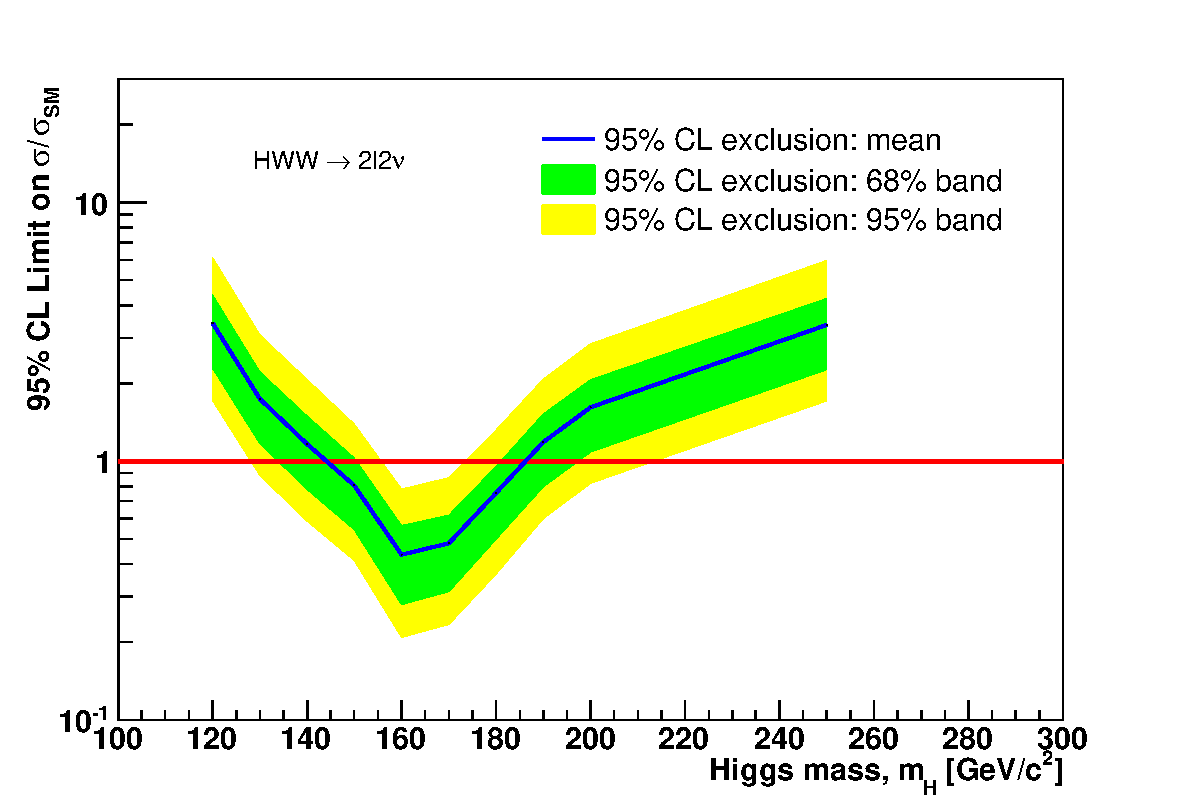
\includegraphics[width=0.9\textwidth]{figures/cut_based_limits.pdf}
   \caption{Cut based analysis expected upper limits at 95\%C.L. for 1\ifb\ of data.}
   \label{fig:cutbase_uls}
\end{center}
\end{figure}

  
%%   \clearpage

\section{Data Results with \intlumi}
%%   \label{sec:dataresults}
%%   We perform the analysis on a dataset corresponding to $1.1\pm0.1\ifb$ integrated luminosity.

Table~\ref{tab:zzselection_all} shows the number of events observed in 
data, comparing to the expected background contribution at the \zz 
preselection level. The background estimation was discussed at Section~\ref{sec:backgrounds}. 
Figure~\ref{fig:zz_0j_1} the distributions of key analysis variables observed in data, comparing 
to the SM expectations from simulation in the 0-jet bin final state.  
Tables~\ref{tab:yield_hzz250}-\ref{tab:yield_hzz400} shows the equivalent results 
applying the $\hzz$ ($m_{H}=250,300,400\GeVcc$) selections~\ref{sec:signal_selection}. 
The details of the events counts can also be found in ~\ref{app:yield1fbdetail}. 


%%%%%%%%
\begin{table}[!ht]
\begin{center}
\begin{tabular} {c|c|c|cccccc}
\hline
  & data & all bkg. & $\dyll$ & $\ZZ$ & $\WZ$ & $WW$ & $\ttbar+tW$ & $\Wjets$  \\
\hline
\multicolumn{9}{c} {0 Jet Bin} \\
\hline
 $\mu\mu$ &  39 & $43.4\pm0.9$ & $8.2\pm0.1$ & $14.5\pm0.3$ & $7.1\pm0.3$ & $11.6\pm0.4$ & $2.1\pm0.7$ & $0.0$ \\
 $ee$     &  31 & $31.7\pm0.8$ & $8.2\pm0.1$ & $9.7\pm0.2$  & $4.0\pm0.2$ & $7.5\pm0.3$ & $1.0\pm0.3$ & $1.3\pm0.6$ \\
\hline
\multicolumn{9}{c} {1 Jet Bin} \\
\hline
 $\mu\mu$ &  21 & $22.6\pm0.8$ & $8.8\pm0.1$ & $3.7\pm0.1$ & $3.7\pm0.2$ &  $3.3\pm0.2$ & $3.1\pm0.7$ & $0.0$  \\
 $ee$     &  18 & $19.6\pm0.9$ & $8.8\pm0.1$ & $2.6\pm0.1$ & $2.5\pm0.2$ & $2.2\pm0.2$ & $3.6\pm0.8$ & $0.0$ \\
\hline
\end{tabular}
\caption{Expected number of signal and background events from the data-driven methods for an 
  integrated luminosity of \intlumi  after applying the $\ZZ$ selection requirements. 
Only statistical uncertaities are reported. }
   \label{tab:zzselection_all}
  \end{center}
\end{table}
%%%%%%%%

%%%%%%%%
%\begin{table}[!ht]
%\begin{center}
%\begin{tabular} {c|c|c|c|ccccc}
%\hline
%  & data & $HZZ$(200) & all bkg. & $\dyll$ & $\ZZ$ & $\WZ$ & $WW$ & $\ttbar+tW$ \\
%\hline
%\multicolumn{9}{c} {0 Jet Bin} \\
%\hline
% $\mu\mu$ &  12 & $0.12\pm0.01$ & $13.9\pm0.4$ & $3.34\pm0.04$ & $3.1\pm0.1$ & $2.1\pm0.2$ & $4.8\pm0.2$ & $0.5\pm0.3$ \\
% $ee$     &  14 & $0.07\pm0.01$ & $9.9\pm0.3$  & $3.34\pm0.04$ & $2.0\pm0.1$ & $1.2\pm0.1$ & $3.1\pm0.2$ & $0.2\pm0.2$ \\
%\hline
%\multicolumn{9}{c} {1 Jet Bin} \\
%\hline
% $\mu\mu$ &  0 & $0.02\pm0.00$ & $0.34\pm0.10$ & $0.12\pm0.01$ & $0.02\pm0.01$ & $0.01\pm0.01$ & $0.07\pm0.03$ & $0.13\pm0.09$ \\
% $ee$     &  0 & $0.01\pm0.00$ & $0.20\pm0.03$ & $0.12\pm0.01$ & $0.01\pm0.01$ & $0.02\pm0.01$ & $0.05\pm0.02$ & $0.0$ \\
%\hline
%\end{tabular}
%\caption{Expected number of signal and background events from the data-driven methods for an 
%  integrated luminosity of \intlumi  after applying the $\hzz$ ($m_H=200\GeVcc$) selection requirements. 
%Only statistical uncertaities are reported. The $\Wjets$ background is neglible thus omitted in the table.}
%   \label{tab:yield_hzz200}
%  \end{center}
%\end{table}
%%%%%%%%


%%%%%%%%
\begin{table}[!ht]
\begin{center}
\begin{tabular} {c|c|c|c|ccccc}
\hline
  & data & $HZZ$(250) & all bkg. & $\dyll$ & $\ZZ$ & $\WZ$ & $WW$ & $\ttbar+tW$ \\
\hline
\multicolumn{9}{c} {0 Jet Bin} \\
\hline
 $\mu\mu$ &  20 & $2.12\pm0.04$ & $16.7\pm0.7$ & $3.4\pm0.1$ & $5.3\pm0.2$ & $2.7\pm0.2$ & $4.0\pm0.2$ & $1.4\pm0.0.6$ \\
 $ee$     &  7 & $1.57\pm0.03$ & $12.7\pm0.6$ & $3.4\pm0.1$ & $3.5\pm0.1$ & $1.6\pm0.1$ & $2.9\pm0.2$ & $0.5\pm0.2$ \\
\hline
\multicolumn{9}{c} {1 Jet Bin} \\
\hline
 $\mu\mu$ &  5 & $1.02\pm0.02$ & $9.1\pm0.6$ & $2.38\pm0.02$ & $1.4\pm0.1$ & $1.8\pm0.2$ & $1.7\pm0.1$ & $1.8\pm0.5$ \\
 $ee$     &  8 & $0.70\pm0.02$ & $8.6\pm0.8$ & $2.38\pm0.02$ & $1.1\pm0.1$ & $1.1\pm0.1$ & $1.2\pm0.1$ & $2.9\pm0.8$ \\
\hline
\end{tabular}
\caption{Expected number of signal and background events from the data-driven methods for an 
  integrated luminosity of \intlumi  after applying the $\hzz$ ($m_H=250\GeVcc$) selection requirements. 
Only statistical uncertaities are reported. The $\Wjets$ background is neglible thus omitted in the table.}
   \label{tab:yield_hzz250}
  \end{center}
%\end{table}
%%%%%%%%
%%%%%%%%
%\begin{table}[!ht]
\begin{center}
\begin{tabular} {c|c|c|c|ccccc}
\hline
  & data & $HZZ$(300) & all bkg. & $\dyll$ & $\ZZ$ & $\WZ$ & $WW$ & $\ttbar+tW$ \\
\hline
\multicolumn{9}{c} {0 Jet Bin} \\
\hline
 $\mu\mu$ &  3 & $1.67\pm0.03$ & $5.4\pm0.2$ & $0.26\pm0.03$ & $2.9\pm0.1$ & $1.3\pm0.1$ & $0.8\pm0.1$ & $0.09\pm0.0.05$ \\
 $ee$     &  4 & $1.18\pm0.02$ & $3.6\pm0.2$ & $0.26\pm0.03$ & $2.2\pm0.1$ & $0.6\pm0.1$ & $0.4\pm0.1$ & $0.14\pm0.14$ \\
\hline
\multicolumn{9}{c} {1 Jet Bin} \\
\hline
 $\mu\mu$ &  1 & $0.60\pm0.01$ & $1.3\pm0.2$ & $0.16\pm0.01$ & $0.47\pm0.05$ & $0.26\pm0.06$ & $0.14\pm0.04$ & $0.25\pm0.22$ \\
 $ee$     &  2 & $0.43\pm0.01$ & $0.9\pm0.1$ & $0.16\pm0.01$ & $0.34\pm0.04$ & $0.15\pm0.04$ & $0.13\pm0.03$ & $0.08\pm0.08$ \\
\hline
\end{tabular}
\caption{Expected number of signal and background events from the data-driven methods for an  
integrated luminosity of \intlumi  after applying the $\hzz$ ($m_H=300\GeVcc$) selection requirements. 
Only statistical uncertaities are reported. The $\Wjets$ background is neglible thus omitted in the table.}
   \label{tab:yield_hzz300}
  \end{center}
%\end{table}
%%%%%%%%
%%%%%%%%
%\begin{table}[!ht]
\begin{center}
\begin{tabular} {c|c|c|c|ccccc}
\hline
  & data & $HZZ$(400) & all bkg. & $\dyll$ & $\ZZ$ & $\WZ$ & $WW$ & $\ttbar+tW$ \\
\hline
\multicolumn{9}{c} {0 Jet Bin} \\
\hline
 $\mu\mu$ &  1 & $1.29\pm0.02$ & $2.3\pm0.1$ & $0.0$ & $1.7\pm0.1$ & $0.55\pm0.08$ & $0$ & $0$ \\
 $ee$     &  2 & $0.94\pm0.02$ & $1.4\pm0.1$ & $0.0$ & $1.1\pm0.1$ & $0.25\pm0.06$ & $0$ & $0$ \\
\hline
\multicolumn{9}{c} {1 Jet Bin} \\
\hline
 $\mu\mu$ &  2 & $0.97\pm0.02$ & $1.5\pm0.1$ & $0.43\pm0.05$ & $0.68\pm0.06$ & $0.37\pm0.07$ & $0.05\pm0.02$ & $0$ \\
 $ee$     &  3 & $0.70\pm0.01$ & $1.1\pm0.1$ & $0.43\pm0.05$ & $0.46\pm0.05$ & $0.21\pm0.05$ & $0.04\pm0.01$ & $0$ \\
\hline
\end{tabular}
\caption{Expected number of signal and background events from the data-driven methods for an 
integrated luminosity of \intlumi  after applying the $\hzz$ ($m_H=400\GeVcc$) selection requirements. 
Only statistical uncertaities are reported. The $\Wjets$ background is neglible thus omitted in the table.}
   \label{tab:yield_hzz400}
  \end{center}
\end{table}
%%%%%%%%






%%%%%%%%
\begin{figure}[!hbtp]
\begin{center}
\label{}
\includegraphics[width=.45\textwidth]{figures/preselection_njets.pdf}
\caption{Number of jets distribution observed in data corresponding to $187\pm7$~\ipb data, compared to the expected from simulation for signal and background. 
The background MC does not include any corrections, while we apply the $\pt$ reweighting correction in the higgs signal. }
\label{fig:njets_zzpresel}
\end{center}
\end{figure}
%%%%%%%%

%%%%%%%%
\begin{figure}[!hbtp]
\begin{center}
\label{fig:minmet_zzpresel}
\subfigure[0-Jet]{\label{subfig:minmet_0j}
\includegraphics[width=.3\textwidth]{figures/preselection_0jets_minmet.pdf}}
\subfigure[1-Jet]{\label{subfig:minmet_1j}
\includegraphics[width=.3\textwidth]{figures/preselection_1jet_minmet.pdf}}
\subfigure[$\geq$2 Jets]{\label{subfig:minmet_2j}
\includegraphics[width=.3\textwidth]{figures/preselection_2jets_minmet.pdf}}
\caption{Min-MET distribution after the $\ZZ$ preselection observed in data corresponding to $187\pm7$~\ipb data in 0-Jet~\subref{subfig:minmet_0j}, 1-Jet~\subref{subfig:minmet_1j} 
and 2-Jet~\subref{subfig:minmet_2j} bins, compared to the expected from simulation for signal and background. 
The background MC does not include any corrections, while we apply the $\pt$ reweighting correction in the higgs signal. }
\end{center}
\end{figure}
%%%%%%%%


%%%%%%%%
\begin{figure}[!hbtp]
\begin{center}
\label{fig:mt_zzpresel}
\subfigure[0-Jet]{\label{subfig:mt_0j}
\includegraphics[width=.3\textwidth]{figures/preselection_0jets_mt.pdf}}
\subfigure[1-Jet]{\label{subfig:mt_1j}
\includegraphics[width=.3\textwidth]{figures/preselection_1jet_mt.pdf}}
\subfigure[$\geq$2 Jets]{\label{subfig:mt_2j}
\includegraphics[width=.3\textwidth]{figures/preselection_2jets_mt.pdf}}
\caption{Transverse mass $m_T$ distribution after the $\ZZ$ preselection observed in data corresponding to $187\pm7$~\ipb data in 0-Jet~\subref{subfig:mt_0j}, 1-Jet~\subref{subfig:mt_1j} 
and 2-Jet~\subref{subfig:mt_2j} bins, compared to the expected from simulation for signal and background. 
The background MC does not include any corrections, while we apply the $\pt$ reweighting correction in the higgs signal. }
\end{center}
\end{figure}
%%%%%%%%

%%%%%%%%
\begin{figure}[!hbtp]
\begin{center}
\label{fig:mt_hzz300}
\subfigure[0-Jet]{\label{subfig:mt_0j}
\includegraphics[width=.3\textwidth]{figures/preselection_0jets_mt.pdf}}
\subfigure[1-Jet]{\label{subfig:mt_1j}
\includegraphics[width=.3\textwidth]{figures/preselection_1jet_mt.pdf}}
\subfigure[$\geq$2 Jets]{\label{subfig:mt_2j}
\includegraphics[width=.3\textwidth]{figures/preselection_2jets_mt.pdf}}
\caption{Transverse mass $m_T$ distribution after the full $\hzz$ ($m_H = 300\GeVcc$) selection observed in 
data corresponding to $187\pm7$~\ipb data in 0-Jet~\subref{subfig:mt_0j}, 1-Jet~\subref{subfig:mt_1j} 
and 2-Jet~\subref{subfig:mt_2j} bins, compared to the expected from simulation for signal and background. 
The background MC does not include any corrections, while we apply the $\pt$ reweighting correction in the higgs signal. }
\end{center}
\end{figure}
%%%%%%%%


\section{Summary}
     \label{sec:summary}
     In summary, we described an analysis to study the spin of a single narrow 
resonance at 125 GeV by the gluon fusion through the decays into $WW\to 2\ell2\nu$.  
The analysis is based on a two-dimensional templates $m_T-m_{\ell\ell}$. 
The expected sensitivity to distinguish between between SM Higgs hypothesis and 
spin 2 Graviton like resonance with minimal coupling 
$2_\text{min}^+$ is $1.7\sigma$ for \intlumiEightTeV. 
Scaling by luminosity the projected separation is about $2.0\sigma$ for 25~$\ifb$. 


%===================================================================================================
\clearpage

\vspace*{-0.2cm}
\thebibliography{12}

\bibitem{pdg}
 K. Nakamura et al. (Particle Data Group), "Review of particle physics", J. Phys.G37 , 2010.

\bibitem{Higgs1}
F. Englert and R. Brout, "Broken symmetries and the masses of gauge bosons", Phys. Rev. Lett. 13,  1964.

\bibitem{Higgs2}
P. W. Higgs, "Broken symmetry and the mass of gauge vector mesons", Phys. Rev. Lett. 13, 1964.

\bibitem{Higgs3}
Guralnik, G.S. and Hagen, C.R. and Kibble, T.W.B., "Global Conservation Laws and Massless Particles", 
Phys.Rev.Lett. 13, 1964.

\bibitem{HWW2010}
CMS Collaboration, "Title: Measurement of WW Production and Search for the Higgs Boson in 
pp Collisions at $\sqrt{s}$ = 7 TeV", arXiv:1102.5429

\bibitem{VBTFCrossSectionNote}
J. Alcaraz Maestre, \textit{et al.}, "Updated Measurements of Inclusive W and Z Cross Sections 
at $\sqrt{s}=7$ TeV", CMS AN-2010/264.

\bibitem{ggWWError}
F.~ Stoeckli, "http://indico.cern.ch/getFile.py/access?contribId=0\&resId=1\&materialId=slides\&confId=49009", 
EWK Diboson meeting of March 12 2009.

\bibitem{json}
{\small
/afs/cern.ch/cms/CAF/CMSCOMM/COMM\_DQM/certification/Collisions11/7TeV/Prompt/Cert\_160404-163869\_7TeV\_PromptReco\_Collisions11\_JSON.txt
}

\bibitem{ElIso}
A. Vartak, M. LeBourgeois, V. Sharma, "Lepton Isolation in the CMS Tracker, ECAL and HCAL", CMS AN-2010/106.

\bibitem{PVDA}
W. Erdmann, M. LeBourgeois, B. Mangano, 
https://indico.cern.ch/getFile.py/access?contribId=5\&sessionId=3\&resId=1\&materialId=slides\&confId=127127, 
note in preparation.

\bibitem{NExpHits}
B. Mangano \textit{et al.}, "Improvement in Photon Conversion Rejection Performance Using 
Advanced Tracking Tools", AN-10-283.

\bibitem{fakeLeptonNote1}
S.~Xie, \textit{et al.}", "Study of Data-Driven Methods for Estimation of Fake Lepton Backgrounds", 
CMS AN-2009/120.

\bibitem{fakeLeptonNote2}
W.~Andrews, \textit{et al.}, "Fake Rates for dilepton Analyses", CMS AN-2010/257.

\bibitem{fakeLeptonBkgSpillage1}
 F. Golf, D. Evans, J. Mulmenstadt  \textit{et al.}, ``Expectations for observation of top quark pair production in the dilepton final state with the early CMS data'', CMS AN-2009/050.

\bibitem{dyestnote}
W. Andrews, et al., “A Method to Measure the Contribution of $\dyll$ to a di-lepton+ MET Selection”, CMS AN-2009/023 (2009).

\bibitem{jes}
CMS Collaboration, "Jet Energy Calibration with Photon+Jet Events", PAS JME-09-004.

\bibitem{jetpas}
CMS Collaboration, "Jet Performance in pp Collisions at $\sqrt{s}=7 \rm\ TeV$", PAS JME-10-003.

\bibitem{btag}
CMS collaboration, "Commissioning of b-jet identification with pp collisions at $\sqrt{s}=7~\TeV$, BTV-10-001.

\bibitem{antikt}
Cacciari, Matteo and Salam, Gavin P. and Soyez, Gregory, "The anti-$k_t$ jet clustering 
algorithm", JHEP 04,  2008.

\bibitem{ConversionNote}
W.~Andrews, \textit{et al.}, "Study of photon conversion rejection at CMS", CMS AN-2009/159.

\bibitem{tmva}
A. Hoecker, \textit{et al.}, "TMVA - Toolkit for Multivariate Data Analysis", arXiv:physics/0703039, 2007.

\bibitem{XS}
CMS Generator group, Standard Model Cross Sections for CMS at 7 TeV, 2010.

\bibitem{PDF4LHC}
PDF4LHC Working Group, 
{\tt http://www.hep.ucl.ac.uk/pdf4lhc/PDF4LHCrecom.pdf}

\bibitem{Nadolsky:2008zw}
Nadolsky, Pavel M. and others, "Implications of CTEQ global analysis for 
collider observables", Phys. Rev. D78 2008.

\bibitem{Martin:2009iq}
Martin, A. D. and Stirling, W. J. and Thorne, R. S. and Watt, G., "Parton 
distributions for the LHC, Eur. Phys. J. C63 2009.

\bibitem{Ball:2010de}
Ball, Richard D. and others, "A first unbiased global NLO determination 
of parton distributions and their uncertainties", arXiv 1002.4407.

\bibitem{bayesian}
A. O'Hagan and J.J. Forster, "Bayesian Inference", Kendall's Advanced Theory of Statistics, 
Arnold, London, 2B, 2004.

\bibitem{ref:tagprobe_mit_w}
G. Bauer {\it et. al.}, "Lepton ef?iencies for the inclusive W cross section measurement with 36.1pb$^{-1}$", AN2011/097

\bibitem{ref:tagprobe_snt_top}
W. Andrews {\it et. al.}, "Uncertainties on the Lepton Selection Efficiency for t$t\bar{t}$ Cross Section Analysis", AN2010/274

\bibitem{LHCHiggsCrossSectionWorkingGroup:2011ti}
LHC Higgs Cross Section Working Group, "Handbook of LHC Higgs Cross Sections: 
Inclusive Observables", CERN-2011-002, 2011.

\bibitem{PFMET} 
CMS Collaboration, ``CMS MET Performance in Events Containing Electroweak Bosons from pp Collisions at $\sqrt{s}=7$ TeV'', CMS PAS JME-2010-005 (2010)


\bibitem{trkMET} 
Marco Zanetti, ``MET with PU in $\hww\to2\ell$'', https://indico.cern.ch/conferenceDisplay.py?confId=131580
Benjamin Hooberman, ``MET with PU in MC and First 2011 Data'', https://indico.cern.ch/contributionDisplay.py?contribId=5\&confId=132579. 


\bibitem{lands}
Mingshui Chen and Andrey Korytov, https://mschen.web.cern.ch/mschen/lands/

\bibitem{MCFMHiggsProduction}
J. Campbell, R.K. Ellis, G. Zanderighi, ``Next-to-Leading order Higgs + 2 jet production via gluon fusion.'', JHEP 0610:028 (2006), hep-ph/0608194

%===================================================================================================
\newpage 
\appendix
\appendixpage
\section{Data Samples}
  \label{app:datasets}
  %UPDATEME%
The datasets used for this analysis are summarized in 
Tables~\ref{tab:DatasetsData} and~\ref{tab:DatasetsMC} for data and Monte 
Carlo, respectively. The total integrated luminosity is \intlumiEightTeV. 
We used the official good run list~\cite{json}. For Monte Carlo simulation 
we use madgraph when possible, but different generators such as Pythia and Powheg~\cite{powheg} 
are also used.  For $gg \to \WW$ a dedicated generator is used. For \wz\ and \zz\
processes we use Pythia, since MadGraph samples are mixed with $\WW$ in
a single $VV$ sample, which is difficult to use properly.

\begin{table}[!ht]
\begin{center}
\begin{tabular}{|c|c|}
\hline
 Dataset Description                   &   Dataset Name   \\
\hline \hline
\multirow{2}{*}{MuEl PromptReco}   		&  /MuEG/Run2012A-PromptReco-v1/AOD   \\
            							&  /MuEG/Run2012B-PromptReco-v1/AOD   \\
\multirow{2}{*}{DiMuon PromptReco}     	&  /DoubleMu/Run2012A-PromptReco-v1/AOD   \\
          								&  /DoubleMu/Run2012B-PromptReco-v1/AOD   \\
\multirow{2}{*}{DiElectron PromptReco} 	&  /DoubleElectron/Run2012A-PromptReco-v1/AOD   \\
      									&  /DoubleElectron/Run2012B-PromptReco-v1/AOD   \\
\multirow{2}{*}{SingleMuon PromptReco}  &  /SingleMu/Run2012A-PromptReco-v1/AOD   \\
      									&  /SingleMu/Run2012B-PromptReco-v1/AOD   \\
\multirow{2}{*}{SingleElectron PromptReco} 	&  /SingleElectron/Run2012A-PromptReco-v1/AOD   \\
      										&  /SingleElectron/Run2012B-PromptReco-v1/AOD   \\
\hline
\end{tabular}
\caption{Summary of data datasets used.\label{tab:DatasetsData}}
\end{center}
\end{table}

\begin{table}[!ht]
\begin{center}
{\footnotesize
\begin{tabular}{|c|c|c|}
\hline
\multicolumn{3}{|c|}{With Pileup: Processed dataset name is always} \\
\multicolumn{3}{|c|}{/Summer12-PU\_S7\_START52\_V9-v*/AODSIM} \\
\hline
 Dataset Description              		&   Primary Dataset Name   & cross-section (pb)\\
\hline
$\ttbar$                              	&   /TTJets\_TuneZ2star\_8TeV-madgraph-tauola                          	& 	225.2 	\\
tW                  	 	 			&   /T\_tW-channel-DR\_TuneZ2star\_8TeV-powheg-tauola                  	&  	11.18 	\\
$\bar{\textrm{t}}$W                   	&   /Tbar\_tW-channel-DR\_TuneZ2star\_8TeV-powheg-tauola               	&  	11.18 	\\
gg $\rightarrow WW \to 2l 2\nu$         &   /GluGluToWWTo4L\_TuneZ2star\_8TeV-gg2ww-pythia6                     &   1.74	\\
qq $\rightarrow WW$                  	&   /WWJetsTo2L2Nu\_TuneZ2star\_8TeV-madgraph-tauola                    &  	5.81  	\\
WZ                               	 	&   /WZ\_TuneZ2star\_8TeV\_pythia6\_tauola                        		&  	22.45 	\\
Z[10-50] 	  	 						&   /DYJetsToLL\_M-10To50filter\_8TeV-madgraph                   		&  	860.5 	\\
Z[50-inf] 	  	 						&   /DYJetsToLL\_M-50\_TuneZ2Star\_8TeV-madgraph-tarball           		&  	3532.8 	\\
ZZ $\rightarrow 2l 2\nu$    	 		& 	/ZZJetsTo2L2Nu\_TuneZ2star\_8TeV-madgraph-tauola                    &   0.365	\\
ZZ $\rightarrow 2l 2q$    	 			&   /ZZJetsTo2L2Q\_TuneZ2star\_8TeV-madgraph-tauola                     &   1.28	\\
ZZ $\rightarrow 4l$    	 				&   /ZZJetsTo4L\_TuneZ2star\_8TeV-madgraph-tauola                       &   0.0921	\\
$gg \to H \to WW \to 2l 2\nu$         	&   /GluGluToHToWWTo2LAndTau2Nu\_M-*\_8TeV-powheg-pythia6             	& 	vary 	\\
$qqH,~H \to WW \to 2l 2\nu$           	&   /VBF\_HToWWTo2LAndTau2Nu\_M-*\_8TeV-powheg-pythia6                 	& 	vary 	\\
$WH/ZH/\ttbar H,~H\to WW$              	&   /WH\_ZH\_TTH\_HToWW\_M-*\_8TeV-pythia6                            	& 	vary 	\\
\hline
\hline
\end{tabular}
}
\caption{Summary of Monte Carlo datasets used.\label{tab:DatasetsMC}. The cross sections for a SM Higgs boson
is taken from the LHC Higgs cross-section working group~\cite{LHCHiggsCrossSectionWorkingGroup:2011ti}}
\end{center}
\end{table}

Since some portion of data datasets were not processed, 
we use a json excluding missing events~\cite{json}. 
Last year we adjusted Higgs $\pt$ spectrum because 
the spectrum in the simulation (POWHEG 2.0) was harder than the one 
in the most precise calculation to NNLO with resummation to NNLL order.
In the new version of Powheg (POWHEG 2.1), this problem has been mostly resolved,
thus we do not apply any corrections for Higss $\pt$.

  
%%   \section{Primary Vertex Reweighting}
%%      \label{app:vertex_reweight}
%%      To make sure the simulation reproduces the data, we reweight the number of
primary verteces in the simulation to match the distribution observed in the 
data, after requiring that the event has two leptons passing offline
lepton selection. The number of Primary verteces in data and simulation before and
after applying the reweighting procedure in dilepton events is shown in
Figure~\ref{fig:nvert_zll}. The weight factor applied to the simulation 
depending on the number of primary verteces is listed in 
Table~\ref{tab:nvert_zll}.

\begin{figure}[!htbp]
\begin{center}
   \subfigure[]{\includegraphics[width=0.49\textwidth]{figures/nvert_zll_noreweight.pdf}}
   \subfigure[]{\includegraphics[width=0.49\textwidth]{figures/nvert_zll_reweight.pdf}} 
\caption{Number of Primary verteces in data and simulation before (a) and
after (b) applying the reweighting procedure in dilepton events.}
\label{fig:nvert_zll}
\end{center}
\end{figure}

\begin{table}[!ht]
\begin{center}
\begin{tabular}{|c|c|}
\hline
 $N_{vertex}$ &   weight   \\
\hline
\hline
 1        & 0.215 \\
 2        & 0.742 \\
 3        & 1.414 \\
 4        & 1.780 \\
 5        & 1.796 \\
 6        & 1.486 \\
 7        & 1.092 \\
 8        & 0.752 \\
 9        & 0.556 \\
10        & 0.369 \\
11        & 0.255 \\
12        & 0.166 \\
13        & 0.114 \\
14        & 0.106 \\
15        & 0.056 \\
$\geq$16  & 0.010 \\
\hline
\end{tabular}
\caption{Weight factor applied to the simulation depending on the number of
primary verteces.\label{tab:nvert_zll}}
\end{center}
\end{table}

%%   \clearpage
%%   \section{Electron Selection Optimization}
%%      \label{app:els}
%%      \subsection{Introduction}
The published $H\rightarrow WW\rightarrow 2\ell 2\nu$ analysis of 2010 was based on the following electron selection:
\begin{itemize}
\item identification: VBTF80;
\item isolation: relIso$<$0.10, where relIso is the sum of contributions from tracks, ECAL, and HCAL in a cone of R=0.3 around the electron, 
divided by the electron $p_T$; in the barrel the ECAL contribution has a pedestal subtraction of 1 GeV;
\item impact parameter: transverse longitudinal parameter w.r.t. the primary vertex $<0.02$ cm and longitudinal i.p. $<$ 0.2 cm;
\item conversion rejection: 0 missing inner expected hits and partner track veto (distance $<$0.02 cm, $\Delta \cot \theta <$0.02).
\end{itemize}
Before the 2011 data taking we wanted to review the selection and check if there is anything better available.

This process is divided into two steps: we review the available selections for high $p_T$ electrons ($>$20 GeV) and then, 
we look for improvement for a possible extension at low $p_T$.

The choice of the optimal selection is based on the analysis results after all cuts, 
but we cross-check the performance in terms of efficiency of fake vs good electrons.
Also, we checked the performance in 2011 data and with high PU conditions.

\subsection{Procedure Definition}
The performance of the tested algorithms are evaluated using three figures of merit (FOM):
\begin{itemize}
\item FOM1: $S/B$, the signal to background ratio;
\item FOM2: $S/\sqrt{S+B}$, the statistical significance;
\item FOM3: $S/\sqrt{S+B+(0.35 \cdot B)^2}$, the significance including a 35\% systematic uncertainty on the background;
\end{itemize}
where S and B are the total signal and background yields for an integrated luminosity of 1/fb and evaluated in the 2010 
$H\rightarrow WW\rightarrow 2\ell 2\nu$, $m_H=130$ GeV analysis signal region:
$\Delta\phi < 60$, 12$< m_{ll} <$45 GeV, projected Met$>$35 GeV (20 GeV for $\mu$-e final state), jet and top veto.
In this exercise we consider the final states where the trailing lepton is an electron ($\mu$-e and e-e).
The choice of 35\% in the FOM3 definition is somewhat arbitrary; the idea is to pick a conservative value on the background systematic uncertainty, 
as opposed to FOM2 where the assumption of negligible systematic uncertainty is too optimistic.

Yields are evaluated according to a simple model that treats good and fake electrons separately.
Real electrons are well modeled by simulation and thus we can rely on efficiency estimates from Monte Carlo; 
we use the electron efficiency from the signal sample to scale the signal and non-fake background yields.
Fake and non-prompt electrons, instead, can't be studied on simulation since their physics origin is difficult to parametrize and because
the available sample has low statistics. 
Therefore, we predict the fake background yield from data with the following procedure: 
first, we take as baseline the prediction from 2010 data scaled to 1/fb (using the fake rate method for 2010 analysis electron selection); 
then for each of the tested selections, we calculate the efficiency per fake electron from data and use this efficiency to scale the baseline prediction.

Fake electrons from data are selected from the EG2010A sample requiring HLT\_Ele10\_SW\_L1R and rejecting electrons from W and Z with the following cuts:
Met$<$20 GeV, $m_T(e, Met)<$20 GeV and, for event with two electrons, $|m_{ee}-m_Z|>$15 GeV. 
The selected sample includes about 6500 electrons passing the 2010 analysis selection.

Yields and efficiencies are computed in three bins both in $p_T$ ($[10,15],[15,20],[20,\infty]$, values in GeV) 
and in $|\eta|$ ($[0,1.0],[1.0,1.5],[1.5,2.5]$). 
Tables~\ref{tab:fakeBaseline}-\ref{tab:hww130yieds} report the baseline prediction from 2010 fake data and non-fake background and signal from MC.
For 10$<p_T<$15 GeV the background contribution from fakes is dominant, while at higher $p_T$ it is comparable or smaller than the sum of the other backgrounds.

\begin{table}[!ht]
\begin{center}
\begin{tabular}{|c|ccc|c|} \hline
 & $0.0<|\eta|<1.0$ & $1.0<|\eta|<1.5$ & $1.5<|\eta|<2.5$ & All $\eta$ \\ \hline
10$<p_T<$15 & 9.11 & 3.41 & 1.18 & 13.70 \\
15$<p_T<$20 & 3.22 & 0.00 & 0.93 & 4.15 \\
$p_T>$20 & 1.24 & 2.85 & 1.05 & 5.14 \\  \hline
All $p_T$ & 13.57 & 6.26 & 3.16 & 22.99 \\ \hline
\end{tabular}
\caption{Fake rate prediction for $\mu$-e and e-e final states from 2010 data. 
The electron selection is the same as in 2010 analysis and the results is scaled to 1/fb.
The total uncertainty is of the order of 50\%.
\label{tab:fakeBaseline}}
\end{center}
\end{table}

\begin{table}[!ht]
\begin{center}
\begin{tabular}{|c|ccc|c|} \hline
 & $0.0<|\eta|<1.0$ & $1.0<|\eta|<1.5$ & $1.5<|\eta|<2.5$ & All $\eta$ \\ \hline
10$<p_T<$15 & 2.15 & 0.81 & 1.03 & 4.00 \\
15$<p_T<$20 & 4.18 & 1.42 & 1.26 & 6.87 \\
$p_T>$20    & 10.26& 4.89 & 3.57 & 18.71\\  \hline
All $p_T$   & 16.59& 7.12 & 5.86 & 29.58 \\ \hline
\end{tabular}
\caption{MC yield prediction for non-fake electron backgrounds ($\mu$-e and e-e final states). 
The electron selection is the same as in 2010 analysis and the results is scaled to 1/fb.
\label{tab:nonfakeyieds}}
\end{center}
\end{table}

\begin{table}[!ht]
\begin{center}
\begin{tabular}{|c|ccc|c|} \hline
 & $0.0<|\eta|<1.0$ & $1.0<|\eta|<1.5$ & $1.5<|\eta|<2.5$ & All $\eta$ \\ \hline
10$<p_T<$15 & 0.79 & 0.22 & 0.18 & 1.19 \\
15$<p_T<$20 & 1.09 & 0.37 & 0.32 & 1.78 \\
$p_T>$20    & 2.18 & 0.69 & 0.54 & 3.41 \\  \hline
All $p_T$   & 4.06 & 1.28 & 1.04 & 6.38 \\ \hline
\end{tabular}
\caption{MC yield prediction for $H\rightarrow WW$ sample ($m_H=130$ GeV) ($\mu$-e and e-e final states). 
The electron selection is the same as in 2010 analysis and the results is scaled to 1/fb.
\label{tab:hww130yieds}}
\end{center}
\end{table}

We optimize the electron identification, isolation and impact parameter selections separately, changing one cut at a time.
We checked that, using different isolation algorithms as baseline, the optimal identification working point is the same.
Therefore, we use the 2010 selection as a baseline for the optimization process.

\subsection{Electron Identification}

We compared the performance of several electron identification algorithms available in the collaboration.
They can be grouped in three sets:
\begin{itemize}
\item Simple Cuts (VBTF: 4 variables, separate cuts for barrel/endcap): 
  \begin{itemize}
  \item VBTF85
  \item VBTF80 
  \item VBTF70
  \end{itemize}
\item Multivariate techniques, exploiting correlations between variables (MVA): 
  \begin{itemize}
  \item MVA05: particle flow MVA output$>$0.5 
  \item MVA07: particle flow MVA output$>$0.7 
  \item LHT: Likelihood ID, tight WP\footnote{UserCode/emanuele/EgammaAnalysisTools, tag ``edm-Feb2011'' and latest PDFs: \\
http://indico.cern.ch/getFile.py/access?contribId=4\&resId=0\&materialId=slides\&confId=127254.}
  \end{itemize}
\item Categorized cuts (CIC: advanced cut based tuning in multiple categories)\footnote{CIC version V06 with data driven tuning \\
http://cmssw.cvs.cern.ch/cgi-bin/cmssw.cgi/CMSSW/RecoEgamma/ElectronIdentification/python/\\
cutsInCategoriesElectronIdentificationV06\_DataTuning\_cfi.py?view=log.}: 
  \begin{itemize}
  \item CICST: CIC SuperTight ID 
  \item CICHT2: CIC HyperTight v2 ID
  \item CICHT4: CIC HyperTight v4 ID
  \end{itemize}
\end{itemize}

\subsubsection{Results for $p_T>$20 $\GeVc$}

The first step is the definition of a baseline cut at high $p_T$. 
We verify the identification performance by comparing the cut efficiency on fake electrons from data and on signal electrons on MC.
Figure~\ref{subfig:idEffic_gt20} shows that the MVA curve has worse rejection power than CIC, while the VBTF and CIC curves cross.
This result can be interpreted in terms of analysis performance by looking at the FOM's for $p_{T,max}>$20 GeV and $p_{T,min}>$20 GeV
(Figs.~\ref{subfig:id_hww130_fom1_pt20}-\ref{subfig:id_hww130_fom3_pt20}). 
No algorithm provides the best results for all FOM's; however, it is clear that MVA is slightly worse, while VBTF and CIC are comparable.
Therefore, we think that it is safe to continue with the VBTF approach as baseline for the analysis:
reasonable working points for the $m_H=$130 GeV analysis are VBTF80 and VBTF70. 
However, VBTF70 might be too tight for mass values higher than $m_H=$130 GeV where the $p_T$ spectrum of the signal leptons 
is harder and the fake background less important.
 
\begin{figure}[!hbtp]
\subfigure[]{
\centering
\label{subfig:idEffic_gt20}
\includegraphics[width=.45\textwidth]{figures/idEffic_gt20.png}}
\subfigure[]{
\centering
\label{subfig:id_hww130_fom1_pt20}
\includegraphics[width=.45\textwidth]{figures/id_hww130_fom1_pt20.png}}\\
\subfigure[]{
\centering
\label{subfig:id_hww130_fom2_pt20}
\includegraphics[width=.45\textwidth]{figures/id_hww130_fom2_pt20.png}}
\subfigure[]{
\centering
\label{subfig:id_hww130_fom3_pt20}
\includegraphics[width=.45\textwidth]{figures/id_hww130_fom3_pt20.png}}\\
\caption{Relative ID efficiency (w.r.t. VBTF80) on fake electrons from data vs good electrons from signal MC \subref{subfig:idEffic_gt20};
FOM1, FOM2 and FOM3 \subref{subfig:id_hww130_fom1_pt20},\subref{subfig:id_hww130_fom2_pt20},\subref{subfig:id_hww130_fom3_pt20}. 
Electrons have $p_T>$20 GeV; the 2010 selection is used as a baseline, the ID cut is varied only.}
\label{fig:idpt20}
\end{figure}

\subsubsection{Additional Requirements for $p_T<$20 $\GeVc$}

The cut based approach is a reasonable choice as a baseline for high $p_T$, but at low $p_T$ fakes dominate and more rejection power might be needed; 
Therefore, we propose an additional cut to tighten the selection at low $p_T$.

The idea is to introduce a simple categorization based on fbrem, $\eta$ and $E/p$ (Figure~\ref{fig:smurfcuts}).
When a particle passing electron ID criteria has a high fbrem (fbrem$>$0.15) we are confident it is an electron and we keep it.
Because of the high tracker material budget, at $|\eta|>$1 almost all signal electron radiate and thus we reject all electron candidates with fbrem$<$0.15.
At $|\eta|<$1, instead, there is less tracker material and electrons with low fbrem are frequent: in this region we keep electrons with $E/p>$0.95.

In summary, we apply the following additional cut for electrons with $p_T<$20 GeV:
\begin{equation}
fbrem>0.15~OR~(|\eta|<1~AND~E/p>0.95)
\end{equation}
In the following, we call VBTF80+ (VBTF70+) the VBTF80 (VBTF70) selection added of the proposed cut above.

\begin{figure}[!hbtp]
\subfigure[]{
\centering
\label{subfig:Data_fbrem_eta}
\includegraphics[width=.45\textwidth]{figures/Data_fbrem_eta.png}}
\subfigure[]{
\centering
\label{subfig:Data_eOverPIn_bar}
\includegraphics[width=.45\textwidth]{figures/Data_eOverPIn_bar.png}}\\
\subfigure[]{
\centering
\label{subfig:HWW130_fbrem_eta}
\includegraphics[width=.45\textwidth]{figures/HWW130_fbrem_eta.png}}
\subfigure[]{
\centering
\label{subfig:HWW130_eOverPIn_bar}
\includegraphics[width=.45\textwidth]{figures/HWW130_eOverPIn_bar.png}}\\
\caption{fbrem vs $|\eta|$ (left) and $E/p$ (right) distributions for fake electrons in data (up) and good electrons in signal MC (down).}
\label{fig:smurfcuts}
\end{figure}

\subsubsection{Results for 15$<p_T<$20 $\GeVc$}

The efficiency plot (Figure~\ref{subfig:idEffic_15pt20}) shows that, also in this $p_T$ range, the CIC curve is better than MVA and
the VBTF curve again goes across. It is worth noting that the kink in the last two points of the VBTF curve is due to the additional cuts.
The FOM's for $p_{T,max}>$20 GeV and $p_{T,min}>$15 GeV are shown in Figs.~\ref{subfig:id_hww130_fom1_pt15}-\ref{subfig:id_hww130_fom3_pt15}:
all FOM's are improved w.r.t. to the corresponding values for $p_{T,min}>$20 GeV and an additional improvement is gained using VBTF+.

\begin{figure}[!hbtp]
\subfigure[]{
\centering
\label{subfig:idEffic_15pt20}
\includegraphics[width=.45\textwidth]{figures/idEffic_15pt20.png}}
\subfigure[]{
\centering
\label{subfig:id_hww130_fom1_pt15}
\includegraphics[width=.45\textwidth]{figures/id_hww130_fom1_pt15.png}}\\
\subfigure[]{
\centering
\label{subfig:id_hww130_fom2_pt15}
\includegraphics[width=.45\textwidth]{figures/id_hww130_fom2_pt15.png}}
\subfigure[]{
\centering
\label{subfig:id_hww130_fom3_pt15}
\includegraphics[width=.45\textwidth]{figures/id_hww130_fom3_pt15.png}}\\
\caption{Relative ID efficiency (w.r.t. VBTF80) on fake electrons from data vs good electrons from signal MC \subref{subfig:idEffic_15pt20} 
(15$<p_T<$20 GeV);
FOM1, FOM2 and FOM3 \subref{subfig:id_hww130_fom1_pt15},\subref{subfig:id_hww130_fom2_pt15},\subref{subfig:id_hww130_fom3_pt15} for analysis with  
$p_{T,min}>$15 GeV; the 2010 selection is used as a baseline, the ID cut is varied only.}
\label{fig:idpt15}
\end{figure}

\subsubsection{Results for 10$<p_T<$15 $\GeVc$}

Again, the VBTF+ cuts significantly improve the ID performance (Figure~\ref{subfig:idEffic_10pt15}).
However, despite VBTF+ brings a large relative improvement, the FOM's for $p_{T,max}>$20 GeV and $p_{T,min}>$10 GeV 
(Figs.~\ref{subfig:id_hww130_fom1_pt10}-\ref{subfig:id_hww130_fom3_pt10}) do not show an overall enhancement w.r.t. $p_{T,min}>$15 GeV.

\begin{figure}[!hbtp]
\subfigure[]{
\centering
\label{subfig:idEffic_10pt15}
\includegraphics[width=.45\textwidth]{figures/idEffic_10pt15.png}}
\subfigure[]{
\centering
\label{subfig:id_hww130_fom1_pt10}
\includegraphics[width=.45\textwidth]{figures/id_hww130_fom1_pt10.png}}\\
\subfigure[]{
\centering
\label{subfig:id_hww130_fom2_pt10}
\includegraphics[width=.45\textwidth]{figures/id_hww130_fom2_pt10.png}}
\subfigure[]{
\centering
\label{subfig:id_hww130_fom3_pt10}
\includegraphics[width=.45\textwidth]{figures/id_hww130_fom3_pt10.png}}\\
\caption{Relative ID efficiency (w.r.t. VBTF80) on fake electrons from data vs good electrons from signal MC \subref{subfig:idEffic_10pt15} 
(10$<p_T<$15 GeV);
FOM1, FOM2 and FOM3 \subref{subfig:id_hww130_fom1_pt10},\subref{subfig:id_hww130_fom2_pt10},\subref{subfig:id_hww130_fom3_pt10} for analysis with  
$p_{T,min}>$10 GeV; the 2010 selection is used as a baseline, the ID cut is varied only.}
\label{fig:idpt10}
\end{figure}

\subsubsection{Conclusions}

In summary, the cut based approach for electron ID is optimal for the $H\rightarrow WW$ analysis and the proposed additional cuts add more rejection power 
for $p_T<$20 GeV. Lowering the $p_{T,min}$ cut to 15 GeV improves the analysis, while at 10 GeV there is no clear benefit. 
Thus, we choose VBTF80 for $p_T>$20 GeV and VBTF70+ for 15$<p_T<$20 GeV.

\subsection{Electron Isolation}

The 2010 analysis used relIso$<$0.10.
Given that the ID optimization suggests to lower the  $p_{T,min}$ cut to 15 GeV, we wanted to review if tightening the isolation cut further 
would improve the performance of the analysis.
Within the cut based approach, we can tighten the cut in three ways: lowering the cut value, increasing the cone size, and removing the pedestal subtraction.
In the following tests, we call (tight) sliding isolation the following set of cuts: 
\begin{itemize}
\item relIso$<$0.1 (0.1) for $p_T>$20 GeV
\item relIso$<$0.07 (0.03) for 15$<p_T<$20 GeV
\item relIso$<$0.05 (0.01) for 10$<p_T<$15 GeV
\end{itemize}
and we will test it with cone size 0.3 and cone size 0.4 with and without pedestal subtraction.
CIC isolation uses cone size 0.3 for the tracker and 0.4 for the calorimeters and does not apply pedestal subtracion; cut values are optimized for various categories.
Results are summarized in Figure~\ref{fig:isopt15}. 
The efficiency plot shows that the cut based approach is basically one single curve covering the whole range and it is slightly worse than CIC; 
however, there is not a clear advantage in using tighter isolation approaches since FOM1 and FOM3 slightly improve, while FOM2 worsens. 
Therefore, we choose to stick to the relIso$<$0.10 cut. This exercise will be repeated with 2011 fake data.

\begin{figure}[!hbtp]
\subfigure[]{
\centering
\label{subfig:isoEffic_15pt20}
\includegraphics[width=.45\textwidth]{figures/isoEffic_15pt20.png}}
\subfigure[]{
\centering
\label{subfig:iso_hww130_fom1_pt15}
\includegraphics[width=.45\textwidth]{figures/iso_hww130_fom1_pt15.png}}\\
\subfigure[]{
\centering
\label{subfig:iso_hww130_fom2_pt15}
\includegraphics[width=.45\textwidth]{figures/iso_hww130_fom2_pt15.png}}
\subfigure[]{
\centering
\label{subfig:iso_hww130_fom3_pt15}
\includegraphics[width=.45\textwidth]{figures/iso_hww130_fom3_pt15.png}}\\
\caption{Relative isolation efficiency (w.r.t. relIso) on fake electrons from data vs good electrons from signal MC \subref{subfig:isoEffic_15pt20} 
(15$<p_T<$20 GeV);
FOM1, FOM2 and FOM3 \subref{subfig:iso_hww130_fom1_pt15},\subref{subfig:iso_hww130_fom2_pt15},\subref{subfig:iso_hww130_fom3_pt15} for analysis with  
$p_{T,min}>$15 GeV; the 2010 selection is used as a baseline, the isolation cut is varied only.}
\label{fig:isopt15}
\end{figure}

\subsection{Impact Parameter}

The same test have been performed varying the impact parameter (IP) cut.
We have tested the folowing approaches:
\begin{itemize}
\item 2D impact parameter cut
\item 2D impact parameter significance cut
\item 3D impact parameter cut
\item 3D impact parameter significance cut
\end{itemize}
where the impact parameter is computed with respect to the signal primary vertex (PV) reconstructed with the standard vertexing 
algorithm (\emph{offlinePrimaryVertex}).
Figure~\ref{subfig:ipEffic_15pt20} shows that, for 15$<p_T<$20 the best performance are obtained with the 2D impact parameter plain cut.
The FOM's show very little difference between the various approaches (Figs.~\ref{fig:ippt15}\subref{subfig:ip_hww130_fom1_pt15}-\subref{subfig:ip_hww130_fom3_pt15}).
We choose a 2D impact parameter cut value of 0.02 cm.

\begin{figure}[!hbtp]
\subfigure[]{
\centering
\label{subfig:ipEffic_15pt20}
\includegraphics[width=.45\textwidth]{figures/ipEffic_lt20.png}}
\subfigure[]{
\centering
\label{subfig:ip_hww130_fom1_pt15}
\includegraphics[width=.45\textwidth]{figures/ip_hww130_fom1_pt15.png}}\\
\subfigure[]{
\centering
\label{subfig:ip_hww130_fom2_pt15}
\includegraphics[width=.45\textwidth]{figures/ip_hww130_fom2_pt15.png}}
\subfigure[]{
\centering
\label{subfig:ip_hww130_fom3_pt15}
\includegraphics[width=.45\textwidth]{figures/ip_hww130_fom3_pt15.png}}\\
\caption{Relative IP efficiency (w.r.t. d0(PV)$<$0.02) on fake electrons from data vs good electrons from signal MC \subref{subfig:ipEffic_15pt20} 
(15$<p_T<$20 GeV);
FOM1, FOM2 and FOM3 \subref{subfig:ip_hww130_fom1_pt15},\subref{subfig:ip_hww130_fom2_pt15},\subref{subfig:ip_hww130_fom3_pt15} for analysis with  
$p_{T,min}>$15 GeV; the 2010 selection is used as a baseline, the d0 cut is varied only.}
\label{fig:ippt15}
\end{figure}

\subsection{Studies with Data}

We measured the efficiency of the additional proposed cuts on 2010 data using the tag and probe method.
We use a N-1 approach, where we choose di-electron events with 76$<M_{ee}<$106 GeV and the denominator is given by electrons passing 2010 analysis selection
and the numerator by 2010 selection plus the additional proposed cut. 
Results (Fig.~\ref{fig:eID-tnp}) show that the efficiency on Z electron is at the level of 90\%
or higher and data and MC are in good agreement. The error bars are statistical only.

\begin{figure}[!hbtp]
\centering
\includegraphics[width=.45\textwidth]{figures/eID-tnp.png}
\caption{Efficiency of the additional cut with the tag and probe method on 2010 $Z\rightarrow ee$ data and MC as a function of probe $p_T$.}
\label{fig:eID-tnp}
\end{figure}

We also checked the distribution of the electron ID variables in the first 2011 data and compared it with MC.
We analyzed ExpressStream data, selecting Z events with 76$<M_{ee}<$106 GeV, $p_{T,max}>$27 GeV (so that it passes the single electron trigger), 
$p_{T,min}>$10 GeV, relative isolation$<$0.2 for tracks, ECAL and HCAL separately and $\sigma_{i\eta i\eta}<$0.015 (0.031) for barrel (endcap).
Given that no selection for good run certification is applied, all distributions (Figs.~\ref{fig:mcdata_vbtf_bar}-\ref{fig:mcdata_smurf}) 
are in reasonable agreement except $H/E$ in the endcap (Fig.~\ref{subfig:mcdata_hOverE_end_log}). 
As other studies on high pile-up samples confirm, this variable is particularly sensitive to the pile-up conditions and can introduce data-MC discrepancies 
in the electron identification efficiency up to the 20\% level at large $|\eta|$.
We verified that with our current selection (VBTF80 for $p_T>$20 GeV and VBTF70+ for 15$<p_T<$20 GeV) we can remove the $H/E$ cut in the endcap
region without significant decrease in the analysis performance (Fig.~\ref{fig:idpt15_nohoe}). We define as VBTF- the VBTF identification without the $H/E$ cut in the endcap.

\begin{figure}[!hbtp]
\subfigure[]{
\centering
\label{subfig:mcdata_dPhiIn_bar_log}
\includegraphics[width=.45\textwidth]{figures/mcdata_dPhiIn_bar_log.png}}
\subfigure[]{
\centering
\label{subfig:mcdata_dEtaIn_bar_log}
\includegraphics[width=.45\textwidth]{figures/mcdata_dEtaIn_bar_log.png}}\\
\subfigure[]{
\centering
\label{subfig:mcdata_sigmaIEtaIEta_bar_log}
\includegraphics[width=.45\textwidth]{figures/mcdata_sigmaIEtaIEta_bar_log.png}}
\subfigure[]{
\centering
\label{subfig:mcdata_hOverE_bar_log}
\includegraphics[width=.45\textwidth]{figures/mcdata_hOverE_bar_log.png}}\\
\caption{VBTF electron ID variables (barrel) in MC and in early 2011 data. Distributions are normalized to the number of entries in data.}
\label{fig:mcdata_vbtf_bar}
\end{figure}

\begin{figure}[!hbtp]
\subfigure[]{
\centering
\label{subfig:mcdata_dPhiIn_end_log}
\includegraphics[width=.45\textwidth]{figures/mcdata_dPhiIn_end_log.png}}
\subfigure[]{
\centering
\label{subfig:mcdata_dEtaIn_end_log}
\includegraphics[width=.45\textwidth]{figures/mcdata_dEtaIn_end_log.png}}\\
\subfigure[]{
\centering
\label{subfig:mcdata_sigmaIEtaIEta_end_log}
\includegraphics[width=.45\textwidth]{figures/mcdata_sigmaIEtaIEta_end_log.png}}
\subfigure[]{
\centering
\label{subfig:mcdata_hOverE_end_log}
\includegraphics[width=.45\textwidth]{figures/mcdata_hOverE_end_log.png}}\\
\caption{VBTF electron ID variables (endcap) in MC and in early 2011 data. Distributions are normalized to the number of entries in data.}
\label{fig:mcdata_vbtf_end}
\end{figure}


\begin{figure}[!hbtp]
\subfigure[]{
\centering
\label{subfig:mcdata_fbrem_bar1_log}
\includegraphics[width=.45\textwidth]{figures/mcdata_fbrem_bar1_log.png}}
\subfigure[]{
\centering
\label{subfig:mcdata_fbrem_end1_log}
\includegraphics[width=.45\textwidth]{figures/mcdata_fbrem_end1_log.png}}\\
\subfigure[]{
\centering
\label{subfig:mcdata_eOverPIn_bar1_log}
\includegraphics[width=.45\textwidth]{figures/mcdata_eOverPIn_bar1_log.png}}
\caption{VBTF+ additional electron ID variables in MC and in early 2011 data. Distributions are normalized to the number of entries in data.}
\label{fig:mcdata_smurf}
\end{figure}

\begin{figure}[!hbtp]
\subfigure[]{
\centering
\label{subfig:idEffic_15pt20_nohoe}
\includegraphics[width=.45\textwidth]{figures/idEffic_15pt20_nohoe.png}}
\subfigure[]{
\centering
\label{subfig:id_hww130_fom1_pt15_nohoe}
\includegraphics[width=.45\textwidth]{figures/id_hww130_fom1_pt15_nohoe.png}}\\
\subfigure[]{
\centering
\label{subfig:id_hww130_fom2_pt15_nohoe}
\includegraphics[width=.45\textwidth]{figures/id_hww130_fom2_pt15_nohoe.png}}
\subfigure[]{
\centering
\label{subfig:id_hww130_fom3_pt15_nohoe}
\includegraphics[width=.45\textwidth]{figures/id_hww130_fom3_pt15_nohoe.png}}\\
\caption{Relative ID efficiency for (w.r.t. VBTF80) on fake electrons from data vs good electrons from signal MC including VBTF- \subref{subfig:idEffic_15pt20_nohoe} 
(15$<p_T<$20 GeV);
FOM1, FOM2 and FOM3 \subref{subfig:id_hww130_fom1_pt15_nohoe},\subref{subfig:id_hww130_fom2_pt15_nohoe},\subref{subfig:id_hww130_fom3_pt15_nohoe} for analysis with  
$p_{T,min}>$15 GeV; the 2010 selection is used as a baseline, the ID cut is varied comparing VBTF with VBTF-.}
\label{fig:idpt15_nohoe}
\end{figure}

\subsection{Conclusion}
After the optimization procedure and the tests on data we define the following electron selection for 2011 $H\rightarrow WW$ analysis (conversion rejection not included here, it was optimized with a different procedure):
\begin{itemize}
\item identification: 
  \begin{itemize}
  \item 15$<$pt$<$20: VBTF70 (no H/E cut for endcap) AND (fbrem$>$0.15 OR ($|\eta|<$1 AND E/p$>$0.95)
  \item pt$>$20: VBTF80 (no H/E cut for endcap)
  \end{itemize}
\item isolation: relIso$<$0.10, where relIso is the sum of contributions from tracks, ECAL and HCAL is a cone of R=0.3 around the electron, 
  divided by the electron $p_T$; in the barrel the ECAL contribution has a pedestal subtrction of 1 GeV;
\item impact parameter: transverse longitudinal parameter w.r.t. the primary vertex $<0.02$ cm and longitudinal i.p. $<$ 0.2 cm;
\end{itemize}

%%   \clearpage
%%   \section{Muon Selection Optimization}
%%      \label{app:mus}
%%      \section{Muon ID}

To increase sensitivity to a lower mass Higgs boson, the lepton $p_T$ threshold needs to be lowered. However, background contributions from muon fakes occur more often at lower momenta. The selection requirements from AN-10-344 were optimized for leptons above $20\:\GeVoverc$. This section presents studies on isolation and impact parameter requirements to improve the muon identification performance in the range, $10\:\GeVoverc < p_T < 20\:\GeVoverc$.

The nominal selection is extended to allow for one lepton with $p_T$ down to $10\:\GeVoverc$. The expected yield in $1\:\invfb$ is computed by applying the selection to the Higgs signal sample for mass $130\:\GeVovercsq$ and to all Monte Carlo background samples except $W+$jets. The $W+$jets expectation is derived by applying the fake rate method on the $W+$jets Monte Carlo sample and the details are explained in a later sub-section. The reason for the unique treatment of $W+$jets is because too few events remain after applying selection on the $W+$jets Monte Carlo, and too few tight-loose candidates are found in data to make a useful extrapolation. The nominal yield expectations for the $e\mu$ and $\mu\mu$ final states are listed in Table~\ref{tab:muidyield0}, where the trailing lepton is a muon.

\begin{table}[!htbp]
\begin{center}
\begin{tabular}{|l|c|c|c|}
\hline
	Source & $p_T > 20$ & $15 < p_T < 20$ & $10 < p_T < 15$ \\
\hline
$H\rightarrow WW$ ($e\mu$) & $2.428$  & $1.587$ & $1.305$ \\
$W+$jets ($e+$fake $\mu$)  & $0$      & $0.77$  & $2.64$ \\
Other backgrounds($e\mu$)  & $12.167$ & $6.325$ & $4.161$ \\
\hline
$H\rightarrow WW$ ($\mu\mu$) & $2.553$  & $1.399$ & $1.047$ \\
$W+$jets ($\mu$+fake $\mu$)  & $0.11$   & $1.94$  & $1.20$ \\
Other backgrounds($\mu\mu$)  & $13.664$ & $7.576$ & $3.647$ \\
\hline
\end{tabular}
\caption{Predicted yields for $1\:\invfb$ in the $e\mu$ and $\mu\mu$ final states with the nominal selection extended to allow a lepton leg down to $10\:\GeVoverc$.}
\label{tab:muidyield0}
\end{center}
\end{table}

\subsection{Fake Rate Method}
The fake rate method is applied for two purposes in this study. As discussed above, the method is applied to the $W+$jets Monte Carlo sample to extract a yield for lepton plus muon fake events. The method is also applied to the data to determine how the fake rate varies with changing the isolation and impact parameter requirements. The relative change of the fake rate in data is then used to re-scale the Monte Carlo prediction.

The fakeable object is defined as a GlobalMuon satisfying,
\begin{itemize}
\item TrackerMuon reconstruction,
\item at least $11$ tracker hits,
\item global fit $\chi^2/$NDF $< 10$,
\item at least $1$ valid muon hit in the global fit,
\item $(I_{trk}+I_{ECAL}+I_{HCAL})/p_T < 1$,
\item $d_0 < 0.2\:$cm with respect to the primary vertex.
\end{itemize}
The event primary vertex is the reconstructed vertex with the highest $\sum p_T^2$ using the Deterministc Annealing algorithm and satisfying standard quality cuts.

In the $W+$jets Monte Carlo, the fakeable object is required to not be within $\Delta R<0.5$ of the generator level muon in the cases of a $W\rightarrow\mu\nu$ event or a $W\rightarrow\tau\nu$ event where the tau decays to a muon, nor be within $\Delta R<0.5$ of the generator level tau in the case of a $W\rightarrow\tau\nu$ event where the tau decays hadronically.

In data, the fakeable object selection must ensure minimal contamination by prompt muons from $W$ and $Z$ decays. The following cuts are applied,
\begin{itemize}
\item $Z$ veto: event is rejected if there are two oppositely charged muons with $p_T>20\:\GeVoverc$ satisfying the fakeable object definition, 
\item $W$ veto: event is rejected if PF-MET $> 20\:\GeV$ or the muon has transverse mass larger than $20\:\GeVovercsq$,
\item there is a PF-jet away from the fakeable object ($\Delta R > 1$) with $p_T>15\:\GeVoverc$ after L2-Relative, L3-Absolute, L2L3-Residual jet corrections and energy density subtraction from the FastJet technique.
\end{itemize}
The motivation for the final criteria listed above is to select events that emulate $W+$jets conditions. The fake rate calibration in data was performed on $5\invpb$ of 2011 data.

\subsection{Figures Of Merit}
As Table~\ref{tab:muidyield0} shows, the background contribution from fakes is not dominant even with the lowered muon $p_T$ requirement. Hence, when tuning the selection cuts on isolation and impact parameter, the objective should not be to reject fakes as much as possible. The performance of the selection criteria is quantified by several figures of merit (FOMs), 
\begin{itemize}
\item $S/B$
\item $S/\sqrt{S+B}$
\item $S/\sqrt{S+B+(\sigma B)^2}$, where $\sigma=0.35$ is the background systematic uncertainty.
\end{itemize}
The FOMs for the nominal selection for the ``20-20'' $p_T$ cuts and for the ``20-10'' $p_T$ cuts are listed in Table~\ref{tab:muidfom0}. It can be seen that just by lowering the $p_T$ threshold, we gain more signal events and we get a substantial increase in the FOMs except for $S/B$. We proceed to study isolation and impact parameter to find an improved working point.

\begin{table}[!htbp]
\begin{center}
\begin{tabular}{|l|c|c|c|}
\hline
	``20-20'' cuts & $e\mu$ & $\mu\mu$ & Both \\
\hline
$S/B$                       & $0.20$ & $0.19$ & $0.19$ \\
$S/\sqrt{S+B}$              & $0.64$ & $0.63$ & $0.90$ \\
$S/\sqrt{S+B+(\sigma B)^2}$ & $0.42$ & $0.41$ & $0.47$ \\
\hline\hline
	``20-10'' cuts & $e\mu$ & $\mu\mu$ & Both \\
\hline
$S/B$                       & $0.20$ & $0.18$ & $0.19$ \\
$S/\sqrt{S+B}$              & $0.95$ & $0.87$ & $1.29$ \\
$S/\sqrt{S+B+(\sigma B)^2}$ & $0.50$ & $0.44$ & $0.50$ \\
\hline
\end{tabular}
\caption{FOMs for the ``20-20'' and ``20-10'' selection using muon identification criteria of AN-10-344.}
\label{tab:muidfom0}
\end{center}
\end{table}

\subsection{Isolation}
We consider varying the isolation cut from the nominal value of $0.15$ down to $0.05$. The curves of fake rate versus signal muon efficiency are shown in Figure~\ref{fig:isoscan}. The signal muon efficiency here is defined as the efficiency to pass full selection, with the modified isolation cut, with respect to a reconstructed muon passing the fakeable object requirements and matched to the generator level muon from $H\rightarrow WW$.

\begin{figure}[!htbp]
\begin{center}
\includegraphics[scale=0.4]{figures/isoscan0.eps}
\includegraphics[scale=0.4]{figures/isoscan1.eps}
\includegraphics[scale=0.4]{figures/isoscan2.eps}
\caption{Fake rates versus signal muon efficiency for varying isolation cut in different $p_T$ bins.}
\label{fig:isoscan}
\end{center}
\end{figure}

The corresponding FOMs are shown in Figure~\ref{fig:isofoms}. Taking the FOMs and signal muon efficiencies into consideration, we choose a working point of $I<0.10$ for muons in the $10\:\GeVoverc < p_T < 20\:\GeVoverc$ range.
\begin{figure}[!htbp]
\begin{center}
\includegraphics[scale=0.55]{figures/iso_fom1.eps}
\includegraphics[scale=0.55]{figures/iso_fom2.eps}
\includegraphics[scale=0.55]{figures/iso_fom3.eps}
\caption{Figures of merit for varying isolation cut.}
\label{fig:isofoms}
\end{center}
\end{figure}

\subsection{Impact Parameter}
We consider varying the impact parameter cut from the nominal value of $0.020\:$cm down to $0.005\:$cm. The curves of fake rate versus signal muon efficiency are shown in Figure~\ref{fig:ipscan}. It can be seen that $d_0$ and $d_0$-significance give very similar performance, so we decide to stay with using the $d_0$ variable as used in AN-10-344.

\begin{figure}[!htbp]
\begin{center}
\includegraphics[scale=0.4]{figures/ipscan0.eps}
\includegraphics[scale=0.4]{figures/ipscan1.eps}
\includegraphics[scale=0.4]{figures/ipscan2.eps}
\caption{Fake rates versus signal muon efficiency for varying impact parameter cut in different $p_T$ bins.}
\label{fig:ipscan}
\end{center}
\end{figure}

The corresponding FOMs are shown in Figure~\ref{fig:ipfoms}. We choose a working point of $d_0<0.01\:$cm for muons in the $10\:\GeVoverc < p_T < 20\:\GeVoverc$ range.
\begin{figure}[!htbp]
\begin{center}
\includegraphics[scale=0.55]{figures/d0_fom1.eps}
\includegraphics[scale=0.55]{figures/d0_fom2.eps}
\includegraphics[scale=0.55]{figures/d0_fom3.eps}
\caption{Figures of merit for varying $d_0$ cut.}
\label{fig:ipfoms}
\end{center}
\end{figure}

\subsection{Results}
A summary of FOMs is provided in Table~\ref{tab:muidfom1}. Our chosen working point gives roughly a $5\%$ improvement in $S/B$ and a $4\%$ improvement in $S/\sqrt{S+B+(\sigma B)^2}$, while $S/\sqrt{S+B}$ suggests the performance degrades by about $1\%$.

\begin{table}[!htbp]
\begin{center}
\begin{tabular}{|l|c|c|c|}
\hline
	``20-20'' cuts & $e\mu$ & $\mu\mu$ & Both \\
\hline
$S/B$                       & $0.20$ & $0.19$ & $0.19$ \\
$S/\sqrt{S+B}$              & $0.64$ & $0.63$ & $0.90$ \\
$S/\sqrt{S+B+(\sigma B)^2}$ & $0.42$ & $0.41$ & $0.47$ \\
\hline\hline
	``20-10'' cuts & $e\mu$ & $\mu\mu$ & Both \\
\hline
$S/B$                       & $0.20$ & $0.18$ & $0.19$ \\
$S/\sqrt{S+B}$              & $0.95$ & $0.87$ & $1.29$ \\
$S/\sqrt{S+B+(\sigma B)^2}$ & $0.50$ & $0.44$ & $0.50$ \\
\hline\hline
	tight cuts & $e\mu$ & $\mu\mu$ & Both \\
\hline
$S/B$                       & $0.21$ & $0.19$ & $0.20$ \\
$S/\sqrt{S+B}$              & $0.94$ & $0.86$ & $1.27$ \\
$S/\sqrt{S+B+(\sigma B)^2}$ & $0.51$ & $0.45$ & $0.52$ \\
\hline
\end{tabular}
\caption{Summary of FOMs for the nominal cuts from AN-10-344 and our chosen working point.}
\label{tab:muidfom1}
\end{center}
\end{table}

The fake rate in the 2011 data before and after our chosen working point is shown in Figure~\ref{fig:mufakerate0}. The fake rate in bins of reconstructed vertices are shown in Figure~\ref{fig:mufakerate1}. The counted vertices are simply required to be valid and not fake. There is no apparent dependence of the fake rate on pile-up.

\begin{figure}[!htbp]
\begin{center}
\includegraphics[scale=0.33]{figures/frpt_old.eps}
\includegraphics[scale=0.33]{figures/frpt_new.eps} \\
\includegraphics[scale=0.33]{figures/freta_old.eps}
\includegraphics[scale=0.33]{figures/freta_new.eps}
\caption{Fake rate projections on $p_T$ (top) and $\eta$ (bottom) for the old muon identification selection (left) and the new selection with tighter isolation and $d_0$ (right).}
\label{fig:mufakerate0}
\end{center}
\end{figure}

\begin{figure}[!htbp]
\begin{center}
\includegraphics[scale=0.5]{figures/frpt_pu.eps}
\includegraphics[scale=0.5]{figures/freta_pu.eps}
\caption{Fake rate projections on $p_T$ and $\eta$ in different bins of reconstructed vertices with the tighter selection.}
\label{fig:mufakerate1}
\end{center}
\end{figure}
%%   \clearpage
%% %  \section{$\met$ Options}
%% %     \label{app:met}
%% %     \input{appendix_met}
%%   \clearpage
%%   \section{Online vs Offline Selection}
%%      \label{app:online_vs_offline}
%%      Selection requirements used in the online trigger code may differ from
those used in offline reconstruction. Here we perform a comparison of
some of the most widely used variables in the online selection.

The events for the study were taken from DoubleElectron dataset from
early Run2011A data. To enrich the sample of electrons under study
with fake electrons we required $\met<20$. Three triggers with
identical prescale values running on a common set of events were
studied:
\begin{itemize}
  \item HLT\_Ele8\_v2
  \item HLT\_Ele8\_CaloIdL\_TrkIdVL\_v2 - with 5 hit online ctf tracking
  \item HLT\_Ele8\_CaloIdL\_CaloIsoVL\_v2
\end{itemize}

The following plots show integrated distributions for total number of
events that passed trigger under study and offline cut with respect to
HLT\_Ele8\_v2 plus offline cut. In order to emulate other variables that
were used in the trigger we apply tight cuts on the offline equivalent
of online selection for other selection requirements used in the trigger.

Figure~\ref{fig:onoff_sigmaietaieta} shows a turn on curve of the cluster
shape variable $\sigma_{\eta\eta}$. To emulate other cuts in
HLT\_Ele8\_CaloIdL\_CaloIsoVL\_v2 trigger we also require for both
numerator and denominator that H/E$<0.1(0.05)$,
$\rm{Iso}_{ECAL}/\pt<0.1$ and $\rm{Iso}_{HCAL}/\pt<0.1$. The on-line
requirements used in the triggers are $\sigma_{\eta\eta}<0.014)$ in
the barrel and $\sigma_{\eta\eta}<0.035$ in the endcap. There is a
clear sharp edge at the corresponding offline values. The efficiency
is only 0.4\% less than the plateau values, which is reached for final
analysis requirements of 0.01(0.03).

\begin{figure}[!htbp]
\begin{center}
   \includegraphics[width=0.9\textwidth]{figures/online_vs_offline_sigmaietaieta.pdf}
   \caption{Turn-on curves for the cluster shape.}
   \label{fig:onoff_sigmaietaieta}
\end{center}
\end{figure}

Figure~\ref{fig:onoff_emiso} shows a turn on curve for the relative ECAL
isolation $\rm{Iso}_{ECAL}/\pt$. To emulate other cuts in
HLT\_Ele8\_CaloIdL\_CaloIsoVL\_v2 trigger we also require for both
numerator and denominator that H/E$<0.1(0.05)$,
$\sigma_{\eta\eta}<0.01(0.03)$ and $\rm{Iso}_{HCAL}/\pt<0.1$. The
on-line requirements used in the triggers are
$\rm{Iso}_{ECAL}/\pt<0.2$.  The efficiency drop for offline cut
corresponding to the online one is around 1.7\% for barrel and 0.6\% for
endcap. For final analysis selection we require a sum of relative
isolation variables to be less than 0.1. For such events the on-line
selection is 100\% efficient for both barrel and endcap.

\begin{figure}[!htbp]
\begin{center}
   \includegraphics[width=0.9\textwidth]{figures/online_vs_offline_em_iso.pdf}
   \caption{Turn-on curves for the relative ECAL isolation.}
   \label{fig:onoff_emiso}
\end{center}
\end{figure}

Figure~\ref{fig:onoff_hadiso} shows a turn on curve for the relative HCAL
isolation $\rm{Iso}_{HCAL}/\pt$. To emulate other cuts in
HLT\_Ele8\_CaloIdL\_CaloIsoVL\_v2 trigger we also require for both
numerator and denominator that H/E$<0.1(0.05)$,
$\sigma_{\eta\eta}<0.01(0.03)$ and $\rm{Iso}_{ECAL}/\pt<0.1$. The
on-line requirements used in the triggers are
$\rm{Iso}_{HCAL}/\pt<0.2$.  The efficiency drop for the offline cut
corresponding to the online one is around 1\% for barrel and 0.6\% for
endcap. For final analysis selection the on-line
selection is 99.9\%-100\% efficient for both barrel and endcap.

\begin{figure}[!htbp]
\begin{center}
   \includegraphics[width=0.9\textwidth]{figures/online_vs_offline_had_iso.pdf}
   \caption{Turn-on curves for the relative HCAL isolation.}
   \label{fig:onoff_hadiso}
\end{center}
\end{figure}

Figure~\ref{fig:onoff_detain} shows a turn on curve for $|\Delta\eta|$
variable computed with electron tracking. To emulate other cuts in
HLT\_Ele8\_CaloIdL\_TrkIdVL\_v2 trigger we also require for both
numerator and denominator that H/E$<0.1(0.05)$,
$\sigma_{\eta\eta}<0.01(0.03)$ and $|\Delta\phi|<0.01(0.05)$. The
on-line requirements used in the triggers are $|\Delta\eta|<0.01$. The
match between online and offline version of $|\Delta\eta|$ is fairly
poor.  The efficiency drop for the offline cut corresponding to the
online one is around 2.5\% for barrel and 3\% for endcap. For final
analysis selection the on-line selection is 99\%-100\% efficient for
both barrel and endcap. The plateau value is significantly less than
100\%, which can be due to the 5-hit track quality requirement used
online, which has around 6\% inefficiency per electron. The plateau
value is also affected by poor matching of $\Delta\phi$.

\begin{figure}[!htbp]
\begin{center}
   \includegraphics[width=0.9\textwidth]{figures/online_vs_offline_detain.pdf}
   \caption{Turn-on curves for $|\Delta\eta|$.}
   \label{fig:onoff_detain}
\end{center}
\end{figure}

Figure~\ref{fig:onoff_dphiin} shows a turn on curve for $|\Delta\phi|$
variable computed with electron tracking. To emulate other cuts in
HLT\_Ele8\_CaloIdL\_TrkIdVL\_v2 trigger we also require for both
numerator and denominator that H/E$<0.1(0.05)$,
$\sigma_{\eta\eta}<0.01(0.03)$ and $|\Delta\eta|<0.005$. The on-line
requirements used in the triggers are $|\Delta\phi|<0.15(0.1)$. There
is no visible transition point, which indicates very bad matching
between online and offline values for $|\Delta\phi|$. The efficiency
drop for the offline cut corresponding to the online one is around
15\% for barrel and 5\% for endcap. For final analysis selection the
on-line selection is ~ 95\% efficient for barrel and 97\% for
endcap.

\begin{figure}[!htbp]
\begin{center}
   \includegraphics[width=0.9\textwidth]{figures/online_vs_offline_dphiin.pdf}
   \caption{Turn-on curves for $|\Delta\phi|$.}
   \label{fig:onoff_dphiin}
\end{center}
\end{figure}

%%   \clearpage
%%   \section{Fake Rate Studies}
%%      \label{app:fake_rate_studies}
%%      \subsection{Muon Fake Rates}

The muon fake rates measured in 2012A data are shown in Table \ref{tab:muon_fakes}.

\begin{table}[!ht]
\begin{center}
\begin{tabular}{c|c|c|c|c}
\hline & $0 < |\eta| < 1$ & $1 < |\eta| < 1.479$ & $1.479 < |\eta| < 2$ & $2 < |\eta| < 2.5$  \\
\hline
$ 10 < p_T <  15$ & $0.1666 \pm 0.0025$ & $0.1901 \pm 0.0042$ & $0.2319 \pm 0.0048$ & $0.2809 \pm 0.0069$  \\
$ 15 < p_T <  20$ & $0.1506 \pm 0.0060$ & $0.1983 \pm 0.0106$ & $0.2183 \pm 0.0118$ & $0.2692 \pm 0.0169$  \\
$ 20 < p_T <  25$ & $0.2282 \pm 0.0073$ & $0.2505 \pm 0.0120$ & $0.2539 \pm 0.0128$ & $0.2539 \pm 0.0195$  \\
$ 25 < p_T <  30$ & $0.2856 \pm 0.0133$ & $0.3176 \pm 0.0225$ & $0.2922 \pm 0.0221$ & $0.3550 \pm 0.0370$  \\
$ 30 < p_T <  35$ & $0.3787 \pm 0.0228$ & $0.3646 \pm 0.0380$ & $0.4120 \pm 0.0347$ & $0.4884 \pm 0.0595$  \\
\hline
\end{tabular}
\caption{Fake rate for the muon selection as a function of $p_T$ and $\eta$. 
The uncertainties are statistical.}
\label{tab:muon_fakes}
\end{center}
\end{table}


%%      \subsection{Electron Fake Rate}

We summarize the electron fake rate measurements in this appendix section. We use the same
fakeable object definition described in reference \cite{HWW2011}. Also an analogous trigger
selection is used.

\subsubsection{Trigger Bias}
Due to the evolving trigger menu, the requirements on the electron legs of the electron muon
triggers and the double electron triggers are different for different run ranges. Essentially
three different levels of requirements are imposed:


\begin{itemize}
  \item HLT Electron (HLT\_Ele8),
  \item CaloIdL CaloIsoVL (HLT\_Ele8\_CaloIdL\_CaloIsoVL),
  \item CaloIdT TrkIdVL CaloIsoVL TrkIsoVL (HLT\_Ele8\_CaloIdT\_TrkIdVL\_CaloIsoVL\_TrkIsoVL).
\end{itemize}

In Figure \ref{fig:ele_fr_triggerBiasCheck} we verify that the different trigger requirements do not result in a bias of the
electron fake rate, in the nominal fake rate measurement sample with a leading jet $p_{T}$ cut of $35$ \GeV\ and the
sample with a leading jet $p_{T}$ cut of $15$ \GeV\ where statistical uncertainties are much smaller. As a result 
we can use all fake rate trigger samples and perform a combined fake rate measurement which can be applied to 
all final states.

\begin{figure}[!htbp]
\begin{center}
\subfigure[]{\includegraphics[width=0.45\textwidth]{figures/ElectronFakeRate_JetPt15_VsTriggers.pdf}}
\subfigure[]{\includegraphics[width=0.45\textwidth]{figures/ElectronFakeRate_JetPt35_VsTriggers.pdf}}
\caption{Electron fake rates as a function for $p_{T}$ for different trigger samples.}
\label{fig:ele_fr_triggerBiasCheck}
\end{center}
\end{figure}



\subsubsection{Electron Fake Rate Results}

The electron fake rates measured for the full 2011 data requiring the leading jet $p_{T}$ to be 
larger than $35$ GeV are shown in Figure \ref{fig:ele_fr_Full2011} as a function of the $p_{T}$ 
and $\eta$ of the electron. The fake rates are tabulated in the 
$p_{T}$ and $\eta$ bins used to perform the background estimate in Table \ref{tab:ele_fr_Full2011}.


\begin{figure}[!htbp]
\begin{center}
\subfigure[$p_{T}$]{\includegraphics[width=0.45\textwidth]{figures/ElectronFakeRate_CutBasedVsMVA_Pt.pdf}}
\subfigure[$\eta$]{\includegraphics[width=0.45\textwidth]{figures/ElectronFakeRate_CutBasedVsMVA_Eta.pdf}}
\caption{Electron fake rates as a function for $p_{T}$ and $\eta$ for the full 2011 dataset.}
\label{fig:ele_fr_Full2011}
\end{center}
\end{figure}


\begin{table}[!htbp]
\begin{center}
\begin{tabular}{|c|c|c|c|c|c|}

\hline
                       &        $0<\eta<1.0$      &        $1.0<\eta<1.479$  &        $1.479<\eta<2.0$  &        $2.0<\eta<2.5$     \\
\hline
    $10 < p_{T} <= 15$ &        $0.070 +/- 0.010$ &        $0.037 +/- 0.008$ &        $0.023 +/- 0.007$ &        $0.030 +/- 0.009$  \\ 
 \hline
    $15 < p_{T} <= 20$ &        $0.075 +/- 0.009$ &        $0.043 +/- 0.008$ &        $0.016 +/- 0.005$ &        $0.038 +/- 0.009$  \\ 
 \hline
    $20 < p_{T} <= 25$ &        $0.088 +/- 0.009$ &        $0.064 +/- 0.009$ &        $0.049 +/- 0.008$ &        $0.042 +/- 0.007$  \\ 
 \hline
    $25 < p_{T} <= 30$ &        $0.080 +/- 0.009$ &        $0.054 +/- 0.010$ &        $0.035 +/- 0.007$ &        $0.066 +/- 0.010$  \\ 
 \hline
    $30 < p_{T} <= 35$ &        $0.078 +/- 0.011$ &        $0.085 +/- 0.014$ &        $0.073 +/- 0.012$ &        $0.051 +/- 0.010$  \\ 
 \hline

\end{tabular}
\caption{Electron fake rate in $\eta$-$p_T$ using the full 2011 data.
Uncertainties are statistical only. A combination of the {\bf Ele8\_CaloIdL\_CaloIsoVL}, {\bf Ele17\_CaloIdL\_CaloIsoVL}, 
{\bf Ele8\_CaloIdL\_CaloIsoVL\_Jet40}, and 
{\bf HLT\_Ele8\_CaloIdT\_TrkIdVL\_CaloIsoVL\_TrkIsoVL} triggers are used, with a $p_{T}$ threshold on the leading jet in
the event of $35$ GeV. }
\label{tab:ele_fr_Full2011}
\end{center}
\end{table}


\subsubsection{Pileup Dependence}

Due to the effect of energy from pileup interactions on the electron isolation, there is a small 
dependence of the fake rate on the number of reconstructed primary vertices shown in 
Figure \ref{fig:ele_fr_PileupDependence}.


\begin{figure}[!htbp]
\begin{center}
\subfigure[Number of Reconstructed Primary Vertices]{\includegraphics[width=0.45\textwidth]{figures/ElectronFakeRate_NVtx.pdf}}
\subfigure[Pileup Energy Density ($\rho$)]{\includegraphics[width=0.45\textwidth]{figures/ElectronFakeRate_Rho.pdf}}
\caption{Electron fake rates as a function of the number of reconstructed primary vertices (a) 
and the pileup energy density (b) in four different $p_{T}$ and $\eta$ bins.}
\label{fig:ele_fr_PileupDependence}
\end{center}
\end{figure}


\begin{table}[!htbp]
\begin{center}
\begin{tabular}{|c|c|c|c|c|c|}

\hline
                       &        $0<\eta<1.0$      &        $1.0<\eta<1.479$  &        $1.479<\eta<2.0$  &        $2.0<\eta<2.5$     \\
\hline
    $10 < p_{T} <= 15$ &        $0.091 +/- 0.035$ &        $0.016 +/- 0.016$ &        $0.016 +/- 0.016$ &        $0.067 +/- 0.037$  \\ 
 \hline
    $15 < p_{T} <= 20$ &        $0.055 +/- 0.024$ &        $0.043 +/- 0.025$ &        $0.033 +/- 0.023$ &        $0.050 +/- 0.028$  \\ 
 \hline
    $20 < p_{T} <= 25$ &        $0.091 +/- 0.026$ &        $0.051 +/- 0.025$ &        $0.049 +/- 0.024$ &        $0.000 +/- 0.000$  \\ 
 \hline
    $25 < p_{T} <= 30$ &        $0.094 +/- 0.030$ &        $0.127 +/- 0.045$ &        $0.025 +/- 0.017$ &        $0.042 +/- 0.024$  \\ 
 \hline
    $30 < p_{T} <= 35$ &        $0.096 +/- 0.034$ &        $0.018 +/- 0.017$ &        $0.141 +/- 0.043$ &        $0.083 +/- 0.040$  \\ 
 \hline

\end{tabular}
\caption{Electron fake rate in $\eta$-$p_T$ using the full 2011 data in events with 1 or 2 reconstructed primary vertices.
Uncertainties are statistical only. A combination of the {\bf Ele8\_CaloIdL\_CaloIsoVL}, {\bf Ele17\_CaloIdL\_CaloIsoVL}, 
{\bf Ele8\_CaloIdL\_CaloIsoVL\_Jet40}, and 
{\bf HLT\_Ele8\_CaloIdT\_TrkIdVL\_CaloIsoVL\_TrkIsoVL} triggers are used, with a $p_{T}$ threshold on the leading jet in
the event of $35$ GeV. }
\label{tab:ele_fr_Full2011}
\end{center}
\end{table}

\begin{table}[!htbp]
\begin{center}
\begin{tabular}{|c|c|c|c|c|c|}

\hline
                       &        $0<\eta<1.0$      &        $1.0<\eta<1.479$  &        $1.479<\eta<2.0$  &        $2.0<\eta<2.5$     \\
\hline
    $10 < p_{T} <= 15$ &        $0.071 +/- 0.014$ &        $0.027 +/- 0.010$ &        $0.023 +/- 0.010$ &        $0.031 +/- 0.012$  \\ 
 \hline
    $15 < p_{T} <= 20$ &        $0.073 +/- 0.012$ &        $0.046 +/- 0.012$ &        $0.007 +/- 0.005$ &        $0.048 +/- 0.014$  \\ 
 \hline
    $20 < p_{T} <= 25$ &        $0.065 +/- 0.011$ &        $0.079 +/- 0.014$ &        $0.047 +/- 0.011$ &        $0.048 +/- 0.011$  \\ 
 \hline
    $25 < p_{T} <= 30$ &        $0.085 +/- 0.014$ &        $0.043 +/- 0.013$ &        $0.029 +/- 0.009$ &        $0.079 +/- 0.015$  \\ 
 \hline
    $30 < p_{T} <= 35$ &        $0.058 +/- 0.013$ &        $0.109 +/- 0.023$ &        $0.067 +/- 0.016$ &        $0.055 +/- 0.016$  \\ 
 \hline

\end{tabular}
\caption{Electron fake rate in $\eta$-$p_T$ using the full 2011 data in events with 3, 4, or 5 reconstructed primary vertices.
Uncertainties are statistical only. A combination of the {\bf Ele8\_CaloIdL\_CaloIsoVL}, {\bf Ele17\_CaloIdL\_CaloIsoVL}, 
{\bf Ele8\_CaloIdL\_CaloIsoVL\_Jet40}, and 
{\bf HLT\_Ele8\_CaloIdT\_TrkIdVL\_CaloIsoVL\_TrkIsoVL} triggers are used, with a $p_{T}$ threshold on the leading jet in
the event of $35$ GeV. }
\label{tab:ele_fr_Full2011}
\end{center}
\end{table}

\begin{table}[!htbp]
\begin{center}
\begin{tabular}{|c|c|c|c|c|c|}

\hline
                       &        $0<\eta<1.0$      &        $1.0<\eta<1.479$  &        $1.479<\eta<2.0$  &        $2.0<\eta<2.5$     \\
\hline
    $10 < p_{T} <= 15$ &        $0.063 +/- 0.015$ &        $0.059 +/- 0.017$ &        $0.027 +/- 0.012$ &        $0.017 +/- 0.012$  \\ 
 \hline
    $15 < p_{T} <= 20$ &        $0.086 +/- 0.015$ &        $0.037 +/- 0.013$ &        $0.020 +/- 0.010$ &        $0.021 +/- 0.012$  \\ 
 \hline
    $20 < p_{T} <= 25$ &        $0.112 +/- 0.016$ &        $0.045 +/- 0.013$ &        $0.049 +/- 0.013$ &        $0.048 +/- 0.013$  \\ 
 \hline
    $25 < p_{T} <= 30$ &        $0.068 +/- 0.014$ &        $0.051 +/- 0.016$ &        $0.043 +/- 0.013$ &        $0.060 +/- 0.016$  \\ 
 \hline
    $30 < p_{T} <= 35$ &        $0.097 +/- 0.020$ &        $0.085 +/- 0.023$ &        $0.058 +/- 0.018$ &        $0.034 +/- 0.014$  \\ 
 \hline

\end{tabular}
\caption{Electron fake rate in $\eta$-$p_T$ using the full 2011 data in events with 6 or more reconstructed primary vertices.
Uncertainties are statistical only. A combination of the {\bf Ele8\_CaloIdL\_CaloIsoVL}, {\bf Ele17\_CaloIdL\_CaloIsoVL}, 
{\bf Ele8\_CaloIdL\_CaloIsoVL\_Jet40}, and 
{\bf HLT\_Ele8\_CaloIdT\_TrkIdVL\_CaloIsoVL\_TrkIsoVL} triggers are used, with a $p_{T}$ threshold on the leading jet in
the event of $35$ GeV. }
\label{tab:ele_fr_Full2011}
\end{center}
\end{table}





%%   \clearpage
%%   \section{Lepton Isolation}
%%      \label{app:lepton_isolation}
%%      This section presents the influence of pileup on isolation, strategies on mitigating the effects of pileup and detailed studies of lepton isolation.


\subsection{Pileup Effect on Letpon Isolation}
\label{app:pfIsoStudy}
%the section flows similarly to the talk given at the hWW meeting

The presence of additional inelastic interactions is expected to add 
additional energy to the isolation cone of the leptons from the primary 
interaction, thus decreasing the efficiency of the isolation cut on signal 
events. This decrease in efficiency can be studied as a function of the 
number of reconstructed primary vertices, serving as a reasonable measure 
of the number of additional pileup interaction. In this section we study
the signal efficiency loss using the standard detector based isolation
requirement employed in the $WW$ analysis using the first $36$ \ipb of data. 

\begin{figure}[!htbp]
\begin{center}
\subfigure[Barrel ]{\includegraphics[width=0.45\textwidth]{figures/ElectronIsolationBarrelEffVsNVertices_TagAndProbe.pdf}}
\subfigure[Endcap]{\includegraphics[width=0.45\textwidth]{figures/ElectronIsolationEndcapEffVsNVertices_TagAndProbe.pdf}}
\caption{Isolation efficiency vs number of reconstructed primary vertices for electrons, comparing the 
results from the tag and probe selection on 2011 data with the Z Monte Carlo simulation.}
\label{fig:eleIsoEff_TagAndProbe_vs_NVertices}
\end{center}
\end{figure}

\begin{figure}[!htbp]
\begin{center}
\includegraphics[width=0.45\textwidth]{figures/MuonIsolationEffVsNVertices_TagAndProbe.pdf}
\caption{Isolation efficiency vs number of reconstructed primary vertices for muons, comparing the 
results from the tag and probe selection on 2011 data with the Z Monte Carlo simulation.}
\label{fig:muIsoEff_TagAndProbe_vs_NVertices}
\end{center}
\end{figure}

Figs. \ref{fig:eleIsoEff_TagAndProbe_vs_NVertices} and \ref{fig:muIsoEff_TagAndProbe_vs_NVertices} 
show the isolation efficiency for electrons and muons respectively, measured using the
tag and probe selection, for 2011 data and Z Monte Carlo simulation. Agreement in these
efficiencies allow us to use the signal Monte Carlo to infer the efficiency loss under 
high pileup environment. The lepton isolation efficiency for HWW signal events are plotted
in Fig \ref{fig:HWW130IsoEff_vs_NVertices}, showing a loss of efficiency of 5\% for 
electrons and 2\% for muons, between events with one reconstructed primary vertex
and 10 reconstructed primary vertices. The efficiency loss for leptons with $p_{T}$ 
between $10$ and $20$ GeV is much larger compared to the efficiency loss for higher
$p_{T}$ leptons. As a result the efficiency loss on signal events is dependent 
on the mass of the Higgs boson. For a signal with Higgs mass of $130$ GeV, 
under current conditions,
the average loss of efficiency for electrons and muons with $p_{T}>20$ GeV is
$2\%$ and $1\%$ respectively. 


\begin{figure}[!htbp]
\begin{center}
\subfigure[HWW130 Electrons]{\includegraphics[width=0.45\textwidth]{figures/ElectronIsolationVsNVertices_HWW130.pdf}}
\subfigure[HWW130 Muons]{\includegraphics[width=0.45\textwidth]{figures/MuonIsolationVsNVertices_HWW130.pdf}}
\caption{Isolation efficiency vs number of reconstructed primary vertices for electrons and muons
in the HWW ($m_{H} = 130$) Monte Carlo simulation. The isolation efficiency for various $p_{T}$ 
bins are shown.}
\label{fig:HWW130IsoEff_vs_NVertices}
\end{center}
\end{figure}





\subsection{Mitigating the effect of Pileup}

Typical strategies for mitigating the effect of pileup on lepton isolation include
attempts to subtract some of the energy in the isolation cone that is attributed to pile-up, 
corrections to recover inefficiencies, or parameterizing and re-tuning the cuts as a function 
of some observable correlated to pileup. 

As a first attempt, we investigated the possibility of using the fastjet correction described in 
Section \ref{sec:sel_jets} assuming a fixed area corresponding to the isolation cone of $\Delta$R $< 0.3$. 
The isolation efficiency for electrons and muons from HWW signal events are shown in 
Figure \ref{fig:HWW130IsoEff_vs_NVertices_FastjetCorrection}, comparing
the fastjet corrected isolation with the uncorrected isolation as a function of the 
number of reconstructed primary vertices. We observe that the efficiency does indeed become 
flat for signal. However, we also observe that for the background leptons, this correction appears
to over-correct the pileup contribution. This is demonstrated by the fact that the background rate increases
as a function of the number of reconstructed primary vertices shown in Fig 
\ref{fig:BkgIsoEff_vs_NVertices_FastjetCorrection}. 


\begin{figure}[!htbp]
\begin{center}
\subfigure[HWW130 Electrons]{\includegraphics[width=0.45\textwidth]{figures/ElectronIsolationVsNVertices_HWW130_FastjetCorrection.pdf}}
\subfigure[HWW130 Muons]{\includegraphics[width=0.45\textwidth]{figures/MuonIsolationVsNVertices_HWW130_FastjetCorrection.pdf}}
\caption{Signal lepton isolation efficiency vs number of reconstructed primary vertices, comparing uncorrected 
and fastjet corrected isolation cuts in the HWW ($m_{H} = 130$) Monte Carlo simulation. Leptons
with $p_{T} > 20$ GeV are used.}
\label{fig:HWW130IsoEff_vs_NVertices_FastjetCorrection}
\end{center}
\end{figure}

\begin{figure}[!htbp]
\begin{center}
\subfigure[Fake rate Data]{\includegraphics[width=0.45\textwidth]{figures/MuonIsolationVsNVertices_JetData_FastjetCorrection.pdf}}
\subfigure[QCD MC]{\includegraphics[width=0.45\textwidth]{figures/MuonIsolationVsNVertices_QCDMC_FastjetCorrection.pdf}}
\caption{Background lepton isolation efficiency vs number of reconstructed primary vertices, comparing uncorrected 
and fastjet corrected isolation cuts. Results for a fake lepton dominated data sample, and the QCD Monte Carlo simulation
are shown. }
\label{fig:BkgIsoEff_vs_NVertices_FastjetCorrection}
\end{center}
\end{figure}

One possible explanation for this behavior is that it is due to the inconsistency in applying
a particle flow based energy density calculation to a detector based isolation quantity. Therefore,
we study the use of a particle flow candidates to assemble both the isolation variable and compute
the event energy density, to be used for pile-up correction.

For electrons, in order to remove any remaining footprint, we veto any neutral hadron particle flow 
candidates with $\Delta$R $ < 0.07$ corresponding to the size of one calorimeter tower , and we 
veto any particle flow photons or particle flow electrons inside of the $\eta$-strip defined by
$|\Delta\eta| < 0.025$ in order to remove the effect of unrecovered bremstrahlung. No such
footprint removal is necessary for muons. 

\subsubsection{Association of charged particles to the primary vertex}

The obvious handle to address pileup is to avoid including charged particles from vertices other than
the event primary vertex. This is done by applying a cut in $\Delta$z for 
charged particles or tracks. Figure \ref{fig:IsoPerformance_EleBarrel_dZCut} shows the difference
in performance between rejecting charged particles inside the isolation cone 
incompatible with the primary vertex and not rejecting them. There is a clear increase
in performance if one requires this rejection.

\begin{figure}[!htbp]
\begin{center}
\subfigure[NVtx: 3-6]{\includegraphics[width=0.48\textwidth]{figures/IsoPerformance_EleBarrel_NVtx3to6_dZCut_Pt20To30.pdf}}
\subfigure[NVtx: 7-15]{\includegraphics[width=0.48\textwidth]{figures/IsoPerformance_EleBarrel_NVtx7to15_dZCut_Pt20To30.pdf}}
\caption{ Signal efficiency (HWW130) vs background efficiency for barrel electrons separated into 
low and high pileup, comparing with and without the $\Delta$z requirement for charged particles.
Electrons with $p_{T} > 20$ GeV are used. }
\label{fig:IsoPerformance_EleBarrel_dZCut}
\end{center}
\end{figure}

After avoiding the inclusion of charged particles from pileup interactions to the isolation sum, 
the next issue we have to address is contributions from neutral particles from pileup interactions.
There are a two basic approaches to this: subtraction of the average contribution or increased
threshold on individual contribution. We shall discuss each in turn, in the next two sections.


\subsubsection{Event Energy Density based Corrections}
\label{sec:CorrectionBasedIsolation}

Here we consider subtraction of energy inside the isolation cone based on the average energy
density in the event. We first compute the average energy density, $\rho_{\mathrm{FJ}}$ due to 
pileup using either the Fast Jet procedure or the procedure employing a fixed grid of squares, 
plot the mean of $\rho_{\mathrm{FJ}}$ as a function of
the number of reconstructed vertices, and finally perform a linear fit. Next we perform the 
same linear fit in the mean of the relevant isolation variable as a function of the number of 
reconstructed vertices, and then define the effective area as 
$\mathrm{EA} = \mathrm{slope}_{\rho} / \mathrm{slope}_{\mathrm{iso}}$. This effective area 
is multiplied by the $\rho$ for every event to obtain the contamination of pileup energy
inside the isolation cone. This energy contamination is subtracted from the lepton isolation
to correct for pileup. Figure \ref{fig:IsoPerformance_EleBarrel_EffectiveAreaCorrection}
compares the performance of the standard isolation and the particle flow isolation with and
without the effective area corrections. We observe that there is essentially no change
in the performance after performing the correction procedure described above.

\begin{figure}[!htbp]
\begin{center}
\subfigure[$p_{T}$ in $(10,15)$ GeV]{\includegraphics[width=0.48\textwidth]{figures/IsoPerformance_EleBarrel_EACorr_NVtx7To15_Pt10To15.pdf}}
\subfigure[$p_{T}$ in $(20,30)$ GeV]{\includegraphics[width=0.48\textwidth]{figures/IsoPerformance_EleBarrel_EACorr_NVtx7To15_Pt20To30.pdf}}
\caption{Signal efficiency (HWW130) vs background efficiency for barrel electrons separated into 
low and high $p_{T}$ bins, comparing the effect of applying the effective area pileup correction.
The high pileup scenario (NVtx $7$-$15$) is shown.}
\label{fig:IsoPerformance_EleBarrel_EffectiveAreaCorrection}
\end{center}
\end{figure}


\subsubsection{Threshold-based Rejection of PU Contamination}
\label{sec:ThresholdBasedIsolation}

An alternative scheme for addressing pileup is based on the observation that most of the 
individual energy deposits due to an additional zero-bias event are very soft. This suggsets 
that an increase of the $p_{T}$ threshold on neutral 
particles inside the isolation cone will avoid most of them. 
In Figure \ref{fig:IsoPerformance_Ele_PtThresholds}, we compare the performance
of the particle flow isolation cut, varying the $p_{T}$ threshold for neutral particles
inside the isolation cone. We observe a fairly small degradation in performance going up
to a threshold of $1.0$ GeV. In the endcap, the degradation in performance is a bit
larger, but acceptable. 

\begin{figure}[!htbp]
\begin{center}
\subfigure[Barrel]{\includegraphics[width=0.48\textwidth]{figures/IsoPerformance_EleBarrel_PtThreshold_NVtx7To15_Pt20To30.pdf}}
\subfigure[Endcap]{\includegraphics[width=0.48\textwidth]{figures/IsoPerformance_EleEndcap_PtThreshold_NVtx7To15_Pt20To30.pdf}}
\caption{Signal efficiency (HWW130) vs background efficiency for electrons with $p_{T}$ between $20$ and $30$ GeV
separated into barrel and endcap, comparing the effect of applying different $p_{T}$ thresholds on neutral particles.
The high pileup scenario (NVtx $7$-$15$) is shown.}
\label{fig:IsoPerformance_Ele_PtThresholds}
\end{center}
\end{figure}


To evaluate the effectiveness in mitigating the efficiency loss due to pileup, we study the isolation
efficiency as a function of the number of reconstructed vertices in the Higgs Monte Carlo simulation with a higgs 
mass of $130$ GeV. Figures \ref{fig:EleIsoEffVsNVtx_PFIso_Pt10To15} and \ref{fig:EleIsoEffVsNVtx_PFIso_Pt20To30}
show the decrease in efficiency with more pileup for low and high $p_{T}$ electrons respectively. In Table 
\ref{tab:EleIsoEfficiency_LossFromPileup_CompareStdWithPF}, we compare the efficiency loss from no pileup 
to $10$ reconstructed primary vertices for the standard detector based uncorrected isolation cut and the 
particle flow isolation cut with the $1$ GeV threshold on neutral particles. We observe a significant decrease
in the sensitivity of the isolation efficiency to the presence of pileup when we employ a $1GeV$ threshold on
the $p_{T}$ of the particle flow objects inside the isolation cone.

\begin{figure}[!htbp]
\begin{center}
\subfigure[Barrel]{\includegraphics[width=0.48\textwidth]{figures/EleIsoEffVsNVtx_PFIso_Barrel_Pt10To15.pdf}}
\subfigure[Endcap]{\includegraphics[width=0.48\textwidth]{figures/EleIsoEffVsNVtx_PFIso_Endcap_Pt10To15.pdf}}
\caption{The isolation efficiency of the particle flow isolation cut with the $1$GeV threshold on neutrals
for leptons with $p_{T}$ between $10$ and $15$ GeV in the HWW130 signal sample as a function of the 
number of reconstructed primary vertices, for barrel and endcap electrons.  }
\label{fig:EleIsoEffVsNVtx_PFIso_Pt10To15}
\end{center}
\end{figure}

\begin{figure}[!htbp]
\begin{center}
\subfigure[Barrel]{\includegraphics[width=0.48\textwidth]{figures/EleIsoEffVsNVtx_PFIso_Barrel_Pt20To30.pdf}}
\subfigure[Endcap]{\includegraphics[width=0.48\textwidth]{figures/EleIsoEffVsNVtx_PFIso_Endcap_Pt20To30.pdf}}
\caption{The isolation efficiency of the particle flow isolation cut with the $1$GeV threshold on neutrals
for leptons with $p_{T}$ between $20$ and $30$ GeV in the HWW130 signal sample as a function of the 
number of reconstructed primary vertices, for barrel and endcap electrons.}
\label{fig:EleIsoEffVsNVtx_PFIso_Pt20To30}
\end{center}
\end{figure}

\begin{table}[!htbp]
\begin{center}
\begin{tabular}{|l|c|c|}
\hline
\multicolumn{3}{|c|}{Barrel} \\
\hline
Category                  & Std Iso Cut & PF Iso Cut \\
\hline
$p_{T}$ in $(10,15)$ GeV  &  $-22\%$    & $-10\%$    \\
$p_{T}$ in $(15,20)$ GeV  &  $-12\%$    & $-5\%$     \\
$p_{T}$ in $(20,30)$ GeV  &  $-10\%$    & $-2\%$     \\
\hline
\multicolumn{3}{|c|}{Endcap} \\
\hline
Category                  & Std Iso Cut & PF Iso Cut \\
\hline
$p_{T}$ in $(10,15)$ GeV  &  $-21\%$    & $-3\%$    \\
$p_{T}$ in $(15,20)$ GeV  &  $-6\%$    & $-1\%$     \\
$p_{T}$ in $(20,30)$ GeV  &  $-7\%$    & $-7\%$     \\

\hline
\end{tabular}
\caption{Comparison of the fractional loss of isolation efficiency for electrons from no 
pileup to a scenario with $10$ reconstructed primary vertices. }
\label{tab:EleIsoEfficiency_LossFromPileup_CompareStdWithPF}
\end{center}
\end{table}



\subsection{Isolation Algorithms Performances}

From here on, we will only compare the performance of the particle flow based isolation employing
the two different strategies for addressing pileup described in Sections 
\ref{sec:CorrectionBasedIsolation} and \ref{sec:ThresholdBasedIsolation}. 
In Figure \ref{fig:IsoPerformance_EleBarrel_BestChoices_LowPU} we compare the performance of the 
standard detector based isolation corrected with the effective area subtraction scheme with the 
two variations of PF isolation described above at the pileup 
scenario faced in the first $200$ \ipb of the 2011 data for electrons in the barrel. The working 
point for the standard detector based isolation cut from the WW  cross section measurement with 
$36$ \ipb is marked, along with three additional working points using the particle flow isolation 
with the $0.4$ cone size. We observe that for electrons with $p_{T} < 20$ GeV, there is a 
significant gain in performance for the particle flow isolation. One can gain an additional 
background rejection of $40\%$ with the same signal efficiency at low $p_{T}$. At higher $p_{T}$ 
we observe that the $1$GeV threshold on neutrals begins to hurt the performance, as well as the 
bigger size of the isolation cone. 


\begin{figure}[!htbp]
\begin{center}
\subfigure[$p_{T}$ in $(10,15)$ GeV]{\includegraphics[width=0.48\textwidth]{figures/IsoPerformance_EleBarrel_BestChoices_NVtx3To6_Pt10To15.pdf}}
\subfigure[$p_{T}$ in $(15,20)$ GeV]{\includegraphics[width=0.48\textwidth]{figures/IsoPerformance_EleBarrel_BestChoices_NVtx3To6_Pt15To20.pdf}}
\subfigure[$p_{T}$ in $(20,30)$ GeV]{\includegraphics[width=0.48\textwidth]{figures/IsoPerformance_EleBarrel_BestChoicesCone03_NVtx3To6_Pt20To30.pdf}}
\caption{ Signal efficiency (HWW130) vs background efficiency for barrel electrons at low pileup, 
separated into different $p_{T}$ bins, comparing the standard isolation with the best choices .
we have for the particle flow isolation.}
\label{fig:IsoPerformance_EleBarrel_BestChoices_LowPU}
\end{center}
\end{figure}

\clearpage

In Figure \ref{fig:IsoPerformance_EleEndcap_BestChoices_LowPU}, we make the same comparison for 
electrons in the endcap. In the endcap, we observe the the $1$ GeV threshold is degrading the 
performance more than in the barrel. For high $p_{T}$, the smaller cone size, again,
gives the best performance. 


\begin{figure}[!htbp]
\begin{center}
\subfigure[$p_{T}$ in $(10,15)$ GeV]{\includegraphics[width=0.48\textwidth]{figures/IsoPerformance_EleEndcap_BestChoices_NVtx3To6_Pt10To15.pdf}}
\subfigure[$p_{T}$ in $(15,20)$ GeV]{\includegraphics[width=0.48\textwidth]{figures/IsoPerformance_EleEndcap_BestChoices_NVtx3To6_Pt15To20.pdf}}
\subfigure[$p_{T}$ in $(20,30)$ GeV]{\includegraphics[width=0.48\textwidth]{figures/IsoPerformance_EleEndcap_BestChoicesCone03_NVtx3To6_Pt20To30.pdf}}
\caption{Signal efficiency (HWW130) vs background efficiency for endcap electrons at low pileup
separated into different $p_{T}$ bins, comparing the standard isolation with the best choices .
we have for the particle flow isolation.}
\label{fig:IsoPerformance_EleEndcap_BestChoices_LowPU}
\end{center}
\end{figure}

\clearpage

In Figure \ref{fig:IsoPerformance_EleBarrel_BestChoices_HighPU}, we make the same comparison again for the
barrel but with a much more severe pileup scenario, selecting events with the number of reconstructed
vertices between $7$ and $15$. At high pileup, we observe a huge gain in performance for the particle
flow isolation relative to the detector based isolation. At higher $p_{T}$ we are again being 
adversely affected by the $1$ GeV threshold, and to a lesser degree the larger cone size. 




\begin{figure}[!htbp]
\begin{center}
\subfigure[$p_{T}$ in $(10,15)$ GeV]{\includegraphics[width=0.48\textwidth]{figures/IsoPerformance_EleBarrel_BestChoices_NVtx7To15_Pt10To15.pdf}}
\subfigure[$p_{T}$ in $(15,20)$ GeV]{\includegraphics[width=0.48\textwidth]{figures/IsoPerformance_EleBarrel_BestChoices_NVtx7To15_Pt15To20.pdf}}
\subfigure[$p_{T}$ in $(20,30)$ GeV]{\includegraphics[width=0.48\textwidth]{figures/IsoPerformance_EleBarrel_BestChoicesCone03_NVtx7To15_Pt20To30.pdf}}
\caption{Signal efficiency (HWW130) vs background efficiency for barrel electrons at high pileup
separated into different $p_{T}$ bins, comparing the standard isolation with the best choices .
we have for the particle flow isolation.}
\label{fig:IsoPerformance_EleBarrel_BestChoices_HighPU}
\end{center}
\end{figure}

\clearpage

In Figure \ref{fig:IsoPerformance_EleEndcap_BestChoices_HighPU}, we perform the same comparison for
the endcap at high pileup. Here we suffer from limited statistics in the background estimate
due to the fact that in the first $200$ \ipb of data in 2011, we did not have many events with
such high pileup conditions. Similar general trends can still be observed, however. At higher
$p_{T}$ we observe some degradation in performance due to the $1GeV$ threshold on neutrals, 
and also the larger cone size. 

\begin{figure}[!htbp]
\begin{center}
\subfigure[$p_{T}$ in $(10,15)$ GeV]{\includegraphics[width=0.48\textwidth]{figures/IsoPerformance_EleEndcap_BestChoices_NVtx7To15_Pt10To15.pdf}}
\subfigure[$p_{T}$ in $(15,20)$ GeV]{\includegraphics[width=0.48\textwidth]{figures/IsoPerformance_EleEndcap_BestChoices_NVtx7To15_Pt15To20.pdf}}
\subfigure[$p_{T}$ in $(20,30)$ GeV]{\includegraphics[width=0.48\textwidth]{figures/IsoPerformance_EleEndcap_BestChoicesCone03_NVtx7To15_Pt20To30.pdf}}
\caption{Signal efficiency (HWW130) vs background efficiency for endcap electrons at high pileup
separated into different $p_{T}$ bins, comparing the standard isolation with the best choices .
we have for the particle flow isolation.}
\label{fig:IsoPerformance_EleEndcap_BestChoices_HighPU}
\end{center}
\end{figure}

\clearpage


\subsection{Working Point Definition}

For the current analysis, we employ the threshold-based solution to mitigating the effect of pileup. 
To obtain the best working point in terms of the actual isolation
cut values that we will use, we compare the change in the signal yield, estimated from signal
Monte Carlo, and the change in the background yield, estimated using the fake rate method,
relative to the old isolation requirement using detector-based isolation cuts. We define a number
of working points closest to the previous working point using the detector-based isolation in
signal efficiency and background efficiency, and evaluate its performance in terms of the
expected limits at $1$ \ifb. This optimization procedure has been performed primarily focusing on
low mass higgs signal ($m_{\mathrm{H}} <= 130$ GeV ). 

The working point we arrived at is summarized in Table \ref{tab:PFIsoWorkingPoint}. For muons, an isolation cone of
$0.3$ is used, where we observe that the loss of efficiency due to the two leptons from the
W decay being within $\Delta$ R $ < 0.4$ has significant impact on performance. For electrons, an
isolation cone of $0.4$ is used, where we observe that the extra gain in background rejection
at low $p_{T}$ resulting from the bigger cone size has a very important positive impact on 
performance. The different cuts for barrel and endcap, and low and high $p_{T}$ have been tuned
primarily to achieve fake rates that are relatively close to the old detector-based
isolation working point.

\begin{table}[!htbp]
\begin{center}
\begin{tabular}{|l|c|c|}
\hline
\multicolumn{3}{|c|}{Muons} \\
\hline
$p_{T}$ Bin      & Barrel $(\eta < 1.479$) & Endcap $(\eta >= 1.479$) \\
\hline
$(10,20)$ GeV  &  $0.06$    & $0.05$     \\
$(20+)$ GeV    &  $0.13$    & $0.09$     \\
\hline
\multicolumn{3}{|c|}{Electrons} \\
\hline
$p_{T}$ Bin      & Barrel $(\eta_{\mathrm{supercluster}} < 1.479$) & Endcap $(\eta_{\mathrm{supercluster}} >= 1.479$) \\

\hline
$(10,20)$ GeV  &  $0.13$    & $0.09$     \\
$(20+)$ GeV    &  $0.13$    & $0.09$     \\

\hline
\end{tabular}
\caption{Cut values for the particle flow isolation in bins of $p_{T}$ and $\eta$ for electrons
and muons.  }
\label{tab:PFIsoWorkingPoint}
\end{center}
\end{table}

The highlight of using this isolation working point is that it allows us to include electrons 
with $p_{T}$ between $10$ and $15$ GeV, without increasing the total fake lepton background
yield. For a higgs signal with mass of $130$ GeV, we gain roughly $5\%$ of signal with a 
corresponding improvement in the expected limit of $5\%$. 

\subsubsection{Options for very high PU}

For the second half of 2011, there's a possiblity for the LHC to deliver a pileup scenario
that is much more severe than the scenario that was studied in this section. For such a 
scenario, we still have the option of employing the energy density based pileup 
correction which will yield flat isolation efficiencies beyond $25$ reconstructed 
vertices.


%%   \clearpage

%%  \section{ Systematic Uncertainties in the Shape Analysis}
%%   \subsection{Statistical Uncertainty Treatment in Shape Analysis}
%%      \label{app:uncert_shapeanalysis}
%%      The multivariate shape analysis gives the best sensitivity in computing the upper limits, 
as shown in Section~\ref{sec:results} and Section~\ref{sec:dataresults}. 
The inputs to the limits are the binned histograms of the multivariate discriminant for 
data and the backgrounds.  
In the current implementation of LandS~\cite{lands} package, 
the statistical uncertainties associated with the background template 
can only be included as the uncertainty of the overall expected yields.  
As the statistical uncertainty at each bin is larger than the overall uncertainty, 
this simpfied approach could lead to an overestimated limit. 
The exact impact depends on the size of the background samples from which 
the background template is built upon. 

To account for the bin-by-bin statistical uncertainties and estimate
the effects on the measured upperlimits shown in
Section~\ref{sec:dataresults} we use the following procedure. Instead
of using the histograms directly as an input to the LandS calculation,
we write out an input card for each bin in which the correct
statistical uncertainty is used. We then combine these cards to
compute the upper limits. If the background template at a given bin is
empty, we flucturate the bin content equal to one even count and
assign 100\% relative uncertainty.  The results obtained this way is
then compared with the default shape analysis results to evaulate the
effects, as tabulated in Table~\ref{tab:shapeuncertain}.

This method provides full systematic uncertainty evaluation for the
shape analysis since the uncertainty on the shape is taken directly
from data driven background estimation and the uncertainty is properly
taken into account.

%%%%%%%%%%%%%%%%%%%%%%%%%%%%%%
\begin{table}
\begin{center}
\begin{tabular}{c c c c c c c c c c c c c}
\hline
 $m_H$ (GeV) & 115 & 120 & 130 & 140 & 150 & 160 & 170 & 180 & 190 & 200 & 250 & 300 \\
  diff (\%) & 0.6 & -0.2 & -2.0 & -0.2 & 3.6 & -0.4 & 4.7 & 1.9 & 1.2 & 2.2 & 0.0 & -1.1 \\
\hline
\end{tabular}
\end{center}
\caption{Effect of including the bin-by-bin statistical uncertainties. The difference is calculated as the 
relative difference in the median of the expected limits at 95\% C.L. correponding to 200/pb  
between the results obtained including the bin-by-bin uncertainty and the results obtained 
from the default shape analysis. }
\label{tab:shapeuncertain}
\end{table}

As a cross-check, we show the multivariate output distribution for top-tagged and non 
top-tagged simulated events in Figure~\ref{fig:mva_top}.

%%%%%%%%%%%%%%%%%%%%%%%%%%%%%%
\begin{figure}[!htbp]
\begin{center}
\includegraphics[width=0.7\textwidth]{figures/mva_top.pdf}
\caption{Multivariate output distribution for top-tagged and non top-tagged simulated events.}
\label{fig:mva_top}
\end{center}
\end{figure}
%%%%%%%%%%%%%%%%%%%%%%%%%%%%%%



 

%%   \subsection{H $\rightarrow$ \WW Shape}
%%      \label{app:uncert_signalshape}
%%      
In this section we study the uncertainties on the shape of the MVA output for  
$H \to WW$ signal events. The signal prediction is generated using the POWHEG 
Monte Carlo generator, where the Higgs $p_{T}$ spectrum has been reweighted 
to the one predicted by the HQT program, which computes the resummed differential
cross section for the Higgs $p_{T}$ at next-to-next-to-leading order. We study
the uncertainties on the shape of the MVA output from the two primary 
sources of uncertainty: higher order corrections and parton distribution
function uncertainties.

First to obtain some intuition about the particular phase space that the
MVA is preferentially selecting, we compare the distributions of the 
MVA input observables for the signal sample with no selection requirements
and the signal sample where the MVA predict a high score for the signal.
The comparisons are shown in Figure \ref{fig:MVAHighScorePhaseSpaceRegion}
for the six MVA input observables where a cut of the MVA output greater 
than $0.8$ has been made for the MVA trained with the $M_{H} = 130$ GeV
signal hypothesis. We observe that the MVA selects the region of
low $\Delta\phi$, low $\Delta$R, low dilepton mass, and transverse 
mass closer to the higgs mass hypothesis. 

%%%%%%%%%%%%%%%%%%%%%%%%%%%%%%%%%%%
\begin{figure}[!htbp]
\begin{center}
\subfigure[PtMax]{\includegraphics[width=0.49\textwidth]{figures/MVAHighScorePhaseSpace_MVA130_PtMax.pdf}}
\subfigure[PtMin]{\includegraphics[width=0.49\textwidth]{figures/MVAHighScorePhaseSpace_MVA130_PtMin.pdf}}  
\\
\subfigure[$M_{\mathrm{ll}}$]{\includegraphics[width=0.49\textwidth]{figures/MVAHighScorePhaseSpace_MVA130_DileptonMass.pdf}}
\subfigure[$M_{\mathrm{T Higgs}}$]{\includegraphics[width=0.49\textwidth]{figures/MVAHighScorePhaseSpace_MVA130_MTHiggs.pdf}}  
\\
\subfigure[$\Delta\phi_{\mathrm{ll}}$]{\includegraphics[width=0.49\textwidth]{figures/MVAHighScorePhaseSpace_MVA130_DeltaPhi.pdf}}
\subfigure[$\Delta\mathrm{R}_{\mathrm{ll}}$]{\includegraphics[width=0.49\textwidth]{figures/MVAHighScorePhaseSpace_MVA130_DeltaR.pdf}}
\caption{Comparisons of the distribution of the MVA input observables for the
inclusive sample of signal events and the sample of signal events where a
high score of the MVA is required (MVA $>0.8$).
}
\label{fig:MVAHighScorePhaseSpaceRegion}
\end{center}
\end{figure}
%%%%%%%%%%%%%%%%%%%%%%%%%%%%%%%%%%%


\subsubsection{Higher Order Corrections}

We factorize the effect of the higher order corrections into two
pieces: the effect of higher order corrections on the Higgs $p_{T}$ spectrum
and the effect of higher order corrections on everything else. To study the
effect on the Higgs $p_{T}$ spectrum we produce $p_{T}$ spectra using HQT
with the renormalization and factorization scales varied up and down by factors 
of $2$ and $1/2$, shown in Figure \ref{fig:signalshape_PtSpectrumScaleVariation_HiggsPt}.

%%%%%%%%%%%%%%%%%%%%%%%%%%%%%%%%%%%
\begin{figure}[!htbp]
\begin{center}
\includegraphics[width=0.49\textwidth]{figures/ShapeSystematics_HWW_HiggsPt_HQTScaleVariation.pdf}
\caption{Comparison of the resummed NNLO predicted Higgs $p_{T}$ spectrum with variations of
the renormalization and factorization scales.
}
\label{fig:signalshape_PtSpectrumScaleVariation_HiggsPt}
\end{center}
\end{figure}
%%%%%%%%%%%%%%%%%%%%%%%%%%%%%%%%%%%


These scale varied spectra give an indication of the
effect of the terms beyond NNLO in the perturbative expansion on the $p_{T}$ 
spectrum. Then we take the POWHEG Monte Carlo sample, reweight to the scale 
varied $p_{T}$ spectra, and compare the differences in the prediction of 
the distributions of the MVA input observables and the MVA output. In Figure
\ref{fig:signalshape_PtSpectrumScaleVariation_InputObservables} we show the
comparison for the four most important MVA input observables between the
Monte Carlo prediction reweighted to the scale varied $p_{T}$ spectra. We
observe that the effect of the scale variation is extremely small and only
visible as we approach the very high $p_{T}$ region of phase space. In Figure
\ref{fig:signalshape_PtSpectrumScaleVariation_MVAOutput} we show the comparison
of the MVA output distributions for the MVA trained with the $130$, $160$,
and $400$ GeV Higgs mass hypotheses. We again observe almost zero effect of 
the scale variation on the MVA output distributions over the bulk of the signal
populated region. The differences are at the $0.1\%$ level.



%%%%%%%%%%%%%%%%%%%%%%%%%%%%%%%%%%%
\begin{figure}[!htbp]
\begin{center}
\subfigure[PtMin]{\includegraphics[width=0.49\textwidth]{figures/ShapeSystematics_HWW_PtMax_HQTScaleVariation.pdf}}
\subfigure[PtMax]{\includegraphics[width=0.49\textwidth]{figures/ShapeSystematics_HWW_PtMin_HQTScaleVariation.pdf}} \\
\subfigure[$M_{\mathrm{T Higgs}}$]{\includegraphics[width=0.49\textwidth]{figures/ShapeSystematics_HWW_MTHiggs_HQTScaleVariation.pdf}}
\subfigure[$\Delta\phi_{\mathrm{ll}}$]{\includegraphics[width=0.49\textwidth]{figures/ShapeSystematics_HWW_DeltaPhi_HQTScaleVariation.pdf}}
\caption{Comparison of the four most discriminant MVA input variables between the prediction of the MC
reweighted to the scale varied and default $p_{T}$ spectra. 
}
\label{fig:signalshape_PtSpectrumScaleVariation_InputObservables}
\end{center}
\end{figure}
%%%%%%%%%%%%%%%%%%%%%%%%%%%%%%%%%%%



%%%%%%%%%%%%%%%%%%%%%%%%%%%%%%%%%%%
\begin{figure}[!htbp]
\begin{center}
\subfigure[$M_{H}=130$GeV MVA]{\includegraphics[width=0.49\textwidth]{figures/ShapeSystematics_HWW_MVA130_HQTScaleVariation.pdf}}
\subfigure[$M_{H}=160$GeV MVA]{\includegraphics[width=0.49\textwidth]{figures/ShapeSystematics_HWW_MVA160_HQTScaleVariation.pdf}}
\subfigure[$M_{H}=400$GeV MVA]{\includegraphics[width=0.49\textwidth]{figures/ShapeSystematics_HWW_MVA400_HQTScaleVariation.pdf}}
\caption{Comparison of the MVA outputs for the MVA trained on different Higgs mass hypotheses 
between the prediction of the MC reweighted to the scale varied and default $p_{T}$ spectra. 
}
\label{fig:signalshape_PtSpectrumScaleVariation_MVAOutput}
\end{center}
\end{figure}
%%%%%%%%%%%%%%%%%%%%%%%%%%%%%%%%%%%




To study the effect of higher order corrections on everything else, we produce
POWHEG Monte Carlo with the renormalization and factorization scales varied 
up and down by factors of $2$ and $1/2$, and reweight both scale varied samples
to the nominal NNLO Higgs $p_{T}$ spectrum from HQT. These predictions give 
an indication of the effect of terms beyond NLO in the perturbative expansion,
assuming that the Higgs $p_{T}$ spectrum has been fixed to the true spectrum. 
The study is performed only at generator level since the MVA input observables
are all leptonic observables which are not expected to be significantly 
affected by the simulation and reconstruction. The comparison is shown in 
Figure \ref{fig:signalshape_PtSpectrumScaleVariation_MVAOutput}
which indicates no significant differences between the scale varied and the default 
scale prediction beyond statistical uncertainties. Furthermore, the differences
between the scale varied predictions and the default scale predictions show
random behavior consistent with statistical fluctuations. 


%%%%%%%%%%%%%%%%%%%%%%%%%%%%%%%%%%%
\begin{figure}[!htbp]
\begin{center}
\includegraphics[width=0.49\textwidth]{figures/ShapeSystematics_HWW_MVA130_PowhegScaleVariationFixedPtSpectrum.pdf}
\caption{Comparison of the MVA output trained with the $M_{H}=130$ GeV Higgs mass hypothesis 
between the prediction of the MC reweighted to the scale varied and default $p_{T}$ spectra. 
}
\label{fig:signalshape_PtSpectrumScaleVariation_MVAOutput}
\end{center}
\end{figure}
%%%%%%%%%%%%%%%%%%%%%%%%%%%%%%%%%%%


\subsubsection{Parton Distribution Function}
%%   \subsection{$\WW$ Shape}
%%      \label{app:uncert_wwbkgshape}
%%      In this section we study the uncertainties on the shape of the MVA output of the 
standard model qq $\rightarrow$ WW production process. Since we obtain the shape 
of the MVA output from the Monte Carlo simulation, the shape uncertainty is 
primarily driven by theoretical uncertainties of the prediction, in particular
the higher order corrections. The Monte Carlo simulation sample used to predict
the MVA shape prediction has been produced by Madgraph. To study the shape uncertainties
we compare the MVA shape prediction from a full simulation sample produced by MC@NLO
and the MVA shape prediction from the Madgraph Monte Carlo sample. To study the 
sensitivity to higher order corrections beyond the next-to-leading order term
we vary the factorization and renormalization scale by factors of $1/2$ and $2$ and
compare the change in the shape of the MVA output.


%%   \subsection{$\Wjets$ Shape}
%%      \label{app:uncert_wjetshape}
%%      In this section, we discuss the determination of the MVA shape of $\Wjets$ 
background in the MVA analysis and its associated systematic uncertainties. 

When we set the upper limits using the MVA shape, referred to as the shape 
analysis, the MVA distribution for $\Wjets$ background is estimated 
in a data-driven method as described below. 
\begin{enumerate}
\item  We select the $\Wjets$ enriched side band in data, which contains events 
with one lepton pass the full selection and the other fail the full selection 
but pass the lepton FO selection. We use the version ``V4'' of electron FO 
and version ``M2'' for muon FO, defined in Section~\ref{sec:bkg_fakes}.
\item We estimate the contributions from other SM backgrounds 
(such as $WW$, $\ttbar$, $tW$ etc.) in this side band region using MC.
\item We then weight the $\Wjets$ events in the side band region in data, subtracting the 
other SM background contributions, by the $FR/(1-FR)$ where FR is the fakerate measured in data.
\item The nominal $\Wjets$ MVA shape is then determined from these FR weighted events.
\end{enumerate}

To validate this data-driven method we perform a closure test in MC in the 0-jet bin. 
In this test, we use the fakerate derived from QCD MC to estimate the $\Wjets$ MVA shape in $\Wjets$ MC. 
We then compare the predicted MVA distribution using this data-driven method with the one 
obtained directly from the signal region in MC. Figure~\ref{fig:wjetsshape_mcclosure} 
shows the comparison done with various higgs selections. 
Overall we find the difference in the $\Wjets$ MVA distribution 
between the data-driven method using the side band region and the 
prediction in the signal region within 20\% for all the higgs selections. 
Given that we have an overall uncertainty on the 
$\Wjets$ yield about $35\%$, the uncertainties due to the shape is expected to the sub-dominant. 
These uncertainties are included taken in the upper limits reported in Section~\ref{sec:dataresults}.
%%%%%%%%%%%%%%%%%%%%%%%%%%%%%%%%%%%5
\begin{figure}[!htbp]
\begin{center}
\subfigure[mH = 115]{\includegraphics[width=0.3\textwidth]{figures/Wjets_MVA_MCClosure_mH115_0Jet.pdf}}
\subfigure[mH = 130]{\includegraphics[width=0.3\textwidth]{figures/Wjets_MVA_MCClosure_mH130_0Jet.pdf}}
\subfigure[mH = 140]{\includegraphics[width=0.3\textwidth]{figures/Wjets_MVA_MCClosure_mH140_0Jet.pdf}}\\
\subfigure[mH = 150]{\includegraphics[width=0.3\textwidth]{figures/Wjets_MVA_MCClosure_mH150_0Jet.pdf}}
\subfigure[mH = 160]{\includegraphics[width=0.3\textwidth]{figures/Wjets_MVA_MCClosure_mH160_0Jet.pdf}}
\subfigure[mH = 190]{\includegraphics[width=0.3\textwidth]{figures/Wjets_MVA_MCClosure_mH190_0Jet.pdf}}\\
\subfigure[mH = 200]{\includegraphics[width=0.3\textwidth]{figures/Wjets_MVA_MCClosure_mH200_0Jet.pdf}}
\subfigure[mH = 250]{\includegraphics[width=0.3\textwidth]{figures/Wjets_MVA_MCClosure_mH250_0Jet.pdf}}
\subfigure[mH = 300]{\includegraphics[width=0.3\textwidth]{figures/Wjets_MVA_MCClosure_mH300_0Jet.pdf}}\\
\caption{The $\Wjets$ MVA distributions at higgs signal regions estimated using $\Wjets$ MC. 
In each higgs region, we compare the MVA distribution predicted using data-driven method 
using events in the side-band region (solid square) with the MC estimation using events in the 
signal region (solid dot). The distributions are normalized to unity in both methods 
to assess the difference in the shape, shown as the ``Obs./Pred.''. 
}
\label{fig:wjetsshape_mcclosure}
\end{center}
\end{figure}
%%%%%%%%%%%%%%%%%%%%%%%%%%%%%%%%%%%5



%%   \subsection{Top Background Shape}
%%      \label{app:uncert_topshape}
%%      To estimate the MVA output distribution for the top background, we can make use of the 
events in the top-tagged control region weighted by the appropriate function
of the top-tagging efficiency in order to build the prediction of the shape of the
MVA output distribution.

To ensure that this procedure gives an unbiased prediction of the MVA output shape
we show the comparison of the MVA output distribution for the top-tagged 
and the top-vetoed events from the top Monte Carlo simulation. This comparison is shown in
Figure \ref{fig:mva_top}, where we observe agreement within the statistical
uncertainties of the Monte Carlo sample. This is not unexpected since the behavior of
the MVA input observables, all leptonic observables, are not expected to be affected by
whether the event has been b-tagged or not. 

%%%%%%%%%%%%%%%%%%%%%%%%%%%%%%
\begin{figure}[!htbp]
\begin{center}
\includegraphics[width=0.7\textwidth]{figures/mva_top.pdf}
\caption{Multivariate output distribution for top-tagged and non top-tagged simulated events.}
\label{fig:mva_top}
\end{center}
\end{figure}
%%%%%%%%%%%%%%%%%%%%%%%%%%%%%%



 

%%   \clearpage

%% %  \section{Pileup Effect on Isolation}
%% %     \label{app:PUIso}
%% %     This section presents the effect of pileup events on the isolation of the leptons 
produced in the primary interaction. The presence of additional inelastic
interactions is expected to add some additional energy to the isolation cone
of the leptons from the primary interaction, thus decreasing the efficiency
of the isolation cut on signal events. This decrease in efficiency can be 
studied as a function of the number of reconstructed primary vertices, serving
as a reasonable measure of the number of additional pileup interaction.

A number of techniques exist to correct for this inefficiency due to pileup,
which are still under investigation at the moment. For the current analysis, 
we do not perform any pileup correction for isolation and quantify the loss
in this section.

\begin{figure}[!htbp]
\begin{center}
\subfigure[Barrel ]{\includegraphics[width=0.45\textwidth]{figures/ElectronIsolationBarrelEffVsNVertices_TagAndProbe.pdf}}
\subfigure[Endcap]{\includegraphics[width=0.45\textwidth]{figures/ElectronIsolationEndcapEffVsNVertices_TagAndProbe.pdf}}
\caption{Isolation efficiency vs number of reconstructed primary vertices for electrons, comparing the 
results from the tag and probe selection on 2011 data with the Z Monte Carlo simulation.}
\label{fig:eleIsoEff_TagAndProbe_vs_NVertices}
\end{center}
\end{figure}

\begin{figure}[!htbp]
\begin{center}
\includegraphics[width=0.45\textwidth]{figures/MuonIsolationEffVsNVertices_TagAndProbe.pdf}
\caption{Isolation efficiency vs number of reconstructed primary vertices for muons, comparing the 
results from the tag and probe selection on 2011 data with the Z Monte Carlo simulation.}
\label{fig:muIsoEff_TagAndProbe_vs_NVertices}
\end{center}
\end{figure}

Figs. \ref{fig:eleIsoEff_TagAndProbe_vs_NVertices} and \ref{fig:muIsoEff_TagAndProbe_vs_NVertices} 
show the isolation efficiency for electrons and muons respectively, measured using the
tag and probe selection, for 2011 data and Z Monte Carlo simulation. Agreement in these
efficiencies allow us to use the signal Monte Carlo to infer the efficiency loss under 
high pileup environment. The lepton isolation efficiency for HWW signal events are plotted
in Fig \ref{fig:HWW130IsoEff_vs_NVertices}, showing a loss of efficiency of 5\% for 
electrons and 2\% for muons, between events with one reconstructed primary vertex
and 10 reconstructed primary vertices. The efficiency loss for leptons with $p_{T}$ 
between $10$ and $20$ GeV is much larger compared to the efficiency loss for higher
$p_{T}$ leptons. As a result the efficiency loss on signal events is dependent 
on the mass of the Higgs boson. For a signal with Higgs mass of $130$ GeV, 
the average loss of efficiency for electrons and muons with $p_{T}>20$ GeV is
$2\%$ and $1\%$ respectively. 


\begin{figure}[!htbp]
\begin{center}
\subfigure[HWW130 Electrons]{\includegraphics[width=0.45\textwidth]{figures/ElectronIsolationVsNVertices_HWW130.pdf}}
\subfigure[HWW130 Muons]{\includegraphics[width=0.45\textwidth]{figures/MuonIsolationVsNVertices_HWW130.pdf}}
\caption{Isolation efficiency vs number of reconstructed primary vertices for electrons and muons
in the HWW ($m_{H} = 130$) Monte Carlo simulation. The isolation efficiency for various $p_{T}$ 
bins are shown.}
\label{fig:HWW130IsoEff_vs_NVertices}
\end{center}
\end{figure}


\begin{figure}[!htbp]
\begin{center}
\subfigure[HWW130 Electrons]{\includegraphics[width=0.45\textwidth]{figures/ElectronIsolationVsNVertices_HWW130_FastjetCorrection.pdf}}
\subfigure[HWW130 Muons]{\includegraphics[width=0.45\textwidth]{figures/MuonIsolationVsNVertices_HWW130_FastjetCorrection.pdf}}
\caption{Signal lepton isolation efficiency vs number of reconstructed primary vertices, comparing uncorrected 
and fastjet corrected isolation cuts in the HWW ($m_{H} = 130$) Monte Carlo simulation. Leptons
with $p_{T} > 20$ GeV are used.}
\label{fig:HWW130IsoEff_vs_NVertices_FastjetCorrection}
\end{center}
\end{figure}

\begin{figure}[!htbp]
\begin{center}
\subfigure[Fake rate Data]{\includegraphics[width=0.45\textwidth]{figures/MuonIsolationVsNVertices_JetData_FastjetCorrection.pdf}}
\subfigure[QCD MC]{\includegraphics[width=0.45\textwidth]{figures/MuonIsolationVsNVertices_QCDMC_FastjetCorrection.pdf}}
\caption{Background lepton isolation efficiency vs number of reconstructed primary vertices, comparing uncorrected 
and fastjet corrected isolation cuts. Results for a fake lepton dominated data sample, and the QCD Monte Carlo simulation
are shown. }
\label{fig:BkgIsoEff_vs_NVertices_FastjetCorrection}
\end{center}
\end{figure}


The isolation is one aspect of the analysis that will need to be improved in the future, 
either employing appropriate pileup corrections to recover these inefficiencies, or 
parameterizing and re-tuning the cuts as a function of some observable correlated
to pileup. As a preliminary attempt at pileup corrections for isolation, we investigated
the possiblity to use the fastjet correction described in Section \ref{sec:sel_jets} 
assuming a fixed area corresponding to the isolation cone of $\Delta$R $< 0.3$. 
The isolation efficiency for electrons and muons from HWW signal events are shown in 
Figure \ref{fig:HWW130IsoEff_vs_NVertices_FastjetCorrection}, comparing
the fastjet corrected isolation with the uncorrected isolation as a function of the 
number of reconstructed primary vertices. We observe that the efficiency does indeed become 
flat for signal. However, we observe that for the background leptons, this correction appears
over-correct the pileup contribution, demonstrated by the fact that the efficiency increases
as a function of the number of reconstructed primary vertices shown in Fig 
\ref{fig:BkgIsoEff_vs_NVertices_FastjetCorrection}. Therefore, further studies are needed to 
understand the effect and performance of all the different pileup correction options, and
will be presented as an update to the note in subsequent versions.



%% %
%% %  \clearpage
%% %  \section{Isolation Studies}
%% %     \label{app:isolationStudy}
%% %     This section presents the influence of pileup on isolation, strategies on mitigating the effects of pileup and detailed studies of lepton isolation.


\subsection{Pileup Effect on Letpon Isolation}
\label{app:pfIsoStudy}
%the section flows similarly to the talk given at the hWW meeting

The presence of additional inelastic interactions is expected to add 
additional energy to the isolation cone of the leptons from the primary 
interaction, thus decreasing the efficiency of the isolation cut on signal 
events. This decrease in efficiency can be studied as a function of the 
number of reconstructed primary vertices, serving as a reasonable measure 
of the number of additional pileup interaction. In this section we study
the signal efficiency loss using the standard detector based isolation
requirement employed in the $WW$ analysis using the first $36$ \ipb of data. 

\begin{figure}[!htbp]
\begin{center}
\subfigure[Barrel ]{\includegraphics[width=0.45\textwidth]{figures/ElectronIsolationBarrelEffVsNVertices_TagAndProbe.pdf}}
\subfigure[Endcap]{\includegraphics[width=0.45\textwidth]{figures/ElectronIsolationEndcapEffVsNVertices_TagAndProbe.pdf}}
\caption{Isolation efficiency vs number of reconstructed primary vertices for electrons, comparing the 
results from the tag and probe selection on 2011 data with the Z Monte Carlo simulation.}
\label{fig:eleIsoEff_TagAndProbe_vs_NVertices}
\end{center}
\end{figure}

\begin{figure}[!htbp]
\begin{center}
\includegraphics[width=0.45\textwidth]{figures/MuonIsolationEffVsNVertices_TagAndProbe.pdf}
\caption{Isolation efficiency vs number of reconstructed primary vertices for muons, comparing the 
results from the tag and probe selection on 2011 data with the Z Monte Carlo simulation.}
\label{fig:muIsoEff_TagAndProbe_vs_NVertices}
\end{center}
\end{figure}

Figs. \ref{fig:eleIsoEff_TagAndProbe_vs_NVertices} and \ref{fig:muIsoEff_TagAndProbe_vs_NVertices} 
show the isolation efficiency for electrons and muons respectively, measured using the
tag and probe selection, for 2011 data and Z Monte Carlo simulation. Agreement in these
efficiencies allow us to use the signal Monte Carlo to infer the efficiency loss under 
high pileup environment. The lepton isolation efficiency for HWW signal events are plotted
in Fig \ref{fig:HWW130IsoEff_vs_NVertices}, showing a loss of efficiency of 5\% for 
electrons and 2\% for muons, between events with one reconstructed primary vertex
and 10 reconstructed primary vertices. The efficiency loss for leptons with $p_{T}$ 
between $10$ and $20$ GeV is much larger compared to the efficiency loss for higher
$p_{T}$ leptons. As a result the efficiency loss on signal events is dependent 
on the mass of the Higgs boson. For a signal with Higgs mass of $130$ GeV, 
under current conditions,
the average loss of efficiency for electrons and muons with $p_{T}>20$ GeV is
$2\%$ and $1\%$ respectively. 


\begin{figure}[!htbp]
\begin{center}
\subfigure[HWW130 Electrons]{\includegraphics[width=0.45\textwidth]{figures/ElectronIsolationVsNVertices_HWW130.pdf}}
\subfigure[HWW130 Muons]{\includegraphics[width=0.45\textwidth]{figures/MuonIsolationVsNVertices_HWW130.pdf}}
\caption{Isolation efficiency vs number of reconstructed primary vertices for electrons and muons
in the HWW ($m_{H} = 130$) Monte Carlo simulation. The isolation efficiency for various $p_{T}$ 
bins are shown.}
\label{fig:HWW130IsoEff_vs_NVertices}
\end{center}
\end{figure}





\subsection{Mitigating the effect of Pileup}

Typical strategies for mitigating the effect of pileup on lepton isolation include
attempts to subtract some of the energy in the isolation cone that is attributed to pile-up, 
corrections to recover inefficiencies, or parameterizing and re-tuning the cuts as a function 
of some observable correlated to pileup. 

As a first attempt, we investigated the possibility of using the fastjet correction described in 
Section \ref{sec:sel_jets} assuming a fixed area corresponding to the isolation cone of $\Delta$R $< 0.3$. 
The isolation efficiency for electrons and muons from HWW signal events are shown in 
Figure \ref{fig:HWW130IsoEff_vs_NVertices_FastjetCorrection}, comparing
the fastjet corrected isolation with the uncorrected isolation as a function of the 
number of reconstructed primary vertices. We observe that the efficiency does indeed become 
flat for signal. However, we also observe that for the background leptons, this correction appears
to over-correct the pileup contribution. This is demonstrated by the fact that the background rate increases
as a function of the number of reconstructed primary vertices shown in Fig 
\ref{fig:BkgIsoEff_vs_NVertices_FastjetCorrection}. 


\begin{figure}[!htbp]
\begin{center}
\subfigure[HWW130 Electrons]{\includegraphics[width=0.45\textwidth]{figures/ElectronIsolationVsNVertices_HWW130_FastjetCorrection.pdf}}
\subfigure[HWW130 Muons]{\includegraphics[width=0.45\textwidth]{figures/MuonIsolationVsNVertices_HWW130_FastjetCorrection.pdf}}
\caption{Signal lepton isolation efficiency vs number of reconstructed primary vertices, comparing uncorrected 
and fastjet corrected isolation cuts in the HWW ($m_{H} = 130$) Monte Carlo simulation. Leptons
with $p_{T} > 20$ GeV are used.}
\label{fig:HWW130IsoEff_vs_NVertices_FastjetCorrection}
\end{center}
\end{figure}

\begin{figure}[!htbp]
\begin{center}
\subfigure[Fake rate Data]{\includegraphics[width=0.45\textwidth]{figures/MuonIsolationVsNVertices_JetData_FastjetCorrection.pdf}}
\subfigure[QCD MC]{\includegraphics[width=0.45\textwidth]{figures/MuonIsolationVsNVertices_QCDMC_FastjetCorrection.pdf}}
\caption{Background lepton isolation efficiency vs number of reconstructed primary vertices, comparing uncorrected 
and fastjet corrected isolation cuts. Results for a fake lepton dominated data sample, and the QCD Monte Carlo simulation
are shown. }
\label{fig:BkgIsoEff_vs_NVertices_FastjetCorrection}
\end{center}
\end{figure}

One possible explanation for this behavior is that it is due to the inconsistency in applying
a particle flow based energy density calculation to a detector based isolation quantity. Therefore,
we study the use of a particle flow candidates to assemble both the isolation variable and compute
the event energy density, to be used for pile-up correction.

For electrons, in order to remove any remaining footprint, we veto any neutral hadron particle flow 
candidates with $\Delta$R $ < 0.07$ corresponding to the size of one calorimeter tower , and we 
veto any particle flow photons or particle flow electrons inside of the $\eta$-strip defined by
$|\Delta\eta| < 0.025$ in order to remove the effect of unrecovered bremstrahlung. No such
footprint removal is necessary for muons. 

\subsubsection{Association of charged particles to the primary vertex}

The obvious handle to address pileup is to avoid including charged particles from vertices other than
the event primary vertex. This is done by applying a cut in $\Delta$z for 
charged particles or tracks. Figure \ref{fig:IsoPerformance_EleBarrel_dZCut} shows the difference
in performance between rejecting charged particles inside the isolation cone 
incompatible with the primary vertex and not rejecting them. There is a clear increase
in performance if one requires this rejection.

\begin{figure}[!htbp]
\begin{center}
\subfigure[NVtx: 3-6]{\includegraphics[width=0.48\textwidth]{figures/IsoPerformance_EleBarrel_NVtx3to6_dZCut_Pt20To30.pdf}}
\subfigure[NVtx: 7-15]{\includegraphics[width=0.48\textwidth]{figures/IsoPerformance_EleBarrel_NVtx7to15_dZCut_Pt20To30.pdf}}
\caption{ Signal efficiency (HWW130) vs background efficiency for barrel electrons separated into 
low and high pileup, comparing with and without the $\Delta$z requirement for charged particles.
Electrons with $p_{T} > 20$ GeV are used. }
\label{fig:IsoPerformance_EleBarrel_dZCut}
\end{center}
\end{figure}

After avoiding the inclusion of charged particles from pileup interactions to the isolation sum, 
the next issue we have to address is contributions from neutral particles from pileup interactions.
There are a two basic approaches to this: subtraction of the average contribution or increased
threshold on individual contribution. We shall discuss each in turn, in the next two sections.


\subsubsection{Event Energy Density based Corrections}
\label{sec:CorrectionBasedIsolation}

Here we consider subtraction of energy inside the isolation cone based on the average energy
density in the event. We first compute the average energy density, $\rho_{\mathrm{FJ}}$ due to 
pileup using either the Fast Jet procedure or the procedure employing a fixed grid of squares, 
plot the mean of $\rho_{\mathrm{FJ}}$ as a function of
the number of reconstructed vertices, and finally perform a linear fit. Next we perform the 
same linear fit in the mean of the relevant isolation variable as a function of the number of 
reconstructed vertices, and then define the effective area as 
$\mathrm{EA} = \mathrm{slope}_{\rho} / \mathrm{slope}_{\mathrm{iso}}$. This effective area 
is multiplied by the $\rho$ for every event to obtain the contamination of pileup energy
inside the isolation cone. This energy contamination is subtracted from the lepton isolation
to correct for pileup. Figure \ref{fig:IsoPerformance_EleBarrel_EffectiveAreaCorrection}
compares the performance of the standard isolation and the particle flow isolation with and
without the effective area corrections. We observe that there is essentially no change
in the performance after performing the correction procedure described above.

\begin{figure}[!htbp]
\begin{center}
\subfigure[$p_{T}$ in $(10,15)$ GeV]{\includegraphics[width=0.48\textwidth]{figures/IsoPerformance_EleBarrel_EACorr_NVtx7To15_Pt10To15.pdf}}
\subfigure[$p_{T}$ in $(20,30)$ GeV]{\includegraphics[width=0.48\textwidth]{figures/IsoPerformance_EleBarrel_EACorr_NVtx7To15_Pt20To30.pdf}}
\caption{Signal efficiency (HWW130) vs background efficiency for barrel electrons separated into 
low and high $p_{T}$ bins, comparing the effect of applying the effective area pileup correction.
The high pileup scenario (NVtx $7$-$15$) is shown.}
\label{fig:IsoPerformance_EleBarrel_EffectiveAreaCorrection}
\end{center}
\end{figure}


\subsubsection{Threshold-based Rejection of PU Contamination}
\label{sec:ThresholdBasedIsolation}

An alternative scheme for addressing pileup is based on the observation that most of the 
individual energy deposits due to an additional zero-bias event are very soft. This suggsets 
that an increase of the $p_{T}$ threshold on neutral 
particles inside the isolation cone will avoid most of them. 
In Figure \ref{fig:IsoPerformance_Ele_PtThresholds}, we compare the performance
of the particle flow isolation cut, varying the $p_{T}$ threshold for neutral particles
inside the isolation cone. We observe a fairly small degradation in performance going up
to a threshold of $1.0$ GeV. In the endcap, the degradation in performance is a bit
larger, but acceptable. 

\begin{figure}[!htbp]
\begin{center}
\subfigure[Barrel]{\includegraphics[width=0.48\textwidth]{figures/IsoPerformance_EleBarrel_PtThreshold_NVtx7To15_Pt20To30.pdf}}
\subfigure[Endcap]{\includegraphics[width=0.48\textwidth]{figures/IsoPerformance_EleEndcap_PtThreshold_NVtx7To15_Pt20To30.pdf}}
\caption{Signal efficiency (HWW130) vs background efficiency for electrons with $p_{T}$ between $20$ and $30$ GeV
separated into barrel and endcap, comparing the effect of applying different $p_{T}$ thresholds on neutral particles.
The high pileup scenario (NVtx $7$-$15$) is shown.}
\label{fig:IsoPerformance_Ele_PtThresholds}
\end{center}
\end{figure}


To evaluate the effectiveness in mitigating the efficiency loss due to pileup, we study the isolation
efficiency as a function of the number of reconstructed vertices in the Higgs Monte Carlo simulation with a higgs 
mass of $130$ GeV. Figures \ref{fig:EleIsoEffVsNVtx_PFIso_Pt10To15} and \ref{fig:EleIsoEffVsNVtx_PFIso_Pt20To30}
show the decrease in efficiency with more pileup for low and high $p_{T}$ electrons respectively. In Table 
\ref{tab:EleIsoEfficiency_LossFromPileup_CompareStdWithPF}, we compare the efficiency loss from no pileup 
to $10$ reconstructed primary vertices for the standard detector based uncorrected isolation cut and the 
particle flow isolation cut with the $1$ GeV threshold on neutral particles. We observe a significant decrease
in the sensitivity of the isolation efficiency to the presence of pileup when we employ a $1GeV$ threshold on
the $p_{T}$ of the particle flow objects inside the isolation cone.

\begin{figure}[!htbp]
\begin{center}
\subfigure[Barrel]{\includegraphics[width=0.48\textwidth]{figures/EleIsoEffVsNVtx_PFIso_Barrel_Pt10To15.pdf}}
\subfigure[Endcap]{\includegraphics[width=0.48\textwidth]{figures/EleIsoEffVsNVtx_PFIso_Endcap_Pt10To15.pdf}}
\caption{The isolation efficiency of the particle flow isolation cut with the $1$GeV threshold on neutrals
for leptons with $p_{T}$ between $10$ and $15$ GeV in the HWW130 signal sample as a function of the 
number of reconstructed primary vertices, for barrel and endcap electrons.  }
\label{fig:EleIsoEffVsNVtx_PFIso_Pt10To15}
\end{center}
\end{figure}

\begin{figure}[!htbp]
\begin{center}
\subfigure[Barrel]{\includegraphics[width=0.48\textwidth]{figures/EleIsoEffVsNVtx_PFIso_Barrel_Pt20To30.pdf}}
\subfigure[Endcap]{\includegraphics[width=0.48\textwidth]{figures/EleIsoEffVsNVtx_PFIso_Endcap_Pt20To30.pdf}}
\caption{The isolation efficiency of the particle flow isolation cut with the $1$GeV threshold on neutrals
for leptons with $p_{T}$ between $20$ and $30$ GeV in the HWW130 signal sample as a function of the 
number of reconstructed primary vertices, for barrel and endcap electrons.}
\label{fig:EleIsoEffVsNVtx_PFIso_Pt20To30}
\end{center}
\end{figure}

\begin{table}[!htbp]
\begin{center}
\begin{tabular}{|l|c|c|}
\hline
\multicolumn{3}{|c|}{Barrel} \\
\hline
Category                  & Std Iso Cut & PF Iso Cut \\
\hline
$p_{T}$ in $(10,15)$ GeV  &  $-22\%$    & $-10\%$    \\
$p_{T}$ in $(15,20)$ GeV  &  $-12\%$    & $-5\%$     \\
$p_{T}$ in $(20,30)$ GeV  &  $-10\%$    & $-2\%$     \\
\hline
\multicolumn{3}{|c|}{Endcap} \\
\hline
Category                  & Std Iso Cut & PF Iso Cut \\
\hline
$p_{T}$ in $(10,15)$ GeV  &  $-21\%$    & $-3\%$    \\
$p_{T}$ in $(15,20)$ GeV  &  $-6\%$    & $-1\%$     \\
$p_{T}$ in $(20,30)$ GeV  &  $-7\%$    & $-7\%$     \\

\hline
\end{tabular}
\caption{Comparison of the fractional loss of isolation efficiency for electrons from no 
pileup to a scenario with $10$ reconstructed primary vertices. }
\label{tab:EleIsoEfficiency_LossFromPileup_CompareStdWithPF}
\end{center}
\end{table}



\subsection{Isolation Algorithms Performances}

From here on, we will only compare the performance of the particle flow based isolation employing
the two different strategies for addressing pileup described in Sections 
\ref{sec:CorrectionBasedIsolation} and \ref{sec:ThresholdBasedIsolation}. 
In Figure \ref{fig:IsoPerformance_EleBarrel_BestChoices_LowPU} we compare the performance of the 
standard detector based isolation corrected with the effective area subtraction scheme with the 
two variations of PF isolation described above at the pileup 
scenario faced in the first $200$ \ipb of the 2011 data for electrons in the barrel. The working 
point for the standard detector based isolation cut from the WW  cross section measurement with 
$36$ \ipb is marked, along with three additional working points using the particle flow isolation 
with the $0.4$ cone size. We observe that for electrons with $p_{T} < 20$ GeV, there is a 
significant gain in performance for the particle flow isolation. One can gain an additional 
background rejection of $40\%$ with the same signal efficiency at low $p_{T}$. At higher $p_{T}$ 
we observe that the $1$GeV threshold on neutrals begins to hurt the performance, as well as the 
bigger size of the isolation cone. 


\begin{figure}[!htbp]
\begin{center}
\subfigure[$p_{T}$ in $(10,15)$ GeV]{\includegraphics[width=0.48\textwidth]{figures/IsoPerformance_EleBarrel_BestChoices_NVtx3To6_Pt10To15.pdf}}
\subfigure[$p_{T}$ in $(15,20)$ GeV]{\includegraphics[width=0.48\textwidth]{figures/IsoPerformance_EleBarrel_BestChoices_NVtx3To6_Pt15To20.pdf}}
\subfigure[$p_{T}$ in $(20,30)$ GeV]{\includegraphics[width=0.48\textwidth]{figures/IsoPerformance_EleBarrel_BestChoicesCone03_NVtx3To6_Pt20To30.pdf}}
\caption{ Signal efficiency (HWW130) vs background efficiency for barrel electrons at low pileup, 
separated into different $p_{T}$ bins, comparing the standard isolation with the best choices .
we have for the particle flow isolation.}
\label{fig:IsoPerformance_EleBarrel_BestChoices_LowPU}
\end{center}
\end{figure}

\clearpage

In Figure \ref{fig:IsoPerformance_EleEndcap_BestChoices_LowPU}, we make the same comparison for 
electrons in the endcap. In the endcap, we observe the the $1$ GeV threshold is degrading the 
performance more than in the barrel. For high $p_{T}$, the smaller cone size, again,
gives the best performance. 


\begin{figure}[!htbp]
\begin{center}
\subfigure[$p_{T}$ in $(10,15)$ GeV]{\includegraphics[width=0.48\textwidth]{figures/IsoPerformance_EleEndcap_BestChoices_NVtx3To6_Pt10To15.pdf}}
\subfigure[$p_{T}$ in $(15,20)$ GeV]{\includegraphics[width=0.48\textwidth]{figures/IsoPerformance_EleEndcap_BestChoices_NVtx3To6_Pt15To20.pdf}}
\subfigure[$p_{T}$ in $(20,30)$ GeV]{\includegraphics[width=0.48\textwidth]{figures/IsoPerformance_EleEndcap_BestChoicesCone03_NVtx3To6_Pt20To30.pdf}}
\caption{Signal efficiency (HWW130) vs background efficiency for endcap electrons at low pileup
separated into different $p_{T}$ bins, comparing the standard isolation with the best choices .
we have for the particle flow isolation.}
\label{fig:IsoPerformance_EleEndcap_BestChoices_LowPU}
\end{center}
\end{figure}

\clearpage

In Figure \ref{fig:IsoPerformance_EleBarrel_BestChoices_HighPU}, we make the same comparison again for the
barrel but with a much more severe pileup scenario, selecting events with the number of reconstructed
vertices between $7$ and $15$. At high pileup, we observe a huge gain in performance for the particle
flow isolation relative to the detector based isolation. At higher $p_{T}$ we are again being 
adversely affected by the $1$ GeV threshold, and to a lesser degree the larger cone size. 




\begin{figure}[!htbp]
\begin{center}
\subfigure[$p_{T}$ in $(10,15)$ GeV]{\includegraphics[width=0.48\textwidth]{figures/IsoPerformance_EleBarrel_BestChoices_NVtx7To15_Pt10To15.pdf}}
\subfigure[$p_{T}$ in $(15,20)$ GeV]{\includegraphics[width=0.48\textwidth]{figures/IsoPerformance_EleBarrel_BestChoices_NVtx7To15_Pt15To20.pdf}}
\subfigure[$p_{T}$ in $(20,30)$ GeV]{\includegraphics[width=0.48\textwidth]{figures/IsoPerformance_EleBarrel_BestChoicesCone03_NVtx7To15_Pt20To30.pdf}}
\caption{Signal efficiency (HWW130) vs background efficiency for barrel electrons at high pileup
separated into different $p_{T}$ bins, comparing the standard isolation with the best choices .
we have for the particle flow isolation.}
\label{fig:IsoPerformance_EleBarrel_BestChoices_HighPU}
\end{center}
\end{figure}

\clearpage

In Figure \ref{fig:IsoPerformance_EleEndcap_BestChoices_HighPU}, we perform the same comparison for
the endcap at high pileup. Here we suffer from limited statistics in the background estimate
due to the fact that in the first $200$ \ipb of data in 2011, we did not have many events with
such high pileup conditions. Similar general trends can still be observed, however. At higher
$p_{T}$ we observe some degradation in performance due to the $1GeV$ threshold on neutrals, 
and also the larger cone size. 

\begin{figure}[!htbp]
\begin{center}
\subfigure[$p_{T}$ in $(10,15)$ GeV]{\includegraphics[width=0.48\textwidth]{figures/IsoPerformance_EleEndcap_BestChoices_NVtx7To15_Pt10To15.pdf}}
\subfigure[$p_{T}$ in $(15,20)$ GeV]{\includegraphics[width=0.48\textwidth]{figures/IsoPerformance_EleEndcap_BestChoices_NVtx7To15_Pt15To20.pdf}}
\subfigure[$p_{T}$ in $(20,30)$ GeV]{\includegraphics[width=0.48\textwidth]{figures/IsoPerformance_EleEndcap_BestChoicesCone03_NVtx7To15_Pt20To30.pdf}}
\caption{Signal efficiency (HWW130) vs background efficiency for endcap electrons at high pileup
separated into different $p_{T}$ bins, comparing the standard isolation with the best choices .
we have for the particle flow isolation.}
\label{fig:IsoPerformance_EleEndcap_BestChoices_HighPU}
\end{center}
\end{figure}

\clearpage


\subsection{Working Point Definition}

For the current analysis, we employ the threshold-based solution to mitigating the effect of pileup. 
To obtain the best working point in terms of the actual isolation
cut values that we will use, we compare the change in the signal yield, estimated from signal
Monte Carlo, and the change in the background yield, estimated using the fake rate method,
relative to the old isolation requirement using detector-based isolation cuts. We define a number
of working points closest to the previous working point using the detector-based isolation in
signal efficiency and background efficiency, and evaluate its performance in terms of the
expected limits at $1$ \ifb. This optimization procedure has been performed primarily focusing on
low mass higgs signal ($m_{\mathrm{H}} <= 130$ GeV ). 

The working point we arrived at is summarized in Table \ref{tab:PFIsoWorkingPoint}. For muons, an isolation cone of
$0.3$ is used, where we observe that the loss of efficiency due to the two leptons from the
W decay being within $\Delta$ R $ < 0.4$ has significant impact on performance. For electrons, an
isolation cone of $0.4$ is used, where we observe that the extra gain in background rejection
at low $p_{T}$ resulting from the bigger cone size has a very important positive impact on 
performance. The different cuts for barrel and endcap, and low and high $p_{T}$ have been tuned
primarily to achieve fake rates that are relatively close to the old detector-based
isolation working point.

\begin{table}[!htbp]
\begin{center}
\begin{tabular}{|l|c|c|}
\hline
\multicolumn{3}{|c|}{Muons} \\
\hline
$p_{T}$ Bin      & Barrel $(\eta < 1.479$) & Endcap $(\eta >= 1.479$) \\
\hline
$(10,20)$ GeV  &  $0.06$    & $0.05$     \\
$(20+)$ GeV    &  $0.13$    & $0.09$     \\
\hline
\multicolumn{3}{|c|}{Electrons} \\
\hline
$p_{T}$ Bin      & Barrel $(\eta_{\mathrm{supercluster}} < 1.479$) & Endcap $(\eta_{\mathrm{supercluster}} >= 1.479$) \\

\hline
$(10,20)$ GeV  &  $0.13$    & $0.09$     \\
$(20+)$ GeV    &  $0.13$    & $0.09$     \\

\hline
\end{tabular}
\caption{Cut values for the particle flow isolation in bins of $p_{T}$ and $\eta$ for electrons
and muons.  }
\label{tab:PFIsoWorkingPoint}
\end{center}
\end{table}

The highlight of using this isolation working point is that it allows us to include electrons 
with $p_{T}$ between $10$ and $15$ GeV, without increasing the total fake lepton background
yield. For a higgs signal with mass of $130$ GeV, we gain roughly $5\%$ of signal with a 
corresponding improvement in the expected limit of $5\%$. 

\subsubsection{Options for very high PU}

For the second half of 2011, there's a possiblity for the LHC to deliver a pileup scenario
that is much more severe than the scenario that was studied in this section. For such a 
scenario, we still have the option of employing the energy density based pileup 
correction which will yield flat isolation efficiencies beyond $25$ reconstructed 
vertices.






%% %%   \section{Electron selection details}\label{sec:eledetail}
%% %%     \input{electron_detail}
%% %%   \section{Using the transverse mass of the $W$ for
%% %%     \dytt\ suppression}\label{sec:mt} 
%% %%     \input{mt}
%% %%   \section{Jet Veto at high $\eta$}
%% %%     \input{higheta}
%% %%   \section{Jet Veto using $b$ tagging}
%% %%     \input{btagging}
%% %%   \section{Application of the Drell-Yan estimate method}
%% %%     \label{app:dy22X}
%% %%     \input{drell_yan_appendix}
%% %%   \section{Event yields in other samples}
%% %%     \label{app:othersamples}
%% %%     \input{alt_samples}
%% %%   \section{Estimating the sensitivity to observe \ww\ in 100/pb}
%% %%     \label{app:significance}
%% %%     \input{significance}
%% %%   \section{QCD multi jet background estimation}
%% %%     \label{app:qcd}
%% %%     \input{qcd}
%% %% \clearpage

\vspace*{-0.2cm}
\thebibliography{12}

\bibitem{pdg}
 K. Nakamura et al. (Particle Data Group), "Review of particle physics", J. Phys.G37 , 2010.

\bibitem{Higgs1}
F. Englert and R. Brout, "Broken symmetries and the masses of gauge bosons", Phys. Rev. Lett. 13,  1964.

\bibitem{Higgs2}
P. W. Higgs, "Broken symmetry and the mass of gauge vector mesons", Phys. Rev. Lett. 13, 1964.

\bibitem{Higgs3}
Guralnik, G.S. and Hagen, C.R. and Kibble, T.W.B., "Global Conservation Laws and Massless Particles", 
Phys.Rev.Lett. 13, 1964.

\bibitem{HWW2010}
CMS Collaboration, "Title: Measurement of WW Production and Search for the Higgs Boson in 
pp Collisions at $\sqrt{s}$ = 7 TeV", arXiv:1102.5429

\bibitem{VBTFCrossSectionNote}
J. Alcaraz Maestre, \textit{et al.}, "Updated Measurements of Inclusive W and Z Cross Sections 
at $\sqrt{s}=7$ TeV", CMS AN-2010/264.

\bibitem{ggWWError}
F.~ Stoeckli, "http://indico.cern.ch/getFile.py/access?contribId=0\&resId=1\&materialId=slides\&confId=49009", 
EWK Diboson meeting of March 12 2009.

\bibitem{json}
{\small
/afs/cern.ch/cms/CAF/CMSCOMM/COMM\_DQM/certification/Collisions11/7TeV/Prompt/Cert\_160404-163869\_7TeV\_PromptReco\_Collisions11\_JSON.txt
}

\bibitem{ElIso}
A. Vartak, M. LeBourgeois, V. Sharma, "Lepton Isolation in the CMS Tracker, ECAL and HCAL", CMS AN-2010/106.

\bibitem{PVDA}
W. Erdmann, M. LeBourgeois, B. Mangano, 
https://indico.cern.ch/getFile.py/access?contribId=5\&sessionId=3\&resId=1\&materialId=slides\&confId=127127, 
note in preparation.

\bibitem{NExpHits}
B. Mangano \textit{et al.}, "Improvement in Photon Conversion Rejection Performance Using 
Advanced Tracking Tools", AN-10-283.

\bibitem{fakeLeptonNote1}
S.~Xie, \textit{et al.}", "Study of Data-Driven Methods for Estimation of Fake Lepton Backgrounds", 
CMS AN-2009/120.

\bibitem{fakeLeptonNote2}
W.~Andrews, \textit{et al.}, "Fake Rates for dilepton Analyses", CMS AN-2010/257.

\bibitem{fakeLeptonBkgSpillage1}
 F. Golf, D. Evans, J. Mulmenstadt  \textit{et al.}, ``Expectations for observation of top quark pair production in the dilepton final state with the early CMS data'', CMS AN-2009/050.

\bibitem{dyestnote}
W. Andrews, et al., “A Method to Measure the Contribution of $\dyll$ to a di-lepton+ MET Selection”, CMS AN-2009/023 (2009).

\bibitem{jes}
CMS Collaboration, "Jet Energy Calibration with Photon+Jet Events", PAS JME-09-004.

\bibitem{jetpas}
CMS Collaboration, "Jet Performance in pp Collisions at $\sqrt{s}=7 \rm\ TeV$", PAS JME-10-003.

\bibitem{btag}
CMS collaboration, "Commissioning of b-jet identification with pp collisions at $\sqrt{s}=7~\TeV$, BTV-10-001.

\bibitem{antikt}
Cacciari, Matteo and Salam, Gavin P. and Soyez, Gregory, "The anti-$k_t$ jet clustering 
algorithm", JHEP 04,  2008.

\bibitem{ConversionNote}
W.~Andrews, \textit{et al.}, "Study of photon conversion rejection at CMS", CMS AN-2009/159.

\bibitem{tmva}
A. Hoecker, \textit{et al.}, "TMVA - Toolkit for Multivariate Data Analysis", arXiv:physics/0703039, 2007.

\bibitem{XS}
CMS Generator group, Standard Model Cross Sections for CMS at 7 TeV, 2010.

\bibitem{PDF4LHC}
PDF4LHC Working Group, 
{\tt http://www.hep.ucl.ac.uk/pdf4lhc/PDF4LHCrecom.pdf}

\bibitem{Nadolsky:2008zw}
Nadolsky, Pavel M. and others, "Implications of CTEQ global analysis for 
collider observables", Phys. Rev. D78 2008.

\bibitem{Martin:2009iq}
Martin, A. D. and Stirling, W. J. and Thorne, R. S. and Watt, G., "Parton 
distributions for the LHC, Eur. Phys. J. C63 2009.

\bibitem{Ball:2010de}
Ball, Richard D. and others, "A first unbiased global NLO determination 
of parton distributions and their uncertainties", arXiv 1002.4407.

\bibitem{bayesian}
A. O'Hagan and J.J. Forster, "Bayesian Inference", Kendall's Advanced Theory of Statistics, 
Arnold, London, 2B, 2004.

\bibitem{ref:tagprobe_mit_w}
G. Bauer {\it et. al.}, "Lepton ef?iencies for the inclusive W cross section measurement with 36.1pb$^{-1}$", AN2011/097

\bibitem{ref:tagprobe_snt_top}
W. Andrews {\it et. al.}, "Uncertainties on the Lepton Selection Efficiency for t$t\bar{t}$ Cross Section Analysis", AN2010/274

\bibitem{LHCHiggsCrossSectionWorkingGroup:2011ti}
LHC Higgs Cross Section Working Group, "Handbook of LHC Higgs Cross Sections: 
Inclusive Observables", CERN-2011-002, 2011.

\bibitem{PFMET} 
CMS Collaboration, ``CMS MET Performance in Events Containing Electroweak Bosons from pp Collisions at $\sqrt{s}=7$ TeV'', CMS PAS JME-2010-005 (2010)


\bibitem{trkMET} 
Marco Zanetti, ``MET with PU in $\hww\to2\ell$'', https://indico.cern.ch/conferenceDisplay.py?confId=131580
Benjamin Hooberman, ``MET with PU in MC and First 2011 Data'', https://indico.cern.ch/contributionDisplay.py?contribId=5\&confId=132579. 


\bibitem{lands}
Mingshui Chen and Andrey Korytov, https://mschen.web.cern.ch/mschen/lands/

\bibitem{MCFMHiggsProduction}
J. Campbell, R.K. Ellis, G. Zanderighi, ``Next-to-Leading order Higgs + 2 jet production via gluon fusion.'', JHEP 0610:028 (2006), hep-ph/0608194

%%   \section{Matrix Element Method}
%%      \label{app:matrixelement}
%%      Aside from the BDT based multivariate technique, we also employ a Matrix Element technique~\cite{MENote}. 
This method has already been used in top quark mass and cross-section 
measurements, the discovery of single top production, and Higgs boson searches at the Tevatron.  
The Matrix Element method works by calculating the probability for each recorded
event to originate from a specific physics process.
This is done by comparing the differential cross sections predicted by Matrix Element 
calculations for the signal and background processes given the kinematic observables
on an event-by-event basis.
The discriminating power arises because the differential cross sections for 
signal and background events are largest in different regions of the available
kinematic phase space. 

One complication of the Higgs to $WW$ leptonic final state is that it is not fully 
reconstructed, with two neutrinos in the final state. 
Information about the $z$-components of the neutrino momenta as well as the individual 
neutrino transverse components are missing. It is therefore necessary to integrate 
over these unknown quantities, which we perform using the importance sampling 
integration method.
The Matrix Element functions used in the determination of the differential cross sections
for this analysis are obtained from  MCFM v5.8.  While MCFM 
provides both leading order (LO) and next-to leading (NLO) cross-section calculations for 
some relevant background and Higgs processes in $pp$ collisions, only the
LO is currently used.

The probabilities for all processes under consideration are combined 
to construct a single discriminant, called the Likelihood Ratio ($LR$).  
To construct the optimal discriminant, one should calculate 
event probabilities for all of the background processes. In reality, however, having 
probabilities for the signal hypothesis and the main backgrounds is sufficient for the 
desired level of discrimination. In this analysis we calculate event probabilities 
for gluon fusion Higgs boson production ($ggH$), electroweak $q\bar{q}\rightarrow WW$ pair 
production ($WW$) and the $W+jet$ process where a $W$ boson is produced in association with one hadronic jet. 


\subsection{Event Probability Calculation}

In the Matrix Element technique we calculate a probability  for each event assuming a
certain hypothesis.  The probability is denoted by $P(x_{obs};\alpha)$,
where $\alpha$ is a set of physics 
parameters of the specific model and $x_{obs}$ are the measured kinematic quantities.
In the case of Standard Model Higgs Boson production,
 $\alpha$ is $(m_H, \Gamma_H)$, where  $m_H$ is the Higgs mass 
and $\Gamma_H$ is the Higgs width. There are eight observables, $x_{obs}$, representing all the 
lepton kinematic information: lepton momenta $\vec{l}^+$, $\vec{l}^-$ and missing 
transverse momentum, \met$_x$ and \met$_y$.

It should be noted that additional information such as the number of jets
produced and the total visible energy might further differentiate the Higgs signal from SM
$WW$ production,
but they can suffer from significant  QCD uncertainties. For this reason we 
deliberately do not use hadronic information at all but use
only the kinematic information from the leptons and the missing $E_T$, indirectly
through the system boost (see below).

The event probability density is given by
\begin{equation}
P(x_{obs};\alpha) =
 \frac{1}{ < \sigma(\alpha) > }
 \int \frac {d \sigma_{0} (y;\alpha) }{ dy }
 \epsilon (y) G(x_{obs},y) dy,  
\label{eqn:EvtProb}  
\end{equation}
where $y$ denotes the true values of the observables,
$\frac{d \sigma_{LO}}{dy}$ is the  parton-level differential cross-section differential
in those observables, $\epsilon(y)$ is the detector acceptance and efficiency function
and $G(x_{obs},y)$ is the transfer function between the true and measured values of the
observables, representing the detector resolution.
Equation (\ref{eqn:EvtProb}) integrates over all possible true values of the
observables, $y$, consistent with the measured quantities $x_{obs}$.
The constant $<\sigma(\alpha)>$ normalizes the total event probability to unity

The efficiency function is the probability for a parton-level object with momentum 
$p$ to be reconstructed as a lepton with momentum $q$. In the calculation of the event 
probabilities we assume that the parton level lepton momentum is equal to the reconstructed 
momentum. The lepton efficiency is parameterized as a function of transverse momentum and 
pseudo-rapidity and extracted from $WW$ Monte Carlo. 
Note that the efficiency function in Equation~\ref{eqn:EvtProb} can be factorized out of
the integral when calculating event probabilities.

Treatment of the $W+jet$ event probability calculation deserves special discussion.
For these events to be reconstructed in the dilepton final state,
one of the reconstructed leptons has been faked by a parton fragmenting and hadronizing 
into a QCD jet which then fakes the signature of a lepton in the detector. To account for this 
effect properly, we multiply the differential cross-section for the $W+jet$ process by the 
probability for a parton to be reconstructed as a lepton with the measured kinematics. 
This probability can be factorized into two terms:
\begin{eqnarray}
\begin{array}{lcl}
P(parton\rightarrow lepton)=P(parton\rightarrow FO)\times P(FO\rightarrow lepton)
\end{array} 
\end{eqnarray} 
where FO refers to a so-called "fakeable object" (see Sec.~\ref{sec:bkg_fakes}). 
The first term in the product is measured using Monte Carlo and parametrized
in $p_{T}$ and $\eta$.  The second term is the fake rate measured in the data 
(see Sec.~\ref{sec:bkg_fakes}).
We verify the $P(parton\rightarrow lepton)$ values we obtain from this method by 
comparing them to ones measured in a $\gamma+jet$ Monte Carlo sample and $\gamma+jet$ data.
The probabilities agree within the uncertainty of $30\%$.  

One final complication that must be considered is the boost of the initial state.
In the leading order Matrix Element calculation there is no initial state radiation. 
The initial state partons collide head-on and the system has no transverse boost. 
To account for the transverse recoil and thus improve the performance of our discriminant
on data, we integrate over the possible values of the system boost $k_{T}(k_{x},k_{y})$. 
The $k_T$ model is extracted for each jet bin from Monte Carlo for each process separately. 

\subsection{Likelihood Ratio Discriminator}
Event probabilities, calculated as described above, are used to construct 
a likelihood ratio discriminant which we use in a one-dimensional template fit, defined as:
\begin{equation}
\label{eqn:LR}
LR = \frac { P_s} { P_s + \sum_i k_{bi} P_{bi}},
\end{equation}
where $P_s$  is the probability for the signal, $P_{bi}$ is the probability for background
process $i$, and
$k_{bi}$ is the expected fractional contribution of background $i$,
satisfying the sum $\sum k_{bi} =1$.
Because signal events are expected to have $P_s>P_b$ and vice-versa for background events, 
the value of $LR$ is close to one for signal and zero for background processes.
The calculation of $P_s$ is a function of Higgs mass, so the likelihood ratio
shape depends on $m_H$. This is true for both signal and background templates of $LR$. 

It is important to note that because the $LR$ distribution is calculated the same way for data, 
signal and backgrounds, the fact that we use a LO Matrix Element and make certain 
approximations in the analytic calculation may result in less than optimal sensitivity, 
but not expected to lead to significant bias.

\subsection{\texorpdfstring{Results with $\intlumiEightTeV$}{Results on data}}

We compute the upper limits using the shape of the LR to maximize the analysis sensitivity,
Systematic uncertainties are treated with the same methods as in the BDT-shape-based analysis.
The expected and observed upper limits at 95\%C.L. for each mass point are shown in Table~\ref{tab:limits_me_5fb} 
and Figure~\ref{fig:limits_me_5fb} for the dataset corresponding to $\intlumiEightTeV$. 
The sensitivity performance of the matrix element method are
consistent with the BDT-based approach shown in Section~\ref{sec:data_methods}. 

%%%%%%%%%%%%%%%%%%%%%%%%%%%%%%
\begin{figure}[!hbtp]
\centering
\subfigure[ME 0-Jet OF]{
\label{subfig:me_0jof}
%\includegraphics[width=.45\textwidth]{figures/me/limit_0jof_shape_me-CLs-asymptotic.pdf}
}
\centering
\subfigure[ME 0-Jet SF]{
\label{subfig:me_0jsf}
%\includegraphics[width=.45\textwidth]{figures/me/limit_0jsf_shape_me-CLs-asymptotic.pdf}
}\\
\centering
\subfigure[ME 0-Jet combined]{
\label{subfig:me_0j}
%\includegraphics[width=.45\textwidth]{figures/me/limit_nj_shape_me-CLs-asymptotic.pdf}
}
\caption{ Shape analysis upper limits based on the matrix element outputs at 95\% C.L. for $\intlumiEightTeV$ data. }
\label{fig:limits_me_5fb}
\end{figure}
%%%%%%%%%%%%%%%%%%%%%%%%%%%%%%


%%%%%%%%%%%%%%%%%%%%%%%%%%%%%%
\begin{table}
\begin{center}
\begin{tabular}{c c c c c c}
\hline\hline
 Higgs Mass   & Observed & Median expected & Expected range for 68\% & Expected range for 95\%   \\
\hline
115 & 2.3 & 2.6 & [1.9, 3.6] & [1.4, 4.8] \\
120 & 1.6 & 1.6 & [1.1, 2.2] & [0.9, 3.0] \\
130 & 0.8 & 0.8 & [0.6, 1.1] & [0.4, 1.4] \\
140 & 0.9 & 0.5 & [0.3, 0.6] & [0.2, 0.9] \\
150 & 0.6 & 0.3 & [0.2, 0.4] & [0.2, 0.6] \\
160 & 0.3 & 0.2 & [0.1, 0.3] & [0.1, 0.3] \\
170 & 0.2 & 0.2 & [0.1, 0.3] & [0.1, 0.4] \\
180 & 0.3 & 0.2 & [0.2, 0.3] & [0.1, 0.5] \\
190 & 0.4 & 0.4 & [0.3, 0.5] & [0.2, 0.7] \\
200 & 0.6 & 0.5 & [0.4, 0.7] & [0.3, 0.9] \\
250 & 0.7 & 0.9 & [0.6, 1.2] & [0.5, 1.7] \\
\hline\hline
\end{tabular}
\end{center}
\caption{Expected and observed upper limits for SM Higgs using 
  {\bf shape analysis based on matrix element output} 
for $\intlumiEightTeV$ data the matrix element outputs for the combined 0, 1 and 2 jet bins. 
Note that cut-based analysis is used in the 2-jet bin. }
\label{tab:limits_me_5fb}
\end{table}
%%%%%%%%%%%%%%%%%%%%%%%%%%%%%%

%%%%%%%%%%%%%%%%%%%%%%%%%%%%%%
\begin{table}
\begin{center}
\begin{tabular}{c c c c c c}
\hline\hline
 Higgs Mass   & Observed & Median expected & Expected range for 68\% & Expected range for 95\%   \\
\hline
\multicolumn{5}{c} {0-Jet bin OF} \\
\hline
115 & 3.1 & 3.4 & [2.5, 4.8] & [1.8, 6.4] \\
120 & 2.4 & 2.2 & [1.6, 3.1] & [1.2, 4.1] \\
130 & 1.2 & 1.1 & [0.8, 1.5] & [0.6, 2.0] \\
140 & 1.3 & 0.6 & [0.5, 0.9] & [0.3, 1.2] \\
150 & 0.7 & 0.4 & [0.3, 0.6] & [0.2, 0.8] \\
160 & 0.3 & 0.2 & [0.2, 0.3] & [0.1, 0.5] \\
170 & 0.4 & 0.3 & [0.2, 0.4] & [0.1, 0.5] \\
180 & 0.4 & 0.4 & [0.3, 0.5] & [0.2, 0.7] \\
190 & 0.6 & 0.6 & [0.4, 0.8] & [0.3, 1.0] \\
200 & 1.1 & 0.7 & [0.5, 1.0] & [0.4, 1.3] \\
250 & 1.3 & 1.4 & [1.0, 1.9] & [0.7, 2.6] \\
\hline
\multicolumn{5}{c} {0-Jet bin SF} \\
\hline
115 & 4.2 & 6.1 & [4.4, 8.5] & [3.3, 11.3] \\
120 & 2.7 & 3.5 & [2.5, 4.9] & [1.9, 6.6] \\
130 & 1.3 & 1.5 & [1.1, 2.1] & [0.8, 2.9] \\
140 & 1.0 & 0.9 & [0.7, 1.3] & [0.5, 1.7] \\
150 & 0.6 & 0.6 & [0.4, 0.8] & [0.3, 1.1] \\
160 & 0.3 & 0.3 & [0.2, 0.4] & [0.2, 0.6] \\
170 & 0.3 & 0.3 & [0.2, 0.5] & [0.2, 0.6] \\
180 & 0.5 & 0.4 & [0.3, 0.6] & [0.2, 0.8] \\
190 & 0.7 & 0.6 & [0.5, 0.9] & [0.3, 1.2] \\
200 & 1.0 & 0.9 & [0.6, 1.2] & [0.5, 1.6] \\
250 & 1.6 & 1.8 & [1.3, 2.5] & [1.0, 3.4] \\
\hline\hline
\end{tabular}
\end{center}
\caption{Expected and observed upper limits for SM Higgs using {\bf shape analysis based 
    on matrix element output} for $\intlumiEightTeV$ data the matrix element outputs 
  for the {\bf 0-jet} bin two sub-channels. }
\label{tab:limits_me_5fb_0j}
\end{table}
%%%%%%%%%%%%%%%%%%%%%%%%%%%%%%


%%   \clearpage
%%   \section{Signal \& Background Distributions}
%%      \label{app:mvaplots}
%%      In this appendix we provide distributions for SM Higgs signal 
and backgrounds of several kinematic quantities. 
All the variables used in the multivariate analysis for a Higgs mass of 160 $\GeV$. 
The distributions for 0-jet bin are shown in Figures~\ref{fig:variables_c1_0jet_160} 
and~\ref{fig:variables_c2_0jet_160}, while the distributions for 1-jet bin are shown 
in Figures~\ref{fig:variables_c1_1jet_160} and~\ref{fig:variables_c2_1jet_160}.

\begin{figure}[!ht]
\begin{center}  
\includegraphics[width=0.90\textwidth]{figures/variables_c1_0jet_160.pdf}
  \caption{Distributions for Higgs signal of  160 $\GeV$ and background in the 0-jet bin. From left to 
  right and from top to bottom:$\ptlmax$, $\ptlmin$, $\delphill$, $\Delta R_{\Lep\Lep}$,  $\mll$, 
  and the di-lepton final states type.
    \label{fig:variables_c1_0jet_160}
  }
\end{center}
\end{figure}  

\begin{figure}[!ht]
\begin{center}  
\includegraphics[width=0.90\textwidth]{figures/variables_c2_0jet_160.pdf}
  \caption{Distributions for Higgs signal of  160 $\GeV$ and background in the 0-jet bin for $m_T^{\ell\ell-\met}$.
    \label{fig:variables_c2_0jet_160}
  }
\end{center}
\end{figure}  

\begin{figure}[!ht]
\begin{center}  
\includegraphics[width=0.90\textwidth]{figures/variables_c1_1jet_160.pdf}
  \caption{Distributions for Higgs signal of  160 $\GeV$ and background in the 1-jet bin. From left to 
  right and from top to bottom:$\ptlmax$, $\ptlmin$, $\delphill$, $\Delta R_{\Lep\Lep}$,  $\mll$, 
  and the di-lepton final states type.
    \label{fig:variables_c1_1jet_160}
  }
\end{center}
\end{figure}  

\begin{figure}[!ht]
\begin{center}  
\includegraphics[width=0.90\textwidth]{figures/variables_c2_1jet_160.pdf}
  \caption{Distributions for Higgs signal of  160 $\GeV$ and background in the 1-jet bin for $m_T^{\ell\ell-\met}$, 
  the azimutal angle between the dilepton system and $\met$, and the azimutal angle 
  between the dilepton system and the jet
    \label{fig:variables_c2_1jet_160}
  }
\end{center}
\end{figure}  

The jet $\pt$ and $\eta$ distributions at the $\WW$ preselection level for the 1-jet bin are 
shown in Figure~\ref{fig:histo_ww_1j_jet1}. The jet $\pt$ and $\eta$ distributions 
at the $\WW$ preselection level for the 2-jet bin are shown in 
Figures~\ref{fig:histo_ww_2j_jet1} and~\ref{fig:histo_ww_2j_jet2}.

\begin{figure}[!htbp]
\begin{center}
\subfigure[]{\includegraphics[width=0.45\textwidth]{figures/histo_ww_1j_ptjet1.pdf}}
\subfigure[]{\includegraphics[width=0.45\textwidth]{figures/histo_ww_1j_etajet1.pdf}}
\caption{Jet $\pt$ and $\eta$ distributions for Higgs signal of 190 $\GeV$ and background in the 1-jet bin.}
\label{fig:histo_ww_1j_jet1}
\end{center}
\end{figure}

\begin{figure}[!htbp]
\begin{center}
\subfigure[]{\includegraphics[width=0.45\textwidth]{figures/histo_ww_2j_ptjet1.pdf}}
\subfigure[]{\includegraphics[width=0.45\textwidth]{figures/histo_ww_2j_etajet1.pdf}}
\caption{Leading jet $\pt$ and $\eta$ distributions for Higgs signal of 190 $\GeV$ and background in the 2-jet bin.}
\label{fig:histo_ww_2j_jet1}
\end{center}
\end{figure}

\begin{figure}[!htbp]
\begin{center}
\subfigure[]{\includegraphics[width=0.45\textwidth]{figures/histo_ww_2j_ptjet2.pdf}}
\subfigure[]{\includegraphics[width=0.45\textwidth]{figures/histo_ww_2j_etajet2.pdf}}
\caption{Trailing jet $\pt$ and $\eta$ distributions for Higgs signal of 190 $\GeV$ and background in the 2-jet bin.}
\label{fig:histo_ww_2j_jet2}
\end{center}
\end{figure}

%%   \clearpage
%%   \section{Drell-Yan update for Higgs to WW analysis}
%%      \label{app:dy_writeup}
%%      \subsection{Z+X Background}

We define the following naming conventions in this appendix:

\begin{itemize}
    \item \zx: the sum of the Drell-Yan, \wz~and \zz~processes.
    \item \zv: the diboson processes, \wz~and \zz.
    \item On-resonance: the dilepton invariant mass is within the \z~mass window
    \item Off-resonance: the dilepton invariant mass is outside of the \z~mass window.
The exact mass region used for the signal selection depends on the Higgs boson mass.
    \item MET: the minimum of projected trackerMET and PFMet, as used in the usual analysis selection.
\end{itemize}

We perform a Higgs boson search in the di-lepton + MET final state using 1.1~fb$^{-1}$ of data.
If both leptons are required to have the same flavor ($e^{+}e^{-}$ or $\mu^{+}\mu^{-}$)
then a large background may be introduced from processes with the final state \zx.
These backgrounds are reduced by vetoing events where the dilepton invariant mass
is consistent with the \z~boson.

The remaining Drell-Yan contribution to the off-resonance region
arises when fake MET is generated by the mis-meausrement of 
one or both of the leptons, recoiling hadronic jets if present, or instrumental noise.
Because we do not necessarily expect the fake MET distribution to be well reproduced by the simulation
we need to define a data driven technique to estimate the Drell-Yan background.
The level of agreement between the simulation and data is illustrated for the on-resonance
control region at \ww~preselection level in Figure \ref{fig:sample_composition}.

Additional contributions to the off-resonance region arise from the diboson processes, \wz~and \zz.
Because the decay of the second boson can produce real MET, 
the contribution of these processes is large.
This contributes more than a half of the \zx~background at the \ww~preselection level as illustrated in Figure \ref{fig:sample_composition}.
However, real MET should be well reproduced by the simulation, thus we can estimate
the \zv~contribution from simulation with appropriate systematic uncertainties 
on the production cross sections.
The expected contributions from \zv~and Drell-Yan are compared with the same flavor
yields in data for the zero and one-jet bins in Tables \ref{tab:results_nin_0j} and \ref{tab:results_nin_1j} respectively.

\begin{figure}[h!]
\begin{center}$
\begin{array}{cc}
\includegraphics[width=.47\textwidth]{figures/met_agreement.pdf} &
\includegraphics[width=.47\textwidth]{figures/relative_composition.pdf}
\end{array}$
\end{center}
\caption{The expected on-resonance control region in the 187 pb$^{-1}$ data sample compared to simulation as a function of MET (left). 
The relative \zx~sample composition in simulation as a function of MET (right).}
\label{fig:sample_composition}
\end{figure}

%%%%%%
\vspace{10pt}
\begin{table}[!ht]
\begin{center}
\begin{tabular}{c|c|c c}
\hline
Analysis  & $N^{data}_{in}$(\zx) & $N^{mc}_{in}$(\zv) & $N^{mc}_{in}(\mathrm{DY})$ \\ 
\hline
 \ww\, & 70.61 $\pm$ 12.44 & 44.97 $\pm$ 0.51 & 7.92 $\pm$ 0.89\\
 mH = 120 GeV  & 16.62 $\pm$ 6.31 & 5.19 $\pm$ 0.18 & 3.24 $\pm$ 0.58\\
 mH = 130 GeV  & 1.76 $\pm$ 4.06 & 2.09 $\pm$ 0.11 & 1.25 $\pm$ 0.35\\
 mH = 140 GeV  & 2.79 $\pm$ 3.93 & 2.09 $\pm$ 0.11 & 1.00 $\pm$ 0.31\\
 mH = 150 GeV  & 1.72 $\pm$ 4.31 & 2.18 $\pm$ 0.11 & 0.81 $\pm$ 0.27\\
 mH = 160 GeV  & 1.97 $\pm$ 2.02 & 0.79 $\pm$ 0.07 & 0.25 $\pm$ 0.15\\
 mH = 170 GeV  & 2.93 $\pm$ 2.67 & 0.89 $\pm$ 0.07 & 0.06 $\pm$ 0.06\\
 mH = 180 GeV  & 1.86 $\pm$ 3.21 & 1.45 $\pm$ 0.09 & 0.13 $\pm$ 0.09\\
 mH = 190 GeV  & 8.79 $\pm$ 4.63 & 4.10 $\pm$ 0.15 & 0.25 $\pm$ 0.13\\
 mH = 200 GeV  & 11.72 $\pm$ 5.34 & 7.47 $\pm$ 0.21 & 0.56 $\pm$ 0.22\\
 mH = 250 GeV  & 18.65 $\pm$ 6.30 & 16.56 $\pm$ 0.31 & 0.62 $\pm$ 0.23\\
 mH = 300 GeV  & 12.90 $\pm$ 4.38 & 12.33 $\pm$ 0.26 & 0.44 $\pm$ 0.21\\
% mH = 350 GeV  & 8.97 $\pm$ 3.33 & 8.96 $\pm$ 0.22 & 0.31 $\pm$ 0.19\\
% mH = 400 GeV  & 4.97 $\pm$ 2.66 & 5.92 $\pm$ 0.18 & 0.31 $\pm$ 0.19\\
% mH = 450 GeV  & 1.97 $\pm$ 2.02 & 2.58 $\pm$ 0.11 & 0.19 $\pm$ 0.14\\
% mH = 500 GeV  & 2.00 $\pm$ 1.41 & 1.82 $\pm$ 0.10 & 0.19 $\pm$ 0.14\\
% mH = 550 GeV  & 2.00 $\pm$ 1.41 & 1.36 $\pm$ 0.08 & 0.12 $\pm$ 0.12\\
% mH = 600 GeV  & 3.00 $\pm$ 1.73 & 1.02 $\pm$ 0.07 & 0.12 $\pm$ 0.12\\
\hline
\end{tabular}
\caption{The number of same flavor events inside the Z mass window measured 
in data after the opposite flavor subtraction in the 0-Jet bin. 
We compare this measurement with the MC expectation from Drell-Yan and 
the resonant component of \zv~processes. 
The comparisons are performed after both \ww~and higgs selections with 
various higgs mass hypotheses. 
}
\label{tab:results_nin_0j}
\end{center}
\end{table}
%%%%%%

%%%%%%
\vspace{10pt}
\begin{table}[!ht]
\begin{center}
\begin{tabular}{c|c|c c}
\hline
Analysis  & $N^{data}_{in}$(\zx) & $N^{mc}_{in}$(\zv) & $N^{mc}_{in}(\mathrm{DY})$ \\ 
\hline
 \ww\, & 67.26 $\pm$ 10.56 & 16.52 $\pm$ 0.33 & 22.26 $\pm$ 1.48\\
 mH = 120 GeV  & 16.00 $\pm$ 4.00 & 1.79 $\pm$ 0.11 & 9.91 $\pm$ 0.99\\
 mH = 130 GeV  & 4.96 $\pm$ 2.66 & 0.94 $\pm$ 0.08 & 5.86 $\pm$ 0.79\\
 mH = 140 GeV  & 4.96 $\pm$ 2.66 & 1.15 $\pm$ 0.09 & 6.73 $\pm$ 0.83\\
 mH = 150 GeV  & 13.93 $\pm$ 4.26 & 1.48 $\pm$ 0.10 & 7.23 $\pm$ 0.84\\
 mH = 160 GeV  & 3.89 $\pm$ 3.20 & 0.63 $\pm$ 0.07 & 2.62 $\pm$ 0.51\\
 mH = 170 GeV  & 4.89 $\pm$ 3.35 & 0.66 $\pm$ 0.07 & 2.12 $\pm$ 0.46\\
 mH = 180 GeV  & 3.86 $\pm$ 3.51 & 0.98 $\pm$ 0.08 & 2.12 $\pm$ 0.45\\
 mH = 190 GeV  & 13.86 $\pm$ 4.72 & 2.49 $\pm$ 0.13 & 5.30 $\pm$ 0.72\\
 mH = 200 GeV  & 20.82 $\pm$ 5.60 & 3.65 $\pm$ 0.16 & 6.55 $\pm$ 0.80\\
 mH = 250 GeV  & 29.82 $\pm$ 6.35 & 6.40 $\pm$ 0.21 & 6.61 $\pm$ 0.79\\
 mH = 300 GeV  & 22.96 $\pm$ 5.01 & 5.31 $\pm$ 0.19 & 5.36 $\pm$ 0.72\\
% mH = 350 GeV  & 20.00 $\pm$ 4.47 & 3.99 $\pm$ 0.16 & 3.74 $\pm$ 0.60\\
% mH = 400 GeV  & 14.00 $\pm$ 3.74 & 2.91 $\pm$ 0.14 & 2.68 $\pm$ 0.51\\
% mH = 450 GeV  & 4.00 $\pm$ 2.00 & 1.36 $\pm$ 0.09 & 1.25 $\pm$ 0.34\\
% mH = 500 GeV  & 2.00 $\pm$ 1.41 & 1.01 $\pm$ 0.08 & 0.69 $\pm$ 0.26\\
% mH = 550 GeV  & 1.00 $\pm$ 1.00 & 0.79 $\pm$ 0.07 & 0.56 $\pm$ 0.22\\
% mH = 600 GeV  & 1.00 $\pm$ 1.00 & 0.65 $\pm$ 0.06 & 0.44 $\pm$ 0.21\\
\hline
\end{tabular}
\caption{The number of same flavor events inside the Z mass window measured 
in data after the opposite flavor subtraction in the 1-Jet bin. 
We compare this measurement with the MC expectation from Drell-Yan and 
the resonant component of \zv~processes. 
The comparisons are performed after both \ww~and higgs selections with 
various higgs mass hypotheses. 
}
\label{tab:results_nin_1j}
\end{center}
\end{table}
%%%%%%

We now describe the data driven estimation of the Drell-Yan background.

%
%
%
\subsubsection{Review of Methods to Estimate the Drell-Yan Background}

All methods of the Drell-Yan background estimation exploit the fact
the Drell-Yan events decay only to the same-flavor final states. All
other Standard Model processes contribute equally to the same-flavor
and the opposite-flavor final states. In principle the Drell-Yan
background can be measured by simply counting events in the
same-flavor final states and subtracting events in the opposite-flavor
final states. In practice it only works well if the same-flavor event
count is much larger than the opposite-flavor one. Otherwise we have a
case of measuring a small number by subtracting two large numbers,
which leads to a result with a very large statistical uncertainty. If we
look at the Z-peak region we keep most of Drell-Yan events in the
same-flavor final state, while dramatically reducing the event yield
in the opposite-flavor final states.

Because we veto the same flavor on-resonance events in the analysis to reduce the \zx~background
we can use these events as a control region to estimate the residual background.
This has been done successfully in other experiments such as CDF, and in previous CMS analyses  following the method described
in AN2009/023, usually referred to as the ``\routin'' method.

In this method, the residual Drell-Yan background is estimated from the number of Drell-Yan events 
in the on-resonance region in data.
This is determined
by subtracting the top and \ww~contributions using the $e\mu$ final state as described in AN2009/023.
We subtract the \zv~contribution using simulation.
The Drell-Yan simulation is then used to estimate the off-resonance contribution by normalising to
the on-resonance measurement. 
%The \zv~contribution to the off-resonance region will also be taken from simulation and is not
%discussed further here.
%In what follows we only consider the data driven estimation of the Drell-Yan background.

For convenience in defining the uncertainty on the simulation of the
Drell-Yan line shape, we define \routin~as the ratio of the off-resonance yield
to the on-resonance yield.
Thus the predicted Drell-Yan contribution in the off-resonance region $N(\mathrm{DY})^{data}_{out}$ is given by,

\begin{equation}
N(\mathrm{DY})^{data}_{out} = N^{data}_{in}(\mathrm{DY}) \cdot <\routin>.
\end{equation}

Where $N^{data}_{in}(\mathrm{DY}) = N^{data}_{in}(\zx) - N^{mc}_{in}(\zv)$. 
The \routin\, method relies on the assumption that the dependence of the \routin\, 
on the MET is well modelled by the simulation or relatively flat. 
The largest variations of the \routin\, with respect to the MET cut 
is then taken as the systematic uncertainty on the \routin. 

This measurement is performed for each of the Higgs boson mass dependent 
analysis selections, where $<\routin>$~~is the expected value of \routin
as derived from similation of each selection. 
Because the measurement is performed by counting events in data after the final
MET selection, the sensitivity to the description of the MET tail in data is minimised.
It is necessary to determine $<\routin>$~for each selection
because the differing kinematic requirements such as those on $\Delta\phi(l_1, l_2)$
will change the expected line shape, as well as the differing definitions of the
off-resonance region.
The assumption that the simulation can model the \zx~line shape has been 
validated using data.
This was done by comparing the \routin~in data after performing $e\mu$ subtraction, 
with the simulation expectations as a function of MET below the signal region MET cut.
Good agreement between data and simulation was found.

Because this analysis was initially performed with close to $200$~pb$^{-1}$, about
one fifth of the final data sample, the control region in data 
was statistically limited after the final selections.
Further, the Drell-Yan simulation sample used to predict \routin~was also 
initially statistically limited.  
For these reasons, we introduced a second method to estimate the \zx~background.

This method, referred to as the ``scale factor'' method, makes an additional 
assumption on top of the line shape modelling that the simulation can model the fake MET tail equally well
at the \ww~preselection level as at each of the Higgs boson mass dependent signal selections.
Then a scale factor ${N^{data'}_{in}}/{N^{mc'}_{in}}$ can be determined in the on-resonance control region
at the \ww~preselection level.
This scale factor is applied to the simulation prediction of the Drell-Yan
background in each of the Higgs boson mass dependent analysis selections, such that

\begin{equation}
N(\mathrm{DY})^{data}_{out} = N(\mathrm{DY})^{mc}_{out}\cdot \frac{N^{data'}_{in}}{N^{mc'}_{in}}
\end{equation}

This method can be validated by cross checking the scale factor between 
simulation and data in the on-resonance region when 
applying the other Higgs boson mass dependent selection requirements to both consistently.
A significant change in the scale factor over all
the mass dependent selections compared to the \ww~preselection would indicate 
that the simulation cannot model the MET tail well.

Both Drell-Yan estimation methods are summarised in Table \ref{tab:two_methods}.
From the summary of the two methods it is clear that the advantage of
the ``\routin'' method is that it relies on fewer assumptions because it is 
performed in a control region after applying the other analysis selections.
While the ``scale factor'' method can avoid the statistical limitations of the former,
it is only valid if the simulation accurately describes both
the MET tail and the effect of the signal selection cuts on Drell-Yan events.

\vspace{10pt}
\begin{table}[!ht]
\begin{center}
\begin{tabular}{c|c|c}
\hline
Method      & ``\routin''  & ``scale factor''  \\ \hline
\hline
Inputs      & $<\routin>$, $N^{data}_{in}$      & $N^{data'}_{in}$, $N^{mc'}_{in}$    \\  
Lineshape (MET variation)  & validated in data        & validated in data   \\ 
Signal Selection           & N/A                      & assumed accurately in simulation\\ 
MET tail simulation        & N/A                      & assumed constant from \ww~level to Higgs level  \\ \hline
\end{tabular}
\caption{Review of the ``\routin'' and 'scale factor'' methods for Drell-Yan estimation.  
$<\routin>$ is the expected value of the ratio of events in the off-resonance region compared to the
on-resonance region derived from simulation at the analysis selection level. 
$N^{data}_{in}$ is the number of Drell-Yan events in the on-resonance region in data at the Higgs boson selection level.
$N^{data'}_{in}$ is the number of Drell-Yan events in the on-resonance region in data at the \ww~preselection level and
$N^{mc'}_{in}$ is the equivalent number in simulation.}
\label{tab:two_methods}
\end{center}
\end{table}

%% There is a third method for estimating the Drell-Yan background,
%% fully relying on subtraction from the $e\mu$ final state to
%% remove non \zx~backgrounds directly in the off-resonance region.
%% While this method is feasible at low MET, where the same-flavor final state has
%% a large expected event yield, at high MET the statistical uncertainty is prohibitive.

The results of applying the ``\routin'' and ``scale factor''  methods are now described.

%
%
%
\subsection{Results}

We now review the results of applying the  ``\routin'' and ``scale factor'' methods in the zero and one-jet bins. 

%
%
%
\subsubsection{Zero-Jet Bin}

The results of the Drell-Yan estimation in the same flavor final state in the zero jet bin
are shown in Table \ref{tab:results_0j}.
Results are shown up to a Higgs boson mass of 300 GeV, beyond which
the Drell-Yan background is considered negligible.
The dependence of \routin~on MET in the simulation, and the cross check of this dependence in data
is shown in Figure \ref{fig:routin_0jet}.
We conclude that \routin~is well described by the simulation.

\vspace{10pt}
\begin{table}[!ht]
\begin{center}
\begin{tabular}{c|c|c|c|c|c}
\hline
Analysis    & $N^{data}_{in}(\mathrm{DY})$ & $<\routin>$ & $N^{data}_{out}(\mathrm{DY})$ ``\routin'' & $N^{data}_{out}(\mathrm{DY})$ ``scale factor'' & $N^{mc}_{out}(\mathrm{DY})$\\ \hline \hline
\ww   & $25.64 \pm 13.24$   & $0.25 \pm 0.06 \pm 0.05$   & $6.46 \pm 3.70 \pm 1.16$    & $6.48 \pm 3.71 \pm 1.16$   & $2.00 \pm 0.44$ \\ 
$m_{H}=120$   & $11.43 \pm 6.33$   & $0.28 \pm 0.09 \pm 0.76$   & $3.24 \pm 2.09 \pm 8.71$    & $2.62 \pm 1.67 \pm 0.47$   & $0.81 \pm 0.29$ \\ 
$m_{H}=130$   & $1.00 \pm 4.07$   & $0.73 \pm 0.28 \pm 1.08$   & $0.73 \pm 2.99 \pm 1.08$    & $3.01 \pm 1.88 \pm 0.54$   & $0.93 \pm 0.31$ \\ 
$m_{H}=140$   & $0.71 \pm 3.93$   & $0.59 \pm 0.25 \pm 0.63$   & $0.42 \pm 2.33 \pm 0.44$    & $1.81 \pm 1.19 \pm 0.32$   & $0.56 \pm 0.22$ \\ 
$m_{H}=150$   & $1.00 \pm 4.32$   & $0.40 \pm 0.23 \pm 0.27$   & $0.40 \pm 1.74 \pm 0.27$    & $0.81 \pm 0.60 \pm 0.14$   & $0.25 \pm 0.13$ \\ 
$m_{H}=160$   & $1.18 \pm 2.02$   & $1.00 \pm 0.71 \pm 0.64$   & $1.18 \pm 2.19 \pm 0.76$    & $0.81 \pm 0.60 \pm 0.14$   & $0.25 \pm 0.13$ \\ 
$m_{H}=170$   & $2.04 \pm 2.67$   & $1.00 \pm 0.80 \pm 0.70$   & $2.04 \pm 3.14 \pm 1.43$    & $0.62 \pm 0.56 \pm 0.11$   & $0.19 \pm 0.14$ \\
$m_{H}=180$   & $0.41 \pm 3.21$   & $0.57 \pm 0.44 \pm 0.16$   & $0.24 \pm 1.84 \pm 0.07$    & $0.39 \pm 0.44 \pm 0.07$   & $0.12 \pm 0.12$ \\ 
$m_{H}=190$   & $4.69 \pm 4.65$   & $0.33 \pm 0.24 \pm 0.23$   & $1.56 \pm 1.90 \pm 1.08$    & $0.39 \pm 0.44 \pm 0.07$   & $0.12 \pm 0.12$ \\ 
$m_{H}=200$   & $4.25 \pm 5.40$   & $0.14 \pm 0.09 \pm 0.08$   & $0.59 \pm 0.84 \pm 0.34$    & $0.39 \pm 0.44 \pm 0.07$   & $0.12 \pm 0.12$ \\ 
$m_{H}=250$   & $2.09 \pm 6.52$   & $0.03 \pm 0.02 \pm 0.02$   & $0.06 \pm 0.20 \pm 0.03$    & $0.19 \pm 0.22 \pm 0.03$   & $0.06 \pm 0.06$ \\ 
$m_{H}=300$   & $0.57 \pm 4.56$   & $0.05 \pm 0.05 \pm 0.39$   & $0.03 \pm 0.23 \pm 0.22$    & $0.19 \pm 0.22 \pm 0.03$   & $0.06 \pm 0.06$ \\  \hline
\end{tabular}
\caption{The Drell-Yan estimation in the same flavor final state in the zero-jet bin. 
Results are shown for the ``\routin'' and ``scale factor'' methods and compared with the
raw simulation prediction, $N^{mc}_{out}(\mathrm{DY})$.}
\label{tab:results_0j}
\end{center}
\end{table}

%
%
%
\subsubsection{One-Jet Bin}

The results of the Drell-Yan estimation in the same flavor final state in the zero jet bin
are shown in Table \ref{tab:results_1j}.Results are shown up to a Higgs boson mass of 300 GeV, beyond which
the Drell-Yan background is considered negligible.
The dependence of \routin~on MET in the simulation, and the cross check of this dependence in data
is shown in Figure \ref{fig:routin_1jet}. 
We conclude that \routin~is well described by the simulation.

\vspace{10pt}
\begin{table}[!ht]
\begin{center}
\begin{tabular}{c|c|c|c|c|c}
\hline
Analysis    & $N^{data}_{in}(\mathrm{DY})$ & $<\routin>$ & $N^{data}_{out}(\mathrm{DY})$ ``\routin'' & $N^{data}_{out}(\mathrm{DY})$ ``scale factor'' & $N^{mc}_{out}(\mathrm{DY})$\\ \hline \hline
\ww   & $50.73 \pm 10.69$   & $0.15 \pm 0.03 \pm 0.10$   & $7.39 \pm 2.08 \pm 5.11$    & $7.39 \pm 2.06 \pm 5.12$   & $3.24 \pm 0.56$ \\ 
$m_{H}=120$   & $14.21 \pm 4.01$   & $0.07 \pm 0.02 \pm 0.23$   & $0.96 \pm 0.39 \pm 3.24$    & $1.98 \pm 0.79 \pm 1.37$   & $0.87 \pm 0.29$ \\ 
$m_{H}=130$   & $4.02 \pm 2.66$   & $0.13 \pm 0.03 \pm 0.41$   & $0.51 \pm 0.37 \pm 1.64$    & $2.42 \pm 0.90 \pm 1.67$   & $1.06 \pm 0.32$ \\ 
$m_{H}=140$   & $3.82 \pm 2.66$   & $0.11 \pm 0.03 \pm 0.26$   & $0.43 \pm 0.33 \pm 1.00$    & $2.42 \pm 0.88 \pm 1.67$   & $1.06 \pm 0.31$ \\ 
$m_{H}=150$   & $12.45 \pm 4.26$   & $0.08 \pm 0.03 \pm 0.15$   & $0.94 \pm 0.47 \pm 1.90$    & $1.28 \pm 0.55 \pm 0.88$   & $0.56 \pm 0.21$ \\ 
$m_{H}=160$   & $3.27 \pm 3.20$   & $0.23 \pm 0.09 \pm 0.32$   & $0.75 \pm 0.79 \pm 1.03$    & $1.28 \pm 0.55 \pm 0.88$   & $0.56 \pm 0.21$ \\ 
$m_{H}=170$   & $4.23 \pm 3.35$   & $0.23 \pm 0.09 \pm 0.22$   & $0.97 \pm 0.86 \pm 0.92$    & $0.84 \pm 0.45 \pm 0.58$   & $0.37 \pm 0.18$ \\ 
$m_{H}=180$   & $2.88 \pm 3.51$   & $0.18 \pm 0.07 \pm 0.10$   & $0.52 \pm 0.66 \pm 0.28$    & $0.71 \pm 0.40 \pm 0.49$   & $0.31 \pm 0.16$ \\ 
$m_{H}=190$   & $11.37 \pm 4.73$   & $0.08 \pm 0.03 \pm 0.13$   & $0.94 \pm 0.51 \pm 1.47$    & $1.00 \pm 0.53 \pm 0.70$   & $0.44 \pm 0.21$ \\ 
$m_{H}=200$   & $17.17 \pm 5.61$   & $0.07 \pm 0.02 \pm 0.08$   & $1.15 \pm 0.55 \pm 1.36$    & $1.00 \pm 0.53 \pm 0.70$   & $0.44 \pm 0.21$ \\ 
$m_{H}=250$   & $23.42 \pm 6.39$   & $0.07 \pm 0.02 \pm 0.01$   & $1.67 \pm 0.70 \pm 0.31$    & $1.71 \pm 0.74 \pm 1.19$   & $0.75 \pm 0.28$ \\ 
$m_{H}=300$   & $17.66 \pm 5.04$   & $0.05 \pm 0.02 \pm 0.07$   & $0.90 \pm 0.51 \pm 1.30$    & $0.84 \pm 0.49 \pm 0.58$   & $0.37 \pm 0.20$ \\ \hline
\end{tabular}
\caption{The Drell-Yan estimation in the same flavor final state in the one-jet bin.
Results are shown for the ``\routin'' and ``scale factor'' methods and compared with the
raw simulation prediction, $N^{mc}_{out}(\mathrm{DY})$.}
\label{tab:results_1j}
\end{center}
\end{table}

%
%
\subsection{Discussion}

Tighter selection requirements introduced since the pre-approval of
Higgs to WW analysis reduce the Drell-Yan background significantly. In
0-jet case at the WW selection level in the Z-peak area we already get
more di-boson events than Drell-Yan ($44.97\pm0.51$ out of
$70.61\pm12.44$ total). At Higgs selection level the requirements on
MET get tighter and in general we expect smaller relative contribution
of Drell-Yan. Nevertheless the Drell-Yan contribution has to be
measured from data since Monte Carlo is not reliable to predict tail
of the MET distribution.

With new Monte Carlo samples we get the expected event yield including
the out of time pileup. This effect reduces the difference between
Monte Carlo expected and observed Drell-Yan events.

We established a reliable way to measure \routin\ value at Higgs
selection level, which mostly depends on kinematic cuts. We found a
good agreement between \routin\ derived from data in low MET region
and new large Drell-Yan Monte Carlo sample.

We find the ``scale factor'' method unreliable since the scale factors
derived in Z-peak region in 1-jet case are not consistent. In 0-jet
case the uncertainty on the data based estimation is very large to
conclude if Monte Carlo can be used for the final estimation.

Given the above arguments and observations we conclude that the most
reliable method to estimate the Drell-Yan background is ``\routin''
method performed for each Higgs mass point. It leads to fairly large
uncertainties on the background mostly dominated by small event count
in the Z-peak area. It does not affect the mass points where we have
sensitivity to the Standard Model Higgs with current amount of
data. With more data the uncertainties on the background estimation
should improve.

Overall we are confident that the Drell-Yan background is well
controlled and reliably estimated in the analysis.

\clearpage
\subsection{\routin\ distributions}
\begin{figure}[!htbp]
\begin{center}$
\begin{array}{cccc}
\includegraphics[width=.25\textwidth]{figures/Routin_0Jet_mH0_1092pb_dy.pdf} &
\includegraphics[width=.25\textwidth]{figures/Routin_0Jet_mH120_1092pb_dy.pdf} & 
\includegraphics[width=.25\textwidth]{figures/Routin_0Jet_mH130_1092pb_dy.pdf} &
\includegraphics[width=.25\textwidth]{figures/Routin_0Jet_mH140_1092pb_dy.pdf} \\
\includegraphics[width=.25\textwidth]{figures/Routin_0Jet_mH150_1092pb_dy.pdf} &
\includegraphics[width=.25\textwidth]{figures/Routin_0Jet_mH160_1092pb_dy.pdf} &
\includegraphics[width=.25\textwidth]{figures/Routin_0Jet_mH170_1092pb_dy.pdf} &
\includegraphics[width=.25\textwidth]{figures/Routin_0Jet_mH180_1092pb_dy.pdf} \\
\includegraphics[width=.25\textwidth]{figures/Routin_0Jet_mH190_1092pb_dy.pdf} &
\includegraphics[width=.25\textwidth]{figures/Routin_0Jet_mH200_1092pb_dy.pdf} &
\includegraphics[width=.25\textwidth]{figures/Routin_0Jet_mH250_1092pb_dy.pdf} &
\includegraphics[width=.25\textwidth]{figures/Routin_0Jet_mH300_1092pb_dy.pdf} \\
\end{array}$
\caption{ The \routin\, as a function of MET measured from data (black solid dots) 
and MC (red open circles) for the Drell-Yan processes in the 0-Jet bin. 
The measurements in data are performed in the control region where we select events 
with MET less than the 40 GeV (black dashed line) using the opposite flavor subtraction method. 
The MC measurements extend into the signal region shown in the last bin. 
The difference in the \routin measurements in different higg selections are due to the 
different kinematic cuts applied. 
}
\label{fig:routin_0jet}
\end{center}
\end{figure}

\begin{figure}[!htbp]
\begin{center}$
\begin{array}{cccc}
\includegraphics[width=.25\textwidth]{figures/Routin_1Jet_mH0_1092pb_dy.pdf}&
\includegraphics[width=.25\textwidth]{figures/Routin_1Jet_mH120_1092pb_dy.pdf}&
\includegraphics[width=.25\textwidth]{figures/Routin_1Jet_mH130_1092pb_dy.pdf}&
\includegraphics[width=.25\textwidth]{figures/Routin_1Jet_mH140_1092pb_dy.pdf} \\
\includegraphics[width=.25\textwidth]{figures/Routin_1Jet_mH150_1092pb_dy.pdf}&
\includegraphics[width=.25\textwidth]{figures/Routin_1Jet_mH160_1092pb_dy.pdf}&
\includegraphics[width=.25\textwidth]{figures/Routin_1Jet_mH170_1092pb_dy.pdf}&
\includegraphics[width=.25\textwidth]{figures/Routin_1Jet_mH180_1092pb_dy.pdf} \\
\includegraphics[width=.25\textwidth]{figures/Routin_1Jet_mH190_1092pb_dy.pdf}&
\includegraphics[width=.25\textwidth]{figures/Routin_1Jet_mH200_1092pb_dy.pdf}&
\includegraphics[width=.25\textwidth]{figures/Routin_1Jet_mH250_1092pb_dy.pdf}&
\includegraphics[width=.25\textwidth]{figures/Routin_1Jet_mH300_1092pb_dy.pdf} \\
\end{array}$
\caption{ The \routin\, as a function of MET measured from data (black solid dots)
and MC (red open circles) for the Drell-Yan processes in the 1-Jet bin.
The measurements in data are performed in the control region where we select events
with MET less than the 40 GeV (black dashed line) using the opposite flavor subtraction method.
The MC measurements extend into the signal region shown in the last bin.
The difference in the \routin measurements in different higg selections are due to the
different kinematic cuts applied.
}
\label{fig:routin_1jet}
\end{center}
\end{figure}



%%   \clearpage
%%   \section{Lepton-Photon Reload}
%%      \label{app:lp_reload}
%%      \subsection{Introduction}
%%      
\subsection{Summary of Update}
This document describes the ``reload'' of the H$\to$WW$\to2l2\nu$
analysis for the Lepton Photon 2011 conference.  The reload primarily
adds extra data to the existing analysis, but also includes minor
technical changes such as the residual energy scale correction, Monte
Carlo re-weighting for new pile-up conditions and a new luminosity
estimation.

The final dataset (LP) used for the analysis corresponds to \lpintlumi~
of data. For comparison with the EPS conference results we split the
data sample in two parts: EPS (\intlumi) and post-EPS (0.4 fb$^{-1}$).

To update the analysis we first validated the post-EPS data. We find
the post-EPS data to be consistent with the EPS data with regard to
trigger and lepton efficiencies
(Tables~\ref{tab:lp_eff_electrons}-\ref{tab:lp_eff_muons}). Because we
do not observe any significant change in the lepton selection
efficiencies, we perform the LP analysis using the same data to
simulation scale factors as the EPS analysis. We find good agreement
between data and MC for the distribution of the number of
reconstructed vertices per event after re-weighting based on the
number of vertices distribution in data.  We inspected the relevant
kinematic variables and find no significant discrepancies between the
two data samples (Appendix~\ref{app:lp_postEPSdist}).

We then performed the background estimations. The rate for each
background process is found to be stable in the EPS, post-EPS and full
LP data
samples. Tables~\ref{tab:routin_lp_data_0j}-\ref{tab:lp_periods_ww}
summarize the results for all dominant backgrounds. Observed
background yields per unit of luminosity are consistent for EPS
and post-EPS data. In the light of recent discussions of the
W$\gamma^{(*)}$ background, it is worth to point out that the closure
test on same-sign events gives good agreement with the expectations,
as shown in Table~\ref{tab:lp_FakeLeptonBkgPrediction_SameSignSample}.

The observed and expected upper limits correspoinding to full LP data
set are shown in Figure~\ref{fig:limits_final}.

\begin{figure}[!htbp]
\centering
\includegraphics[width=0.48\textwidth]{lp_figures/limits_nj_cut_ana_v6_1500pb_LP.pdf}
\includegraphics[width=0.48\textwidth]{lp_figures/limits_nj_shape_ana_v6_1500pb_LP.pdf}
\caption{Cut-based analysis (left) and multivariate-based analysis (right) upper limits at 95\% C.L. using data corresponding to 1.5~$\ifb$.
}
\label{fig:limits_final}
\end{figure}

In order to better understand the results we compared upper limit
results for EPS, post-EPS and full LP datasets in
Figures~\ref{fig:limits_0j_cut}-\ref{fig:limits_1j_shape}.

We notice that overall the post-EPS data show much better agreement
between observed and expected limits. In 0-jet case for same-flavor
events we see a downward fluctuation in both cut based and mva based
analyses (Figure~\ref{subfig:post_0j_sf_cut} and
\ref{subfig:post_0j_sf_shape}). In 1-jet case for same-flavor events
we see the observed limits to be consistent with the expected limits
(Figure~\ref{subfig:post_1j_sf_cut} and \ref{subfig:post_1j_sf_shape}
in both cut based and shape based analyses. It is different from the
EPS result (Figure~\ref{subfig:eps_1j_sf_cut} and
\ref{subfig:eps_1j_sf_shape}) that showed around 2$\sigma$ deviation
from the expected limits. This observation supports the idea that the
excess in 1-jet same-flavor events is likely to be just a fluctuation
and suggests that Drell-Yan background is under control.

%
%
%
\subsubsection{Additional Transverse Mass Requirement}
\label{sec:mt}

We propose an additional selection requirement that can
be used to give extra confidence to the analysis. In general, a
requirement that $80 < M_T < m^{Higgs}$ would remove poorly understood
regions with only a negligible reduction in sensitivity.
Specifically, we refer to the following:

\begin{itemize}
    \item There is a concern that $W\gamma^*$ FSR background with
      $W\rightarrow \ell\nu$ and $\gamma^*\rightarrow\ell\ell$ could be
      a significant unaccounted background.  The $M_T$ of the
      reconstructed $\ell^{+}\ell^{-}$+MET system should be less than or
      equal to the expected $M_T$ from the decay of a $W$ boson.
    \item The \dytt~background is estimated entirely from simulation.
      This background manifests itself at low $M_T$, as illustrated in
      Figure~\ref{fig:ww_mthiggs_lp}.
    \item Other backgrounds such as W+jets and WW are reduced by
      removing the low $M_T$ region.
\end{itemize}

The yield cross check using same-sign events bounds the $W/\gamma*$ background
at something less than 10 events at WW preselection level.
This bound has the caveat that if the background is large and the
fake rate method understimates the real background then the two
effects can cancel.

The default conversion rejection algorithm used in this analysis
includes a 2 cm flight distance (Lxy) cut, so would not reject this background
from apparently prompt conversions.
Taking into account the expected efficiency of our conversion
rejection algorithm, and removing the Lxy cut,
we would expect to reject $30-50$\% of the residual
$\gamma*\rightarrow e^{+}e^{-}$ background.
Performing this test we remove four events at the WW preselection level.
This reduction in the observed yield is consistent with expectations
from WW, W+jet and W+$\gamma$ simulation.
The events removed are distributed randomly in $M_T$.

Although we do not find evidence of a large unaccounted $W/\gamma*$ background,
we cannot conclusively prove that it is absent either.
We note that the proposed cut would reduce the \dytt~background from an expectation
of around 13 events to below one event in the one-jet bin $e-\mu$ final state at
the MVA preselection level.

\begin{figure}[!htbp]
\centering
\includegraphics[width=0.48\textwidth]{lp_figures/limits_nj_cut_ana_v6_1500pb_LP_MTCUT80.pdf}
\includegraphics[width=0.48\textwidth]{lp_figures/limits_nj_shape_ana_v6_1500pb_LP_MTCUT80.pdf}
\caption{Cut-based analysis (left) and multivariate-based analysis (right) upper limits at 95\% C.L.
using data corresponding to 1.5~$\ifb$ applying the additional $m_T$ cut.}
\label{fig:limits_final_mt80}
\end{figure}

Figures \ref{fig:limits_final_mt80}, \ref{fig:limits_lp_mtcut80_cut} and
\ref{fig:limits_lp_mtcut80_shape} show results with the $M_T$ cut
applied. It has negligible effect on the expected analysis sensitivity
at all mass points. The observed limits get closer to the expected
ones at low Higgs mass points. This can be either a background
reduction effected or a statistical fluctuation.


%%      \subsection{Definition of Reload}
%%     \label{app:lp_technical_changes}
%%      
The LP analysis makes the following additions or changes to the EPS analysis
described in the body of this document:

\begin{itemize}
    \item The integrated luminosity estimate for EPS dataset is revised from 1.092 fb$^{-1}$ to 1.143 fb$^{-1}$.
    \item The \dytt and \dyll backgrounds are considered separately.
    \item The data to simulation scale factors for pile-up, lepton and trigger efficiencies are 
always applied to the simulation both when deriving and applying scale factors for background estimation.
    \item The residual jet energy corrections are included.
\end{itemize}

The effect of these changes is evaluated on the EPS dataset in Section \ref{sec:lp_technical_validation}.

\subsubsection{Additional MT Preselection}

There is a concern that $W/\gamma*$ with $W\rightarrow \ell\nu$ 
and $\gamma*\rightarrow\ell\ell$ could be a significant unaccounted background.
This background has two relevant properties:

\begin{itemize}
    \item The $e^{+}e^{-}$ pair from $\gamma*$ has very similar kinematics as external
   conversions for the bulk of its production cross section.
    \item The $M_T$ of the reconstructed $e^{+}e^{-}$+MET system should be less than
    or equal to the expected $M_T$ from the decay of a $W$ boson.
\end{itemize}

The yield cross check using same-sign events bounds this background 
at something less than 10 events at WW preselection level.  
This bound has the caveat that if the $\gamma*$ background is large and the 
fake rate method understimates the real background then the two
effects can cancel.

The default conversion rejection algorithm used in this analysis
includes a 2 cm flight (Lxy) cut, so would not reject this background
from apparently prompt conversions.
Taking into account the expected efficiency of our conversion
rejection algorithm, and removing the Lxy cut, 
we would expect to reject $30-50$\% of the residual 
$\gamma*\rightarrow e^{+}e^{-}$ background.
Performing this test we remove four events at the WW preselection level.
This reduction in the observed yield is consistent with expectations
from WW, W+jet and W+$\gamma$ simulation.
The events removed are distributed randomly in $M_T$.

Although we do not find evidence of a large unaccounted $W/\gamma*$ background,
we cannot conclusively prove that it is absent either.
This background as well as mismeasured Drell-Yan events, 
if present, could be reduced by removing events with $M_T < 80$~GeV,
without significantly changing the expected signal yield.
In general, a requirement that $80 < M_T < m^{Higgs}$ would remove poorly
understood regions with only a negligible reduction in sensitivity.
This is illustrated in Section \ref{app:lp_limits}.
We think this is important to the analysis because shapes for both of
these backgrounds are not well understood. Reducing our exposure to these types of 
background is the right thing to do.



%%      \subsection{Post-EPS Data Validation}
%%      \label{app:lp_validation}
%%      \subsubsection{Lepton and Trigger Efficiency}
%%      
We used the tag and probe method to study the lepton selection
efficiencies in the EPS and post-EPS datasets.
The post-EPS dataset was initially available in the PromptReco V5 processing,
which is known to contain ECAL calibration issues leading to large fake MET.
These studies were performed on the PromptReco V5 before the data was 
reprocessed because the calibration issues are not expected to bias the
lepton efficiencies.

The electron and muon selections efficiencies in the two datasets
and compared in Tables \ref{tab:lp_eff_electrons} and \ref{tab:lp_eff_muons}
respectively.
Because we do not observe any significant change in the
lepton selection efficiencies, we perform the LP analysis
using the same data to simulation scale factors as the EPS analysis.

\begin{table}[!ht]
\begin{center}
\begin{tabular} {c|ccc}
\hline
          & $10<p_T<15$ & $15<p_T<20$ & $p_T>20$ \\
\hline
\multicolumn{4}{c} {Barrel ($|\eta|<1.479$)} \\ \hline
post-EPS       & $0.3955 \pm 0.0411$ & $0.5443 \pm 0.0090$ & $0.6808 \pm 0.0029$ \\
EPS            & $0.4064 \pm 0.0250$ & $0.5184 \pm 0.0076$ & $0.6891 \pm 0.0013$ \\ \hline
\multicolumn{4}{c} {Endcap ($|\eta|>1.479$)} \\ \hline
post-EPS       & $0.1935 \pm 0.0265$ & $0.3320 \pm 0.0218$ & $0.6808 \pm 0.0029$ \\
EPS            & $0.2079 \pm 0.0103$ & $0.3219 \pm 0.0101$ & $0.6891 \pm 0.0013$ \\
\hline
\end{tabular}
\caption{Comparison of the electron efficiencies in the EPS and post-EPS datasets.}
\label{tab:lp_eff_electrons}
\end{center}
\end{table}

\begin{table}[!ht]
\begin{center}
\begin{tabular} {c|ccc}
\hline
          & $10<p_T<15$ & $15<p_T<20$ & $p_T>20$ \\
\hline
\multicolumn{4}{c} {Barrel ($|\eta|<1.479$)} \\ \hline
post-EPS       & N/A                 & $0.7651 \pm 0.0188$ & $0.6808 \pm 0.0029$ \\
EPS            & $0.6620 \pm 0.0108$ & $0.7306 \pm 0.0047$ & $0.6891 \pm 0.0013$ \\ \hline
\multicolumn{4}{c} {Endcap ($|\eta|>1.479$)} \\ \hline
post-EPS       & N/A                 & $0.7543 \pm 0.0197$ & $0.9193 \pm 0.0010$ \\
EPS            & $0.7079 \pm 0.0110$ & $0.7235 \pm 0.0073$ & $0.9138 \pm 0.0008$ \\
\hline
\end{tabular}
\caption{Comparison of the muon efficiencies in the EPS and post-EPS datasets.
Note that the low $p_T$ efficiencies were not available for the post-EPS dataset at the time of writing
with the code used to produce these results.
An independent measurement of the data to simulation scale factors found
$0.91 \pm 0.01$ ($0.91 \pm 0.02$) for the EPS dataset and $0.95 \pm 0.02$ ($0.90 \pm 0.03$)
for the post-EPS dataset in the Barrel (Endcap) regions.}
\label{tab:lp_eff_muons}
\end{center}
\end{table}


%%      \subsubsection{PU reweighting}
%%      
We perform a reweighting to take into account the difference 
between the pile-up model used to generate the simulated data samples.
Because the expected pile-up distribution depends on the instantaneous 
luminosity, we reweight to the target distribution that corresponds to 
the dataset used.
The result of applying this procedure to the EPS, post-EPS and LP datasets
is shown in Figures \ref{subfig:lp_pureweight_eps}, \ref{subfig:lp_pureweight_posteps}
and \ref{subfig:lp_pureweight_lp} respectively. 
In all cases we find good agreement between the data and the simulation
after reweighting.

\begin{figure}[!hbtp]
\centering
\subfigure[]{
\centering
\label{subfig:lp_pureweight_eps}
\includegraphics[width=.4\textwidth]{lp_figures/puReweight/histo_nvtx_ww0j_allhwwcuts_EPS.pdf}}
\subfigure[]{
\centering
\label{subfig:lp_pureweight_posteps}
\includegraphics[width=.4\textwidth]{lp_figures/puReweight/histo_nvtx_ww0j_allhwwcuts_POSTEPS.pdf}}\\
\subfigure[]{
\centering
\label{subfig:lp_pureweight_lp}
\includegraphics[width=.4\textwidth]{lp_figures/puReweight/histo_nvtx_ww0j_allhwwcuts.pdf}}
\caption{The number of reconstructed vertices in data and simulation 
at the WW preselection level after pile-up reweighting
according to the expected pile-up multiplicity
\subref{subfig:lp_pureweight_eps} in the EPS dataset;
\subref{subfig:lp_pureweight_posteps} in the post-EPS dataset;
\subref{subfig:lp_pureweight_lp} in the LP dataset;
}
\label{fig:lp_ww0j_dilep}
\end{figure}


%%     \subsubsection{Summary of Data Validation}
%%     We performed a validation of the post-EPS dataset by comparing it to the EPS data and to the MC. 
We found that everything is consistent, see sections \ref{app:lp_postEPSdist} for details.



%%      \subsection{Background Estimation for \lpintlumi}
%%     \label{app:lp_bkgestim}
%%      This section describes the results of the data-driven background estimation with \lpintlumi. 
The rate for each background process is proven to be reasonably stable in the EPS, post-EPS and full LP data samples.

\subsubsection{Drell-Yan}

Table~XX shows the results for the Drell-Yan estimation in the LP dataset. 
The method is described in Section~\ref{sec:bkg_dy}.

YY should insert the summary table for DY estimation with \lpintlumi.

The scale factors obtained in the EPS, post-EPS and LP datasets are compatible within the large uncertainties (Table~\ref{tab:lp_periods_dy}).

\begin{table}[!htbp]
\begin{center}
\begin{tabular}{c c c c} 
\hline
Period & 0-jet bin & 1-jet bin & 2-jet bin \\ 
\hline
EPS      & 3.47 $\pm$ 2.26 & 2.69 $\pm$ 1.37 & 4.81 $\pm$ 1.84 \\
post-EPS & 2.71 $\pm$ 3.50 & 3.17 $\pm$ 1.84 & 4.90 $\pm$ 1.97 \\
LP       & 3.02 $\pm$ 1.84 & 2.81 $\pm$ 1.40 & 4.84 $\pm$ 1.83 \\
\hline
\end{tabular}
\caption{Comparison of data-MC scale factors for the DY background for the EPS, post-EPS and LP (LP=EPS+post-EPS) data samples.}
\label{tab:lp_periods_dy}
\end{center}
\end{table}


\subsubsection{Fake-induced background}

The fake-induced background estimation on the LP dataset is reported in Table~\ref{tab:lp_fake_est} 
(see Section~\ref{sec:bkg_fakes} for details on the method).
The closure test on same-sign events gives good agreement with the expectations, as shown in Table~\ref{tab:lp_FakeLeptonBkgPrediction_SameSignSample}.

A summary of the rate of fake events per \ifb of data in the EPS, post-EPS and LP is in Table~\ref{tab:lp_periods_fake}. 
The level of agreement is at the 1-2 sigma level.

\begin{table}[!htbp]
\begin{center}
\begin{tabular}{c c c c c c} 
\hline
jet-bin &	 $\mu\mu$ &	 $\mu e$ &	 $e\mu$ &	 $ee$ &	 total \\ 
\hline
0 &	 12.76 $\pm$ 2.24 &	 43.67 $\pm$ 2.72 &	 66.67 $\pm$ 4.22 &	 15.34 $\pm$ 1.47 &	 138.46 $\pm$ 5.69 \\
1 &	 6.70 $\pm$ 1.86  &      16.45 $\pm$ 1.87 &      28.18 $\pm$ 2.86 &       4.91 $\pm$ 0.93 &       56.27 $\pm$ 4.00 \\
2 &	 2.04 $\pm$ 1.26  &       2.85 $\pm$ 0.61 &      13.39 $\pm$ 1.90 &       1.42 $\pm$ 0.55 &       22.62 $\pm$ 2.66 \\
\hline
\end{tabular}
\caption{Predictions of the fake-induced background contribution 
in the data-driven estimation after the $WW$ preselection. 
The analyzed data correspond to \lpintlumi.
The uncertainties are statistical only.}
\label{tab:lp_fake_est}
\end{center}
\end{table}

\begin{table}[!htbp]
\begin{center}
\begin{tabular}{|l|c|c|}
\hline
Type                                                             & Yield \\
\hline
Estimated events                                                 &  $68.4\pm3.8^{+15.6}_{-10.6}$  \\
\hline
Observed same-sign events in Data                                &  $92$        \\
Monte Carlo estimate of non-fake contribution (WZ \& W$\gamma)$  & $28.0\pm1.9$ \\
Fake background observed                                         & $64.0\pm9.7$ \\
\hline
\end{tabular}
\caption{Summary of fake lepton background yields in the same sign sample after WW selection (\lpintlumi). }
\label{tab:lp_FakeLeptonBkgPrediction_SameSignSample}
\end{center}
\end{table}

\begin{table}[!htbp]
\begin{center}
\begin{tabular}{c c c c} 
\hline
Period & 0-jet bin & 1-jet bin & 2-jet bin \\ 
\hline
EPS      & 94.4 $\pm$ 4.4 & 34.2 $\pm$ 2.9 & 13.9 $\pm$ 1.9 \\
post-EPS & 76.5 $\pm$ 6.3 & 42.6 $\pm$ 5.3 & 16.9 $\pm$ 3.6 \\
LP       & 89.6 $\pm$ 3.7 & 36.4 $\pm$ 2.6 & 14.6 $\pm$ 1.7 \\
\hline
\end{tabular}
\caption{Comparison of the number of fake-induced events per \ifb of data in the EPS, post-EPS and LP (LP=EPS+post-EPS) data samples.}
\label{tab:lp_periods_fake}
\end{center}
\end{table}

\subsubsection{Top}

Table~\ref{tab:lp_ttbar_est} summarizes the results for the top background estimation in the LP data sample. 
The method described in details in Section~\ref{sec:bkg_top}.

The scale factors for top background in EPS and post-EPS data are compatible within one sigma (Table~\ref{tab:lp_periods_top}).

\begin{table}[!htbp]
\begin{center}
\begin{tabular}{l c c c}
\hline
Sample                                        &   0-jet          & 1-jet          \\
\hline
Estimated top events in simulation  	      &  48.1 $\pm$ 2.9  & 147.8 $\pm$ 4.4 \\
tagging efficiency (\%)                       &  52.5 $\pm$ 4.6  &  68.1 $\pm$ 1.6 \\
top-tagged events in data           	      &          106     &    386          \\
background events in control region           &  26.3 $\pm$ 4.6  &  21.1 $\pm$ 3.7 \\
Data-driven top background estimate           &  72.1 $\pm$ 17.5 & 170.5 $\pm$ 15.3\\
\hline
\end{tabular}
\caption{Predictions of the top background contribution compared 
with observed event counts in the data-driven estimation after the $WW$ preselection. 
The analyzed data correspond to \lpintlumi.
The uncertainties are statistical only. The systematic uncertainties are expected to be 
negligible at this level or precision.}
\label{tab:lp_ttbar_est}
\end{center}
\end{table}

\begin{table}[!htbp]
\begin{center}
\begin{tabular}{c c c} 
\hline
Period & 0-jet bin & 1-jet bin \\ 
\hline
EPS      & 1.67 $\pm$ 0.25 & 1.20 $\pm$ 0.10 \\
post-EPS & 1.12 $\pm$ 0.40 & 1.02 $\pm$ 0.18 \\
LP       & 1.50 $\pm$ 0.24 & 1.15 $\pm$ 0.09 \\
\hline
\end{tabular}
\caption{Comparison of data-MC scale factors for the top background for the EPS, post-EPS and LP (LP=EPS+post-EPS) data samples.}
\label{tab:lp_periods_top}
\end{center}
\end{table}

\subsubsection{WW}

The data driven estimation of the WW background for the cut based and MVA based analyses are summaried in Tables~\ref{tab:lp_wwEstimResData} 
and \ref{tab:lp_wwEstimResDataMVA} respectively. They correspond to the full LP dataset (\lpintlumi) and follow the 
method described in Section~\ref{sec:bkg_ww}.

The WW rate is stable in the EPS and post-EPS data samples (Table~\ref{tab:lp_periods_ww}).

\begin{table}[!htbp]
\begin{center}
\begin{tabular}{c | c c c | c c c}
\hline
$m_H$ & \multicolumn{3}{c}{0-jet bin} & \multicolumn{3}{|c}{1-jet bin} \\
$[\GeVcc]$ & estimate & expected & scale factor & estimate  & expected & scale factor \\ \hline
115 & 46.6 $\pm$  5.3 & 43.7 $\pm$  0.7 & 1.07 $\pm$ 0.12 & 10.9 $\pm$  2.9 &  9.9 $\pm$  0.3 & 1.11 $\pm$ 0.29 \\
120 & 61.0 $\pm$  6.9 & 57.2 $\pm$  0.8 & 1.07 $\pm$ 0.12 & 14.4 $\pm$  3.8 & 13.0 $\pm$  0.4 & 1.11 $\pm$ 0.29 \\
130 & 70.5 $\pm$  8.0 & 65.8 $\pm$  0.8 & 1.07 $\pm$ 0.12 & 16.7 $\pm$  4.4 & 15.0 $\pm$  0.4 & 1.11 $\pm$ 0.29 \\
140 & 64.1 $\pm$  7.2 & 60.9 $\pm$  0.8 & 1.05 $\pm$ 0.12 & 15.1 $\pm$  3.9 & 13.6 $\pm$  0.4 & 1.11 $\pm$ 0.29 \\
150 & 41.3 $\pm$  5.0 & 42.0 $\pm$  0.6 & 0.98 $\pm$ 0.12 & 13.3 $\pm$  3.6 & 12.2 $\pm$  0.3 & 1.09 $\pm$ 0.30 \\
160 & 28.7 $\pm$  3.5 & 29.2 $\pm$  0.5 & 0.99 $\pm$ 0.12 & 11.3 $\pm$  3.1 & 10.4 $\pm$  0.3 & 1.09 $\pm$ 0.30 \\
170 & 22.7 $\pm$  2.8 & 23.0 $\pm$  0.5 & 0.98 $\pm$ 0.12 &  9.5 $\pm$  2.6 &  8.7 $\pm$  0.3 & 1.10 $\pm$ 0.30 \\
180 & 26.0 $\pm$  3.2 & 26.5 $\pm$  0.5 & 0.98 $\pm$ 0.12 & 11.5 $\pm$  3.1 & 10.3 $\pm$  0.3 & 1.12 $\pm$ 0.30 \\
190 & 39.5 $\pm$  4.7 & 39.9 $\pm$  0.6 & 0.99 $\pm$ 0.12 & 16.7 $\pm$  4.4 & 14.9 $\pm$  0.4 & 1.12 $\pm$ 0.30 \\
200 & 40.6 $\pm$  4.9 & 41.5 $\pm$  0.6 & 0.98 $\pm$ 0.12 & 18.7 $\pm$  4.9 & 16.5 $\pm$  0.4 & 1.14 $\pm$ 0.30 \\
\hline
\end{tabular}
\caption{Cut-based analysis: data driven WW estimation for different Higgs masses in the 0- and 1-jet bins (\lpintlumi). 
Only statistical uncertainties are reported.}
\label{tab:lp_wwEstimResData}
\end{center}
\end{table}

\begin{table}[!htbp]
\begin{center}
\begin{tabular}{c | c c c | c c c}
\hline
$m_H$ & \multicolumn{3}{c}{0-jet bin} & \multicolumn{3}{|c}{1-jet bin} \\
$[\GeVcc]$ & estimate & expected & scale factor & estimate  & expected & scale factor \\ \hline
115 & 274.9 $\pm$ 31.1 & 257.8 $\pm$  1.6 & 1.07 $\pm$ 0.12 & 84.8 $\pm$ 22.3 & 76.8 $\pm$  0.9 & 1.11 $\pm$ 0.29 \\
120 & 274.9 $\pm$ 31.1 & 257.8 $\pm$  1.6 & 1.07 $\pm$ 0.12 & 84.8 $\pm$ 22.3 & 76.8 $\pm$  0.9 & 1.11 $\pm$ 0.29 \\
130 & 317.4 $\pm$ 35.9 & 297.6 $\pm$  1.7 & 1.07 $\pm$ 0.12 & 98.8 $\pm$ 26.0 & 89.4 $\pm$  0.9 & 1.11 $\pm$ 0.29 \\
140 & 344.9 $\pm$ 39.0 & 323.4 $\pm$  1.8 & 1.07 $\pm$ 0.12 & 107.5 $\pm$ 28.3 & 97.3 $\pm$  1.0 & 1.11 $\pm$ 0.29 \\
150 & 368.4 $\pm$ 41.7 & 345.5 $\pm$  1.8 & 1.07 $\pm$ 0.12 & 114.5 $\pm$ 30.1 & 103.6 $\pm$  1.0 & 1.11 $\pm$ 0.29 \\
160 & 368.4 $\pm$ 41.7 & 345.5 $\pm$  1.8 & 1.07 $\pm$ 0.12 & 114.5 $\pm$ 30.1 & 103.6 $\pm$  1.0 & 1.11 $\pm$ 0.29 \\
170 & 368.4 $\pm$ 41.7 & 345.5 $\pm$  1.8 & 1.07 $\pm$ 0.12 & 114.5 $\pm$ 30.1 & 103.6 $\pm$  1.0 & 1.11 $\pm$ 0.29 \\
180 & 392.4 $\pm$ 44.4 & 368.0 $\pm$  1.9 & 1.07 $\pm$ 0.12 & 122.2 $\pm$ 32.1 & 110.6 $\pm$  1.0 & 1.11 $\pm$ 0.29 \\
190 & 417.6 $\pm$ 47.2 & 391.6 $\pm$  2.0 & 1.07 $\pm$ 0.12 & 130.9 $\pm$ 34.4 & 118.5 $\pm$  1.1 & 1.11 $\pm$ 0.29 \\
200 & 438.2 $\pm$ 49.5 & 410.9 $\pm$  2.0 & 1.07 $\pm$ 0.12 & 137.4 $\pm$ 36.1 & 124.3 $\pm$  1.1 & 1.11 $\pm$ 0.29 \\\hline
\end{tabular}
\caption{MVA analysis: data driven WW estimation for different Higgs masses in the 0- and 1-jet bin (\lpintlumi). 
Only statistical uncertainties are reported.}
\label{tab:lp_wwEstimResDataMVA}
\end{center}
\end{table}

\begin{table}[!htbp]
\begin{center}
\begin{tabular}{c c c} 
\hline
Period & 0-jet bin & 1-jet bin \\ 
\hline
EPS      & 1.05 $\pm$ 0.14 & 1.14 $\pm$ 0.33 \\
post-EPS & 1.09 $\pm$ 0.20 & 1.00 $\pm$ 0.51 \\
LP       & 1.07 $\pm$ 0.12 & 1.11 $\pm$ 0.29 \\
\hline
\end{tabular}
\caption{Comparison of data-MC scale factors for the WW background (MVA analysis) for the EPS, post-EPS and LP (LP=EPS+post-EPS) data samples.}
\label{tab:lp_periods_ww}
\end{center}
\end{table}


\clearpage

%%      \subsection{Final limits for \lpintlumi}
%%     \label{app:lp_limits}
%%      

\subsection{Results in different final states}

We compare the upper limits obtained using the data with the run number $<170826$ ( referred to 
as the EPS data) and the one after (referred to as the post-EPS data). 
The comparisons are done in the 0 and 1 jet bins separating the 
same flavor ($ee/\mu\mu$) and opposite flavor ($e\mu$) final states.
The observed and expected upper limits corresponding to the EPS data are shown in 
Figure~\ref{fig:limits_eps_cut}-\ref{fig:limits_eps_shape} for cut-based and multivariate 
based analyeses respectively, with the results tabulated in 
Table~\ref{tab:limits_eps_cut}-\ref{tab:limits_eps_shape} respectively.
The observed and expected upper limits corresponding to the post-EPS data are shown in 
Figure~\ref{fig:limits_posteps_cut}-\ref{fig:limits_posteps_shape} for cut-based and multivariate 
based analyeses respectively, with the results tabulated in 
Table~\ref{tab:limits_posteps_cut}-\ref{tab:limits_posteps_shape} respectively.



%%%%%%%%%%%%%%%%%%%%%%%%%%%%%%
\begin{figure}[!htbp]
\centering
\subfigure[]{
\centering
\label{subfig:0j_sf}
\includegraphics[width=0.48\textwidth]{lp_figures/limits_0j_sf_cut_ana_v6_1500pb_LP_EPS.pdf}}
\subfigure[]{
\centering
\label{subfig:0j_of}
\includegraphics[width=0.48\textwidth]{lp_figures/limits_0j_of_cut_ana_v6_1500pb_LP_EPS.pdf}}
\subfigure[]{
\centering
\label{subfig:1j_sf}
\includegraphics[width=0.48\textwidth]{lp_figures/limits_1j_sf_cut_ana_v6_1500pb_LP_EPS.pdf}}
\subfigure[]{
\centering
\label{subfig:1j_of}
\includegraphics[width=0.48\textwidth]{lp_figures/limits_1j_of_cut_ana_v6_1500pb_LP_EPS.pdf}}
\caption{Cut-based analysis upper limits at 95\% C.L. using the EPS data (run $<=$ 170826) corresponding to 1.1~$\ifb$.
The limits are shown in 4 final states separately. \subref{subfig:0j_sf}: SF in 0 Jet bin; 
\subref{subfig:0j_of}: OF in 0 Jet bin; \subref{subfig:1j_sf}: SF in 1 Jet bin; 
\subref{subfig:1j_of}: OF in 1 Jet bin; 
}
\label{fig:limits_eps_cut}
\end{figure}
%%%%%%%%%%%%%%%%%%%%%%%%%%%%%%
\clearpage
%%%%%%%%%%%%%%%%%%%%%%%%%%%%%%
\begin{figure}[!htbp]
\centering
\subfigure[]{
\centering
\label{subfig:0j_sf}
\includegraphics[width=0.48\textwidth]{lp_figures/limits_0j_sf_shape_ana_v6_1500pb_LP_EPS.pdf}}
\subfigure[]{
\centering
\label{subfig:0j_of}
\includegraphics[width=0.48\textwidth]{lp_figures/limits_0j_of_shape_ana_v6_1500pb_LP_EPS.pdf}}
\subfigure[]{
\centering
\label{subfig:1j_sf}
\includegraphics[width=0.48\textwidth]{lp_figures/limits_1j_sf_shape_ana_v6_1500pb_LP_EPS.pdf}}
\subfigure[]{
\centering
\label{subfig:1j_of}
\includegraphics[width=0.48\textwidth]{lp_figures/limits_1j_of_shape_ana_v6_1500pb_LP_EPS.pdf}}
\caption{Multivariate based analysis upper limits at 95\% C.L. using the EPS data (run $<=$ 170826) corresponding to 1.1~$\ifb$.
The limits are shown in 4 final states separately. \subref{subfig:0j_sf}: SF in 0 Jet bin; 
\subref{subfig:0j_of}: OF in 0 Jet bin; \subref{subfig:1j_sf}: SF in 1 Jet bin; 
\subref{subfig:1j_of}: OF in 1 Jet bin; 
}
\label{fig:limits_eps_shape}
\end{figure}
%%%%%%%%%%%%%%%%%%%%%%%%%%%%%%
\clearpage

%%%%%%%%%%%%%%%%%%%%%%%%%%%%%%
\begin{figure}[!htbp]
\centering
\subfigure[]{
\centering
\label{subfig:0j_sf}
\includegraphics[width=0.48\textwidth]{lp_figures/limits_0j_sf_cut_ana_v6_1500pb_LP_POSTEPS.pdf}}
\subfigure[]{
\centering
\label{subfig:0j_of}
\includegraphics[width=0.48\textwidth]{lp_figures/limits_0j_of_cut_ana_v6_1500pb_LP_POSTEPS.pdf}}
\subfigure[]{
\centering
\label{subfig:1j_sf}
\includegraphics[width=0.48\textwidth]{lp_figures/limits_1j_sf_cut_ana_v6_1500pb_LP_POSTEPS.pdf}}
\subfigure[]{
\centering
\label{subfig:1j_of}
\includegraphics[width=0.48\textwidth]{lp_figures/limits_1j_of_cut_ana_v6_1500pb_LP_POSTEPS.pdf}}
\caption{Cut-based analysis upper limits at 95\% C.L. using the post-EPS data (run $>$ 170826) corresponding to 0.4~$\ifb$.
The limits are shown in 4 final states separately. \subref{subfig:0j_sf}: SF in 0 Jet bin; 
\subref{subfig:0j_of}: OF in 0 Jet bin; \subref{subfig:1j_sf}: SF in 1 Jet bin; 
\subref{subfig:1j_of}: OF in 1 Jet bin; 
}
\label{fig:limits_posteps_cut}
\end{figure}
%%%%%%%%%%%%%%%%%%%%%%%%%%%%%%
\clearpage

%%%%%%%%%%%%%%%%%%%%%%%%%%%%%%
\begin{figure}[!htbp]
\centering
\subfigure[]{
\centering
\label{subfig:0j_sf}
\includegraphics[width=0.48\textwidth]{lp_figures/limits_0j_sf_shape_ana_v6_1500pb_LP_POSTEPS.pdf}}
\subfigure[]{
\centering
\label{subfig:0j_of}
\includegraphics[width=0.48\textwidth]{lp_figures/limits_0j_of_shape_ana_v6_1500pb_LP_POSTEPS.pdf}}
\subfigure[]{
\centering
\label{subfig:1j_sf}
\includegraphics[width=0.48\textwidth]{lp_figures/limits_1j_sf_shape_ana_v6_1500pb_LP_POSTEPS.pdf}}
\subfigure[]{
\centering
\label{subfig:1j_of}
\includegraphics[width=0.48\textwidth]{lp_figures/limits_1j_of_shape_ana_v6_1500pb_LP_POSTEPS.pdf}}
\caption{Mutivariate based analysis upper limits at 95\% C.L. using the post-EPS data (run $>$ 170826) corresponding to 0.4~$\ifb$.
The limits are shown in 4 final states separately. \subref{subfig:0j_sf}: SF in 0 Jet bin; 
\subref{subfig:0j_of}: OF in 0 Jet bin; \subref{subfig:1j_sf}: SF in 1 Jet bin; 
\subref{subfig:1j_of}: OF in 1 Jet bin; 
}
\label{fig:limits_posteps_shape}
\end{figure}
%%%%%%%%%%%%%%%%%%%%%%%%%%%%%%
\clearpage


%%%%%%%%%%%%%%%%%%%%%%%%%%%%%%
\begin{table}
\begin{center}
\begin{tabular}{c c c c c}
\hline\hline
 $m_H$ (GeV) & Observed & Median Expected & 68\% C.L. Band & 95\% C.L. Band \\ \hline
\hline
\multicolumn{5}{c} {0-Jet Bin Same Flavor} \\
\hline
115 & 4.1 & 8.8 & [5.7, 15.4] & [4.0, 36.0] \\
120 & 4.1 & 5.0 & [3.2, 8.4] & [2.3, 17.6] \\
130 & 2.5 & 2.3 & [1.5, 3.4] & [1.0, 5.4] \\
140 & 1.6 & 1.5 & [1.0, 2.2] & [0.7, 3.3] \\
150 & 1.8 & 1.0 & [0.7, 1.5] & [0.5, 2.4] \\
160 & 1.0 & 0.6 & [0.4, 0.9] & [0.3, 1.6] \\
170 & 1.0 & 0.7 & [0.5, 1.0] & [0.3, 1.6] \\
180 & 0.6 & 1.0 & [0.7, 1.5] & [0.5, 2.2] \\
190 & 1.6 & 1.5 & [1.0, 2.1] & [0.7, 3.1] \\
200 & 2.1 & 2.2 & [1.6, 3.3] & [1.1, 4.6] \\
250 & 3.3 & 5.8 & [4.0, 8.5] & [3.0, 12.2] \\
300 & 4.3 & 5.5 & [3.9, 8.3] & [2.8, 11.9] \\
\hline
\multicolumn{5}{c} {0-Jet Bin Opposite Flavor} \\
\hline
115 & 7.6 & 6.6 & [4.5, 9.8] & [3.2, 14.4] \\
120 & 4.9 & 3.8 & [2.6, 5.7] & [1.9, 8.2] \\
130 & 2.8 & 1.9 & [1.3, 2.9] & [1.0, 4.2] \\
140 & 1.5 & 1.3 & [0.9, 1.8] & [0.6, 2.6] \\
150 & 0.9 & 1.0 & [0.7, 1.5] & [0.5, 2.2] \\
160 & 0.5 & 0.5 & [0.4, 0.8] & [0.3, 1.2] \\
170 & 0.7 & 0.7 & [0.5, 1.0] & [0.3, 1.4] \\
180 & 0.9 & 0.9 & [0.7, 1.4] & [0.5, 2.0] \\
190 & 1.4 & 1.3 & [0.9, 2.0] & [0.7, 2.8] \\
200 & 2.3 & 1.9 & [1.3, 2.8] & [1.0, 4.2] \\
250 & 3.1 & 3.9 & [2.8, 5.8] & [2.0, 8.2] \\
300 & 3.8 & 4.5 & [3.1, 6.6] & [2.3, 9.5] \\
\hline
\multicolumn{5}{c} {1-Jet Bin Same Flavor} \\
\hline
115 & 19.7 & 17.7 & [11.4, 26.5] & [8.6, 43.9] \\
120 & 12.4 & 9.4 & [6.4, 15.3] & [4.7, 27.8] \\
130 & 8.3 & 4.6 & [3.1, 7.2] & [2.1, 14.5] \\
140 & 5.7 & 2.7 & [1.7, 4.1] & [1.2, 7.0] \\
150 & 4.2 & 2.1 & [1.3, 3.2] & [1.0, 5.2] \\
160 & 2.3 & 1.1 & [0.8, 1.8] & [0.6, 2.7] \\
170 & 2.7 & 1.4 & [1.0, 2.1] & [0.7, 3.2] \\
180 & 2.9 & 1.8 & [1.3, 2.6] & [0.9, 3.8] \\
190 & 4.3 & 2.6 & [1.7, 4.0] & [1.3, 6.1] \\
200 & 6.5 & 4.0 & [2.7, 6.0] & [2.0, 9.4] \\
250 & 11.2 & 8.6 & [6.0, 13.2] & [4.4, 19.7] \\
300 & 12.1 & 8.7 & [6.0, 13.1] & [4.3, 19.5] \\
\hline
\multicolumn{5}{c} {1-Jet Bin Opposite Flavor} \\
\hline
115 & 19.4 & 10.2 & [6.9, 15.4] & [5.1, 22.9] \\
120 & 10.4 & 6.0 & [4.0, 8.9] & [3.0, 13.0] \\
130 & 4.1 & 3.2 & [2.1, 4.7] & [1.5, 7.2] \\
140 & 2.2 & 2.0 & [1.4, 3.0] & [1.0, 4.6] \\
150 & 1.6 & 1.6 & [1.1, 2.3] & [0.8, 3.5] \\
160 & 1.1 & 1.0 & [0.6, 1.4] & [0.5, 2.1] \\
170 & 1.2 & 1.2 & [0.8, 1.7] & [0.6, 2.7] \\
180 & 1.6 & 1.6 & [1.1, 2.5] & [0.9, 3.6] \\
190 & 2.1 & 2.6 & [1.8, 3.8] & [1.3, 5.6] \\
200 & 3.1 & 3.2 & [2.2, 4.8] & [1.6, 7.1] \\
250 & 6.2 & 6.1 & [4.2, 9.1] & [3.1, 13.6] \\
300 & 7.8 & 6.9 & [4.8, 10.4] & [3.5, 15.2] \\
\hline\hline
\end{tabular}
\end{center}
\caption{Multivariate based upper limits at 95\% C.L. in 0 and 1 Jet final state, 
using the post-EPS data (run $<=$ 170826) corresponding to  1.1~$\ifb$ 
shown in Figure~\ref{fig:limits_eps_cut}.}
\label{tab:limits_eps_cut}
\end{table}
%%%%%%%%%%%%%%%%%%%%%%%%%%%%%%

%%%%%%%%%%%%%%%%%%%%%%%%%%%%%%
\begin{table}
\begin{center}
\begin{tabular}{c c c c c}
\hline\hline
 $m_H$ (GeV) & Observed & Median Expected & 68\% C.L. Band & 95\% C.L. Band \\ \hline
\hline
\multicolumn{5}{c} {0-Jet Bin Same Flavor} \\
\hline
115 & 3.7 & 6.0 & [4.2, 8.7] & [3.1, 12.6] \\
120 & 2.6 & 3.6 & [2.5, 5.2] & [1.8, 7.5] \\
130 & 2.1 & 1.8 & [1.2, 2.6] & [0.9, 3.7] \\
140 & 1.9 & 1.2 & [0.8, 1.7] & [0.6, 2.4] \\
150 & 1.5 & 0.8 & [0.6, 1.2] & [0.4, 1.7] \\
160 & 1.0 & 0.5 & [0.3, 0.7] & [0.2, 1.0] \\
170 & 0.7 & 0.5 & [0.4, 0.8] & [0.3, 1.1] \\
180 & 0.8 & 0.7 & [0.5, 1.1] & [0.4, 1.6] \\
190 & 1.0 & 1.2 & [0.8, 1.8] & [0.6, 2.6] \\
200 & 1.5 & 1.8 & [1.3, 2.7] & [0.9, 3.9] \\
250 & 3.0 & 3.5 & [2.5, 5.2] & [1.8, 7.5] \\
300 & 3.5 & 3.9 & [2.8, 5.8] & [2.0, 8.2] \\
\hline
\multicolumn{5}{c} {0-Jet Bin Opposite Flavor} \\
\hline
115 & 10.9 & 5.0 & [3.4, 7.3] & [2.5, 10.5] \\
120 & 5.9 & 2.9 & [2.0, 4.3] & [1.4, 5.9] \\
130 & 2.4 & 1.5 & [1.1, 2.2] & [0.8, 3.2] \\
140 & 1.3 & 1.0 & [0.7, 1.4] & [0.5, 2.1] \\
150 & 1.1 & 0.7 & [0.5, 1.0] & [0.4, 1.5] \\
160 & 0.7 & 0.4 & [0.3, 0.6] & [0.2, 0.9] \\
170 & 0.7 & 0.5 & [0.3, 0.7] & [0.3, 1.1] \\
180 & 0.8 & 0.7 & [0.5, 1.0] & [0.4, 1.5] \\
190 & 1.3 & 1.1 & [0.7, 1.6] & [0.5, 2.2] \\
200 & 1.8 & 1.4 & [1.0, 2.1] & [0.7, 3.0] \\
250 & 2.2 & 2.6 & [1.8, 3.7] & [1.3, 5.3] \\
300 & 2.7 & 3.2 & [2.2, 4.7] & [1.6, 6.6] \\
\hline
\multicolumn{5}{c} {1-Jet Bin Same Flavor} \\
\hline
115 & 24.4 & 14.8 & [10.3, 21.7] & [7.5, 30.8] \\
120 & 11.5 & 8.3 & [5.7, 12.2] & [4.2, 17.9] \\
130 & 6.5 & 3.7 & [2.5, 5.5] & [1.8, 7.8] \\
140 & 4.1 & 2.1 & [1.5, 3.1] & [1.1, 4.6] \\
150 & 2.6 & 1.4 & [1.0, 2.2] & [0.7, 3.2] \\
160 & 1.6 & 0.9 & [0.6, 1.3] & [0.4, 2.0] \\
170 & 1.8 & 1.0 & [0.7, 1.5] & [0.5, 2.3] \\
180 & 2.5 & 1.3 & [0.8, 1.9] & [0.6, 2.9] \\
190 & 4.0 & 2.0 & [1.3, 3.0] & [0.9, 4.6] \\
200 & 5.8 & 3.0 & [2.0, 4.6] & [1.4, 6.9] \\
250 & 6.7 & 5.6 & [3.8, 8.4] & [2.7, 12.5] \\
300 & 7.2 & 5.8 & [4.0, 8.5] & [2.9, 12.2] \\
\hline
\multicolumn{5}{c} {1-Jet Bin Opposite Flavor} \\
\hline
115 & 15.8 & 8.7 & [6.1, 12.8] & [4.4, 18.3] \\
120 & 8.3 & 5.5 & [3.8, 8.0] & [2.8, 11.6] \\
130 & 3.8 & 2.8 & [1.9, 4.2] & [1.4, 6.0] \\
140 & 2.1 & 1.7 & [1.1, 2.5] & [0.8, 3.6] \\
150 & 1.5 & 1.2 & [0.9, 1.9] & [0.6, 2.7] \\
160 & 1.0 & 0.8 & [0.5, 1.2] & [0.4, 1.7] \\
170 & 1.2 & 0.9 & [0.6, 1.4] & [0.4, 2.0] \\
180 & 1.5 & 1.2 & [0.8, 1.8] & [0.6, 2.8] \\
190 & 2.0 & 1.9 & [1.2, 2.9] & [0.9, 4.4] \\
200 & 2.9 & 2.5 & [1.7, 3.9] & [1.2, 5.9] \\
250 & 5.1 & 4.2 & [2.8, 6.3] & [1.9, 9.4] \\
300 & 4.9 & 4.3 & [3.0, 6.4] & [2.1, 9.3] \\
\hline\hline
\end{tabular}
\end{center}
\caption{Multivariate based upper limits at 95\% C.L. in 0 and 1 Jet final state, 
using the post-EPS data (run $<=$ 170826) corresponding to  1.1~$\ifb$ 
shown in Figure~\ref{fig:limits_eps_shape}.}
\label{tab:limits_eps_shape}
\end{table}
%%%%%%%%%%%%%%%%%%%%%%%%%%%%%%

%%%%%%%%%%%%%%%%%%%%%%%%%%%%%%
\begin{table}
\begin{center}
\begin{tabular}{c c c c c}
\hline\hline
 $m_H$ (GeV) & Observed & Median Expected & 68\% C.L. Band & 95\% C.L. Band \\ \hline
\hline
\multicolumn{5}{c} {0-Jet Bin Same Flavor} \\
\hline
115 & 4.1 & 8.8 & [5.7, 15.4] & [4.0, 36.0] \\
120 & 4.1 & 5.0 & [3.2, 8.4] & [2.3, 17.6] \\
130 & 2.5 & 2.3 & [1.5, 3.4] & [1.0, 5.4] \\
140 & 1.6 & 1.5 & [1.0, 2.2] & [0.7, 3.3] \\
150 & 1.8 & 1.0 & [0.7, 1.5] & [0.5, 2.4] \\
160 & 1.0 & 0.6 & [0.4, 0.9] & [0.3, 1.6] \\
170 & 1.0 & 0.7 & [0.5, 1.0] & [0.3, 1.6] \\
180 & 0.6 & 1.0 & [0.7, 1.5] & [0.5, 2.2] \\
190 & 1.6 & 1.5 & [1.0, 2.1] & [0.7, 3.1] \\
200 & 2.1 & 2.2 & [1.6, 3.3] & [1.1, 4.6] \\
250 & 3.3 & 5.8 & [4.0, 8.5] & [3.0, 12.2] \\
300 & 4.3 & 5.5 & [3.9, 8.3] & [2.8, 11.9] \\
\hline
\multicolumn{5}{c} {0-Jet Bin Opposite Flavor} \\
\hline
115 & 7.6 & 6.6 & [4.5, 9.8] & [3.2, 14.4] \\
120 & 4.9 & 3.8 & [2.6, 5.7] & [1.9, 8.2] \\
130 & 2.8 & 1.9 & [1.3, 2.9] & [1.0, 4.2] \\
140 & 1.5 & 1.3 & [0.9, 1.8] & [0.6, 2.6] \\
150 & 0.9 & 1.0 & [0.7, 1.5] & [0.5, 2.2] \\
160 & 0.5 & 0.5 & [0.4, 0.8] & [0.3, 1.2] \\
170 & 0.7 & 0.7 & [0.5, 1.0] & [0.3, 1.4] \\
180 & 0.9 & 0.9 & [0.7, 1.4] & [0.5, 2.0] \\
190 & 1.4 & 1.3 & [0.9, 2.0] & [0.7, 2.8] \\
200 & 2.3 & 1.9 & [1.3, 2.8] & [1.0, 4.2] \\
250 & 3.1 & 3.9 & [2.8, 5.8] & [2.0, 8.2] \\
300 & 3.8 & 4.5 & [3.1, 6.6] & [2.3, 9.5] \\
\hline
\multicolumn{5}{c} {1-Jet Bin Same Flavor} \\
\hline
115 & 19.7 & 17.7 & [11.4, 26.5] & [8.6, 43.9] \\
120 & 12.4 & 9.4 & [6.4, 15.3] & [4.7, 27.8] \\
130 & 8.3 & 4.6 & [3.1, 7.2] & [2.1, 14.5] \\
140 & 5.7 & 2.7 & [1.7, 4.1] & [1.2, 7.0] \\
150 & 4.2 & 2.1 & [1.3, 3.2] & [1.0, 5.2] \\
160 & 2.3 & 1.1 & [0.8, 1.8] & [0.6, 2.7] \\
170 & 2.7 & 1.4 & [1.0, 2.1] & [0.7, 3.2] \\
180 & 2.9 & 1.8 & [1.3, 2.6] & [0.9, 3.8] \\
190 & 4.3 & 2.6 & [1.7, 4.0] & [1.3, 6.1] \\
200 & 6.5 & 4.0 & [2.7, 6.0] & [2.0, 9.4] \\
250 & 11.2 & 8.6 & [6.0, 13.2] & [4.4, 19.7] \\
300 & 12.1 & 8.7 & [6.0, 13.1] & [4.3, 19.5] \\
\hline
\multicolumn{5}{c} {1-Jet Bin Opposite Flavor} \\
\hline
115 & 19.4 & 10.2 & [6.9, 15.4] & [5.1, 22.9] \\
120 & 10.4 & 6.0 & [4.0, 8.9] & [3.0, 13.0] \\
130 & 4.1 & 3.2 & [2.1, 4.7] & [1.5, 7.2] \\
140 & 2.2 & 2.0 & [1.4, 3.0] & [1.0, 4.6] \\
150 & 1.6 & 1.6 & [1.1, 2.3] & [0.8, 3.5] \\
160 & 1.1 & 1.0 & [0.6, 1.4] & [0.5, 2.1] \\
170 & 1.2 & 1.2 & [0.8, 1.7] & [0.6, 2.7] \\
180 & 1.6 & 1.6 & [1.1, 2.5] & [0.9, 3.6] \\
190 & 2.1 & 2.6 & [1.8, 3.8] & [1.3, 5.6] \\
200 & 3.1 & 3.2 & [2.2, 4.8] & [1.6, 7.1] \\
250 & 6.2 & 6.1 & [4.2, 9.1] & [3.1, 13.6] \\
300 & 7.8 & 6.9 & [4.8, 10.4] & [3.5, 15.2] \\
\hline\hline
\end{tabular}
\end{center}
\caption{Cut-based upper limits at 95\% C.L. in 0 and 1 Jet final state, 
using the post-EPS data (run $>$ 170826) corresponding to  0.4~$\ifb$ 
shown in Figure~\ref{fig:limits_posteps_cut}.}
\label{tab:limits_posteps_cut}
\end{table}
%%%%%%%%%%%%%%%%%%%%%%%%%%%%%%
%%%%%%%%%%%%%%%%%%%%%%%%%%%%%%
\begin{table}
\begin{center}
\begin{tabular}{c c c c c}
\hline\hline
 $m_H$ (GeV) & Observed & Median Expected & 68\% C.L. Band & 95\% C.L. Band \\ \hline
\hline
\multicolumn{5}{c} {0-Jet Bin Same Flavor} \\
\hline
115 & 10.2 & 10.2 & [7.3, 14.7] & [5.4, 20.9] \\
120 & 4.8 & 5.9 & [4.2, 8.5] & [3.1, 12.4] \\
130 & 2.7 & 2.8 & [2.0, 4.1] & [1.5, 5.9] \\
140 & 1.2 & 1.8 & [1.2, 2.6] & [0.9, 3.7] \\
150 & 0.8 & 1.2 & [0.9, 1.8] & [0.6, 2.6] \\
160 & 0.5 & 0.8 & [0.6, 1.1] & [0.4, 1.6] \\
170 & 0.5 & 0.9 & [0.6, 1.2] & [0.4, 1.8] \\
180 & 0.8 & 1.2 & [0.8, 1.8] & [0.6, 2.5] \\
190 & 1.5 & 1.9 & [1.3, 2.8] & [1.0, 4.1] \\
200 & 2.6 & 2.9 & [2.0, 4.2] & [1.5, 6.1] \\
250 & 6.9 & 5.9 & [4.1, 8.6] & [3.0, 12.3] \\
300 & 5.2 & 6.7 & [4.7, 9.8] & [3.6, 14.0] \\
\hline
\multicolumn{5}{c} {0-Jet Bin Opposite Flavor} \\
\hline
115 & 9.8 & 7.9 & [5.5, 11.5] & [4.1, 16.5] \\
120 & 4.8 & 4.7 & [3.3, 6.9] & [2.4, 9.8] \\
130 & 3.3 & 2.4 & [1.7, 3.6] & [1.2, 5.2] \\
140 & 2.0 & 1.6 & [1.1, 2.4] & [0.8, 3.4] \\
150 & 1.8 & 1.2 & [0.8, 1.7] & [0.6, 2.4] \\
160 & 0.9 & 0.8 & [0.5, 1.1] & [0.4, 1.6] \\
170 & 0.9 & 0.9 & [0.6, 1.2] & [0.4, 1.8] \\
180 & 1.0 & 1.2 & [0.8, 1.7] & [0.6, 2.4] \\
190 & 1.5 & 1.7 & [1.2, 2.5] & [0.8, 3.5] \\
200 & 1.9 & 2.3 & [1.6, 3.4] & [1.2, 4.9] \\
250 & 4.9 & 4.3 & [3.0, 6.2] & [2.2, 8.9] \\
300 & 6.4 & 5.2 & [3.7, 7.7] & [2.7, 10.9] \\
\hline
\multicolumn{5}{c} {1-Jet Bin Same Flavor} \\
\hline
115 & 26.5 & 26.2 & [18.5, 38.7] & [14.1, 55.0] \\
120 & 13.4 & 15.0 & [10.5, 22.0] & [7.9, 32.3] \\
130 & 6.5 & 6.5 & [4.6, 9.6] & [3.4, 13.9] \\
140 & 4.2 & 3.8 & [2.6, 5.6] & [1.9, 8.2] \\
150 & 2.5 & 2.5 & [1.7, 3.7] & [1.3, 5.5] \\
160 & 1.5 & 1.6 & [1.1, 2.4] & [0.8, 3.4] \\
170 & 1.4 & 1.7 & [1.2, 2.5] & [0.9, 3.7] \\
180 & 1.6 & 2.1 & [1.4, 3.1] & [1.0, 4.5] \\
190 & 2.4 & 3.2 & [2.2, 4.7] & [1.6, 7.0] \\
200 & 3.3 & 4.7 & [3.2, 7.0] & [2.3, 10.3] \\
250 & 5.9 & 9.1 & [6.3, 13.6] & [4.7, 19.9] \\
300 & 8.3 & 9.8 & [6.9, 14.4] & [5.1, 20.9] \\
\hline
\multicolumn{5}{c} {1-Jet Bin Opposite Flavor} \\
\hline
115 & 20.2 & 15.9 & [11.1, 23.5] & [8.2, 33.6] \\
120 & 11.0 & 9.7 & [6.7, 14.3] & [4.9, 20.9] \\
130 & 4.9 & 4.7 & [3.3, 7.1] & [2.4, 10.3] \\
140 & 3.2 & 2.9 & [2.0, 4.2] & [1.4, 6.0] \\
150 & 2.1 & 2.0 & [1.4, 3.0] & [1.0, 4.4] \\
160 & 1.7 & 1.4 & [1.0, 2.0] & [0.7, 3.0] \\
170 & 1.7 & 1.5 & [1.0, 2.3] & [0.8, 3.4] \\
180 & 2.1 & 2.0 & [1.3, 2.9] & [1.0, 4.4] \\
190 & 3.5 & 2.9 & [2.0, 4.4] & [1.4, 6.6] \\
200 & 4.7 & 3.9 & [2.6, 5.9] & [1.9, 8.8] \\
250 & 7.1 & 6.4 & [4.3, 9.6] & [3.1, 14.1] \\
300 & 12.3 & 7.1 & [4.9, 10.4] & [3.6, 15.4] \\
\hline\hline
\end{tabular}
\end{center}
\caption{Multivariate based upper limits at 95\% C.L. in 0 and 1 Jet final state, 
using the post-EPS data (run $>$ 170826) corresponding to  0.4~$\ifb$ 
shown in Figure~\ref{fig:limits_posteps_shape}.}
\label{tab:limits_posteps_shape}
\end{table}
%%%%%%%%%%%%%%%%%%%%%%%%%%%%%%





%%      \subsection{Conclusions}
%%      
We have recorded the supporting material for the
``reload'' of this analysis for the Lepton Photon 2011 conference.
This LP analysis comprises the addition of the post-EPS dataset
to this analysis, and a number of small technical changes.

The technical changes were confirmed to have no significant 
impact on the results in the EPS dataset.  
The data to simulation scale factors and background estimations
were derived for both the EPS and post-EPS datasets.
The results obtained in the post-EPS dataset were found to be
consistent with the results from the EPS analysis, thus
the two were combined to perform the reload.

The EPS counting analysis indicated an excess in the same flavor final state,
both in the 0-jet Higgs boson mass range ~150-170GeV region
and the 1-jet analysis over the full mass range.
This trend is not evident in the post-EPS dataset.

FIXME discussion of the limits when combining the 
EPS and post-EPS datasets and quote the exclusion limits FIXME

FIXME discussion of the effect of the MT cut FIXME

We conclude that adding the post-EPS dataset to this analysis 
supports the hypothesis that same flavor excesses in the EPS
analysis are more likely attributed to statistical fluctuation
than a systematic bias in Drell-Yan estimation.
Evidence has been presented that the robustness of the analysis 
can be improved by the addition of a cut to remove events
with an $M_T$ inconsistent with the signal hypothesis.



%%     \subsection{Data Validation}
%%     \label{app:lp_postEPSdist}
%%     This is a EPS vs Post-EPS distributions


%%     \subsection{MVA output plots}
%%     \label{app:lp_mvaplots}
%%     \subsection{EPS distributions}

This section contains the MVA output plots for the EPS dataset for $m_H$=115, 120, 130, 140, 150, 160, 200 GeV analyses split in opposte and same flavor, 
0-jet and 1-jet bin (Figures~\ref{fig:lp_mva_115_EPS}-\ref{fig:lp_mva_200_EPS}).

\begin{figure}[!hbtp]
\centering
\subfigure[]{
\centering
\label{subfig:lp_mva_115_0j_of_EPS}
\includegraphics[width=.40\textwidth]{lp_figures/histo_mva_115_0j_of_EPS.png}}
\subfigure[]{
\centering
\label{subfig:lp_mva_115_0j_sf_EPS}
\includegraphics[width=.40\textwidth]{lp_figures/histo_mva_115_0j_sf_EPS.png}}\\
\subfigure[]{
\centering
\label{subfig:lp_mva_115_1j_of_EPS}
\includegraphics[width=.40\textwidth]{lp_figures/histo_mva_115_1j_of_EPS.png}}
\subfigure[]{
\centering
\label{subfig:lp_mva_115_1j_sf_EPS}
\includegraphics[width=.40\textwidth]{lp_figures/histo_mva_115_1j_sf_EPS.png}}
\caption{
MVA output for $m_H$=115 GeV EPS analysis: 
0-jet OF \subref{subfig:lp_mva_115_0j_of_EPS},
0-jet SF \subref{subfig:lp_mva_115_0j_sf_EPS},
1-jet OF \subref{subfig:lp_mva_115_1j_of_EPS},
1-jet SF \subref{subfig:lp_mva_115_1j_sf_EPS}
.}
\label{fig:lp_mva_115_EPS}
\end{figure}

\begin{figure}[!hbtp]
\centering
\subfigure[]{
\centering
\label{subfig:lp_mva_120_0j_of_EPS}
\includegraphics[width=.40\textwidth]{lp_figures/histo_mva_120_0j_of_EPS.png}}
\subfigure[]{
\centering
\label{subfig:lp_mva_120_0j_sf_EPS}
\includegraphics[width=.40\textwidth]{lp_figures/histo_mva_120_0j_sf_EPS.png}}\\
\subfigure[]{
\centering
\label{subfig:lp_mva_120_1j_of_EPS}
\includegraphics[width=.40\textwidth]{lp_figures/histo_mva_120_1j_of_EPS.png}}
\subfigure[]{
\centering
\label{subfig:lp_mva_120_1j_sf_EPS}
\includegraphics[width=.40\textwidth]{lp_figures/histo_mva_120_1j_sf_EPS.png}}
\caption{
MVA output for $m_H$=120 GeV EPS analysis: 
0-jet OF \subref{subfig:lp_mva_120_0j_of_EPS},
0-jet SF \subref{subfig:lp_mva_120_0j_sf_EPS},
1-jet OF \subref{subfig:lp_mva_120_1j_of_EPS},
1-jet SF \subref{subfig:lp_mva_120_1j_sf_EPS}
.}
\label{fig:lp_mva_120_EPS}
\end{figure}

\begin{figure}[!hbtp]
\centering
\subfigure[]{
\centering
\label{subfig:lp_mva_130_0j_of_EPS}
\includegraphics[width=.40\textwidth]{lp_figures/histo_mva_130_0j_of_EPS.png}}
\subfigure[]{
\centering
\label{subfig:lp_mva_130_0j_sf_EPS}
\includegraphics[width=.40\textwidth]{lp_figures/histo_mva_130_0j_sf_EPS.png}}\\
\subfigure[]{
\centering
\label{subfig:lp_mva_130_1j_of_EPS}
\includegraphics[width=.40\textwidth]{lp_figures/histo_mva_130_1j_of_EPS.png}}
\subfigure[]{
\centering
\label{subfig:lp_mva_130_1j_sf_EPS}
\includegraphics[width=.40\textwidth]{lp_figures/histo_mva_130_1j_sf_EPS.png}}
\caption{
MVA output for $m_H$=130 GeV EPS analysis: 
0-jet OF \subref{subfig:lp_mva_130_0j_of_EPS},
0-jet SF \subref{subfig:lp_mva_130_0j_sf_EPS},
1-jet OF \subref{subfig:lp_mva_130_1j_of_EPS},
1-jet SF \subref{subfig:lp_mva_130_1j_sf_EPS}
.}
\label{fig:lp_mva_130_EPS}
\end{figure}

\begin{figure}[!hbtp]
\centering
\subfigure[]{
\centering
\label{subfig:lp_mva_140_0j_of_EPS}
\includegraphics[width=.40\textwidth]{lp_figures/histo_mva_140_0j_of_EPS.png}}
\subfigure[]{
\centering
\label{subfig:lp_mva_140_0j_sf_EPS}
\includegraphics[width=.40\textwidth]{lp_figures/histo_mva_140_0j_sf_EPS.png}}\\
\subfigure[]{
\centering
\label{subfig:lp_mva_140_1j_of_EPS}
\includegraphics[width=.40\textwidth]{lp_figures/histo_mva_140_1j_of_EPS.png}}
\subfigure[]{
\centering
\label{subfig:lp_mva_140_1j_sf_EPS}
\includegraphics[width=.40\textwidth]{lp_figures/histo_mva_140_1j_sf_EPS.png}}
\caption{
MVA output for $m_H$=140 GeV EPS analysis: 
0-jet OF \subref{subfig:lp_mva_140_0j_of_EPS},
0-jet SF \subref{subfig:lp_mva_140_0j_sf_EPS},
1-jet OF \subref{subfig:lp_mva_140_1j_of_EPS},
1-jet SF \subref{subfig:lp_mva_140_1j_sf_EPS}
.}
\label{fig:lp_mva_140_EPS}
\end{figure}

\begin{figure}[!hbtp]
\centering
\subfigure[]{
\centering
\label{subfig:lp_mva_150_0j_of_EPS}
\includegraphics[width=.40\textwidth]{lp_figures/histo_mva_150_0j_of_EPS.png}}
\subfigure[]{
\centering
\label{subfig:lp_mva_150_0j_sf_EPS}
\includegraphics[width=.40\textwidth]{lp_figures/histo_mva_150_0j_sf_EPS.png}}\\
\subfigure[]{
\centering
\label{subfig:lp_mva_150_1j_of_EPS}
\includegraphics[width=.40\textwidth]{lp_figures/histo_mva_150_1j_of_EPS.png}}
\subfigure[]{
\centering
\label{subfig:lp_mva_150_1j_sf_EPS}
\includegraphics[width=.40\textwidth]{lp_figures/histo_mva_150_1j_sf_EPS.png}}
\caption{
MVA output for $m_H$=150 GeV EPS analysis: 
0-jet OF \subref{subfig:lp_mva_150_0j_of_EPS},
0-jet SF \subref{subfig:lp_mva_150_0j_sf_EPS},
1-jet OF \subref{subfig:lp_mva_150_1j_of_EPS},
1-jet SF \subref{subfig:lp_mva_150_1j_sf_EPS}
.}
\label{fig:lp_mva_150_EPS}
\end{figure}

\begin{figure}[!hbtp]
\centering
\subfigure[]{
\centering
\label{subfig:lp_mva_160_0j_of_EPS}
\includegraphics[width=.40\textwidth]{lp_figures/histo_mva_160_0j_of_EPS.png}}
\subfigure[]{
\centering
\label{subfig:lp_mva_160_0j_sf_EPS}
\includegraphics[width=.40\textwidth]{lp_figures/histo_mva_160_0j_sf_EPS.png}}\\
\subfigure[]{
\centering
\label{subfig:lp_mva_160_1j_of_EPS}
\includegraphics[width=.40\textwidth]{lp_figures/histo_mva_160_1j_of_EPS.png}}
\subfigure[]{
\centering
\label{subfig:lp_mva_160_1j_sf_EPS}
\includegraphics[width=.40\textwidth]{lp_figures/histo_mva_160_1j_sf_EPS.png}}
\caption{
MVA output for $m_H$=160 GeV EPS analysis: 
0-jet OF \subref{subfig:lp_mva_160_0j_of_EPS},
0-jet SF \subref{subfig:lp_mva_160_0j_sf_EPS},
1-jet OF \subref{subfig:lp_mva_160_1j_of_EPS},
1-jet SF \subref{subfig:lp_mva_160_1j_sf_EPS}
.}
\label{fig:lp_mva_160_EPS}
\end{figure}

\begin{figure}[!hbtp]
\centering
\subfigure[]{
\centering
\label{subfig:lp_mva_200_0j_of_EPS}
\includegraphics[width=.40\textwidth]{lp_figures/histo_mva_200_0j_of_EPS.png}}
\subfigure[]{
\centering
\label{subfig:lp_mva_200_0j_sf_EPS}
\includegraphics[width=.40\textwidth]{lp_figures/histo_mva_200_0j_sf_EPS.png}}\\
\subfigure[]{
\centering
\label{subfig:lp_mva_200_1j_of_EPS}
\includegraphics[width=.40\textwidth]{lp_figures/histo_mva_200_1j_of_EPS.png}}
\subfigure[]{
\centering
\label{subfig:lp_mva_200_1j_sf_EPS}
\includegraphics[width=.40\textwidth]{lp_figures/histo_mva_200_1j_sf_EPS.png}}
\caption{
MVA output for $m_H$=200 GeV EPS analysis: 
0-jet OF \subref{subfig:lp_mva_200_0j_of_EPS},
0-jet SF \subref{subfig:lp_mva_200_0j_sf_EPS},
1-jet OF \subref{subfig:lp_mva_200_1j_of_EPS},
1-jet SF \subref{subfig:lp_mva_200_1j_sf_EPS}
.}
\label{fig:lp_mva_200_EPS}
\end{figure}

\clearpage

%%     \subsection{Post-EPS distributions}

This section contains the MVA output plots for the post-EPS dataset for $m_H$=115, 120, 130, 140, 150, 160, 200 GeV analyses split in opposte and same flavor, 
0-jet and 1-jet bin (Figures~\ref{fig:lp_mva_115_POSTEPS}-\ref{fig:lp_mva_200_POSTEPS}).

\begin{figure}[!hbtp]
\centering
\subfigure[]{
\centering
\label{subfig:lp_mva_115_0j_of_POSTEPS}
\includegraphics[width=.40\textwidth]{lp_figures/histo_mva_115_0j_of_POSTEPS.png}}
\subfigure[]{
\centering
\label{subfig:lp_mva_115_0j_sf_POSTEPS}
\includegraphics[width=.40\textwidth]{lp_figures/histo_mva_115_0j_sf_POSTEPS.png}}\\
\subfigure[]{
\centering
\label{subfig:lp_mva_115_1j_of_POSTEPS}
\includegraphics[width=.40\textwidth]{lp_figures/histo_mva_115_1j_of_POSTEPS.png}}
\subfigure[]{
\centering
\label{subfig:lp_mva_115_1j_sf_POSTEPS}
\includegraphics[width=.40\textwidth]{lp_figures/histo_mva_115_1j_sf_POSTEPS.png}}
\caption{
MVA output for $m_H$=115 GeV post-EPS analysis: 
0-jet OF \subref{subfig:lp_mva_115_0j_of_POSTEPS},
0-jet SF \subref{subfig:lp_mva_115_0j_sf_POSTEPS},
1-jet OF \subref{subfig:lp_mva_115_1j_of_POSTEPS},
1-jet SF \subref{subfig:lp_mva_115_1j_sf_POSTEPS}
.}
\label{fig:lp_mva_115_POSTEPS}
\end{figure}

\begin{figure}[!hbtp]
\centering
\subfigure[]{
\centering
\label{subfig:lp_mva_120_0j_of_POSTEPS}
\includegraphics[width=.40\textwidth]{lp_figures/histo_mva_120_0j_of_POSTEPS.png}}
\subfigure[]{
\centering
\label{subfig:lp_mva_120_0j_sf_POSTEPS}
\includegraphics[width=.40\textwidth]{lp_figures/histo_mva_120_0j_sf_POSTEPS.png}}\\
\subfigure[]{
\centering
\label{subfig:lp_mva_120_1j_of_POSTEPS}
\includegraphics[width=.40\textwidth]{lp_figures/histo_mva_120_1j_of_POSTEPS.png}}
\subfigure[]{
\centering
\label{subfig:lp_mva_120_1j_sf_POSTEPS}
\includegraphics[width=.40\textwidth]{lp_figures/histo_mva_120_1j_sf_POSTEPS.png}}
\caption{
MVA output for $m_H$=120 GeV post-EPS analysis: 
0-jet OF \subref{subfig:lp_mva_120_0j_of_POSTEPS},
0-jet SF \subref{subfig:lp_mva_120_0j_sf_POSTEPS},
1-jet OF \subref{subfig:lp_mva_120_1j_of_POSTEPS},
1-jet SF \subref{subfig:lp_mva_120_1j_sf_POSTEPS}
.}
\label{fig:lp_mva_120_POSTEPS}
\end{figure}

\begin{figure}[!hbtp]
\centering
\subfigure[]{
\centering
\label{subfig:lp_mva_130_0j_of_POSTEPS}
\includegraphics[width=.40\textwidth]{lp_figures/histo_mva_130_0j_of_POSTEPS.png}}
\subfigure[]{
\centering
\label{subfig:lp_mva_130_0j_sf_POSTEPS}
\includegraphics[width=.40\textwidth]{lp_figures/histo_mva_130_0j_sf_POSTEPS.png}}\\
\subfigure[]{
\centering
\label{subfig:lp_mva_130_1j_of_POSTEPS}
\includegraphics[width=.40\textwidth]{lp_figures/histo_mva_130_1j_of_POSTEPS.png}}
\subfigure[]{
\centering
\label{subfig:lp_mva_130_1j_sf_POSTEPS}
\includegraphics[width=.40\textwidth]{lp_figures/histo_mva_130_1j_sf_POSTEPS.png}}
\caption{
MVA output for $m_H$=130 GeV post-EPS analysis: 
0-jet OF \subref{subfig:lp_mva_130_0j_of_POSTEPS},
0-jet SF \subref{subfig:lp_mva_130_0j_sf_POSTEPS},
1-jet OF \subref{subfig:lp_mva_130_1j_of_POSTEPS},
1-jet SF \subref{subfig:lp_mva_130_1j_sf_POSTEPS}
.}
\label{fig:lp_mva_130_POSTEPS}
\end{figure}

\begin{figure}[!hbtp]
\centering
\subfigure[]{
\centering
\label{subfig:lp_mva_140_0j_of_POSTEPS}
\includegraphics[width=.40\textwidth]{lp_figures/histo_mva_140_0j_of_POSTEPS.png}}
\subfigure[]{
\centering
\label{subfig:lp_mva_140_0j_sf_POSTEPS}
\includegraphics[width=.40\textwidth]{lp_figures/histo_mva_140_0j_sf_POSTEPS.png}}\\
\subfigure[]{
\centering
\label{subfig:lp_mva_140_1j_of_POSTEPS}
\includegraphics[width=.40\textwidth]{lp_figures/histo_mva_140_1j_of_POSTEPS.png}}
\subfigure[]{
\centering
\label{subfig:lp_mva_140_1j_sf_POSTEPS}
\includegraphics[width=.40\textwidth]{lp_figures/histo_mva_140_1j_sf_POSTEPS.png}}
\caption{
MVA output for $m_H$=140 GeV post-EPS analysis: 
0-jet OF \subref{subfig:lp_mva_140_0j_of_POSTEPS},
0-jet SF \subref{subfig:lp_mva_140_0j_sf_POSTEPS},
1-jet OF \subref{subfig:lp_mva_140_1j_of_POSTEPS},
1-jet SF \subref{subfig:lp_mva_140_1j_sf_POSTEPS}
.}
\label{fig:lp_mva_140_POSTEPS}
\end{figure}

\begin{figure}[!hbtp]
\centering
\subfigure[]{
\centering
\label{subfig:lp_mva_150_0j_of_POSTEPS}
\includegraphics[width=.40\textwidth]{lp_figures/histo_mva_150_0j_of_POSTEPS.png}}
\subfigure[]{
\centering
\label{subfig:lp_mva_150_0j_sf_POSTEPS}
\includegraphics[width=.40\textwidth]{lp_figures/histo_mva_150_0j_sf_POSTEPS.png}}\\
\subfigure[]{
\centering
\label{subfig:lp_mva_150_1j_of_POSTEPS}
\includegraphics[width=.40\textwidth]{lp_figures/histo_mva_150_1j_of_POSTEPS.png}}
\subfigure[]{
\centering
\label{subfig:lp_mva_150_1j_sf_POSTEPS}
\includegraphics[width=.40\textwidth]{lp_figures/histo_mva_150_1j_sf_POSTEPS.png}}
\caption{
MVA output for $m_H$=150 GeV post-EPS analysis: 
0-jet OF \subref{subfig:lp_mva_150_0j_of_POSTEPS},
0-jet SF \subref{subfig:lp_mva_150_0j_sf_POSTEPS},
1-jet OF \subref{subfig:lp_mva_150_1j_of_POSTEPS},
1-jet SF \subref{subfig:lp_mva_150_1j_sf_POSTEPS}
.}
\label{fig:lp_mva_150_POSTEPS}
\end{figure}

\begin{figure}[!hbtp]
\centering
\subfigure[]{
\centering
\label{subfig:lp_mva_160_0j_of_POSTEPS}
\includegraphics[width=.40\textwidth]{lp_figures/histo_mva_160_0j_of_POSTEPS.png}}
\subfigure[]{
\centering
\label{subfig:lp_mva_160_0j_sf_POSTEPS}
\includegraphics[width=.40\textwidth]{lp_figures/histo_mva_160_0j_sf_POSTEPS.png}}\\
\subfigure[]{
\centering
\label{subfig:lp_mva_160_1j_of_POSTEPS}
\includegraphics[width=.40\textwidth]{lp_figures/histo_mva_160_1j_of_POSTEPS.png}}
\subfigure[]{
\centering
\label{subfig:lp_mva_160_1j_sf_POSTEPS}
\includegraphics[width=.40\textwidth]{lp_figures/histo_mva_160_1j_sf_POSTEPS.png}}
\caption{
MVA output for $m_H$=160 GeV post-EPS analysis: 
0-jet OF \subref{subfig:lp_mva_160_0j_of_POSTEPS},
0-jet SF \subref{subfig:lp_mva_160_0j_sf_POSTEPS},
1-jet OF \subref{subfig:lp_mva_160_1j_of_POSTEPS},
1-jet SF \subref{subfig:lp_mva_160_1j_sf_POSTEPS}
.}
\label{fig:lp_mva_160_POSTEPS}
\end{figure}

\begin{figure}[!hbtp]
\centering
\subfigure[]{
\centering
\label{subfig:lp_mva_200_0j_of_POSTEPS}
\includegraphics[width=.40\textwidth]{lp_figures/histo_mva_200_0j_of_POSTEPS.png}}
\subfigure[]{
\centering
\label{subfig:lp_mva_200_0j_sf_POSTEPS}
\includegraphics[width=.40\textwidth]{lp_figures/histo_mva_200_0j_sf_POSTEPS.png}}\\
\subfigure[]{
\centering
\label{subfig:lp_mva_200_1j_of_POSTEPS}
\includegraphics[width=.40\textwidth]{lp_figures/histo_mva_200_1j_of_POSTEPS.png}}
\subfigure[]{
\centering
\label{subfig:lp_mva_200_1j_sf_POSTEPS}
\includegraphics[width=.40\textwidth]{lp_figures/histo_mva_200_1j_sf_POSTEPS.png}}
\caption{
MVA output for $m_H$=200 GeV post-EPS analysis: 
0-jet OF \subref{subfig:lp_mva_200_0j_of_POSTEPS},
0-jet SF \subref{subfig:lp_mva_200_0j_sf_POSTEPS},
1-jet OF \subref{subfig:lp_mva_200_1j_of_POSTEPS},
1-jet SF \subref{subfig:lp_mva_200_1j_sf_POSTEPS}
.}
\label{fig:lp_mva_200_POSTEPS}
\end{figure}

\clearpage

%%     \subsubsection{LP distributions}

This section contains the MVA output plots for the LP dataset for $m_H$=115, 120, 130, 140, 150, 160, 200 GeV analyses split in opposte and same flavor, 
0-jet and 1-jet bin (Figures~\ref{fig:lp_mva_115}-\ref{fig:lp_mva_200}).

\begin{figure}[!hbtp]
\centering
\subfigure[]{
\centering
\label{subfig:lp_mva_115_0j_of}
\includegraphics[width=.40\textwidth]{lp_figures/histo_mva_115_0j_of.png}}
\subfigure[]{
\centering
\label{subfig:lp_mva_115_0j_sf}
\includegraphics[width=.40\textwidth]{lp_figures/histo_mva_115_0j_sf.png}}\\
\subfigure[]{
\centering
\label{subfig:lp_mva_115_1j_of}
\includegraphics[width=.40\textwidth]{lp_figures/histo_mva_115_1j_of.png}}
\subfigure[]{
\centering
\label{subfig:lp_mva_115_1j_sf}
\includegraphics[width=.40\textwidth]{lp_figures/histo_mva_115_1j_sf.png}}
\caption{
MVA output for $m_H$=115 GeV LP analysis: 
0-jet OF \subref{subfig:lp_mva_115_0j_of},
0-jet SF \subref{subfig:lp_mva_115_0j_sf},
1-jet OF \subref{subfig:lp_mva_115_1j_of},
1-jet SF \subref{subfig:lp_mva_115_1j_sf}
.}
\label{fig:lp_mva_115}
\end{figure}

\begin{figure}[!hbtp]
\centering
\subfigure[]{
\centering
\label{subfig:lp_mva_120_0j_of}
\includegraphics[width=.40\textwidth]{lp_figures/histo_mva_120_0j_of.png}}
\subfigure[]{
\centering
\label{subfig:lp_mva_120_0j_sf}
\includegraphics[width=.40\textwidth]{lp_figures/histo_mva_120_0j_sf.png}}\\
\subfigure[]{
\centering
\label{subfig:lp_mva_120_1j_of}
\includegraphics[width=.40\textwidth]{lp_figures/histo_mva_120_1j_of.png}}
\subfigure[]{
\centering
\label{subfig:lp_mva_120_1j_sf}
\includegraphics[width=.40\textwidth]{lp_figures/histo_mva_120_1j_sf.png}}
\caption{
MVA output for $m_H$=120 GeV LP analysis: 
0-jet OF \subref{subfig:lp_mva_120_0j_of},
0-jet SF \subref{subfig:lp_mva_120_0j_sf},
1-jet OF \subref{subfig:lp_mva_120_1j_of},
1-jet SF \subref{subfig:lp_mva_120_1j_sf}
.}
\label{fig:lp_mva_120}
\end{figure}

\begin{figure}[!hbtp]
\centering
\subfigure[]{
\centering
\label{subfig:lp_mva_130_0j_of}
\includegraphics[width=.40\textwidth]{lp_figures/histo_mva_130_0j_of.png}}
\subfigure[]{
\centering
\label{subfig:lp_mva_130_0j_sf}
\includegraphics[width=.40\textwidth]{lp_figures/histo_mva_130_0j_sf.png}}\\
\subfigure[]{
\centering
\label{subfig:lp_mva_130_1j_of}
\includegraphics[width=.40\textwidth]{lp_figures/histo_mva_130_1j_of.png}}
\subfigure[]{
\centering
\label{subfig:lp_mva_130_1j_sf}
\includegraphics[width=.40\textwidth]{lp_figures/histo_mva_130_1j_sf.png}}
\caption{
MVA output for $m_H$=130 GeV LP analysis: 
0-jet OF \subref{subfig:lp_mva_130_0j_of},
0-jet SF \subref{subfig:lp_mva_130_0j_sf},
1-jet OF \subref{subfig:lp_mva_130_1j_of},
1-jet SF \subref{subfig:lp_mva_130_1j_sf}
.}
\label{fig:lp_mva_130}
\end{figure}

\begin{figure}[!hbtp]
\centering
\subfigure[]{
\centering
\label{subfig:lp_mva_140_0j_of}
\includegraphics[width=.40\textwidth]{lp_figures/histo_mva_140_0j_of.png}}
\subfigure[]{
\centering
\label{subfig:lp_mva_140_0j_sf}
\includegraphics[width=.40\textwidth]{lp_figures/histo_mva_140_0j_sf.png}}\\
\subfigure[]{
\centering
\label{subfig:lp_mva_140_1j_of}
\includegraphics[width=.40\textwidth]{lp_figures/histo_mva_140_1j_of.png}}
\subfigure[]{
\centering
\label{subfig:lp_mva_140_1j_sf}
\includegraphics[width=.40\textwidth]{lp_figures/histo_mva_140_1j_sf.png}}
\caption{
MVA output for $m_H$=140 GeV LP analysis: 
0-jet OF \subref{subfig:lp_mva_140_0j_of},
0-jet SF \subref{subfig:lp_mva_140_0j_sf},
1-jet OF \subref{subfig:lp_mva_140_1j_of},
1-jet SF \subref{subfig:lp_mva_140_1j_sf}
.}
\label{fig:lp_mva_140}
\end{figure}

\begin{figure}[!hbtp]
\centering
\subfigure[]{
\centering
\label{subfig:lp_mva_150_0j_of}
\includegraphics[width=.40\textwidth]{lp_figures/histo_mva_150_0j_of.png}}
\subfigure[]{
\centering
\label{subfig:lp_mva_150_0j_sf}
\includegraphics[width=.40\textwidth]{lp_figures/histo_mva_150_0j_sf.png}}\\
\subfigure[]{
\centering
\label{subfig:lp_mva_150_1j_of}
\includegraphics[width=.40\textwidth]{lp_figures/histo_mva_150_1j_of.png}}
\subfigure[]{
\centering
\label{subfig:lp_mva_150_1j_sf}
\includegraphics[width=.40\textwidth]{lp_figures/histo_mva_150_1j_sf.png}}
\caption{
MVA output for $m_H$=150 GeV LP analysis: 
0-jet OF \subref{subfig:lp_mva_150_0j_of},
0-jet SF \subref{subfig:lp_mva_150_0j_sf},
1-jet OF \subref{subfig:lp_mva_150_1j_of},
1-jet SF \subref{subfig:lp_mva_150_1j_sf}
.}
\label{fig:lp_mva_150}
\end{figure}

\begin{figure}[!hbtp]
\centering
\subfigure[]{
\centering
\label{subfig:lp_mva_160_0j_of}
\includegraphics[width=.40\textwidth]{lp_figures/histo_mva_160_0j_of.png}}
\subfigure[]{
\centering
\label{subfig:lp_mva_160_0j_sf}
\includegraphics[width=.40\textwidth]{lp_figures/histo_mva_160_0j_sf.png}}\\
\subfigure[]{
\centering
\label{subfig:lp_mva_160_1j_of}
\includegraphics[width=.40\textwidth]{lp_figures/histo_mva_160_1j_of.png}}
\subfigure[]{
\centering
\label{subfig:lp_mva_160_1j_sf}
\includegraphics[width=.40\textwidth]{lp_figures/histo_mva_160_1j_sf.png}}
\caption{
MVA output for $m_H$=160 GeV LP analysis: 
0-jet OF \subref{subfig:lp_mva_160_0j_of},
0-jet SF \subref{subfig:lp_mva_160_0j_sf},
1-jet OF \subref{subfig:lp_mva_160_1j_of},
1-jet SF \subref{subfig:lp_mva_160_1j_sf}
.}
\label{fig:lp_mva_160}
\end{figure}

\begin{figure}[!hbtp]
\centering
\subfigure[]{
\centering
\label{subfig:lp_mva_200_0j_of}
\includegraphics[width=.40\textwidth]{lp_figures/histo_mva_200_0j_of.png}}
\subfigure[]{
\centering
\label{subfig:lp_mva_200_0j_sf}
\includegraphics[width=.40\textwidth]{lp_figures/histo_mva_200_0j_sf.png}}\\
\subfigure[]{
\centering
\label{subfig:lp_mva_200_1j_of}
\includegraphics[width=.40\textwidth]{lp_figures/histo_mva_200_1j_of.png}}
\subfigure[]{
\centering
\label{subfig:lp_mva_200_1j_sf}
\includegraphics[width=.40\textwidth]{lp_figures/histo_mva_200_1j_sf.png}}
\caption{
MVA output for $m_H$=200 GeV LP analysis: 
0-jet OF \subref{subfig:lp_mva_200_0j_of},
0-jet SF \subref{subfig:lp_mva_200_0j_sf},
1-jet OF \subref{subfig:lp_mva_200_1j_of},
1-jet SF \subref{subfig:lp_mva_200_1j_sf}
.}
\label{fig:lp_mva_200}
\end{figure}

\clearpage

%%     \subsubsection{LP distributions with $80<m_T<m_H$}

This section contains the MVA output plots for the LP dataset for $m_H$=115, 120, 130, 140, 150, 160, 200 GeV analyses split in opposte and same flavor, 
0-jet and 1-jet bin requiring a transverse mass value greater than 80 GeV and smaller than the considered Higgs mass 
(Figures~\ref{fig:lp_mva_115_MTCUTGT80}-\ref{fig:lp_mva_200_MTCUTGT80}).

\begin{figure}[!hbtp]
\centering
\subfigure[]{
\centering
\label{subfig:lp_mva_115_0j_of_MTCUTGT80}
\includegraphics[width=.40\textwidth]{lp_figures/histo_mva_115_0j_of_MTCUTGT80.png}}
\subfigure[]{
\centering
\label{subfig:lp_mva_115_0j_sf_MTCUTGT80}
\includegraphics[width=.40\textwidth]{lp_figures/histo_mva_115_0j_sf_MTCUTGT80.png}}\\
\subfigure[]{
\centering
\label{subfig:lp_mva_115_1j_of_MTCUTGT80}
\includegraphics[width=.40\textwidth]{lp_figures/histo_mva_115_1j_of_MTCUTGT80.png}}
\subfigure[]{
\centering
\label{subfig:lp_mva_115_1j_sf_MTCUTGT80}
\includegraphics[width=.40\textwidth]{lp_figures/histo_mva_115_1j_sf_MTCUTGT80.png}}
\caption{
MVA output for $m_H$=115 GeV LP ($80<m_T<m_H$) analysis: 
0-jet OF \subref{subfig:lp_mva_115_0j_of_MTCUTGT80},
0-jet SF \subref{subfig:lp_mva_115_0j_sf_MTCUTGT80},
1-jet OF \subref{subfig:lp_mva_115_1j_of_MTCUTGT80},
1-jet SF \subref{subfig:lp_mva_115_1j_sf_MTCUTGT80}
.}
\label{fig:lp_mva_115_MTCUTGT80}
\end{figure}

\begin{figure}[!hbtp]
\centering
\subfigure[]{
\centering
\label{subfig:lp_mva_120_0j_of_MTCUTGT80}
\includegraphics[width=.40\textwidth]{lp_figures/histo_mva_120_0j_of_MTCUTGT80.png}}
\subfigure[]{
\centering
\label{subfig:lp_mva_120_0j_sf_MTCUTGT80}
\includegraphics[width=.40\textwidth]{lp_figures/histo_mva_120_0j_sf_MTCUTGT80.png}}\\
\subfigure[]{
\centering
\label{subfig:lp_mva_120_1j_of_MTCUTGT80}
\includegraphics[width=.40\textwidth]{lp_figures/histo_mva_120_1j_of_MTCUTGT80.png}}
\subfigure[]{
\centering
\label{subfig:lp_mva_120_1j_sf_MTCUTGT80}
\includegraphics[width=.40\textwidth]{lp_figures/histo_mva_120_1j_sf_MTCUTGT80.png}}
\caption{
MVA output for $m_H$=120 GeV LP ($80<m_T<m_H$) analysis: 
0-jet OF \subref{subfig:lp_mva_120_0j_of_MTCUTGT80},
0-jet SF \subref{subfig:lp_mva_120_0j_sf_MTCUTGT80},
1-jet OF \subref{subfig:lp_mva_120_1j_of_MTCUTGT80},
1-jet SF \subref{subfig:lp_mva_120_1j_sf_MTCUTGT80}
.}
\label{fig:lp_mva_120_MTCUTGT80}
\end{figure}

\begin{figure}[!hbtp]
\centering
\subfigure[]{
\centering
\label{subfig:lp_mva_130_0j_of_MTCUTGT80}
\includegraphics[width=.40\textwidth]{lp_figures/histo_mva_130_0j_of_MTCUTGT80.png}}
\subfigure[]{
\centering
\label{subfig:lp_mva_130_0j_sf_MTCUTGT80}
\includegraphics[width=.40\textwidth]{lp_figures/histo_mva_130_0j_sf_MTCUTGT80.png}}\\
\subfigure[]{
\centering
\label{subfig:lp_mva_130_1j_of_MTCUTGT80}
\includegraphics[width=.40\textwidth]{lp_figures/histo_mva_130_1j_of_MTCUTGT80.png}}
\subfigure[]{
\centering
\label{subfig:lp_mva_130_1j_sf_MTCUTGT80}
\includegraphics[width=.40\textwidth]{lp_figures/histo_mva_130_1j_sf_MTCUTGT80.png}}
\caption{
MVA output for $m_H$=130 GeV LP ($80<m_T<m_H$) analysis: 
0-jet OF \subref{subfig:lp_mva_130_0j_of_MTCUTGT80},
0-jet SF \subref{subfig:lp_mva_130_0j_sf_MTCUTGT80},
1-jet OF \subref{subfig:lp_mva_130_1j_of_MTCUTGT80},
1-jet SF \subref{subfig:lp_mva_130_1j_sf_MTCUTGT80}
.}
\label{fig:lp_mva_130_MTCUTGT80}
\end{figure}

\begin{figure}[!hbtp]
\centering
\subfigure[]{
\centering
\label{subfig:lp_mva_140_0j_of_MTCUTGT80}
\includegraphics[width=.40\textwidth]{lp_figures/histo_mva_140_0j_of_MTCUTGT80.png}}
\subfigure[]{
\centering
\label{subfig:lp_mva_140_0j_sf_MTCUTGT80}
\includegraphics[width=.40\textwidth]{lp_figures/histo_mva_140_0j_sf_MTCUTGT80.png}}\\
\subfigure[]{
\centering
\label{subfig:lp_mva_140_1j_of_MTCUTGT80}
\includegraphics[width=.40\textwidth]{lp_figures/histo_mva_140_1j_of_MTCUTGT80.png}}
\subfigure[]{
\centering
\label{subfig:lp_mva_140_1j_sf_MTCUTGT80}
\includegraphics[width=.40\textwidth]{lp_figures/histo_mva_140_1j_sf_MTCUTGT80.png}}
\caption{
MVA output for $m_H$=140 GeV LP ($80<m_T<m_H$) analysis: 
0-jet OF \subref{subfig:lp_mva_140_0j_of_MTCUTGT80},
0-jet SF \subref{subfig:lp_mva_140_0j_sf_MTCUTGT80},
1-jet OF \subref{subfig:lp_mva_140_1j_of_MTCUTGT80},
1-jet SF \subref{subfig:lp_mva_140_1j_sf_MTCUTGT80}
.}
\label{fig:lp_mva_140_MTCUTGT80}
\end{figure}

\begin{figure}[!hbtp]
\centering
\subfigure[]{
\centering
\label{subfig:lp_mva_150_0j_of_MTCUTGT80}
\includegraphics[width=.40\textwidth]{lp_figures/histo_mva_150_0j_of_MTCUTGT80.png}}
\subfigure[]{
\centering
\label{subfig:lp_mva_150_0j_sf_MTCUTGT80}
\includegraphics[width=.40\textwidth]{lp_figures/histo_mva_150_0j_sf_MTCUTGT80.png}}\\
\subfigure[]{
\centering
\label{subfig:lp_mva_150_1j_of_MTCUTGT80}
\includegraphics[width=.40\textwidth]{lp_figures/histo_mva_150_1j_of_MTCUTGT80.png}}
\subfigure[]{
\centering
\label{subfig:lp_mva_150_1j_sf_MTCUTGT80}
\includegraphics[width=.40\textwidth]{lp_figures/histo_mva_150_1j_sf_MTCUTGT80.png}}
\caption{
MVA output for $m_H$=150 GeV LP ($80<m_T<m_H$) analysis: 
0-jet OF \subref{subfig:lp_mva_150_0j_of_MTCUTGT80},
0-jet SF \subref{subfig:lp_mva_150_0j_sf_MTCUTGT80},
1-jet OF \subref{subfig:lp_mva_150_1j_of_MTCUTGT80},
1-jet SF \subref{subfig:lp_mva_150_1j_sf_MTCUTGT80}
.}
\label{fig:lp_mva_150_MTCUTGT80}
\end{figure}

\begin{figure}[!hbtp]
\centering
\subfigure[]{
\centering
\label{subfig:lp_mva_160_0j_of_MTCUTGT80}
\includegraphics[width=.40\textwidth]{lp_figures/histo_mva_160_0j_of_MTCUTGT80.png}}
\subfigure[]{
\centering
\label{subfig:lp_mva_160_0j_sf_MTCUTGT80}
\includegraphics[width=.40\textwidth]{lp_figures/histo_mva_160_0j_sf_MTCUTGT80.png}}\\
\subfigure[]{
\centering
\label{subfig:lp_mva_160_1j_of_MTCUTGT80}
\includegraphics[width=.40\textwidth]{lp_figures/histo_mva_160_1j_of_MTCUTGT80.png}}
\subfigure[]{
\centering
\label{subfig:lp_mva_160_1j_sf_MTCUTGT80}
\includegraphics[width=.40\textwidth]{lp_figures/histo_mva_160_1j_sf_MTCUTGT80.png}}
\caption{
MVA output for $m_H$=160 GeV LP ($80<m_T<m_H$) analysis: 
0-jet OF \subref{subfig:lp_mva_160_0j_of_MTCUTGT80},
0-jet SF \subref{subfig:lp_mva_160_0j_sf_MTCUTGT80},
1-jet OF \subref{subfig:lp_mva_160_1j_of_MTCUTGT80},
1-jet SF \subref{subfig:lp_mva_160_1j_sf_MTCUTGT80}
.}
\label{fig:lp_mva_160_MTCUTGT80}
\end{figure}

\begin{figure}[!hbtp]
\centering
\subfigure[]{
\centering
\label{subfig:lp_mva_200_0j_of_MTCUTGT80}
\includegraphics[width=.40\textwidth]{lp_figures/histo_mva_200_0j_of_MTCUTGT80.png}}
\subfigure[]{
\centering
\label{subfig:lp_mva_200_0j_sf_MTCUTGT80}
\includegraphics[width=.40\textwidth]{lp_figures/histo_mva_200_0j_sf_MTCUTGT80.png}}\\
\subfigure[]{
\centering
\label{subfig:lp_mva_200_1j_of_MTCUTGT80}
\includegraphics[width=.40\textwidth]{lp_figures/histo_mva_200_1j_of_MTCUTGT80.png}}
\subfigure[]{
\centering
\label{subfig:lp_mva_200_1j_sf_MTCUTGT80}
\includegraphics[width=.40\textwidth]{lp_figures/histo_mva_200_1j_sf_MTCUTGT80.png}}
\caption{
MVA output for $m_H$=200 GeV LP ($80<m_T<m_H$) analysis: 
0-jet OF \subref{subfig:lp_mva_200_0j_of_MTCUTGT80},
0-jet SF \subref{subfig:lp_mva_200_0j_sf_MTCUTGT80},
1-jet OF \subref{subfig:lp_mva_200_1j_of_MTCUTGT80},
1-jet SF \subref{subfig:lp_mva_200_1j_sf_MTCUTGT80}
.}
\label{fig:lp_mva_200_MTCUTGT80}
\end{figure}

%%     \subsection{LP distributions with $m_T<80$}

This section contains the MVA output plots for the LP dataset for $m_H$=115, 120, 130, 140, 150, 160, 200 GeV analyses split in opposte and same flavor, 
0-jet and 1-jet bin requiring a transverse mass value smaller than 80 GeV (Figures~\ref{fig:lp_mva_115_MTCUTLT80}-\ref{fig:lp_mva_200_MTCUTLT80}).

\begin{figure}[!hbtp]
\centering
\subfigure[]{
\centering
\label{subfig:lp_mva_115_0j_of_MTCUTLT80}
\includegraphics[width=.40\textwidth]{lp_figures/histo_mva_115_0j_of_MTCUTLT80.png}}
\subfigure[]{
\centering
\label{subfig:lp_mva_115_0j_sf_MTCUTLT80}
\includegraphics[width=.40\textwidth]{lp_figures/histo_mva_115_0j_sf_MTCUTLT80.png}}\\
\subfigure[]{
\centering
\label{subfig:lp_mva_115_1j_of_MTCUTLT80}
\includegraphics[width=.40\textwidth]{lp_figures/histo_mva_115_1j_of_MTCUTLT80.png}}
\subfigure[]{
\centering
\label{subfig:lp_mva_115_1j_sf_MTCUTLT80}
\includegraphics[width=.40\textwidth]{lp_figures/histo_mva_115_1j_sf_MTCUTLT80.png}}
\caption{
MVA output for $m_H$=115 GeV LP ($m_T<80$) analysis: 
0-jet OF \subref{subfig:lp_mva_115_0j_of_MTCUTLT80},
0-jet SF \subref{subfig:lp_mva_115_0j_sf_MTCUTLT80},
1-jet OF \subref{subfig:lp_mva_115_1j_of_MTCUTLT80},
1-jet SF \subref{subfig:lp_mva_115_1j_sf_MTCUTLT80}
.}
\label{fig:lp_mva_115_MTCUTLT80}
\end{figure}

\begin{figure}[!hbtp]
\centering
\subfigure[]{
\centering
\label{subfig:lp_mva_120_0j_of_MTCUTLT80}
\includegraphics[width=.40\textwidth]{lp_figures/histo_mva_120_0j_of_MTCUTLT80.png}}
\subfigure[]{
\centering
\label{subfig:lp_mva_120_0j_sf_MTCUTLT80}
\includegraphics[width=.40\textwidth]{lp_figures/histo_mva_120_0j_sf_MTCUTLT80.png}}\\
\subfigure[]{
\centering
\label{subfig:lp_mva_120_1j_of_MTCUTLT80}
\includegraphics[width=.40\textwidth]{lp_figures/histo_mva_120_1j_of_MTCUTLT80.png}}
\subfigure[]{
\centering
\label{subfig:lp_mva_120_1j_sf_MTCUTLT80}
\includegraphics[width=.40\textwidth]{lp_figures/histo_mva_120_1j_sf_MTCUTLT80.png}}
\caption{
MVA output for $m_H$=120 GeV LP ($m_T<80$) analysis: 
0-jet OF \subref{subfig:lp_mva_120_0j_of_MTCUTLT80},
0-jet SF \subref{subfig:lp_mva_120_0j_sf_MTCUTLT80},
1-jet OF \subref{subfig:lp_mva_120_1j_of_MTCUTLT80},
1-jet SF \subref{subfig:lp_mva_120_1j_sf_MTCUTLT80}
.}
\label{fig:lp_mva_120_MTCUTLT80}
\end{figure}

\begin{figure}[!hbtp]
\centering
\subfigure[]{
\centering
\label{subfig:lp_mva_130_0j_of_MTCUTLT80}
\includegraphics[width=.40\textwidth]{lp_figures/histo_mva_130_0j_of_MTCUTLT80.png}}
\subfigure[]{
\centering
\label{subfig:lp_mva_130_0j_sf_MTCUTLT80}
\includegraphics[width=.40\textwidth]{lp_figures/histo_mva_130_0j_sf_MTCUTLT80.png}}\\
\subfigure[]{
\centering
\label{subfig:lp_mva_130_1j_of_MTCUTLT80}
\includegraphics[width=.40\textwidth]{lp_figures/histo_mva_130_1j_of_MTCUTLT80.png}}
\subfigure[]{
\centering
\label{subfig:lp_mva_130_1j_sf_MTCUTLT80}
\includegraphics[width=.40\textwidth]{lp_figures/histo_mva_130_1j_sf_MTCUTLT80.png}}
\caption{
MVA output for $m_H$=130 GeV LP ($m_T<80$) analysis: 
0-jet OF \subref{subfig:lp_mva_130_0j_of_MTCUTLT80},
0-jet SF \subref{subfig:lp_mva_130_0j_sf_MTCUTLT80},
1-jet OF \subref{subfig:lp_mva_130_1j_of_MTCUTLT80},
1-jet SF \subref{subfig:lp_mva_130_1j_sf_MTCUTLT80}
.}
\label{fig:lp_mva_130_MTCUTLT80}
\end{figure}

\begin{figure}[!hbtp]
\centering
\subfigure[]{
\centering
\label{subfig:lp_mva_140_0j_of_MTCUTLT80}
\includegraphics[width=.40\textwidth]{lp_figures/histo_mva_140_0j_of_MTCUTLT80.png}}
\subfigure[]{
\centering
\label{subfig:lp_mva_140_0j_sf_MTCUTLT80}
\includegraphics[width=.40\textwidth]{lp_figures/histo_mva_140_0j_sf_MTCUTLT80.png}}\\
\subfigure[]{
\centering
\label{subfig:lp_mva_140_1j_of_MTCUTLT80}
\includegraphics[width=.40\textwidth]{lp_figures/histo_mva_140_1j_of_MTCUTLT80.png}}
\subfigure[]{
\centering
\label{subfig:lp_mva_140_1j_sf_MTCUTLT80}
\includegraphics[width=.40\textwidth]{lp_figures/histo_mva_140_1j_sf_MTCUTLT80.png}}
\caption{
MVA output for $m_H$=140 GeV LP ($m_T<80$) analysis: 
0-jet OF \subref{subfig:lp_mva_140_0j_of_MTCUTLT80},
0-jet SF \subref{subfig:lp_mva_140_0j_sf_MTCUTLT80},
1-jet OF \subref{subfig:lp_mva_140_1j_of_MTCUTLT80},
1-jet SF \subref{subfig:lp_mva_140_1j_sf_MTCUTLT80}
.}
\label{fig:lp_mva_140_MTCUTLT80}
\end{figure}

\begin{figure}[!hbtp]
\centering
\subfigure[]{
\centering
\label{subfig:lp_mva_150_0j_of_MTCUTLT80}
\includegraphics[width=.40\textwidth]{lp_figures/histo_mva_150_0j_of_MTCUTLT80.png}}
\subfigure[]{
\centering
\label{subfig:lp_mva_150_0j_sf_MTCUTLT80}
\includegraphics[width=.40\textwidth]{lp_figures/histo_mva_150_0j_sf_MTCUTLT80.png}}\\
\subfigure[]{
\centering
\label{subfig:lp_mva_150_1j_of_MTCUTLT80}
\includegraphics[width=.40\textwidth]{lp_figures/histo_mva_150_1j_of_MTCUTLT80.png}}
\subfigure[]{
\centering
\label{subfig:lp_mva_150_1j_sf_MTCUTLT80}
\includegraphics[width=.40\textwidth]{lp_figures/histo_mva_150_1j_sf_MTCUTLT80.png}}
\caption{
MVA output for $m_H$=150 GeV LP ($m_T<80$) analysis: 
0-jet OF \subref{subfig:lp_mva_150_0j_of_MTCUTLT80},
0-jet SF \subref{subfig:lp_mva_150_0j_sf_MTCUTLT80},
1-jet OF \subref{subfig:lp_mva_150_1j_of_MTCUTLT80},
1-jet SF \subref{subfig:lp_mva_150_1j_sf_MTCUTLT80}
.}
\label{fig:lp_mva_150_MTCUTLT80}
\end{figure}

\begin{figure}[!hbtp]
\centering
\subfigure[]{
\centering
\label{subfig:lp_mva_160_0j_of_MTCUTLT80}
\includegraphics[width=.40\textwidth]{lp_figures/histo_mva_160_0j_of_MTCUTLT80.png}}
\subfigure[]{
\centering
\label{subfig:lp_mva_160_0j_sf_MTCUTLT80}
\includegraphics[width=.40\textwidth]{lp_figures/histo_mva_160_0j_sf_MTCUTLT80.png}}\\
\subfigure[]{
\centering
\label{subfig:lp_mva_160_1j_of_MTCUTLT80}
\includegraphics[width=.40\textwidth]{lp_figures/histo_mva_160_1j_of_MTCUTLT80.png}}
\subfigure[]{
\centering
\label{subfig:lp_mva_160_1j_sf_MTCUTLT80}
\includegraphics[width=.40\textwidth]{lp_figures/histo_mva_160_1j_sf_MTCUTLT80.png}}
\caption{
MVA output for $m_H$=160 GeV LP ($m_T<80$) analysis: 
0-jet OF \subref{subfig:lp_mva_160_0j_of_MTCUTLT80},
0-jet SF \subref{subfig:lp_mva_160_0j_sf_MTCUTLT80},
1-jet OF \subref{subfig:lp_mva_160_1j_of_MTCUTLT80},
1-jet SF \subref{subfig:lp_mva_160_1j_sf_MTCUTLT80}
.}
\label{fig:lp_mva_160_MTCUTLT80}
\end{figure}

\begin{figure}[!hbtp]
\centering
\subfigure[]{
\centering
\label{subfig:lp_mva_200_0j_of_MTCUTLT80}
\includegraphics[width=.40\textwidth]{lp_figures/histo_mva_200_0j_of_MTCUTLT80.png}}
\subfigure[]{
\centering
\label{subfig:lp_mva_200_0j_sf_MTCUTLT80}
\includegraphics[width=.40\textwidth]{lp_figures/histo_mva_200_0j_sf_MTCUTLT80.png}}\\
\subfigure[]{
\centering
\label{subfig:lp_mva_200_1j_of_MTCUTLT80}
\includegraphics[width=.40\textwidth]{lp_figures/histo_mva_200_1j_of_MTCUTLT80.png}}
\subfigure[]{
\centering
\label{subfig:lp_mva_200_1j_sf_MTCUTLT80}
\includegraphics[width=.40\textwidth]{lp_figures/histo_mva_200_1j_sf_MTCUTLT80.png}}
\caption{
MVA output for $m_H$=200 GeV LP ($m_T<80$) analysis: 
0-jet OF \subref{subfig:lp_mva_200_0j_of_MTCUTLT80},
0-jet SF \subref{subfig:lp_mva_200_0j_sf_MTCUTLT80},
1-jet OF \subref{subfig:lp_mva_200_1j_of_MTCUTLT80},
1-jet SF \subref{subfig:lp_mva_200_1j_sf_MTCUTLT80}
.}
\label{fig:lp_mva_200_MTCUTLT80}
\end{figure}


  \clearpage
\end{document}
